\documentclass[times, dvipsnames,% the default MS fonts which the commission likes
               %specification,annotation, % generate aux pages in the primary language
               %titlepage-extra-ru,specification-extra-ru,annotation-extra-ru, % generate aux pages + title in Russian
               languages={russian,english} % sets English as the primary language and also loads Russian
              ]{itmo-student-thesis}

\usepackage{caption}
\usepackage{subcaption}
\usepackage{amsmath}
\usepackage{xcolor}

\usepackage{enumitem}
\newlist{nenum}{enumerate}{10}
\setlist[nenum]{label*=\arabic*.}

\usepackage{graphicx}
\graphicspath{{pics/}}

\usepackage{comment}
\usepackage{listings}
\usepackage{float}
\usepackage{mathtools, nccmath}
\DeclarePairedDelimiter{\nint}\lfloor\rfloor
\DeclarePairedDelimiter{\hint}\lceil\rceil
\lstset{
%  basicstyle=\Lstbasicstyle,
%  basicstyle=\ttfamily,
  basicstyle=\footnotesize\ttfamily,
  backgroundcolor = \color{White},
  numbers=left, numberstyle=\tiny, numbersep=5pt,
  keywordstyle=\color{Blue}\textbf,
  keywords={class,int,double,fun,if,else,return,for,while,true,false,and,or,continue,break,not,elif,match,Int, null, assert, READ, CAS, in, yield, type, repeat, then, case, of, atomically, nil, WRITE, new, struct, process},  %nil,cons,
  morecomment=[l][\color{Maroon}\textit]{//},
  morecomment=[l][\textit]{//},
  lineskip={-0pt},
  columns=[l]fullflexible,
  keepspaces=true,
  escapeinside={@}{@},
  mathescape=true,
  escapechar=|,
  xleftmargin=2em
}

\newcommand{\mynote}[3]{
    \fbox{\bfseries\sffamily\scriptsize#1}
{\small$\blacktriangleright$\textsf{\emph{\color{#3}{#2}}}$\blacktriangleleft$}}
\newcommand{\va}[1]{\mynote{Vitaly}{#1}{magenta}}
\newcommand{\ik}[1]{\mynote{Ilya}{#1}{blue}}

%% Package options:
%% - times:          uses the Microsoft "corefonts" for everything, uses xelatex
%% - specification:  when present, generates the "objectives" page, aka specification, in primary language, which is English in this example
%% - annotation:     when present, generates the "summary" page, aka annotation, in primary language, which is English in this example
%% - titlepage-extra-ru:     when present, generates the title page in Russian
%% - specification-extra-ru: when present, generates the "objectives" page, aka specification, in Russian
%% - annotation-extra-ru:    when present, generates the "summary" page, aka annotation, in Russian
%% - languages={...}: sets the languages used in this document.
%%                    This is passed directly to babel. If it is just the comma-separated list of languages, the last language becomes the primary one.
%%                    It must include Russian at least to generate "extra-ru" pages, although not including it may break things.

%% The packages and \begin{filecontents}...\end{filecontents} are for illustrative purposes only.
%% Instead of filecontents, please consider using a normal bibliography file.
\usepackage{tikz}
\usetikzlibrary{arrows}
\usepackage{filecontents}
\begin{filecontents}{master-thesis.bib}
@online{tree-definition,
    year        = {2022},
    title       = {Tree (data structure)},
    url         = {https://en.wikipedia.org/wiki/Tree_(data_structure)},
    langid      = {english}
}

@incollection{lamport2019time,
  title={Time, clocks, and the ordering of events in a distributed system},
  author={Lamport, Leslie},
  booktitle={Concurrency: the Works of Leslie Lamport},
  pages={179--196},
  year={2019}
}

@online{spanner-serializability,
    year        = {2022},
    title       = {Cloud Spanner: TrueTime and external consistency},
    url         = {https://cloud.google.com/spanner/docs/true-time-external-consistency},
    langid      = {english}
}

@article{papadimitriou1979serializability,
  title={The serializability of concurrent database updates},
  author={Papadimitriou, Christos H},
  journal={Journal of the ACM (JACM)},
  volume={26},
  number={4},
  pages={631--653},
  year={1979},
  publisher={ACM New York, NY, USA}
}

@article{lamport1979make,
  title={How to make a multiprocessor computer that correctly executes multiprocess programs},
  author={Lamport, Leslie},
  journal={IEEE Transactions on Computers c-28},
  volume={9},
  pages={690--691},
  year={1979}
}

@article{herlihy1990linearizability,
  title={Linearizability: A correctness condition for concurrent objects},
  author={Herlihy, Maurice P and Wing, Jeannette M},
  journal={ACM Transactions on Programming Languages and Systems (TOPLAS)},
  volume={12},
  number={3},
  pages={463--492},
  year={1990},
  publisher={ACM New York, NY, USA}
}

@inproceedings{herlihy2003obstruction,
  title={Obstruction-free synchronization: Double-ended queues as an example},
  author={Herlihy, Maurice and Luchangco, Victor and Moir, Mark},
  booktitle={23rd International Conference on Distributed Computing Systems, 2003. Proceedings.},
  pages={522--529},
  year={2003},
  organization={IEEE}
}

@book{herlihy2020art,
  title={The art of multiprocessor programming},
  author={Herlihy, Maurice and Shavit, Nir and Luchangco, Victor and Spear, Michael},
  year={2020},
  publisher={Newnes}
}

@article{herlihy1991wait,
  title={Wait-free synchronization},
  author={Herlihy, Maurice},
  journal={ACM Transactions on Programming Languages and Systems (TOPLAS)},
  volume={13},
  number={1},
  pages={124--149},
  year={1991},
  publisher={ACM New York, NY, USA}
}

@article{arbel2018harnessing,
  title={Harnessing epoch-based reclamation for efficient range queries},
  author={Arbel-Raviv, Maya and Brown, Trevor},
  journal={ACM SIGPLAN Notices},
  volume={53},
  number={1},
  pages={14--27},
  year={2018},
  publisher={ACM New York, NY, USA}
}

@inproceedings{brown2012range,
  title={Range queries in non-blocking k-ary search trees},
  author={Brown, Trevor and Avni, Hillel},
  booktitle={International Conference On Principles Of Distributed Systems},
  pages={31--45},
  year={2012},
  organization={Springer}
}

@inproceedings{sun2018pam,
  title={PAM: parallel augmented maps},
  author={Sun, Yihan and Ferizovic, Daniel and Belloch, Guy E},
  booktitle={Proceedings of the 23rd ACM SIGPLAN Symposium on Principles and Practice of Parallel Programming},
  pages={290--304},
  year={2018}
}

@incollection{lamport2019new,
  title={A new solution of Dijkstra's concurrent programming problem},
  author={Lamport, Leslie},
  booktitle={Concurrency: the Works of Leslie Lamport},
  pages={171--178},
  year={2019}
}

@inproceedings{guttman1984r,
  title={R-trees: A dynamic index structure for spatial searching},
  author={Guttman, Antonin},
  booktitle={Proceedings of the 1984 ACM SIGMOD international conference on Management of data},
  pages={47--57},
  year={1984}
}

@book{de2000computational,
  title={Computational geometry: algorithms and applications},
  author={De Berg, Mark Theodoor and Van Kreveld, Marc and Overmars, Mark and Schwarzkopf, Otfried},
  year={2000},
  publisher={Springer Science \& Business Media}
}

@online{compare-and-swap,
    year        = {2022},
    title       = {compare-and-swap},
    url         = {https://en.wikipedia.org/wiki/Compare-and-swap},
    langid      = {english}
}

@online{test-and-set,
    year        = {2022},
    title       = {test-and-set},
    url         = {https://en.wikipedia.org/wiki/Test-and-set},
    langid      = {english}
}

@online{fetch-and-add,
    year        = {2022},
    title       = {fetch-and-add},
    url         = {https://en.wikipedia.org/wiki/Fetch-and-add},
    langid      = {english}
}

@inproceedings{michael1996simple,
  title={Simple, fast, and practical non-blocking and blocking concurrent queue algorithms},
  author={Michael, Maged M and Scott, Michael L},
  booktitle={Proceedings of the fifteenth annual ACM symposium on Principles of distributed computing},
  pages={267--275},
  year={1996}
}

@book{treiber1986systems,
  title={Systems programming: Coping with parallelism},
  author={Treiber, R Kent},
  year={1986},
  publisher={International Business Machines Incorporated, Thomas J. Watson Research~…}
}

@online{persistent-data-structures,
    year        = {2022},
    title       = {Persistent data structures},
    url         = {https://en.wikipedia.org/wiki/Persistent_data_structure},
    langid      = {english}
}

@article{driscoll1989making,
  title={Making data structures persistent},
  author={Driscoll, James R and Sarnak, Neil and Sleator, Daniel D and Tarjan, Robert E},
  journal={Journal of computer and system sciences},
  volume={38},
  number={1},
  pages={86--124},
  year={1989},
  publisher={Elsevier}
}

@inproceedings{yang2016wait,
  title={A wait-free queue as fast as fetch-and-add},
  author={Yang, Chaoran and Mellor-Crummey, John},
  booktitle={Proceedings of the 21st ACM SIGPLAN Symposium on Principles and Practice of Parallel Programming},
  pages={1--13},
  year={2016}
}

@article{kogan2011wait,
  title={Wait-free queues with multiple enqueuers and dequeuers},
  author={Kogan, Alex and Petrank, Erez},
  journal={ACM SIGPLAN Notices},
  volume={46},
  number={8},
  pages={223--234},
  year={2011},
  publisher={ACM New York, NY, USA}
}

@inproceedings{harris2002practical,
  title={A practical multi-word compare-and-swap operation},
  author={Harris, Timothy L and Fraser, Keir and Pratt, Ian A},
  booktitle={International Symposium on Distributed Computing},
  pages={265--279},
  year={2002},
  organization={Springer}
}

@book{okasaki1999purely,
  title={Purely functional data structures},
  author={Okasaki, Chris},
  year={1999},
  publisher={Cambridge University Press}
}

@online{cas-2-wiki,
    year        = {2022},
    title       = {Double compare-and-swap},
    url         = {https://en.wikipedia.org/wiki/Double_compare-and-swap},
    langid      = {english}
}

@inproceedings{brown2020non,
  title={Non-blocking interpolation search trees with doubly-logarithmic running time},
  author={Brown, Trevor and Prokopec, Aleksandar and Alistarh, Dan},
  booktitle={Proceedings of the 25th ACM SIGPLAN Symposium on Principles and Practice of Parallel Programming},
  pages={276--291},
  year={2020}
}

@article{feldman2015wait,
  title={A wait-free multi-word compare-and-swap operation},
  author={Feldman, Steven and LaBorde, Pierre and Dechev, Damian},
  journal={International Journal of Parallel Programming},
  volume={43},
  number={4},
  pages={572--596},
  year={2015},
  publisher={Springer}
}

@book{bernstein1987concurrency,
  title={Concurrency control and recovery in database systems},
  author={Bernstein, Philip A and Hadzilacos, Vassos and Goodman, Nathan},
  volume={370},
  year={1987},
  publisher={Addison-wesley Reading}
}

@article{bodon2003trie,
  title={Trie: an alternative data structure for data mining algorithms},
  author={Bodon, Ferenc and R{\'o}nyai, Lajos},
  journal={Mathematical and Computer Modelling},
  volume={38},
  number={7-9},
  pages={739--751},
  year={2003},
  publisher={Elsevier}
}

@book{cormen2022introduction,
  title={Introduction to algorithms},
  author={Cormen, Thomas H and Leiserson, Charles E and Rivest, Ronald L and Stein, Clifford},
  year={2022},
  publisher={MIT press}
}

@inproceedings{hendler2010flat,
  title={Flat combining and the synchronization-parallelism tradeoff},
  author={Hendler, Danny and Incze, Itai and Shavit, Nir and Tzafrir, Moran},
  booktitle={Proceedings of the twenty-second annual ACM symposium on Parallelism in algorithms and architectures},
  pages={355--364},
  year={2010}
}

@article{aksenov2017parallel,
  title={Parallel combining: Benefits of explicit synchronization},
  author={Aksenov, Vitaly and Kuznetsov, Petr and Shalyto, Anatoly},
  journal={arXiv preprint arXiv:1710.07588},
  year={2017}
}

@article{jeje1992introduction,
  title={An introduction to parallel algorithms},
  author={J{\'e}J{\'e}, Joseph},
  journal={Reading, MA: Addison-Wesley},
  volume={10},
  pages={133889},
  year={1992}
}

@article{nurmi1996chromatic,
  title={Chromatic binary search trees},
  author={Nurmi, Otto and Soisalon-Soininen, Eljas},
  journal={Acta informatica},
  volume={33},
  number={6},
  pages={547--557},
  year={1996},
  publisher={Springer}
}

@article{blumofe1996cilk,
  title={Cilk: An efficient multithreaded runtime system},
  author={Blumofe, Robert D and Joerg, Christopher F and Kuszmaul, Bradley C and Leiserson, Charles E and Randall, Keith H and Zhou, Yuli},
  journal={Journal of parallel and distributed computing},
  volume={37},
  number={1},
  pages={55--69},
  year={1996},
  publisher={Elsevier}
}

@article{gibbons1997testing,
  title={Testing shared memories},
  author={Gibbons, Phillip B and Korach, Ephraim},
  journal={SIAM Journal on Computing},
  volume={26},
  number={4},
  pages={1208--1244},
  year={1997},
  publisher={SIAM}
}

@book{jones2016garbage,
  title={The garbage collection handbook: the art of automatic memory management},
  author={Jones, Richard and Hosking, Antony and Moss, Eliot},
  year={2016},
  publisher={CRC Press}
}

@online{uuid-wiki,
    year        = {2022},
    title       = {Universally unique identifier},
    url         = {https://en.wikipedia.org/wiki/Universally_unique_identifier},
    langid      = {english}
}

@article{gao2005lock,
  title={Lock-free dynamic hash tables with open addressing},
  author={Gao, Hui and Groote, Jan Friso and Hesselink, Wim H},
  journal={Distributed Computing},
  volume={18},
  number={1},
  pages={21--42},
  year={2005},
  publisher={Springer}
}

@inproceedings{purcell2005non,
  title={Non-blocking hashtables with open addressing},
  author={Purcell, Chris and Harris, Tim},
  booktitle={International Symposium on Distributed Computing},
  pages={108--121},
  year={2005},
  organization={Springer}
}

@inproceedings{natarajan2014fast,
  title={Fast concurrent lock-free binary search trees},
  author={Natarajan, Aravind and Mittal, Neeraj},
  booktitle={Proceedings of the 19th ACM SIGPLAN symposium on Principles and practice of parallel programming},
  pages={317--328},
  year={2014}
}

@inproceedings{chatterjee2014efficient,
  title={Efficient lock-free binary search trees},
  author={Chatterjee, Bapi and Nguyen, Nhan and Tsigas, Philippas},
  booktitle={Proceedings of the 2014 ACM symposium on Principles of distributed computing},
  pages={322--331},
  year={2014}
}
\end{filecontents}
%% The end of "illustrative purposes only" 

%% Point to the file with the bibliography. Multiple resources are allowed, including URLs with online bases.
\addbibresource{master-thesis.bib}

\begin{document}

%%%%%%%%%%%%%%%%%%%%%%%%%%%%%%%%%%%%%%%%%%%%%%%%%%%%%%%%%%%%%%%%%%%%%%%%%%%%%%%%%%%%%%%%%%%%%%%%%%%%%%%%%
%                                                                                                       %
% There are two kinds of definitions. The first one consists of normal language-agnostic definitions.   %
% The definitions of the second kind perform different things under the hood depending on the language. %
% The latter should typically appear twice:                                                             %
% - once in English, just as the normal ones, just inside \begin{document};                             %
% - once in Russian between \{selectlanguage}{russian} and \selectlanguage{english}.                    %
%                                                                                                       %
%%%%%%%%%%%%%%%%%%%%%%%%%%%%%%%%%%%%%%%%%%%%%%%%%%%%%%%%%%%%%%%%%%%%%%%%%%%%%%%%%%%%%%%%%%%%%%%%%%%%%%%%%

% Language-agnostic definitions

\studygroup{M42381c} % mandatory
\publishyear{2022} % mandatory
\startdate{01}{September}{2020}   % optional; if not present, must be filled in by hand in the printout.
\finishdate{31}{May}{2022}  % -- " --
%\defencedate{15}{June}{2022} % -- " --

% Language-dependent definitions, English copy

\title{Development of concurrent hierarchical data structures with efficient range queries}
\author{Kokorin Ilya Vsevolodovich}{Kokorin I.V.}
\supervisor{Aksenov Vitaly Evgenyevich}{Aksenov V.E.}{PhD}{Assistant Professor, ITMO University}

%\addconsultant{Belashenkov N.R.}{PhD}    % optional; no consulants is a typical situation, do not worry.
%\addconsultant{Bezzubik V.V.}{no degree}

\secretary{Khlopotov M.V.}

%% Objectives/Specification

%%% Requirements and premise
\technicalspec{It is requried to develop a \LaTeX\ classfile, which enables convenient typesetting of Bachelor's and Master's theses
at the former Computer Technologies department in ITMO University. This classfile shall produce the title page, the page with objectives and summary,
as well as the main body of the text; the former three shall also be generated in Russian according to the official guildelines.
The main body shall closely follow the GOST~7.0.11-2011 standard on dissertations, while the other parts shall closely follow the existing Word-based
templates.}

%%% Content of the thesis
\plannedcontents{The main body shall test the usage of the most frequent text elements, including enumerations, figures, tables, listings (including pseudocode).
The structure of the main body shall also serve as the unit test, e.g. one shall be able to validate the correctness of the classfile by just looking at it.
In particular, the main body shall contain at least two appendices (in order to validate that figures and tables have chapter-based numbering in appendices)
and at least ten enumeration items at the first level (to check whether illegal letters do not appear).}

%%% Исходные материалы и пособия 
\plannedsources{\begin{enumerate}
    \item GOST~7.0.11-2011 <<Disseration and disseration synopsis>>;
    \item Lvovskiy M., Typesetting in \LaTeX;
    \item the previous pack of style files, which has been used some ten years ago.
\end{enumerate}}

%% Summary/Annotation

%%% Research objective
\researchaim{Development of a convenient \LaTeX\ classfile for bachelors and masters of the former Computer Technologies department.}

%%% Research tasks
\researchtargets{\begin{enumerate}
    \item closely mimicking the existing templates for a title page, specification/objectives, annotation/summary;
    \item closely following the GOST~7.0.11-2011 standard in the main body of the text;
    \item ensuring reasonable convenience, in particular, specifying multiple-occuring data once, counting sources by types where necessary, etc.
\end{enumerate}}

%%% Use of modern software suites
\addadvancedsoftware{The \texttt{tabularx} package for slighly more powerful tables}{\ref{sec:tables}, Appendices~\ref{sec:app:1}, \ref{sec:app:2}}
\addadvancedsoftware{The \texttt{biblatex} package and the \texttt{biber} program}{References}

%%% Short summary of results
\researchsummary{The previous, Russian-only classfile gained some noticeable use in years 2015--2018.
This probably means that it is reasonably well-done. The current bi-lingual version is slightly more cumbersome,
although it is source-compatible with the previous one, which is good.}

%%% Grants received while working
\researchfunding{I would like to thank the aunties at ITMO University who constantly make small changes to the original template,
including using some of the obscure Word features and making more new mistakes, as my life would otherwise be not so filled with the shear beauty of being.
The original ideas were developed while I prepared my PhD thesis in \LaTeX, as well as tons of scientific reports
for various stages of the ``5-in-100'' grant of the Ministry of Science and Higher Education (project 08-08).}

%%% Publications on the topic of the thesis: do you have any?
\researchpublications{No, I have not (thankfully!) published anything about this thesis.
\begin{refsection}
However, I am going to show here how you can refer to your own publications:
\nocite{example-english, example-russian}
\printannobibliography
\end{refsection}
}

% Language-dependent definitions, Russian copy

\selectlanguage{russian}
\typeout{DEBUG BEGIN RUSSIAN SECTION}
\title{Пример оформления ВКР магистра}
\author{Буздалов Максим Викторович}{Буздалов М.В.}
\supervisor{Шалыто Анатолий Абрамович}{Шалыто А.А.}{проф., д.т.н.}{главный научный сотрудник Университета ИТМО}

\addconsultant{Белашенков Н.Р.}{канд. физ.-мат. наук, без звания}
\addconsultant{Беззубик В.В.}{без степени, без звания}

\secretary{Павлова О.Н.}

%% Задание
%%% Техническое задание и исходные данные к работе
\technicalspec{Требуется разработать стилевой файл для системы \LaTeX, позволяющий оформлять бакалаврские работы и магистерские диссертации
на кафедре компьютерных технологий Университета ИТМО. Стилевой файл должен генерировать титульную страницу пояснительной записки,
задание, аннотацию и содержательную часть пояснительной записк. Первые три документа должны максимально близко соответствовать шаблонам документов,
принятым в настоящий момент на кафедре, в то время как содержательная часть должна максимально близко соответствовать ГОСТ~7.0.11-2011
на диссертацию.}

%%% Содержание выпускной квалификационной работы (перечень подлежащих разработке вопросов)
\plannedcontents{Пояснительная записка должна демонстрировать использование наиболее типичных конструкций, возникающих при составлении
пояснительной записки (перечисления, рисунки, таблицы, листинги, псевдокод), при этом должна быть составлена так, что демонстрируется
корректность работы стилевого файла. В частности, записка должна содержать не менее двух приложений (для демонстрации нумерации рисунков и таблиц
по приложениям согласно ГОСТ) и не менее десяти элементов нумерованного перечисления первого уровня вложенности (для демонстрации корректности
используемого при нумерации набора русских букв).}

%%% Исходные материалы и пособия 
\plannedsources{\begin{enumerate}
    \item ГОСТ~7.0.11-2011 <<Диссертация и автореферат диссертации>>;
    \item С.М. Львовский. Набор и верстка в системе \LaTeX;
    \item предыдущий комплект стилевых файлов, использовавшийся на кафедре компьютерных технологий.
\end{enumerate}}

%% Аннотация
%%% Цель исследования
\researchaim{Разработка удобного стилевого файла \LaTeX\ для бакалавров и магистров кафедры компьютерных технологий.}

%%% Задачи, решаемые в ВКР
\researchtargets{\begin{enumerate}
    \item обеспечение соответствия титульной страницы, задания и аннотации шаблонам, принятым в настоящее время на кафедре;
    \item обеспечение соответствия содержательной части пояснительной записки требованиям ГОСТ~7.0.11-2011 <<Диссертация и автореферат диссертации>>;
    \item обеспечение относительного удобства в использовании~--- указание данных об авторе и научном руководителе один раз и в одном месте, автоматический подсчет числа тех или иных источников.
\end{enumerate}}

%%% Использование современных пакетов компьютерных программ и технологий
\addadvancedsoftware{Пакет \texttt{tabularx} для чуть более продвинутых таблиц}{\ref{sec:tables}, Приложения~\ref{sec:app:1}, \ref{sec:app:2}}
\addadvancedsoftware{Пакет \texttt{biblatex} и программное средство \texttt{biber}}{Список использованных источников}

%%% Краткая характеристика полученных результатов 
\researchsummary{Получился, надо сказать, практически неплохой стилевик. В 2015--2018 годах
его уже использовали некоторые бакалавры и магистры. Надеюсь на продолжение.}

%%% Гранты, полученные при выполнении работы 
\researchfunding{Автор разрабатывал этот стилевик исключительно за свой счет и на
добровольных началах. Однако значительная его часть была бы невозможна, если бы
автор не написал в свое время кандидатскую диссертацию в \LaTeX,
а также не отвечал за формирование кучи научно-технических отчетов по гранту,
известному как <<5-в-100>>, что происходило при государственной финансовой поддержке
ведущих университетов Российской Федерации (субсидия 074-U01).}

%%% Наличие публикаций и выступлений на конференциях по теме выпускной работы
\researchpublications{По теме этой работы я (к счастью!) ничего не публиковал.
\begin{refsection}
Однако покажу, как можно ссылаться на свои публикации из списка литературы:
\nocite{example-english, example-russian}
\printannobibliography
\end{refsection}
}
\typeout{DEBUG END RUSSIAN SECTION}
\selectlanguage{english}

%% This generates the aux documents. Possible args are "Магистр" and "Бакалавр", in Russian.
\maketitle{Магистр}

\tableofcontents

\startprefacepage

The purpose of this work is to develop an algorithm for executing lock-free range queries on Hierarchical Data Structures (hereinafter, HDS) in an asymptotically optimal manner.

\bigbreak

The following goals are to be achieved in order to complete the work:

\begin{nenum}
    \item Get familiar with existing methods of implementing concurrent range queries on HDS and outline the drawbacks of these methods.
    \item Develop a general algorithm for executing asymptotically optimal lock-free range queries on HDS.
    \item Apply the developed algorithm to implement binary search tree, supporting asymptotically optimal \texttt{count} range query.
    \item Develop a method to test such HDS implementations for correctness (i.e., linearizability) in polynomial time and test our binary search tree implementation for correctness.
    \item Show how to apply the developed algorithm to a broad class of HDS and a wide variety of range queries.
\end{nenum}

\bigbreak

The importance of the topic is justified by the widespread applicability of range queries in modern Database Management Systems (DBMS) and other data storage and processing systems. However, existing methods that support range queries suffer from one or more of the following drawbacks:
\begin{itemize}
    \item Lack of progress guarantees. Such implementations are usually lock-based, and do not satisfy lock-freedom or obstruction-freedom.
    
    \item Asymptotic sub-optimality. Many range queries (especially, the aggregating ones) can be executed in sub-linear (e.g. logarithmic) time in the sequential implementation. One example of such a query is \texttt{count(Set, min, max) = $\vert$ \{ x $\in$ Set : min $\leq$ x $\leq$ max \} $\vert$}~--- the number of elements of the dataset, located in the range \texttt{[min; max]}. Using a relatively simple technique (that is described in our work later), the \texttt{count} query can be executed in $O(\log N)$ time on a binary search tree where $N$ is the size of the tree. However, many concurrent range query algorithms can only execute such queries in $O(|ANS|)$ time where $|ANS|$ is the number of elements in the range. Thus, being $O(N)$ in the worst case.
    
    \item Lack of parallelism. Many data structures, despite allowing range queries, that are both lock-free and asymptotically efficient, allow only one modifying (e.g. \texttt{insert} or \texttt{remove},) operation at a time to be completed successfully, thus, effectively making the data structure sequential. 
\end{itemize}

\bigbreak

The innovative nature of this work is justified by the absence of an algorithm, that can execute concurrent range queries on HDS, while not suffering from any of the aforementioned drawbacks. This work presents such an algorithm.

\bigbreak

The practical significance of this work is justified by the possibility to apply the developed algorithm in database management systems. Such DBMS will be able to execute range queries in a more optimal way (e.g., with higher throughput and lower latency), than without the proposed algorithm.

\bigbreak

This work is structured the following way:
\begin{itemize}
    \item The first chapter contains the review of the subject area. We present the notion of Hierarchical Data Structures, algorithms for sequential range queries on HDS, concurrent correctness criteria, progress guarantees in a concurrent environment, and possible applications of range queries in database management systems. Also, we consider known algorithms for concurrent range queries, and show that all of them suffer from significant drawbacks.
    
    \item The second chapter contains general description of the concurrent range query execution algorithm. In this chapter we describe the algorithm in general terms, without applying it to any specific data structure. In particular, this chapter contains the description of the heart of the algorithm~--- the queue propagation framework.
    
    \item The third chapter contains description of the algorithm in application to one particular data structure~--- binary search tree with \texttt{count(min, max)} operation. 
    
    \item The forth chapter briefly describes the applicability of our algorithm to other HDS. In this chapter, we do not describe the application of our algorithm to each considered data structure in details. Instead, we briefly describe the HDS and the range query, the algorithm has to work with, and present an idea of how this range query can be efficiently implemented.
    
    \item The fifth chapter presents practical result and discusses future work. In particular, this chapter contains description of the method, that can be used to verify executions of the algorithm for correctness in polynomial time. We apply this method to the binary search tree, described in Chapter~3, and show that our implementation passes all tests.
\end{itemize}

%% The main body begins
\chapter{Review of the subject area}

\section{Hierarchical Data Structures}

We start with a notion of a Hierarchical Data Structure.

\bigbreak
\begin{definition}
\emph{Hierarchical Data Structure} (henceforth HDS), or a \emph{tree}, is a data structure, that consists of a set of \emph{nodes}. Each node can be connected to many \emph{child} nodes, but can have no more than one \emph{parent} node. All nodes, except for the one, called the \emph{root} node, have exactly one parent. Root node does not have a parent. Moreover, HDS must not contain loops.
\end{definition}
\bigbreak

Figure~\ref{HDS-pic} presents an example of a tree. There are: 1)~node \texttt{r} is the root node, 2)~nodes \texttt{a} and \texttt{b} are children of node \texttt{r}, and 3)~node \texttt{r} is a parent of nodes \texttt{a} and \texttt{b}.

\begin{figure}[H]
  \centering
  \caption{An example of a tree}
  \label{HDS-pic}
  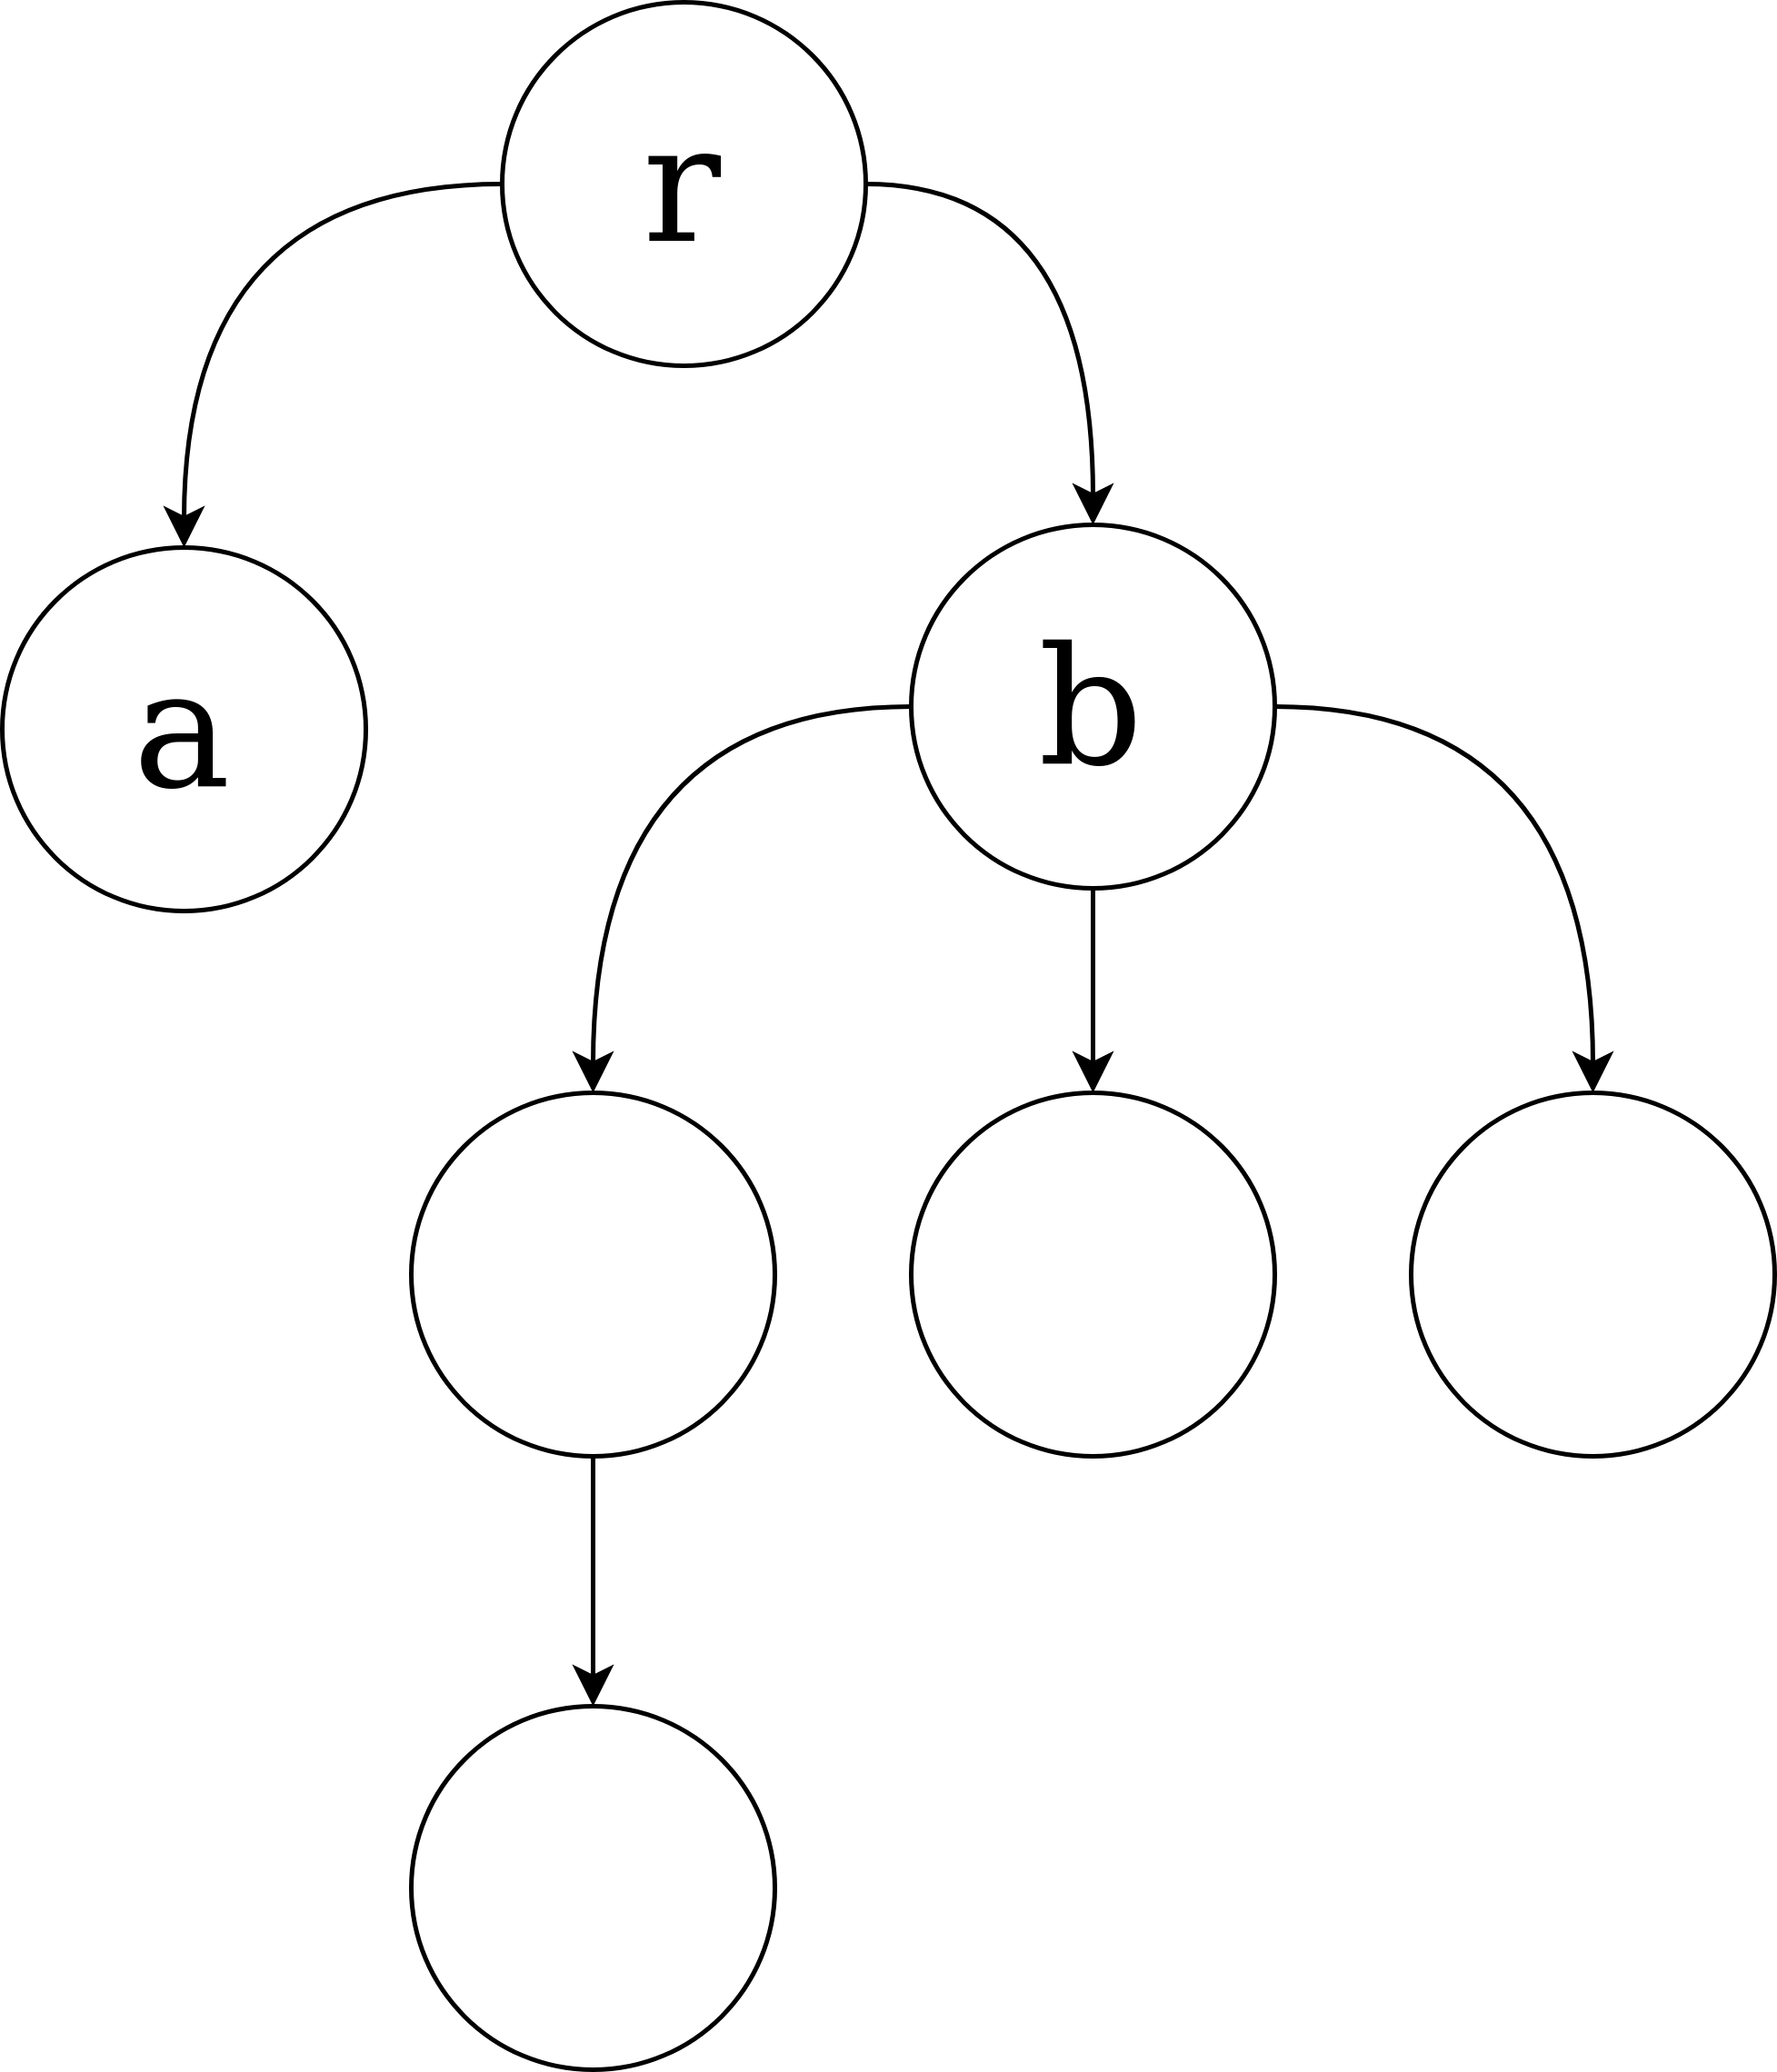
\includegraphics[width=0.5\linewidth]{HDS.png}
\end{figure}

Figure~\ref{non-HDS} contains example of data structures, that are not hierarchical. Figure~\ref{non-HDS-1-pic} presents a data structure, that has two nodes without a parent (nodes \texttt{a} and \texttt{b}), while a hierarchical data structure can contain only one such node. Figure~\ref{non-HDS-2-pic} presents a data structure with a loop, consisting of nodes \texttt{a}, \texttt{b}, and \texttt{c}. Figure~\ref{non-HDS-3-pic} presents data structure, in which node \texttt{c} has two parents simultaneously: nodes \texttt{a} and \texttt{b}.

\begin{figure}[H]
     \centering
     \begin{subfigure}[b]{0.35\linewidth}
          \centering
          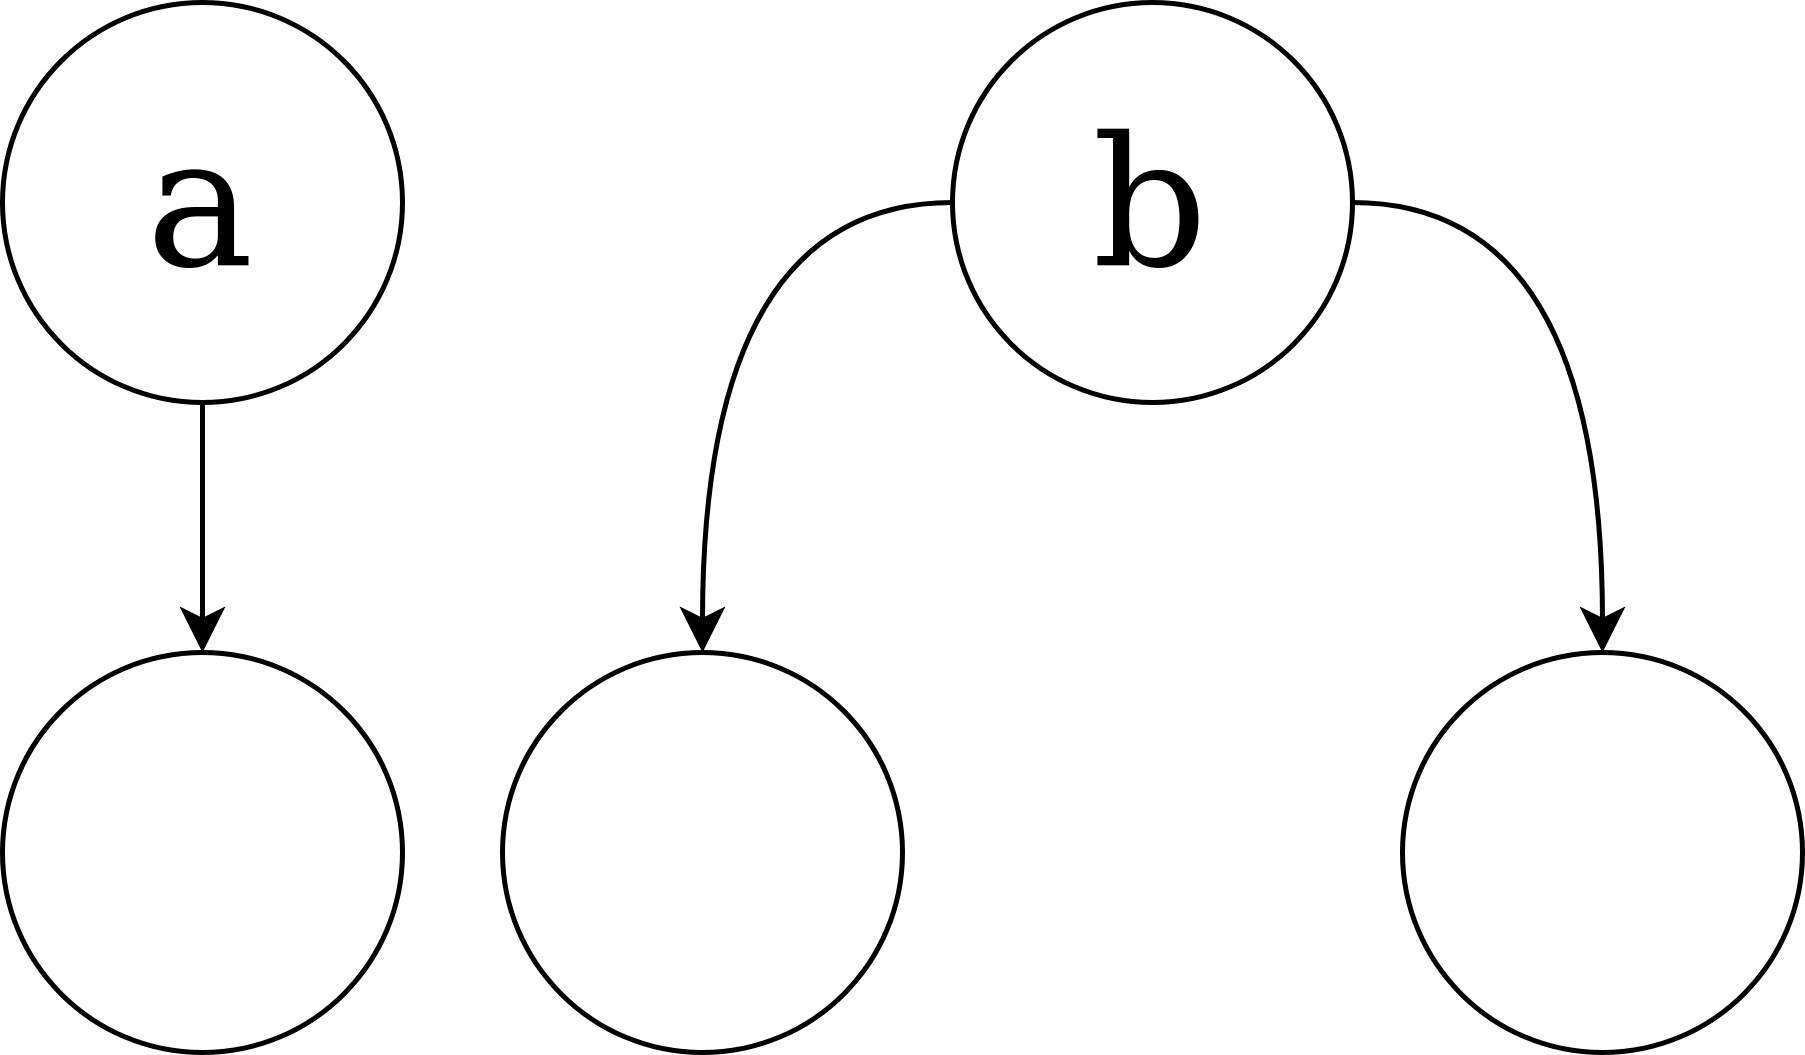
\includegraphics[width=\linewidth]{non-HDS-1.png}
          \captionof{figure}{Data structure with two root nodes}
          \label{non-HDS-1-pic}
     \end{subfigure}
     \hfill
     \begin{subfigure}[b]{0.25\linewidth}
          \centering
          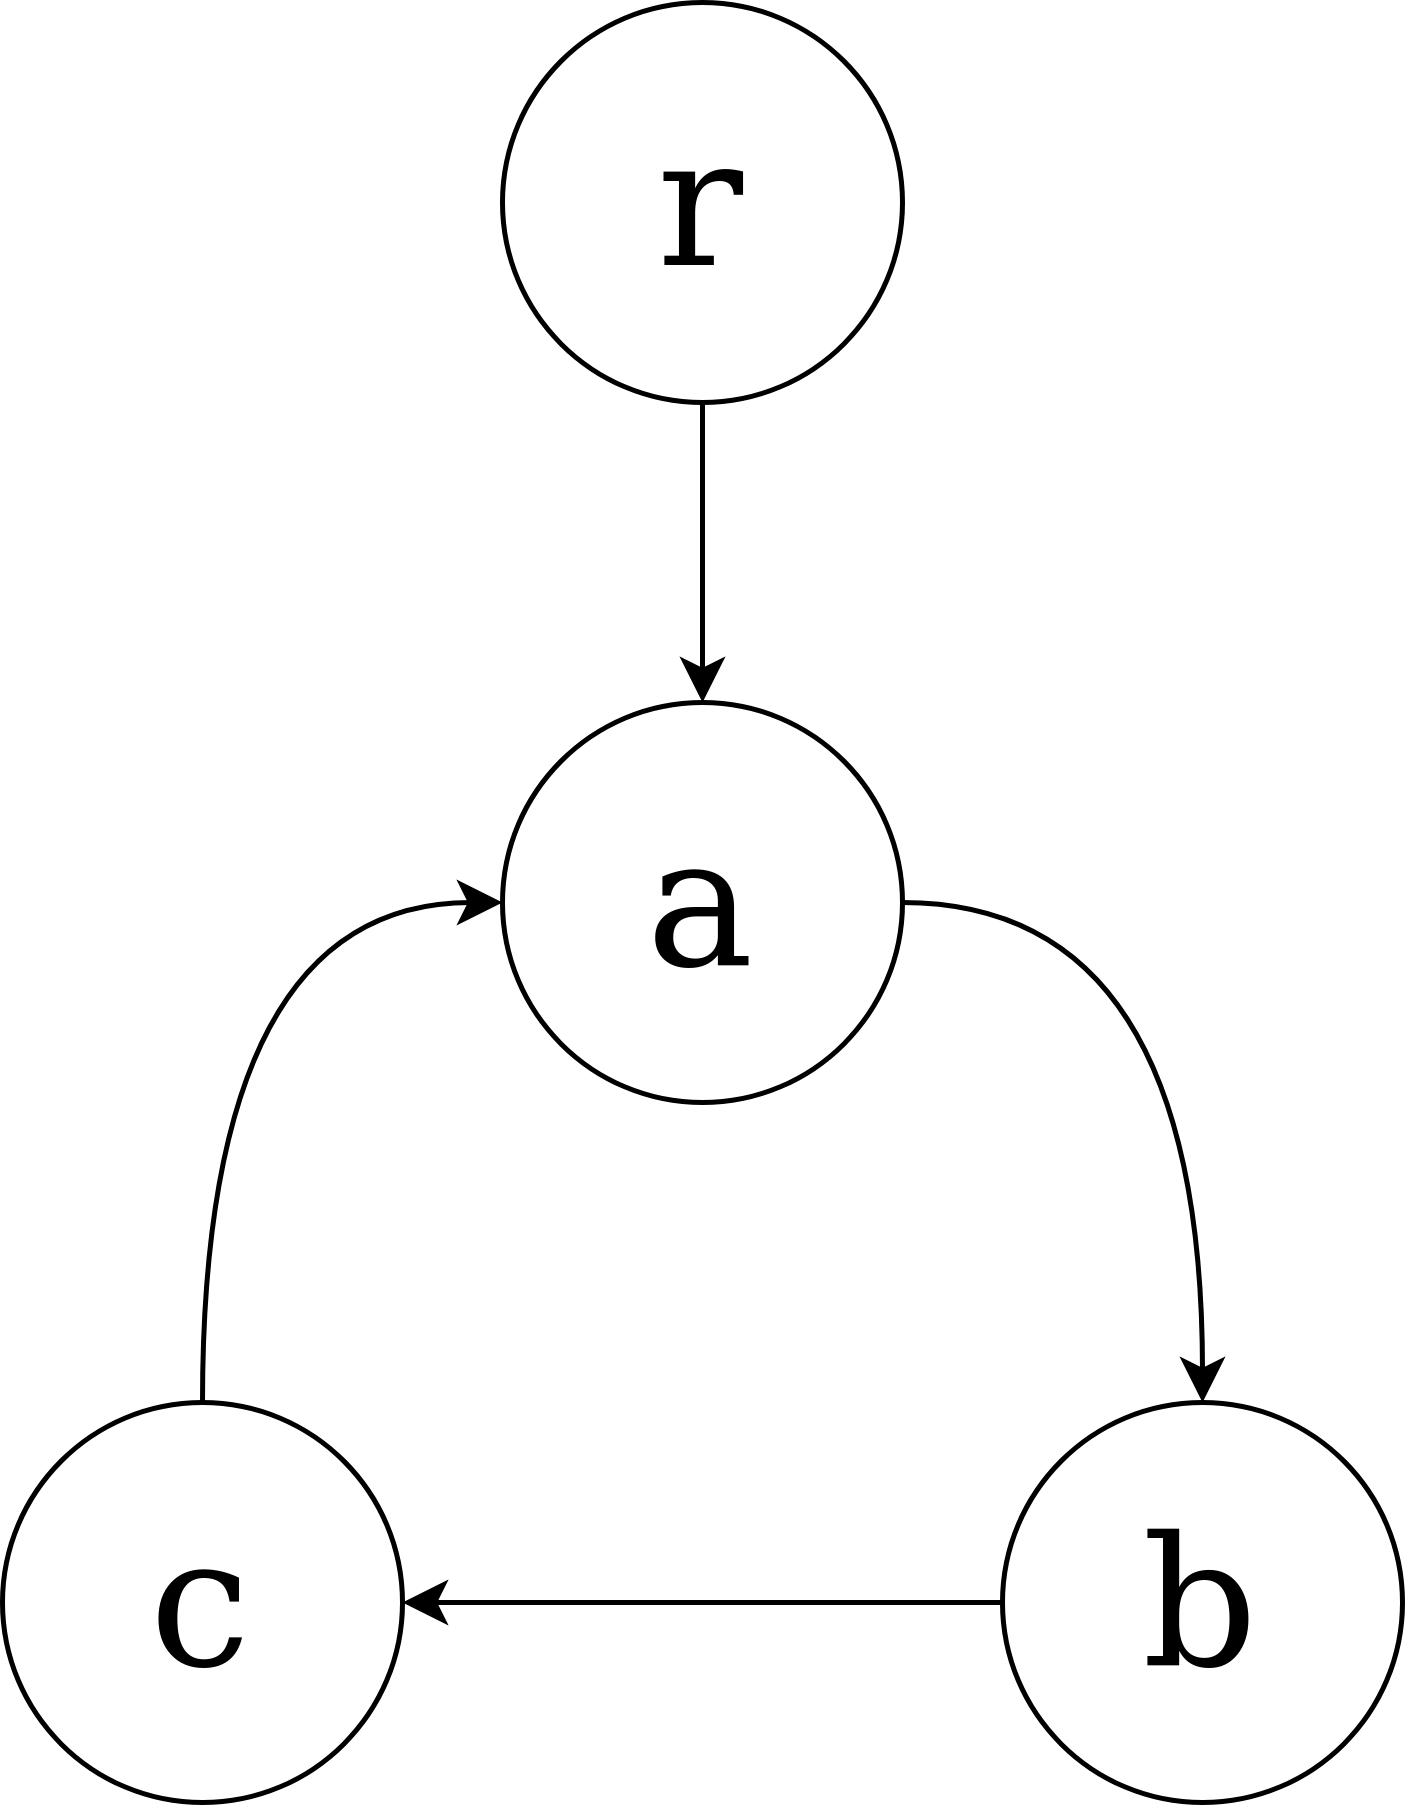
\includegraphics[width=\linewidth]{non-HDS-2.png}
          \captionof{figure}{Data structure with a loop}
          \label{non-HDS-2-pic}
     \end{subfigure}
     \hfill
     \begin{subfigure}[b]{0.25\linewidth}
          \centering
          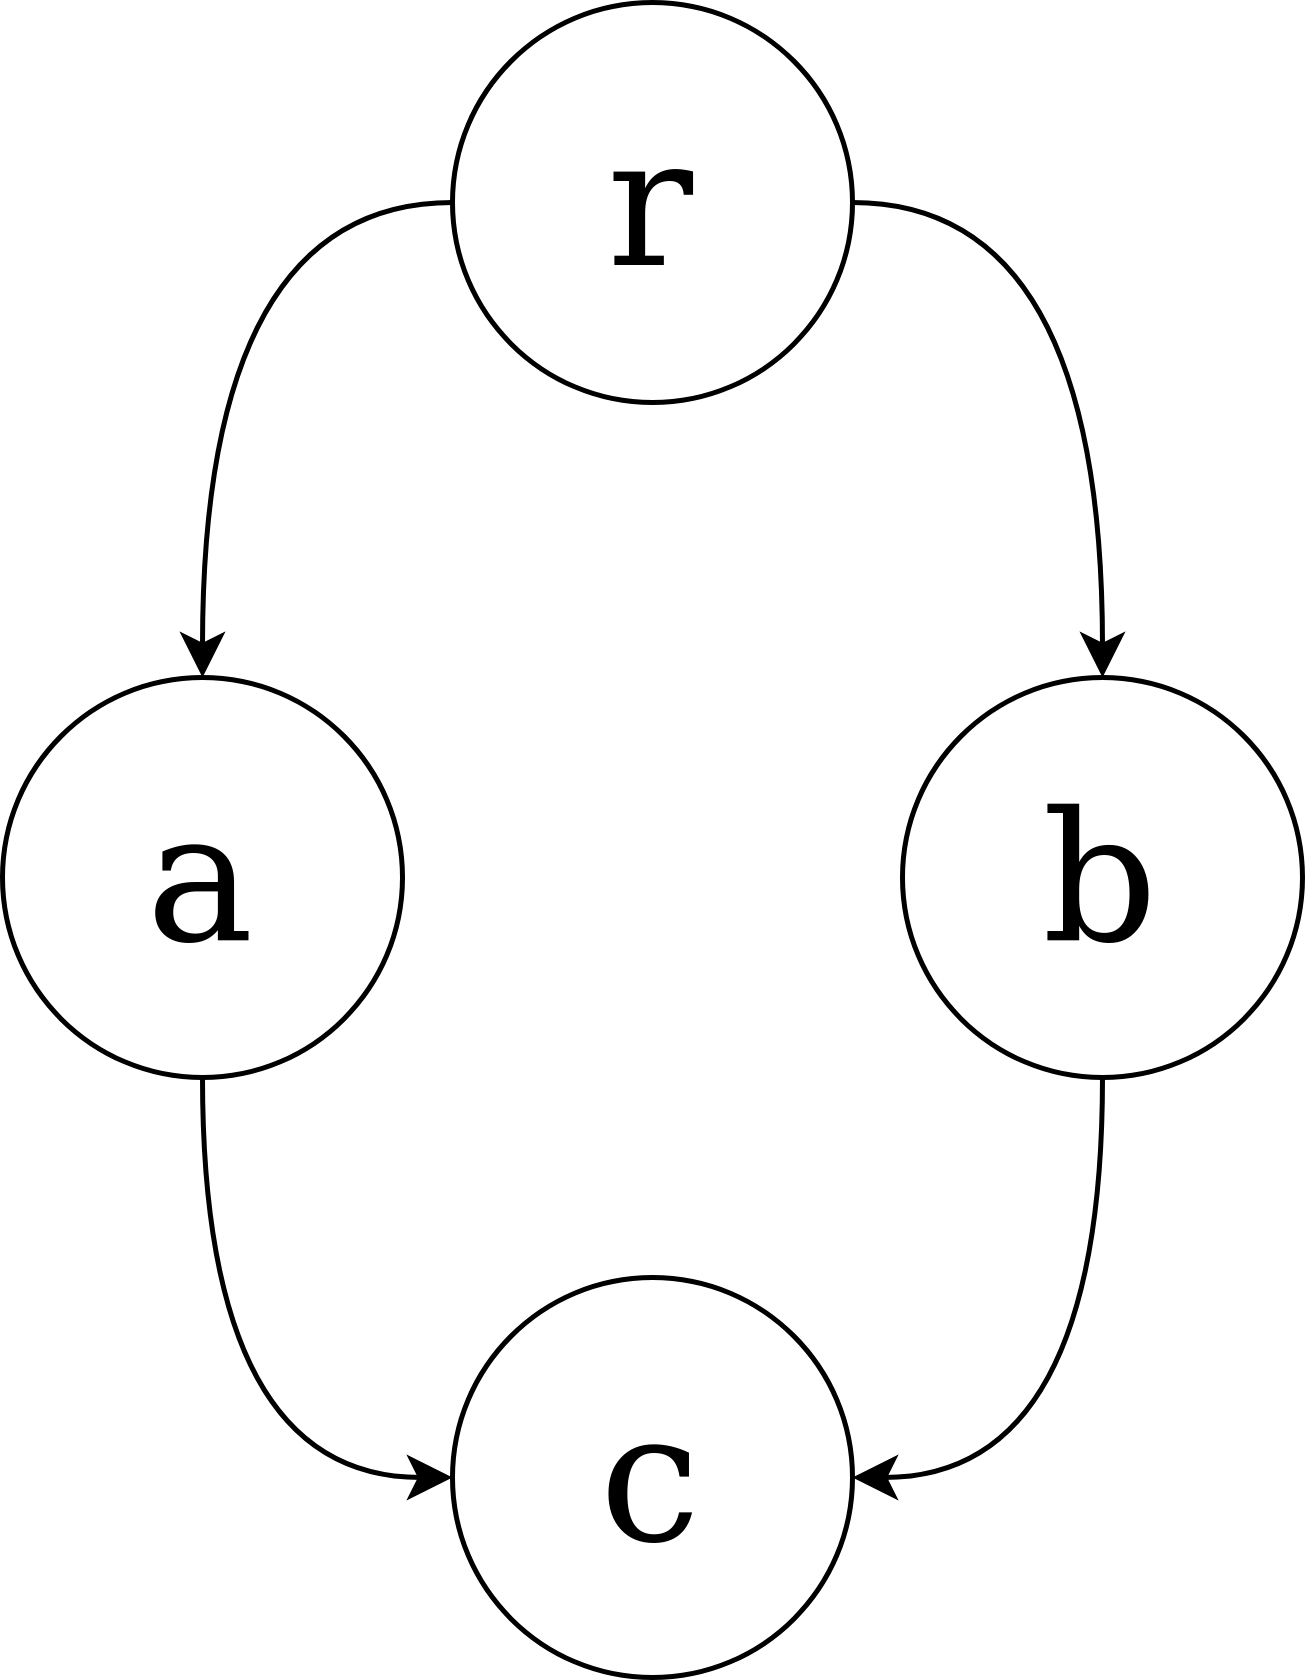
\includegraphics[width=\linewidth]{non-HDS-3.png}
          \captionof{figure}{Data structure, in which a node has two parents}
          \label{non-HDS-3-pic}
     \end{subfigure}
    \caption{Examples of data structures, that are not trees}
    \label{non-HDS}
\end{figure}

Trees are defined in~\cite{tree-definition}.

Multiple kind of trees have been studied in the literature. Amongst the most useful ones we may outline binary search trees~\cite{cormen2022introduction} (Fig.~\ref{bin-search-tree-pic}), quad trees~\cite{de2000computational} (Fig.~\ref{quad-tree-pic}) and tries~\cite{bodon2003trie} (Fig~\ref{trie-pic}). Algorithm, that we will design and implement in that work, will work with all of them, and with various other kind of trees.

\begin{figure}[H]
  \centering
  \caption{Example of a binary search tree}
  \label{bin-search-tree-pic}
  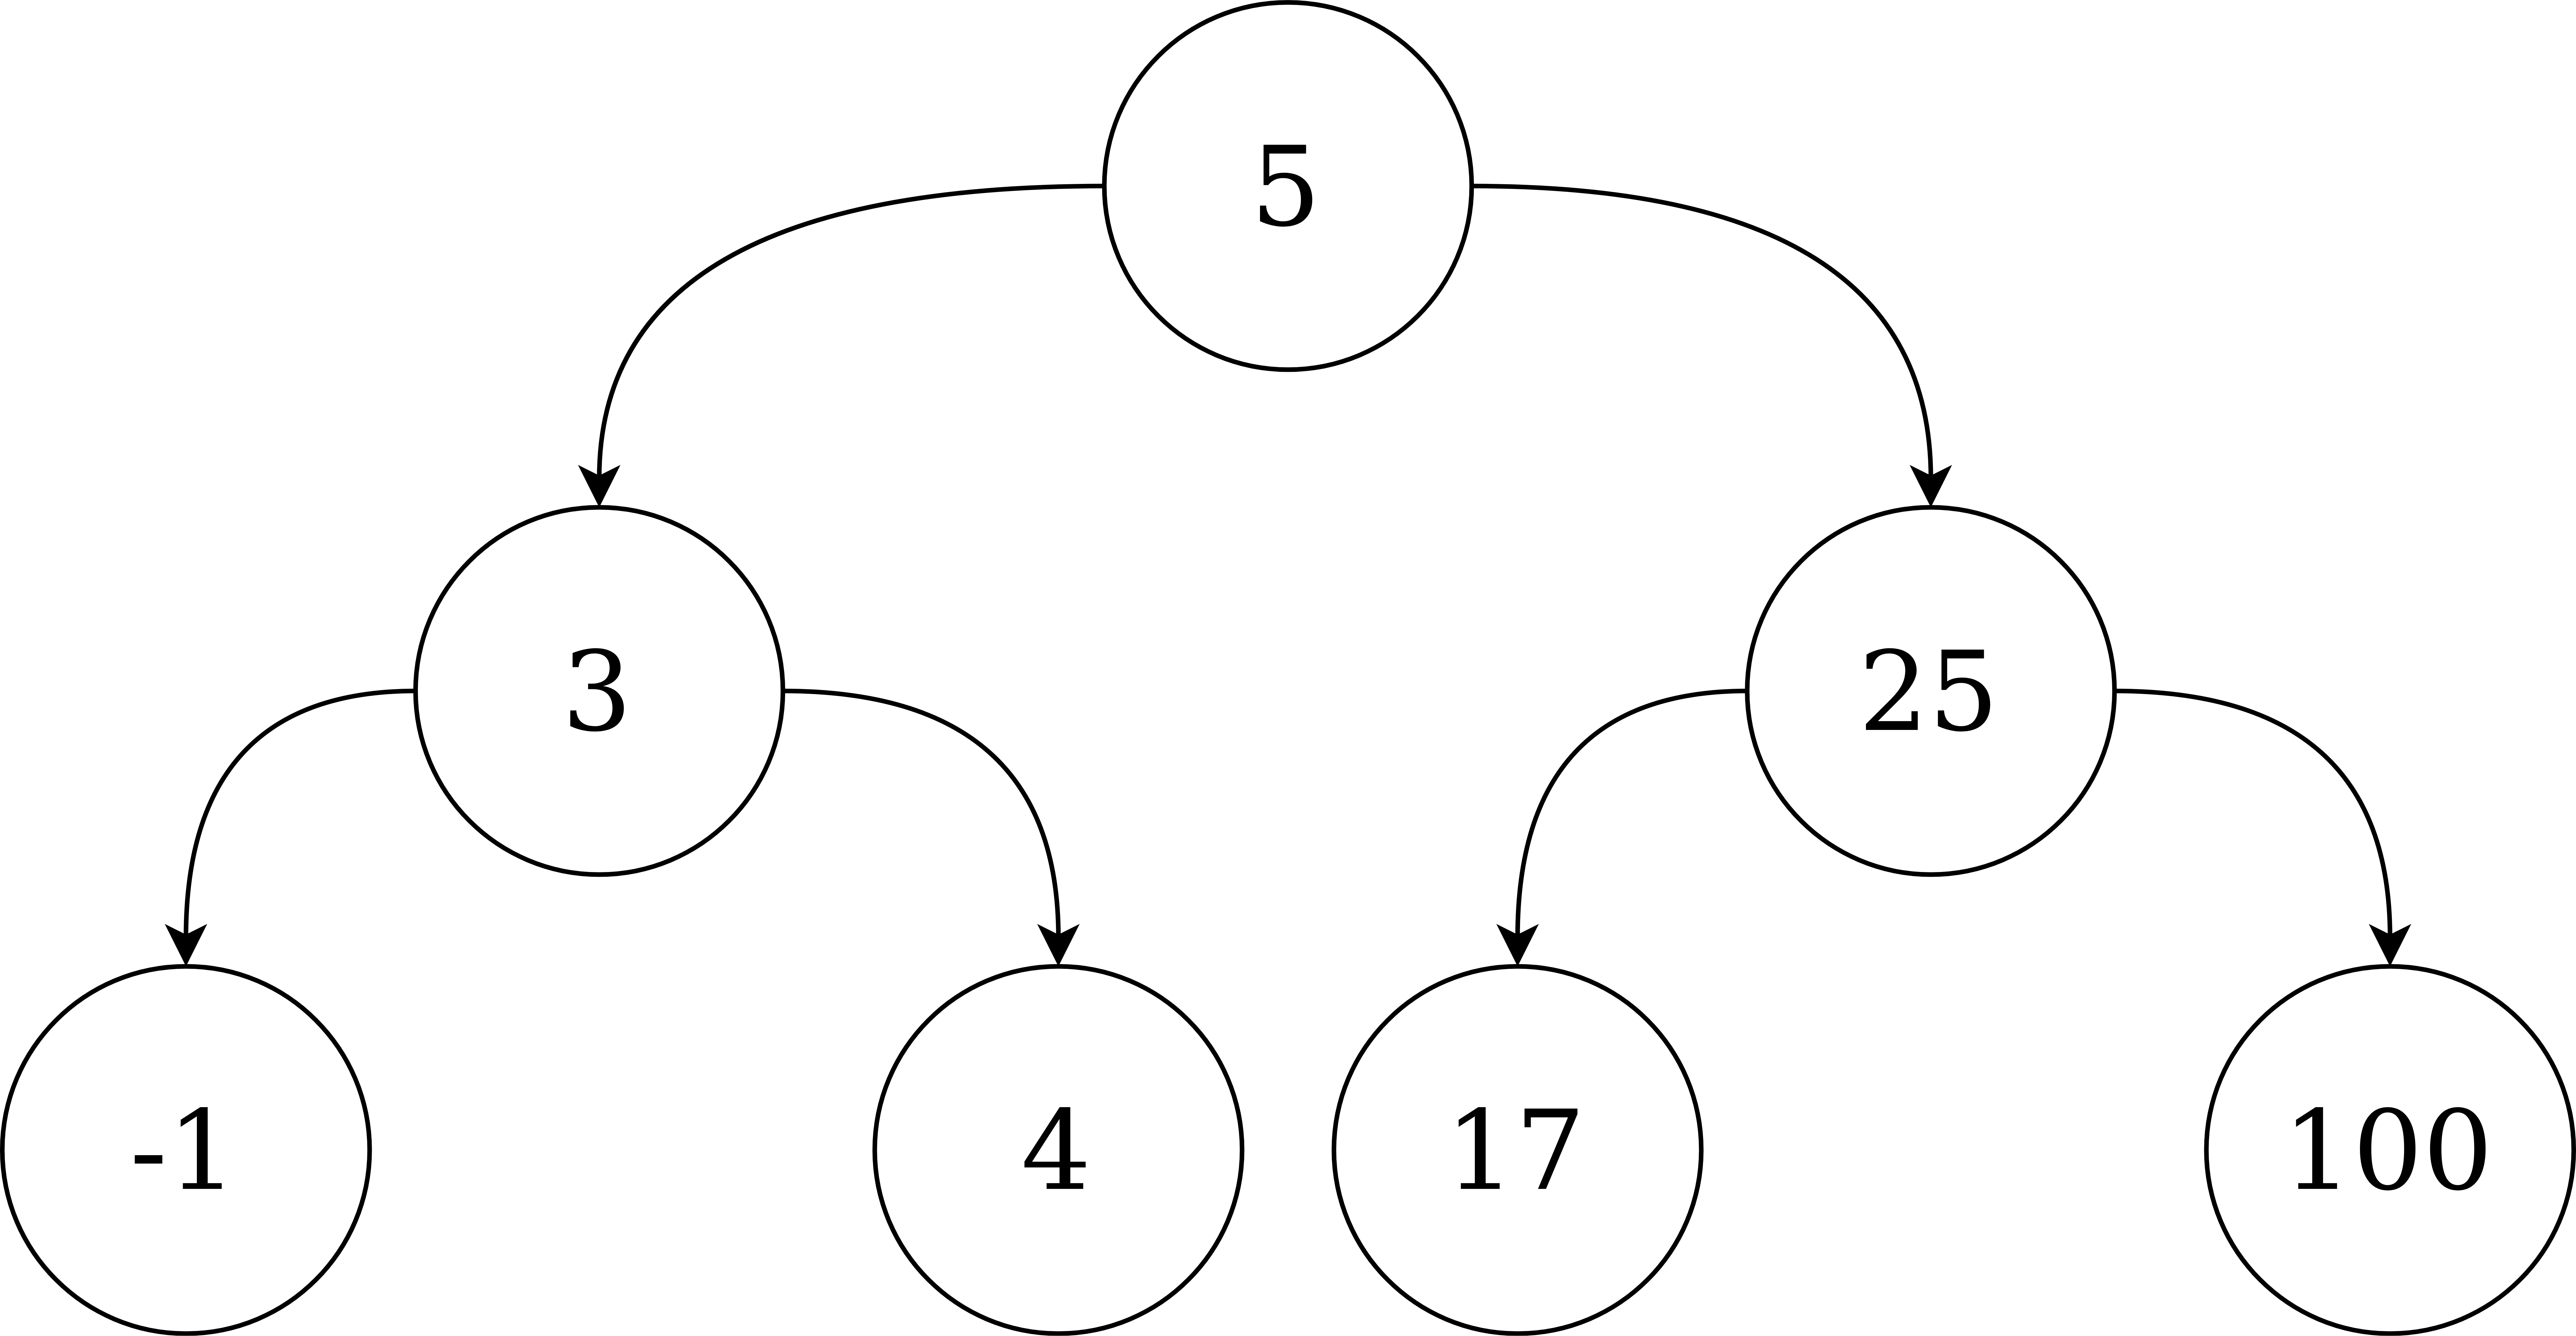
\includegraphics[width=\linewidth]{pics/bin-search-tree.png}
\end{figure}

\begin{figure}[H]
  \centering
  \caption{Example of a quad tree}
  \label{quad-tree-pic}
  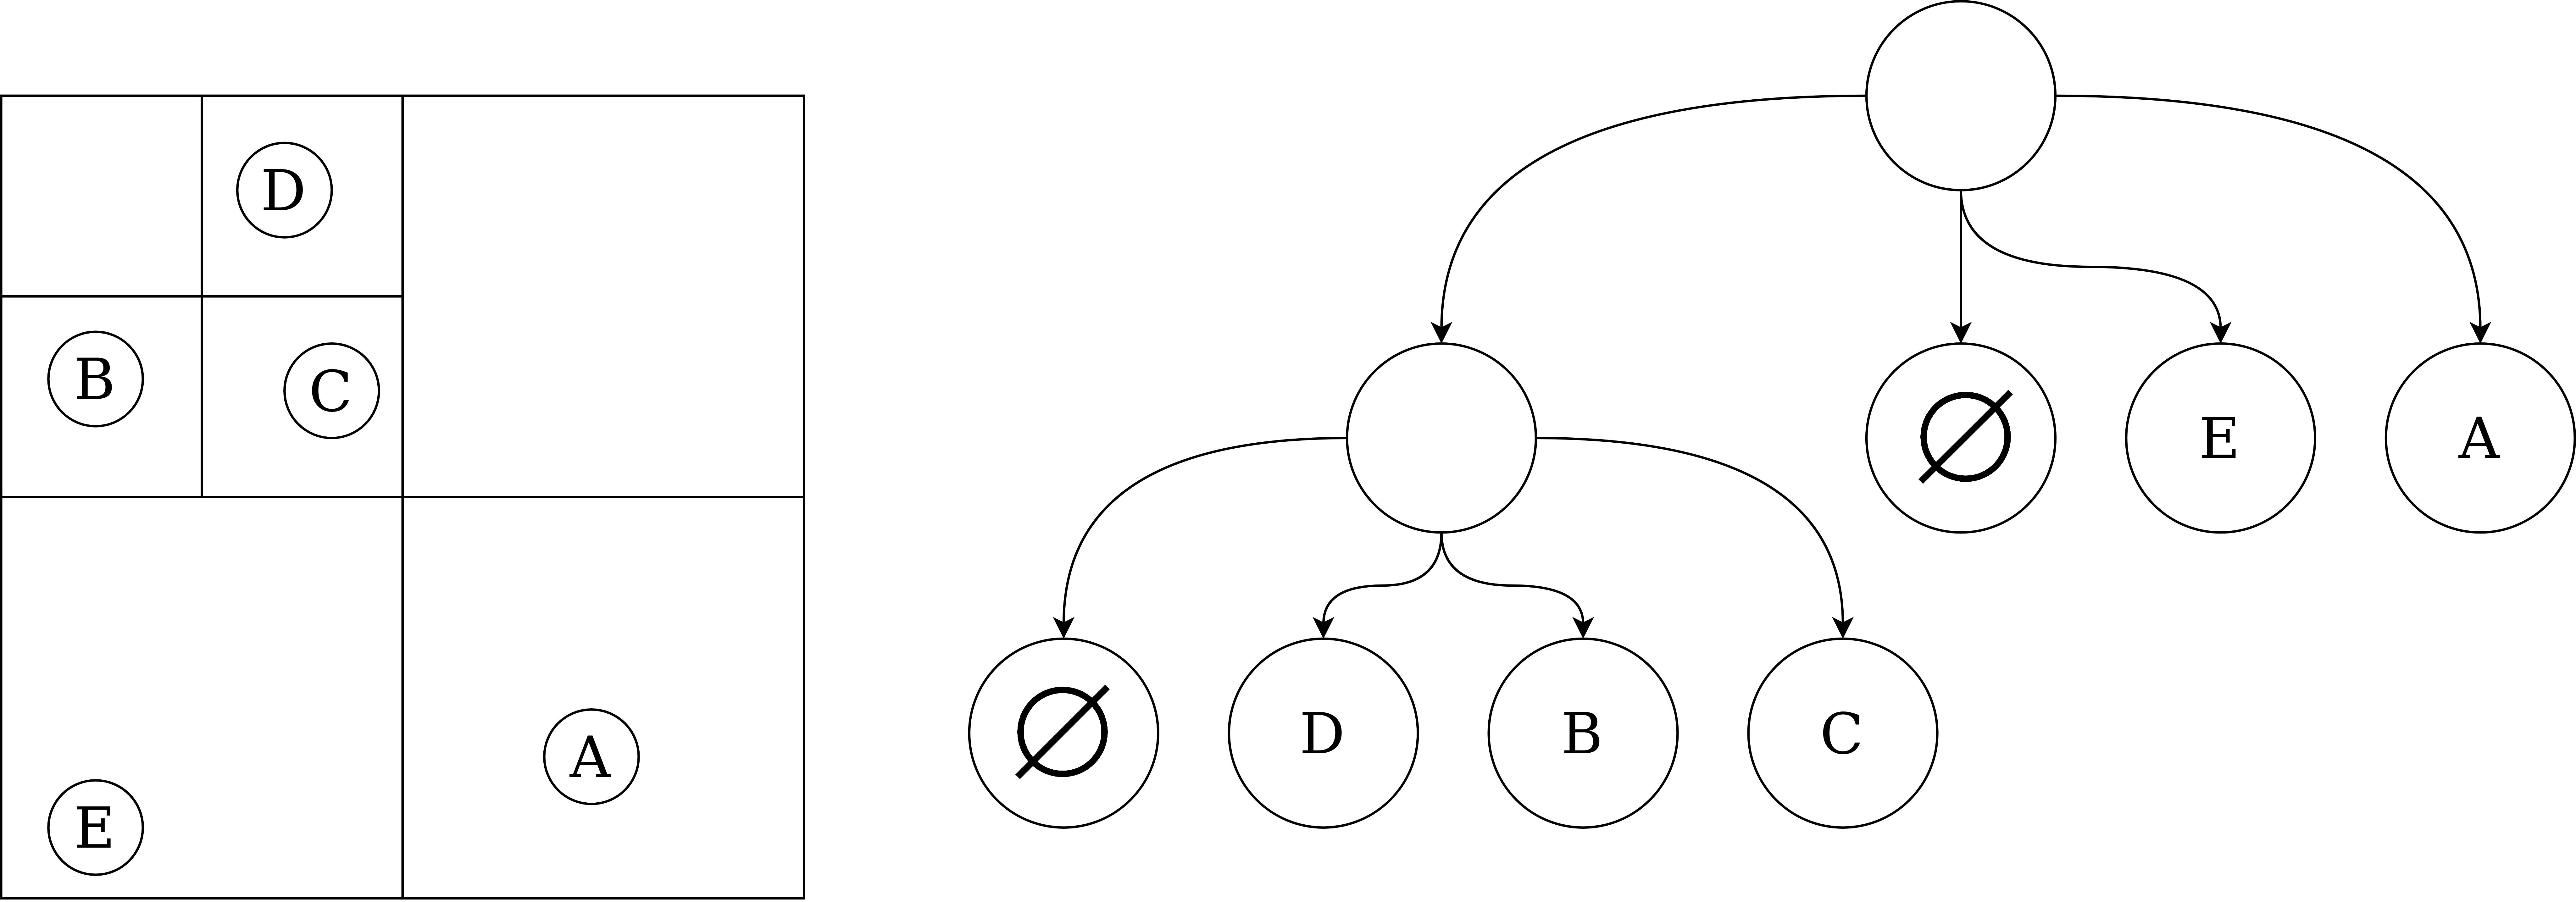
\includegraphics[width=\linewidth]{pics/quad-tree.png}
\end{figure}

\begin{figure}[H]
  \centering
  \caption{Example of a trie}
  \label{trie-pic}
  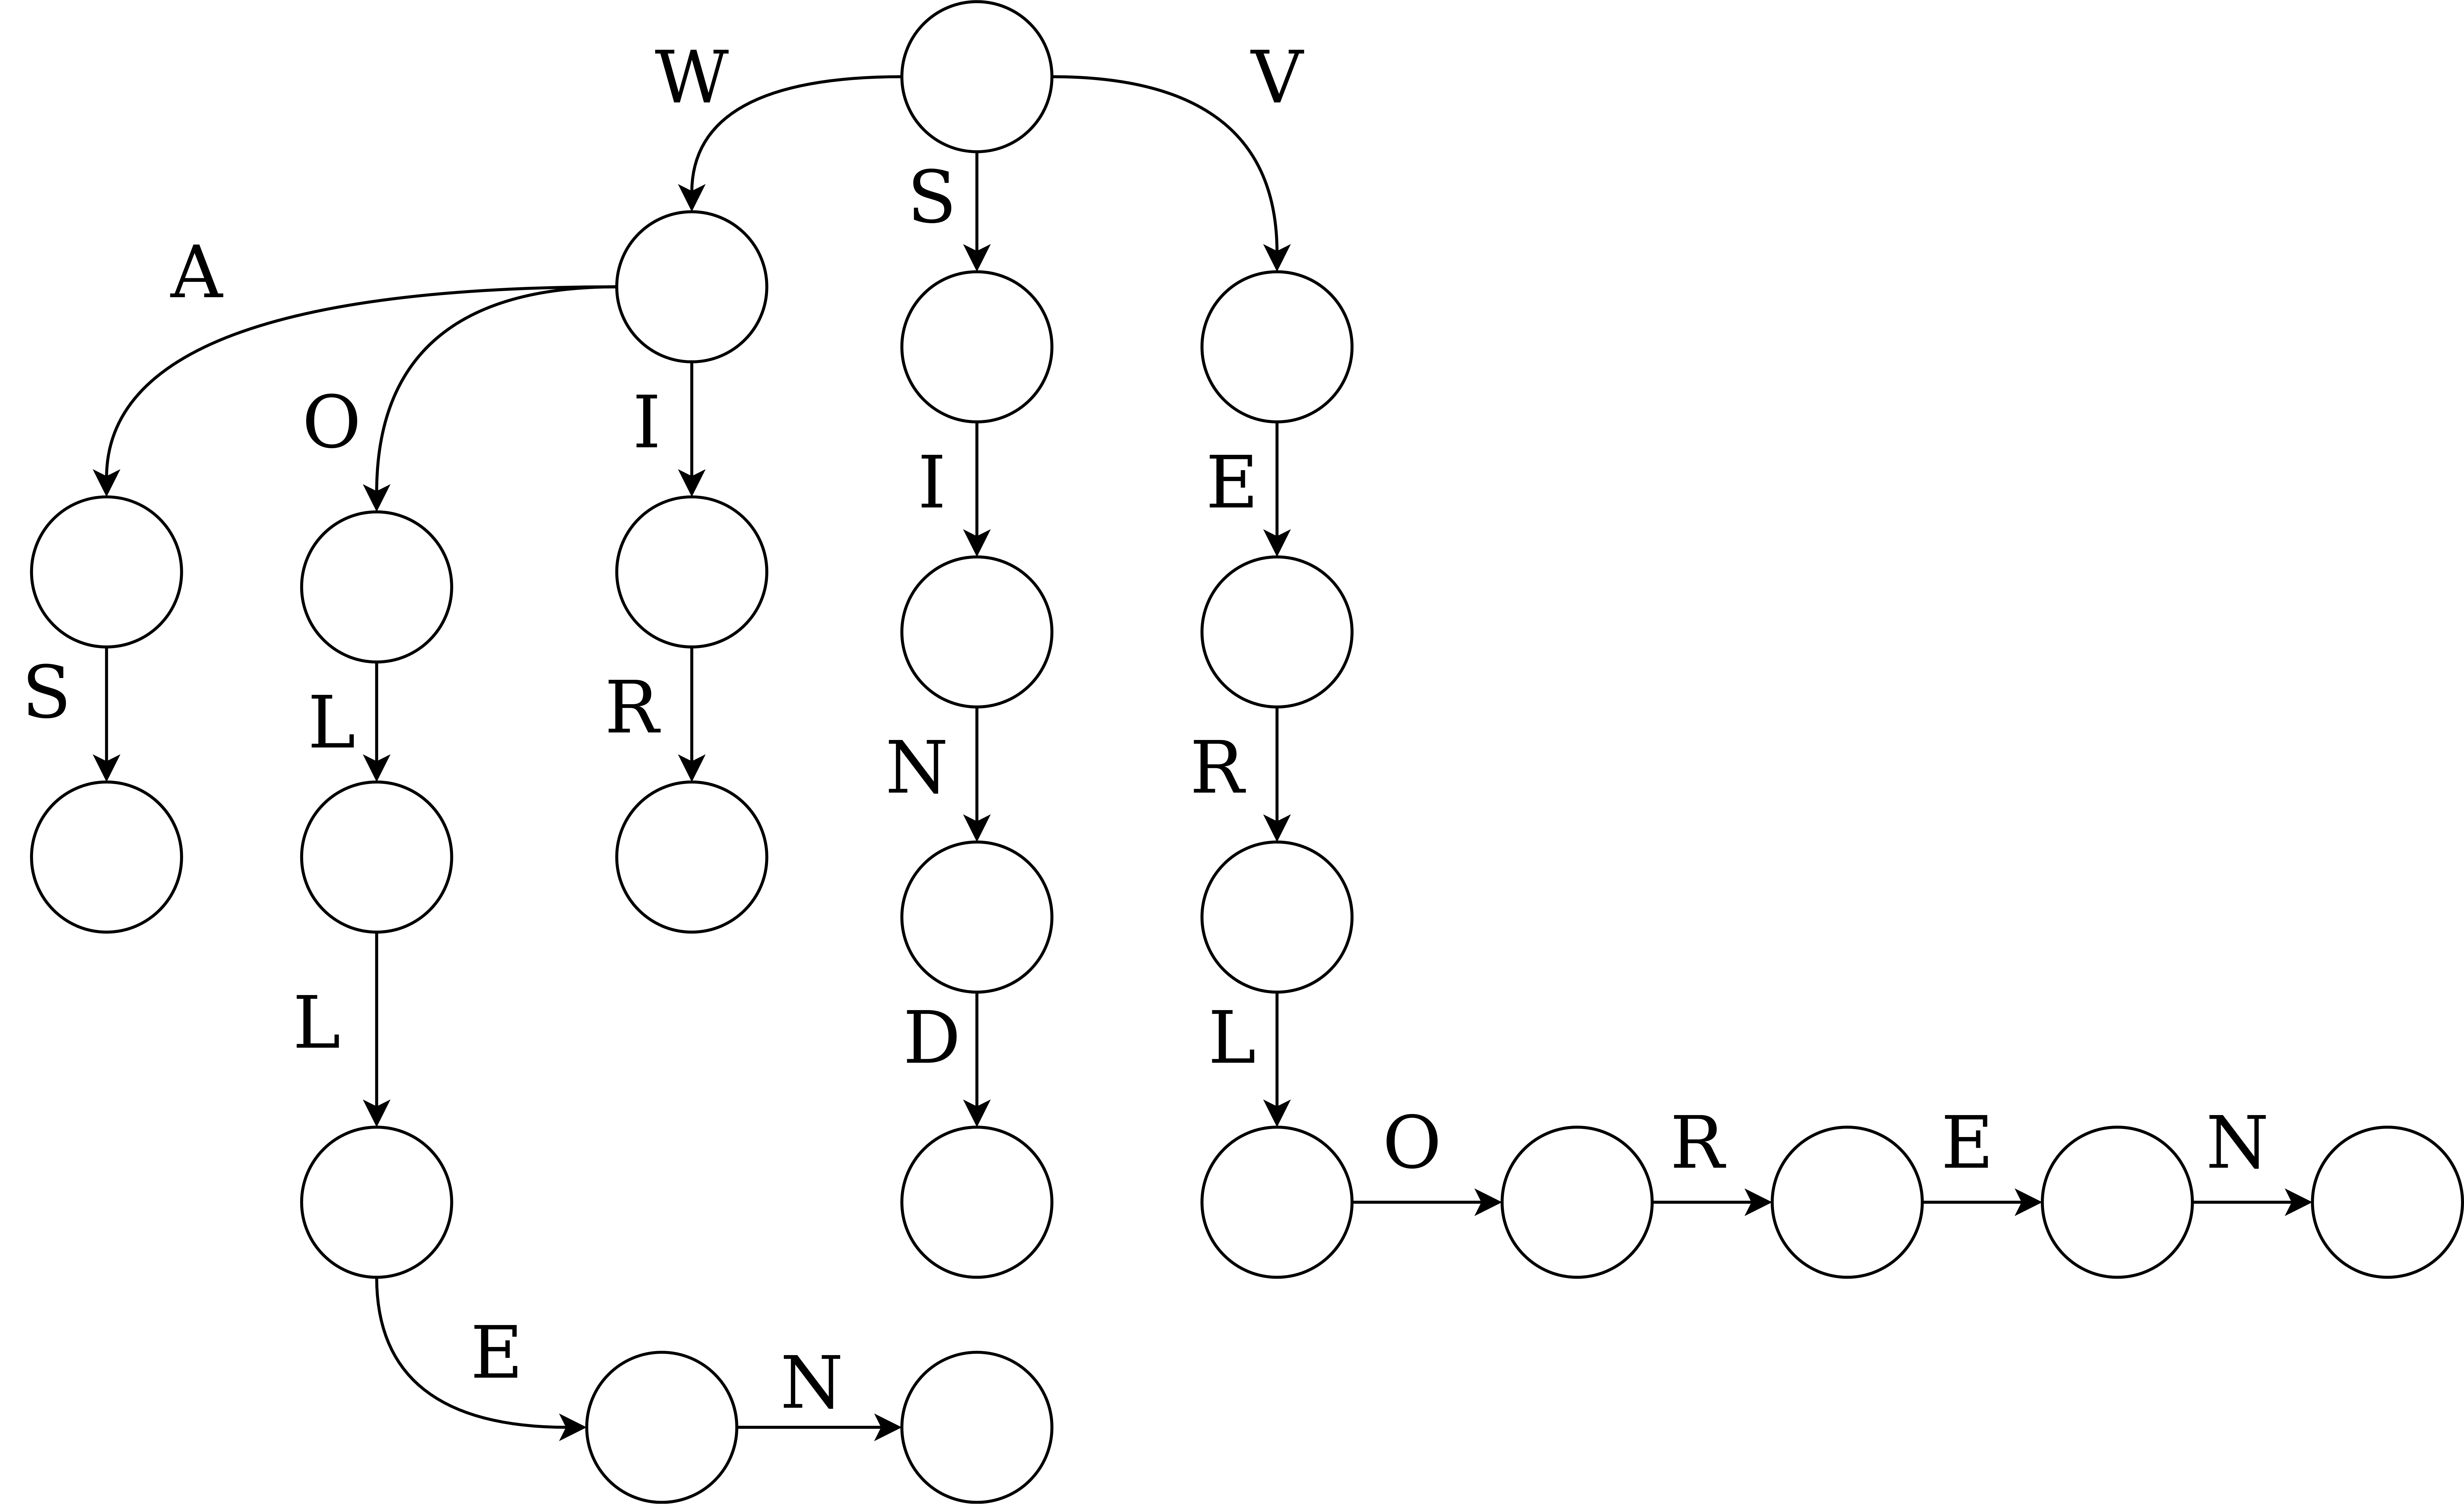
\includegraphics[width=\linewidth]{pics/trie.png}
\end{figure}


\section{Range queries}

\begin{definition}
Consider a tree, storing multiple data items. We call a query, retrieving or modifying a single data item, a \emph{scalar query}; and a query, involving multiple consecutive (by value) data items, a \emph{range query}. 
\end{definition}
\bigbreak

Consider a sorted set, stored in a binary search tree. In this case, the following queries are scalar:

\begin{itemize}
    \item \texttt{insert(key)}~--- if \texttt{key} exists in the data set, do not modify the set and return \texttt{false}. Otherwise, add \texttt{key} to the set and return \texttt{true}.
    
    \item \texttt{remove(key)}~--- if \texttt{key} does not exist in the set, do not modify the set and return \texttt{false}. Otherwise, remove \texttt{key} from the set and return \texttt{true}.
    
    \item \texttt{contains(key)}~--- return \texttt{true} if the set contains \texttt{key}, \texttt{false}, otherwise.
\end{itemize} 

\bigbreak
And the following queries are range queries:

\begin{itemize}
    \item \texttt{count(min, max)}~--- returns the number of keys from the \texttt{[min; max]} interval.
    
    \item \texttt{collect(min, max)}~--- returns an array of set keys from the \texttt{[min; max]} interval.
\end{itemize}

\section{Efficient sequential algorithm for range queries}
\label{sequential-algorithm}

Many range queries, especially the aggregating ones, can be executed in sub-linear (e.g. logarithmic) time. Consider, an example of such range query: \newline \texttt{count(Set, min, max) = $\mid \{$ x $\in$ Set : min $\leq$ x $\leq$ max $\} \mid$}~--- the number of keys, located in the range \texttt{[min; max]}. It can be calculated in $O(\log N)$ time on binary search trees (where $N$ is the number of keys in the set), using the following algorithm.

\subsection{Tree structure}

Let us begin with a couple of definitions:

\bigbreak

\begin{definition}
A node is a \emph{leaf} if it has no children.
\end{definition}

\begin{definition}
A node is an \emph{internal} node if it is not a leaf.
\end{definition}

\begin{definition}
\emph{External} binary search tree (Fig.~\ref{external-tree-pic}) is a binary search tree, in which keys are stored only in leaf nodes. In contrast, internal nodes store only auxiliary information, used for query routing (e.g., the minimal key, that might be located in the right subtree).
\end{definition}

\begin{definition}
\emph{Internal} binary search tree (Fig.~\ref{internal-tree-pic}) is a binary search tree, in which keys are stored in both leaf nodes and in internal nodes.
\end{definition}

\begin{figure}[H]
     \centering
     \begin{subfigure}[b]{0.55\linewidth}
          \centering
          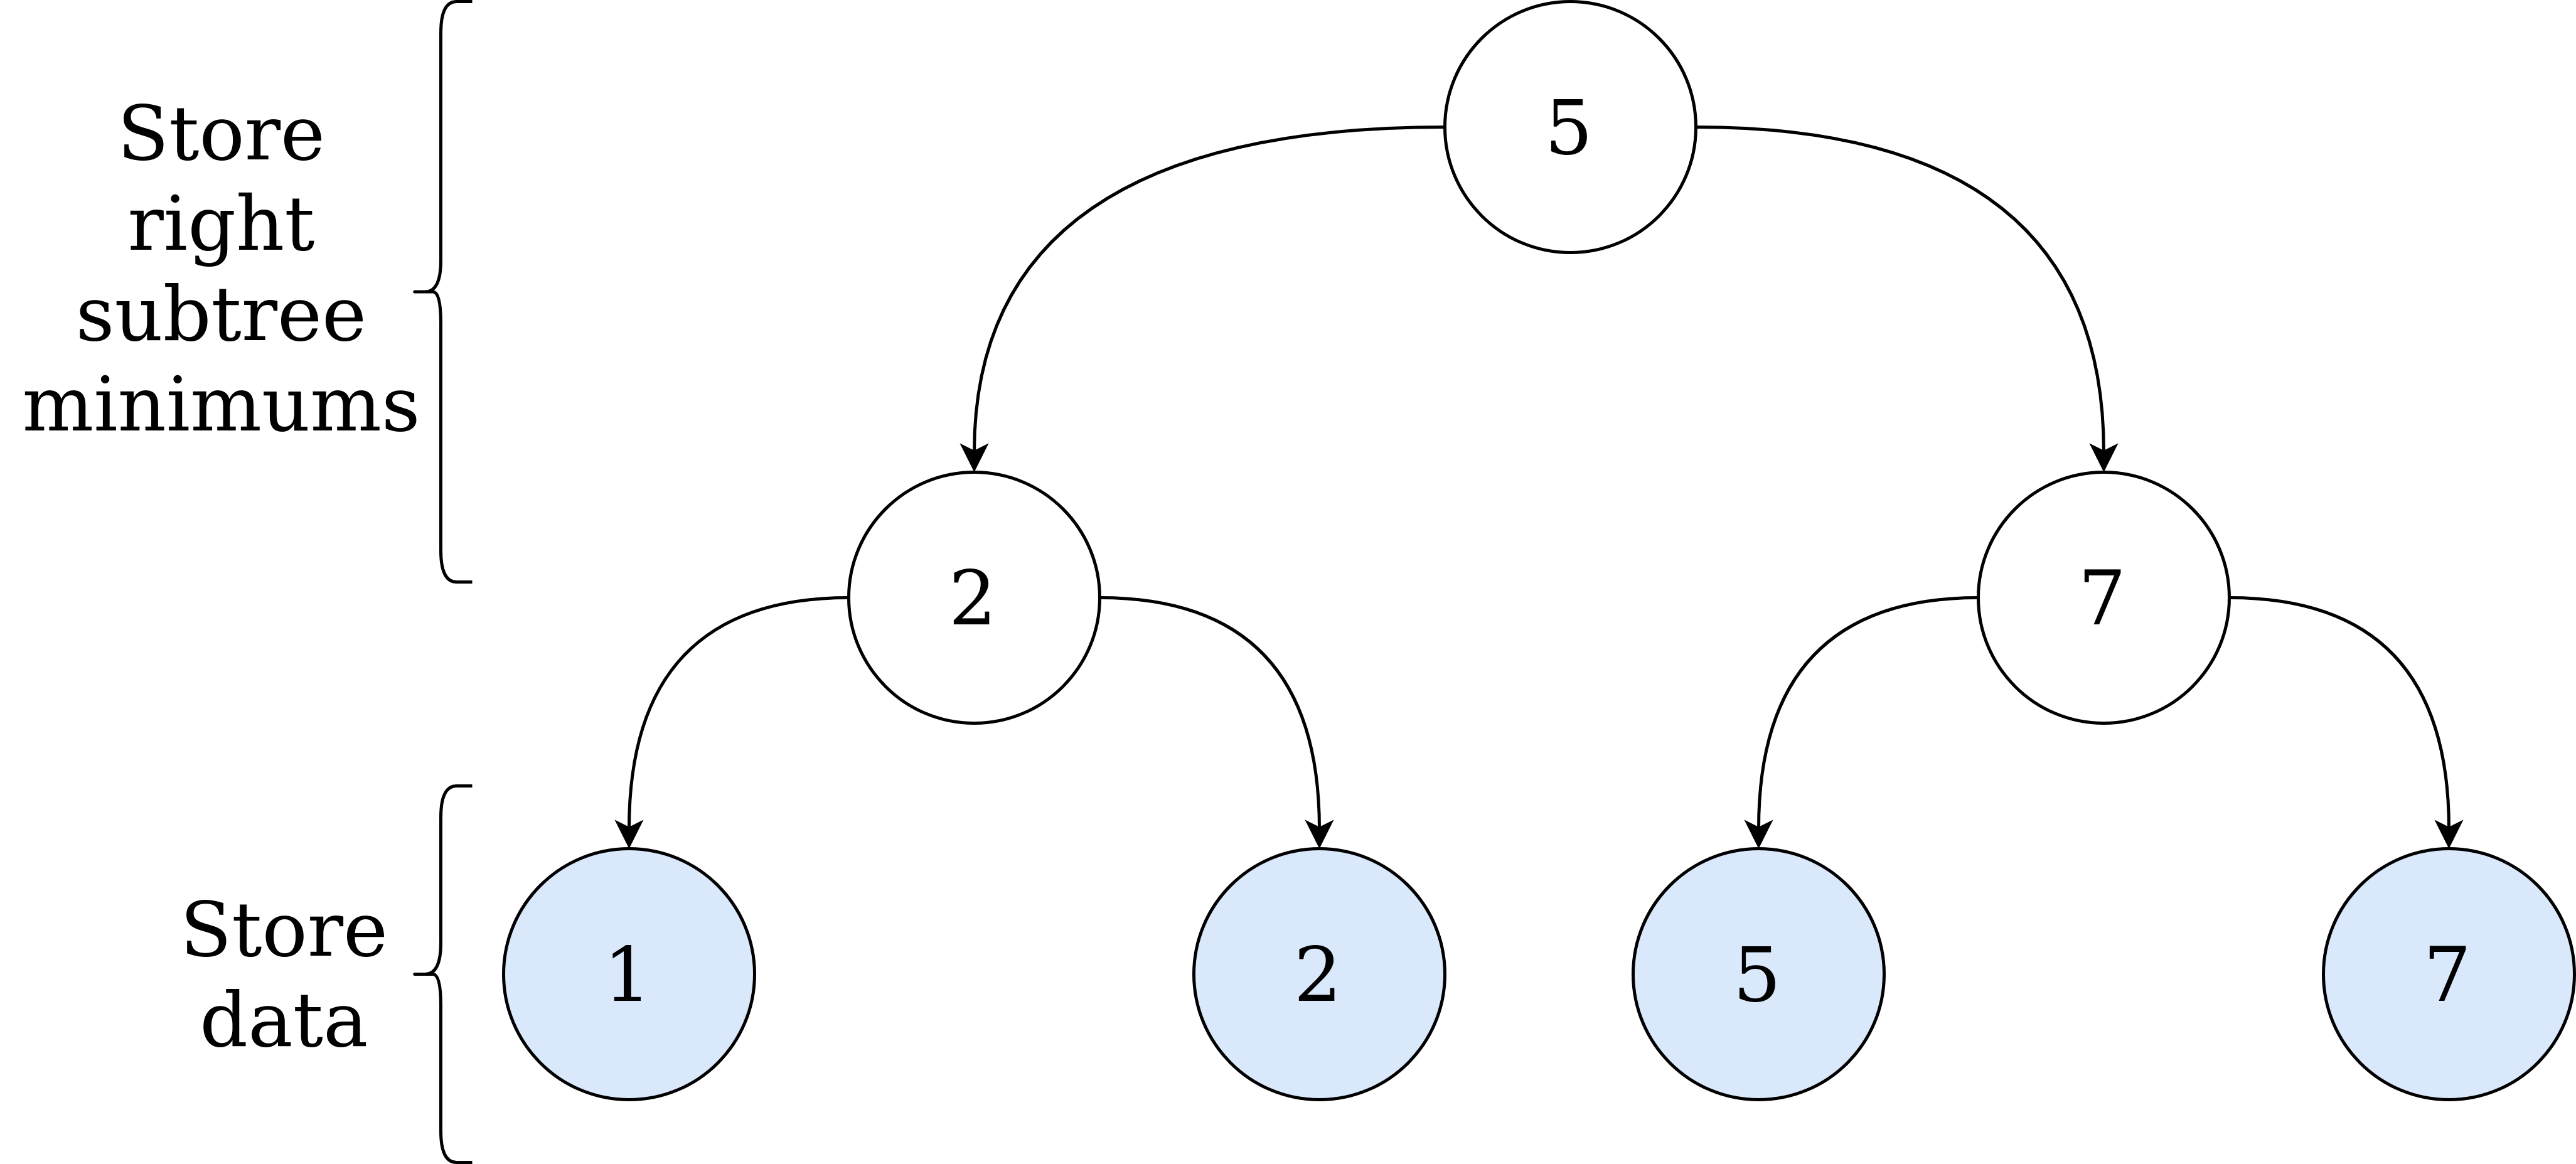
\includegraphics[width=\linewidth]{pics/external-tree.png}
          \captionof{figure}{External binary search tree}
          \label{external-tree-pic}
     \end{subfigure}
     \hfill
     \begin{subfigure}[b]{0.35\linewidth}
          \centering
          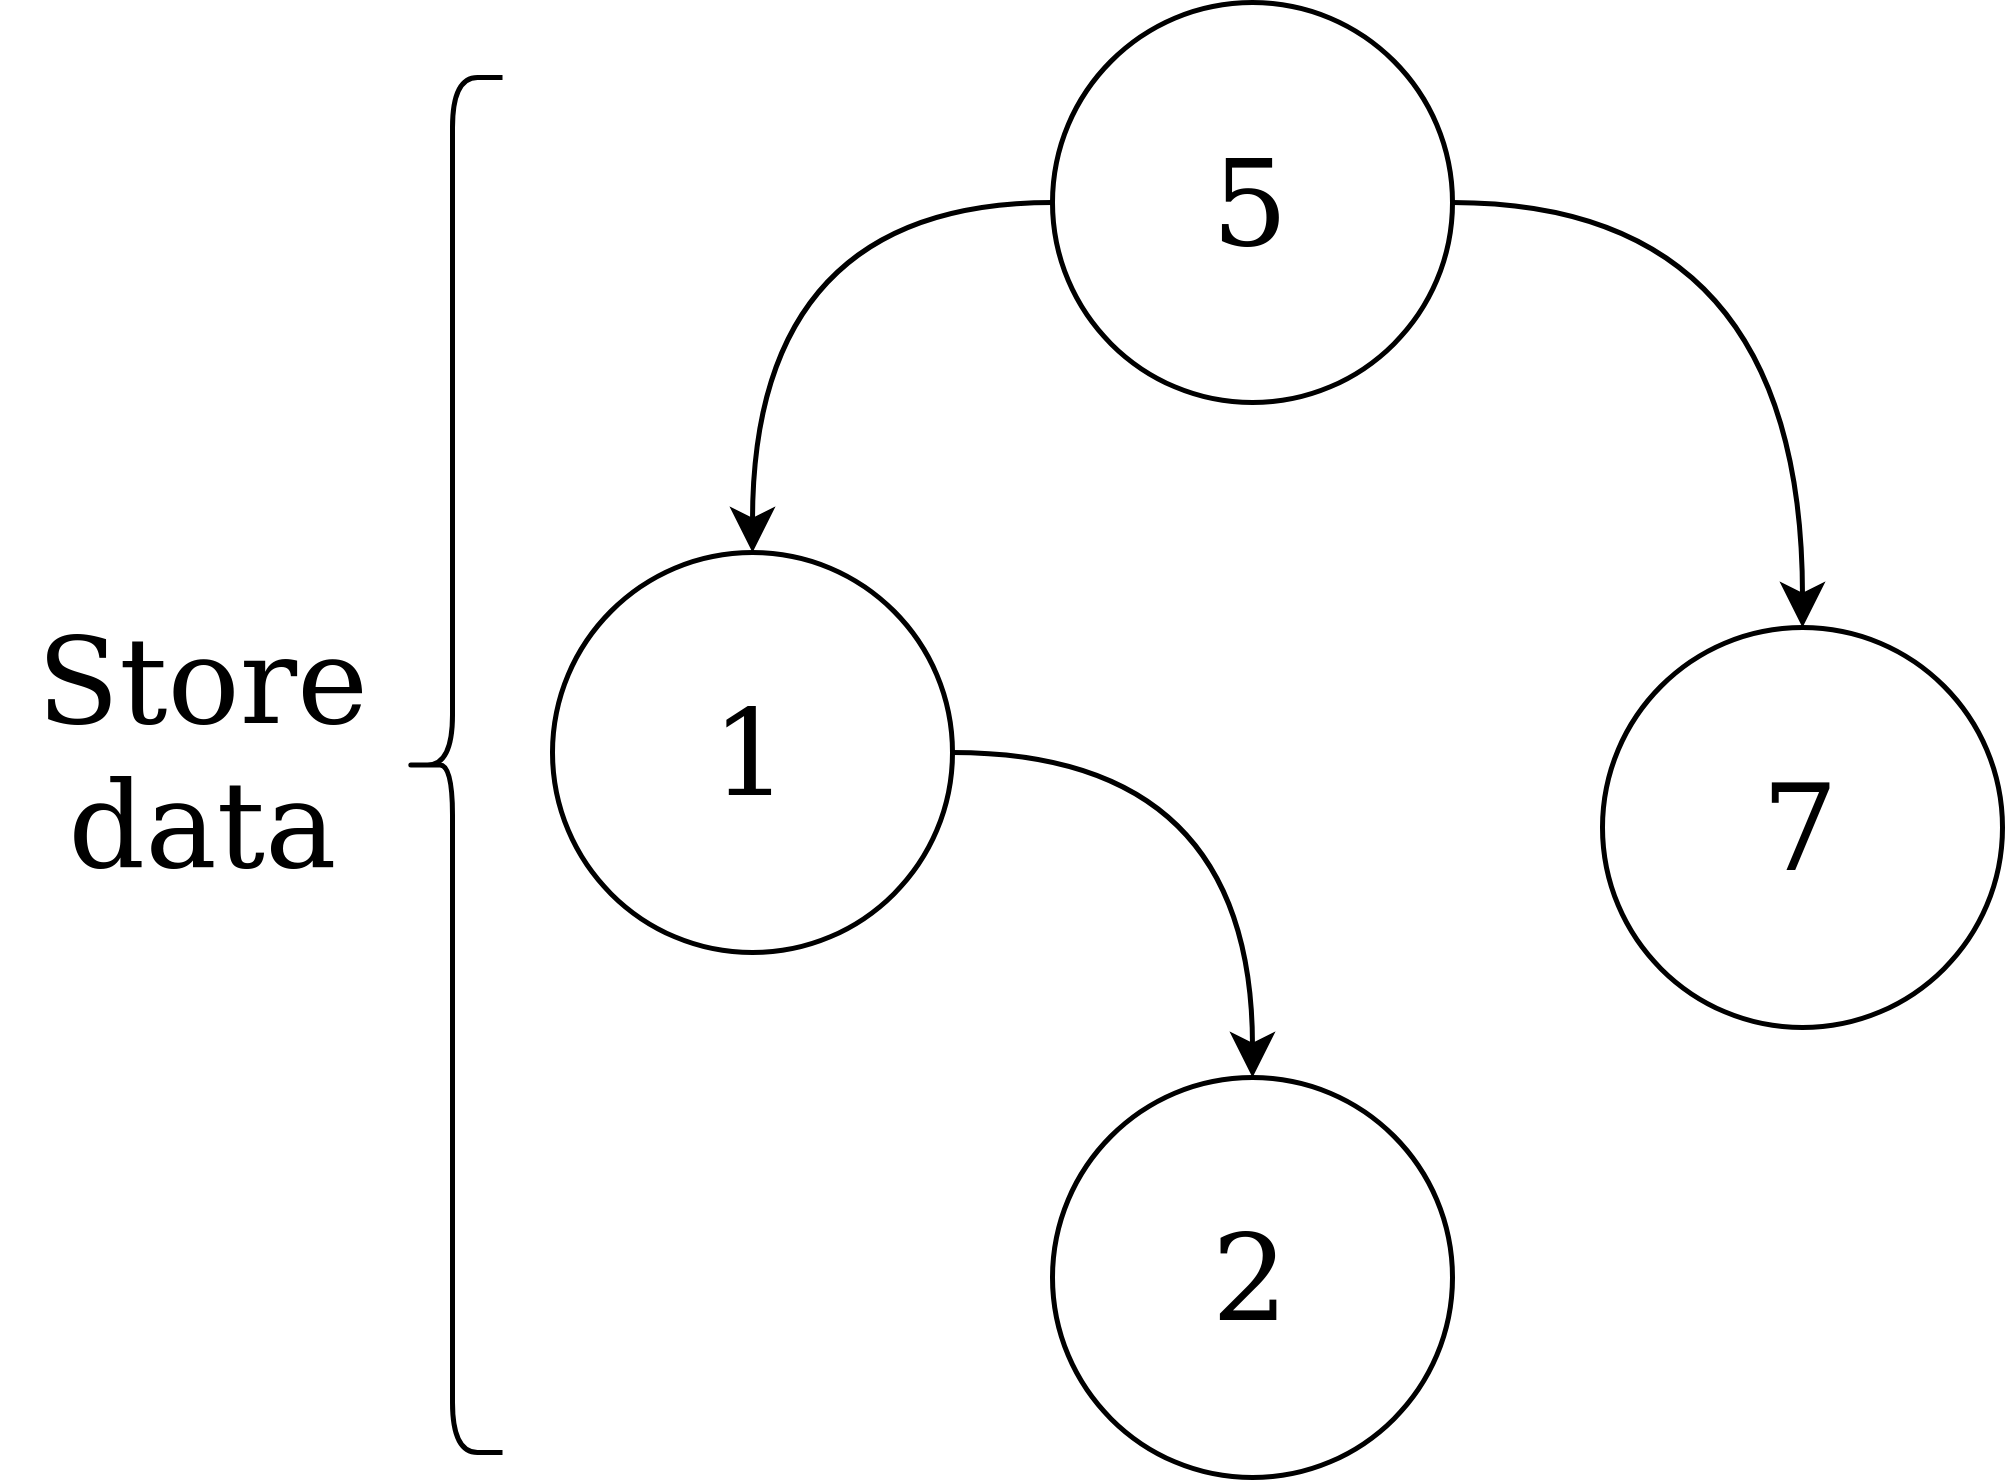
\includegraphics[width=\linewidth]{pics/internal-tree.png}
          \captionof{figure}{Internal binary search tree}
          \label{internal-tree-pic}
     \end{subfigure}
    \caption{Different types of search trees}
    \label{internal-external-trees-pic}
\end{figure}

To explain how to implement the \texttt{count} query, we consider external binary search trees. Each internal node will store \texttt{Right\_Subtree\_Min}~--- the minimal key, that might be located in the right subtree. All keys less than \texttt{Right\_Subtree\_Min} should be stored in the left subtree, and, thus, all scalar queries (\texttt{insert}, \texttt{remove} and \texttt{contains}) on such keys are redirected to the left subtree. Similarly, all keys greater than or equal to \texttt{Right\_Subtree\_Min} should be stored in the right subtree, and, thus, all scalar queries on such keys are redirected to the right subtree (Fig.~\ref{right-subtree-min-pic}).

\begin{figure}[H]
  \centering
  \caption{Using \texttt{Right\_Subtree\_Min} for query routing}
  \label{right-subtree-min-pic}
  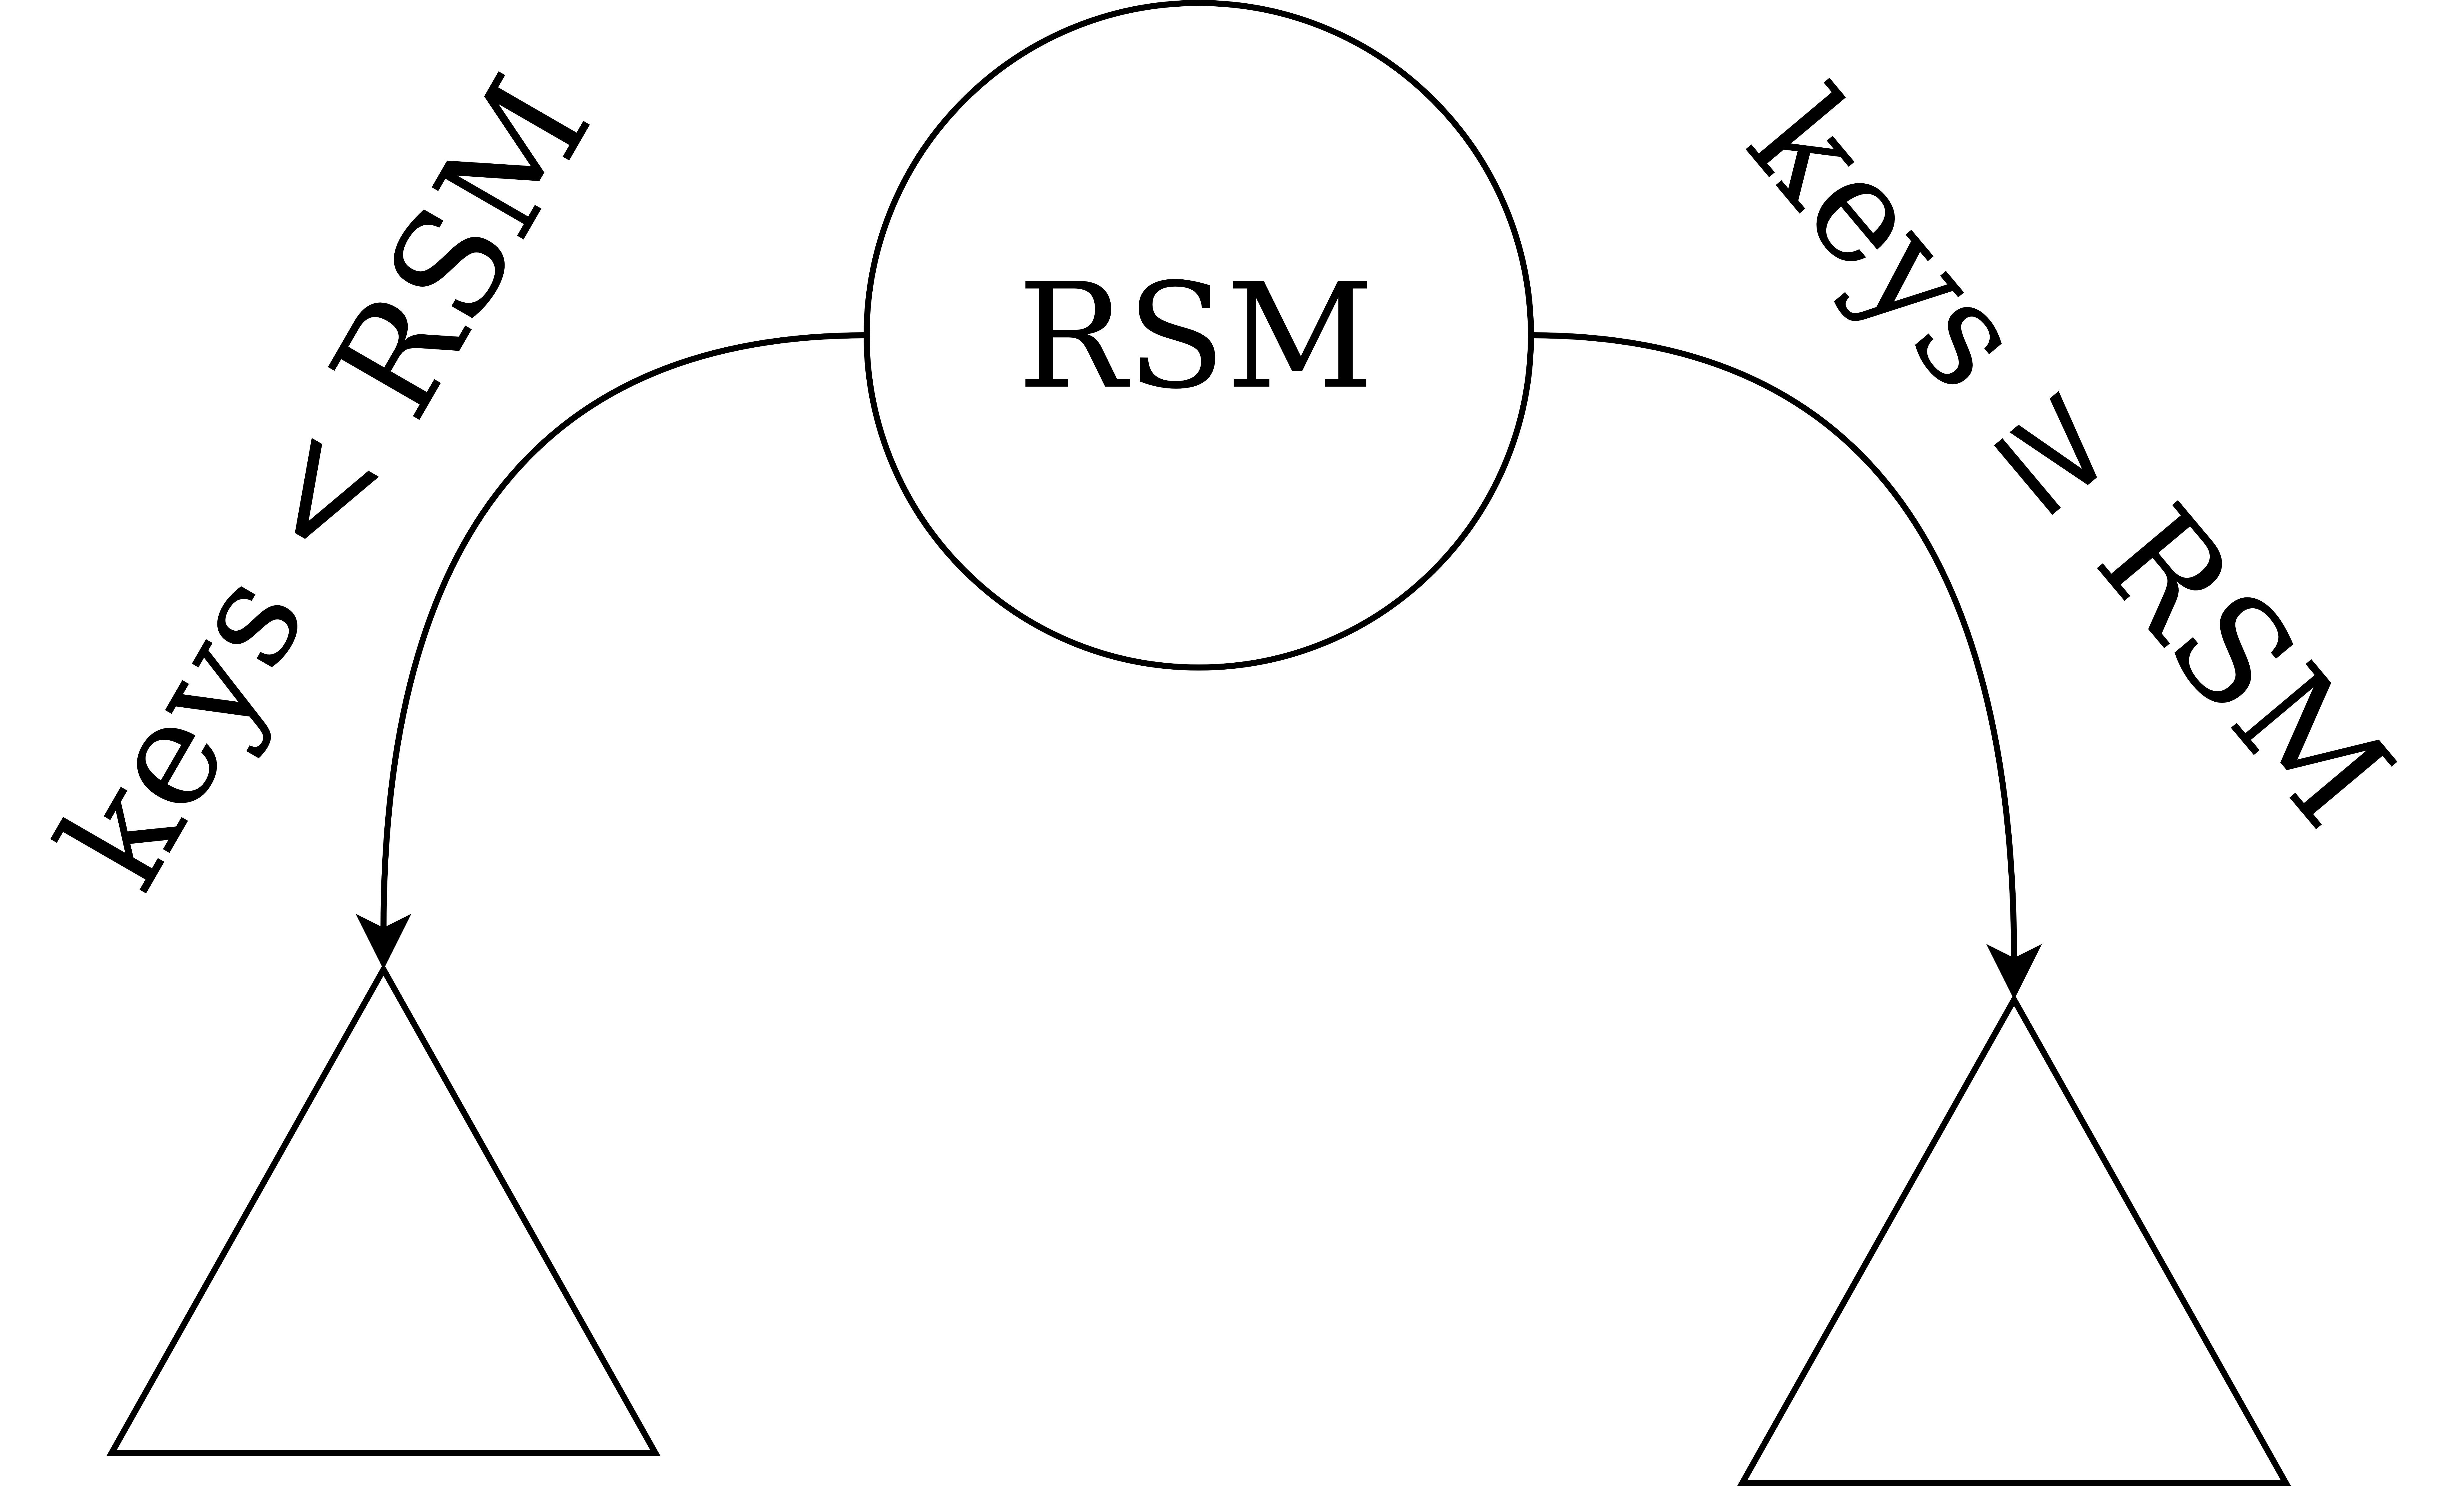
\includegraphics[width=0.5\linewidth]{pics/right_subtree_min.png}
\end{figure}

Moreover, each internal node will store the size of that node's subtree~--- i.e., the number of keys in that node's subtree. Of course, that information should be properly maintained: 
\begin{itemize}
    \item When inserting new key \texttt{k} to the tree, increase by one subtree sizes of each node on the path from the root to the leaf, storing key \texttt{k} (Fig.~\ref{insert-sizes-pic}).
    
    \item When removing key \texttt{k} from the tree, decrease by one subtree sizes of each node on the path from the root to the leaf, storing key \texttt{k} (Fig.~\ref{remove-sizes-pic}).
\end{itemize}

\begin{figure}[H]
  \centering
  \caption{Maintaining subtree sizes on node insertion}
  \label{insert-sizes-pic}
  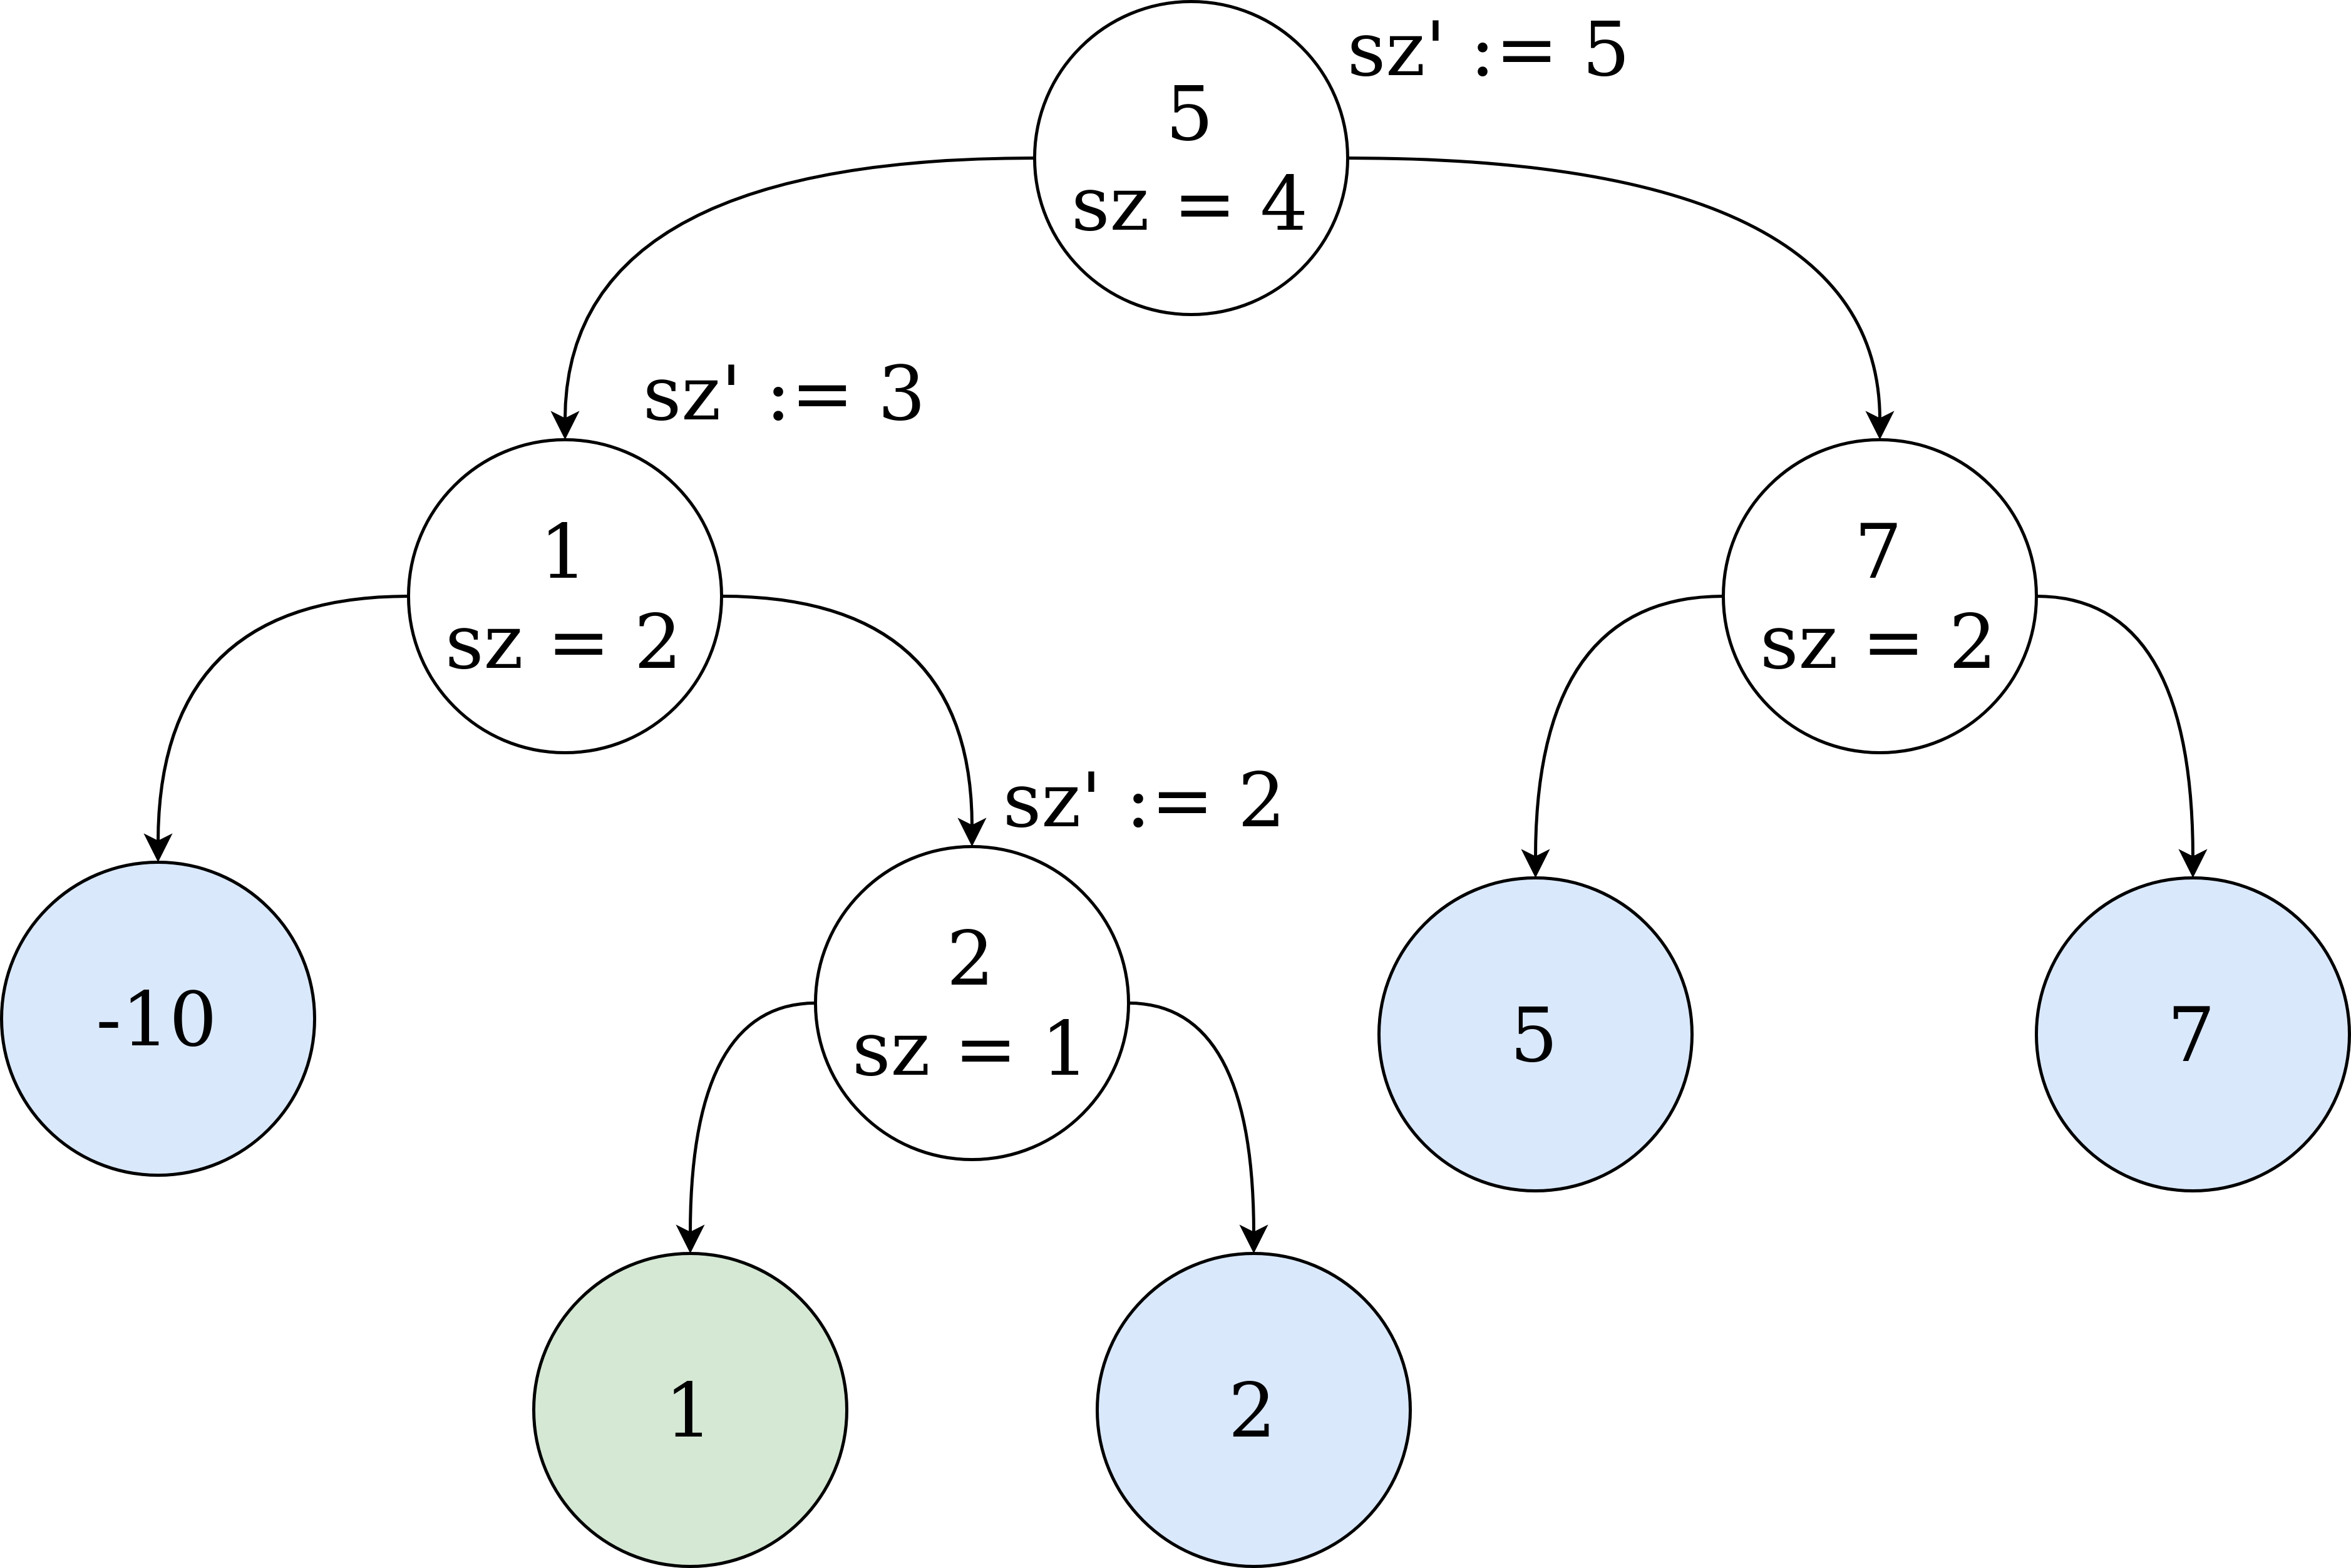
\includegraphics[width=\linewidth]{pics/insert-sizes.png}
\end{figure}

\begin{figure}[H]
  \centering
  \caption{Maintaining subtree sizes on node removal}
  \label{remove-sizes-pic}
  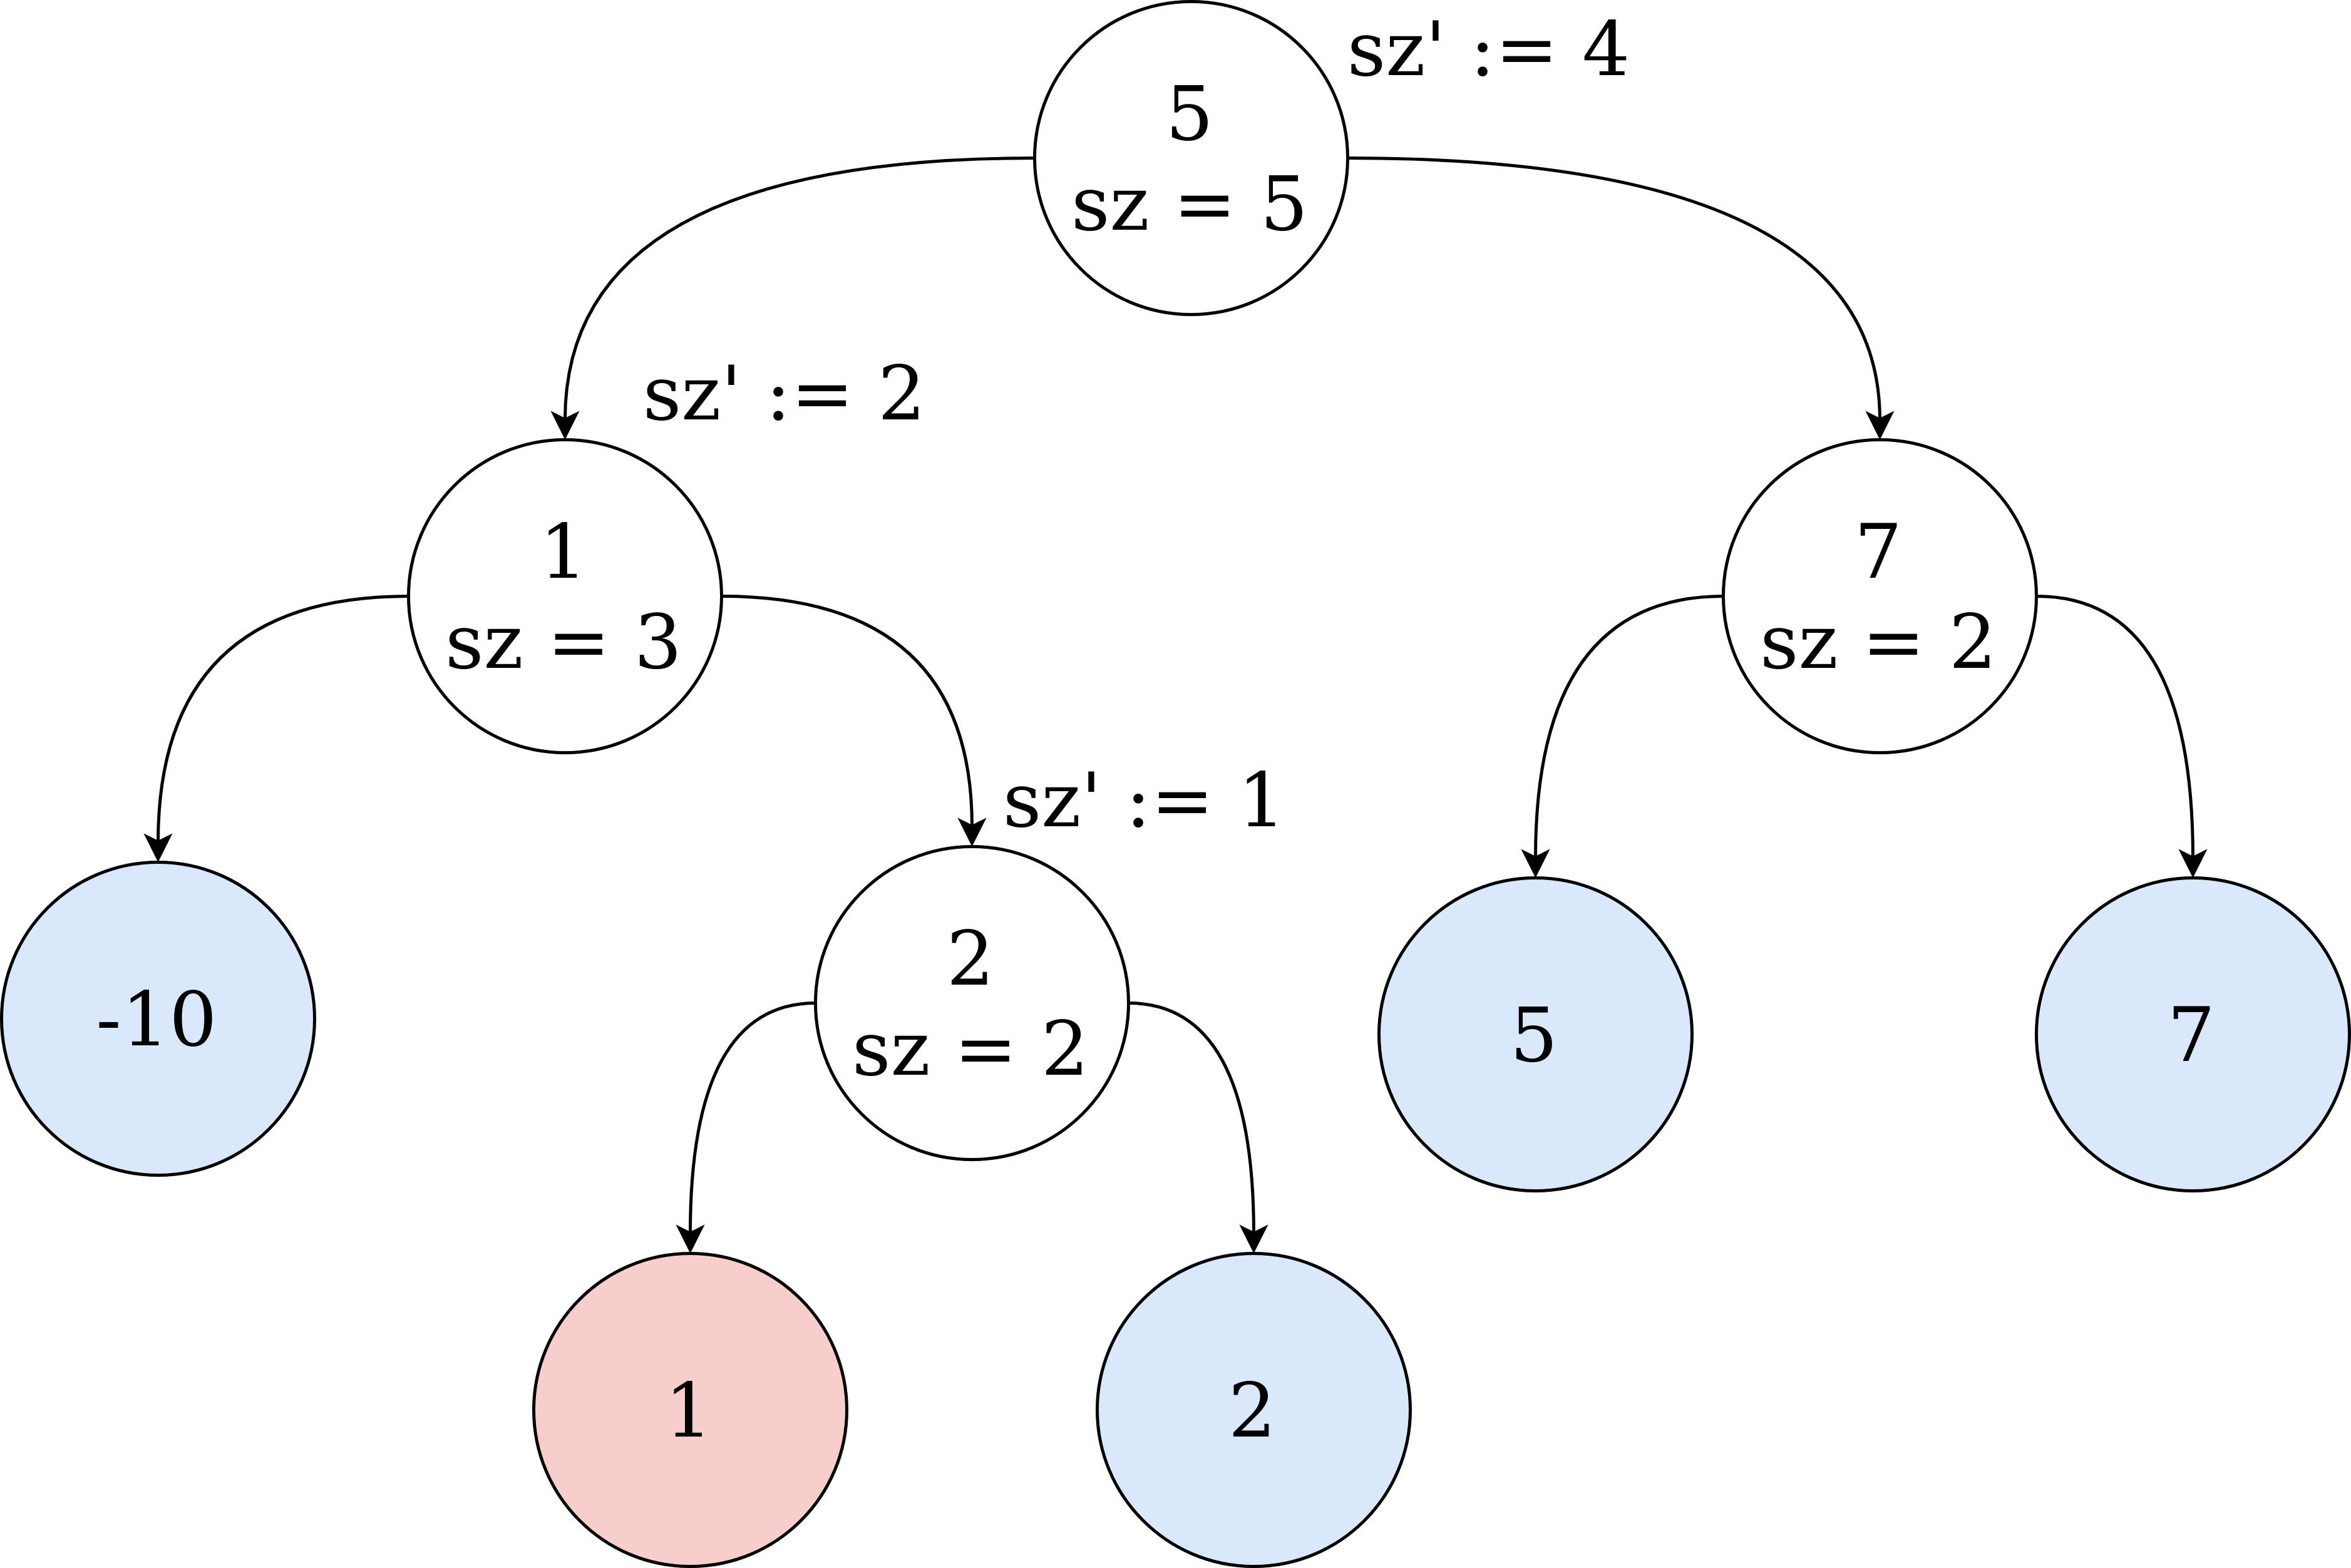
\includegraphics[width=\linewidth]{pics/remove-sizes.png}
\end{figure}

\begin{definition}
We call additional information, stored in tree nodes and required for fast range queries execution, \emph{augmentation values}.

For example, subtree sizes are augmentation values, required for asymptotically optimal execution of the \texttt{count} range query.
\end{definition}

Note, that different range queries may require different augmentations in order to be executed asymptotically optimal. In Chapter~\ref{applicability-chapter} we shall describe augmentations, required for fast execution of different range queries.

\subsection{Executing the \texttt{count} query asymptotically optimal}

To implement the \texttt{count} query in an asymptotically optimal way, we present the following three functions:

\begin{itemize}
    \item \texttt{count\_both\_borders(node, min, max)}~--- returns the number of keys in \texttt{node} subtree, that are located in the range \texttt{[min; max]}
    
    \item \texttt{count\_left\_border(node, min)}~--- returns the number of keys in \texttt{node} subtree, that are greater than or equal to \texttt{min}
    
    \item \texttt{count\_right\_border(node, max)}~--- returns the number of keys in \texttt{node} subtree, that are less than or equal to \texttt{max}
\end{itemize}

Trivially, \texttt{count(Set, min, max) = count\_both\_borders(Set.Root, min, max)}.

\bigbreak

Let us begin with defining \texttt{count\_both\_borders(node, min, max)} procedure recursively:

\begin{itemize}
    \item If \texttt{node} is a leaf, we check whether \texttt{min $\leq$ node.Key $\leq$ max} holds. If so, we return \texttt{1}, otherwise, we return \texttt{0}.

    \item If \texttt{min $\geq$ node.Right\_Subtree\_Min}, then all keys from the left subtree are less than \texttt{min} (since for all such keys \texttt{Key < node.Right\_Subtree\_Min} holds, as guaranteed by the tree structure). Thus, all the required keys are located in the right subtree. Therefore, we return \texttt{count\_both\_borders(node.Right, min, max)}.
    
    \item If \texttt{max $<$ node.Right\_Subtree\_Min}, then all keys from the right subtree are greater than \texttt{max}. Thus, all the required keys are located in the left subtree. Therefore, we return \texttt{count\_both\_borders(node.Left, min, max)}.
    
    \item Otherwise, \texttt{min $<$ node.Right\_Subtree\_Min $\leq$ max}. In that case, some satisfying keys may be located in the left subtree, and some of them may be located in the right subtree. Thus, we return \texttt{count\_both\_borders(node.Left, min, node.Right\_Subtree\_Min) + count\_both\_borders(node.Right, node.Right\_Subtree\_Min, max)}. In that case, we call \texttt{node} with such a condition a \emph{fork node}.
    
    Note, that the tree structure guarantees, that all keys in the left subtree are already less than \texttt{node.Right\_Subtree\_Min} and all keys in the right subtree are already greater than or equal to \texttt{node.Right\_Subtree\_Min}. Thus, we do not need to check, that keys in the left subtree are $\leq$ \texttt{node.Right\_Subtree\_Min} and that keys in the right subtree are $\geq$ \texttt{node.Right\_Subtree\_Min}~--- these inequations are guaranteed to be true by the tree structure itself. Thus, we return \texttt{count\_left\_border(node.Left, min) + count\_right\_borders(node.Right, max)}.
\end{itemize}

\bigbreak

Now, we shall define \texttt{count\_left\_border(node, min)}:

\begin{itemize}
    \item If \texttt{node} is a leaf, we check whether \texttt{node.Key $\geq$ min} holds. If so, we return \texttt{1}, otherwise, we return \texttt{0}.
    
    \item If \texttt{min $\geq$ node.Right\_Subtree\_Min}, then all keys from the left subtree are less than \texttt{min}. Thus, all the required keys are located in the right subtree. Therefore, we return \texttt{count\_left\_border(node.Right, min)}.
    
    \item Otherwise, \texttt{min $<$ node.Right\_Subtree\_Min}. In that case, all the keys from the right subtree are greater than or equal to \texttt{min}. Thus, we should count all keys from the right subtree plus some keys from the left subtree. Therefore, the answer is \texttt{get\_size(node.Right) + count\_left\_border(node.Left, min)}.
    
    Size of the right subtree can be calculated easily:
    
    \begin{itemize}
        \item If \texttt{node.Right} is a leaf, the size of the right subtree is \texttt{1};
        
        \item Otherwise, \texttt{node.Right} is an internal node~--- in that case the size of the right subtree is \texttt{node.Right.Size};
    \end{itemize}
\end{itemize}

\bigbreak

We can define \texttt{count\_right\_border(node, max)} in the same manner:

\begin{itemize}
    \item If \texttt{node} is a leaf, we check whether \texttt{node.Key $\leq$ max} holds. If so, we return \texttt{1}, otherwise, we return \texttt{0}.
    
    \item If \texttt{max $<$ node.Right\_Subtree\_Min}, then all keys from the right subtree are greater than \texttt{max}. Thus, all the required keys are located in the left subtree. Therefore, we return \texttt{count\_right\_border(node.Left, max)}.
    
    \item Otherwise, \texttt{max $\geq$ node.Right\_Subtree\_Min}. In that case, all keys from the left subtree are less than \texttt{max}. Thus, we should count all keys from the left subtree plus some keys from the right subtree. Therefore, the answer is \texttt{get\_size(node.Left) + count\_right\_border(node.Right, max)}. The size of the left subtree can be calculated similarly to the previous case.
\end{itemize}

\bigbreak

We show how to implement the algorithm in Listing~\ref{count-sequential-listing} \footnote{In all subsequent pseudocode listings we denote shared objects (including names of fields, that may be accessed by multiple processes) in \texttt{Upper\_Snake\_Case}; class names in \texttt{CamelCase}; local variables in \texttt{lower\_snake\_case}; functions in \texttt{lower\_snake\_case}; Creation of a new variable is denoted by \texttt{variable\_name := initial\_value} syntax; Assigning a new value to the existing variable is denoted by \texttt{variable\_name $\leftarrow$ new\_value} syntax;}.

\renewcommand{\lstlistingname}{Listing}
\begin{lstlisting}[caption={Implementation of the \texttt{count} range query},label={count-sequential-listing},escapeinside={(*}{*)}, captionpos=b]
fun count_both_borders(node, min, max):
    case node of
    | EmptyNode (*$\rightarrow$*)
        /* 
        EmptyNode is a dummy node that contains neither key nor children.
        We can use it to represent an empty set, for example
        */
        return 0
    | LeafNode (*$\rightarrow$*)
        if min (*$\leq$*) node.Key (*$\leq$*) max:
            return 1
        else:
            return 0
    | InnerNode (*$\rightarrow$*)
        if min (*$\geq$*) node.Right_Subtree_Min:
            return count_both_borders(mode.Right, min, max)
        elif max < node.Right_Subtree_Min:
            return count_both_borders(node.Left, min, max)
        else:
            return count_left_border(node.Left, min) +
                   count_right_border(node.Right, max)
    
fun get_size(node):
    case node of
    | EmptyNode (*$\rightarrow$*)
        return 0    
    | LeafNode (*$\rightarrow$*)
        return 1
    | InnerNode (*$\rightarrow$*)
        return node.Size   
                   
fun count_left_border(node, min):
    case node of
    | EmptyNode (*$\rightarrow$*)
        return 0
    | LeafNode (*$\rightarrow$*)
        if node.Key (*$\geq$*) min:
            return 1
        else:
            return 0
    | InnerNode (*$\rightarrow$*)
        if min (*$\geq$*) node.Right_Subtree_Min:
            return count_left_border(node.Right, min)
        else:
            return get_size(node.Right) + 
                   count_left_border(node.Left, min)
            
fun count_right_border(node, max):
    case node of
    | EmptyNode (*$\rightarrow$*)
        return 0
    | LeafNode (*$\rightarrow$*)
        if node.Key (*$\leq$*) max:
            return 1
        else:
            return 0
    | InnerNode (*$\rightarrow$*)
        if max < node.Right_Subtree_Min:
            return count_right_border(node.Left, max)
        else:
            return get_size(node.Left) + 
                   count_right_border(node.Right, max)
\end{lstlisting}

\subsection{Time complexity analysis}

\begin{theorem}
The time complexity of the \texttt{count} query is $O(height)$.
\end{theorem}
\begin{proof}
We state that both \texttt{count\_left\_border} and \texttt{count\_right\_border} work in $O(height)$ time. Indeed, on each tree level both these procedures visit only one node per level, performing $O(1)$ operations in each visited node.

Let us now switch to proving the time complexity of \texttt{count\_both\_borders}. At upper tree levels (higher than the \emph{fork node}) it visits one node per level performing $O(1)$ operations in each visited node, giving $O(height)$ time at upper levels. 

At one of the nodes (the \emph{fork node}) the execution may fork: we shall call \texttt{count\_left\_border} on the left subtree and \texttt{count\_right\_border} on the right subtree. Note, that the execution can fork at most once and both called procedures have $O(height)$ time complexity. Thus, at lower tree levels the procedure also has $O(height) + O(height) = O(height)$ time complexity. Therefore, the total time complexity of the procedure is $O(height)$ (Fig~\ref{sequential-time-png}).

\begin{figure}[H]
  \centering
  \caption{Time complexity of the \texttt{count\_both\_borders} procedure}
  \label{sequential-time-png}
  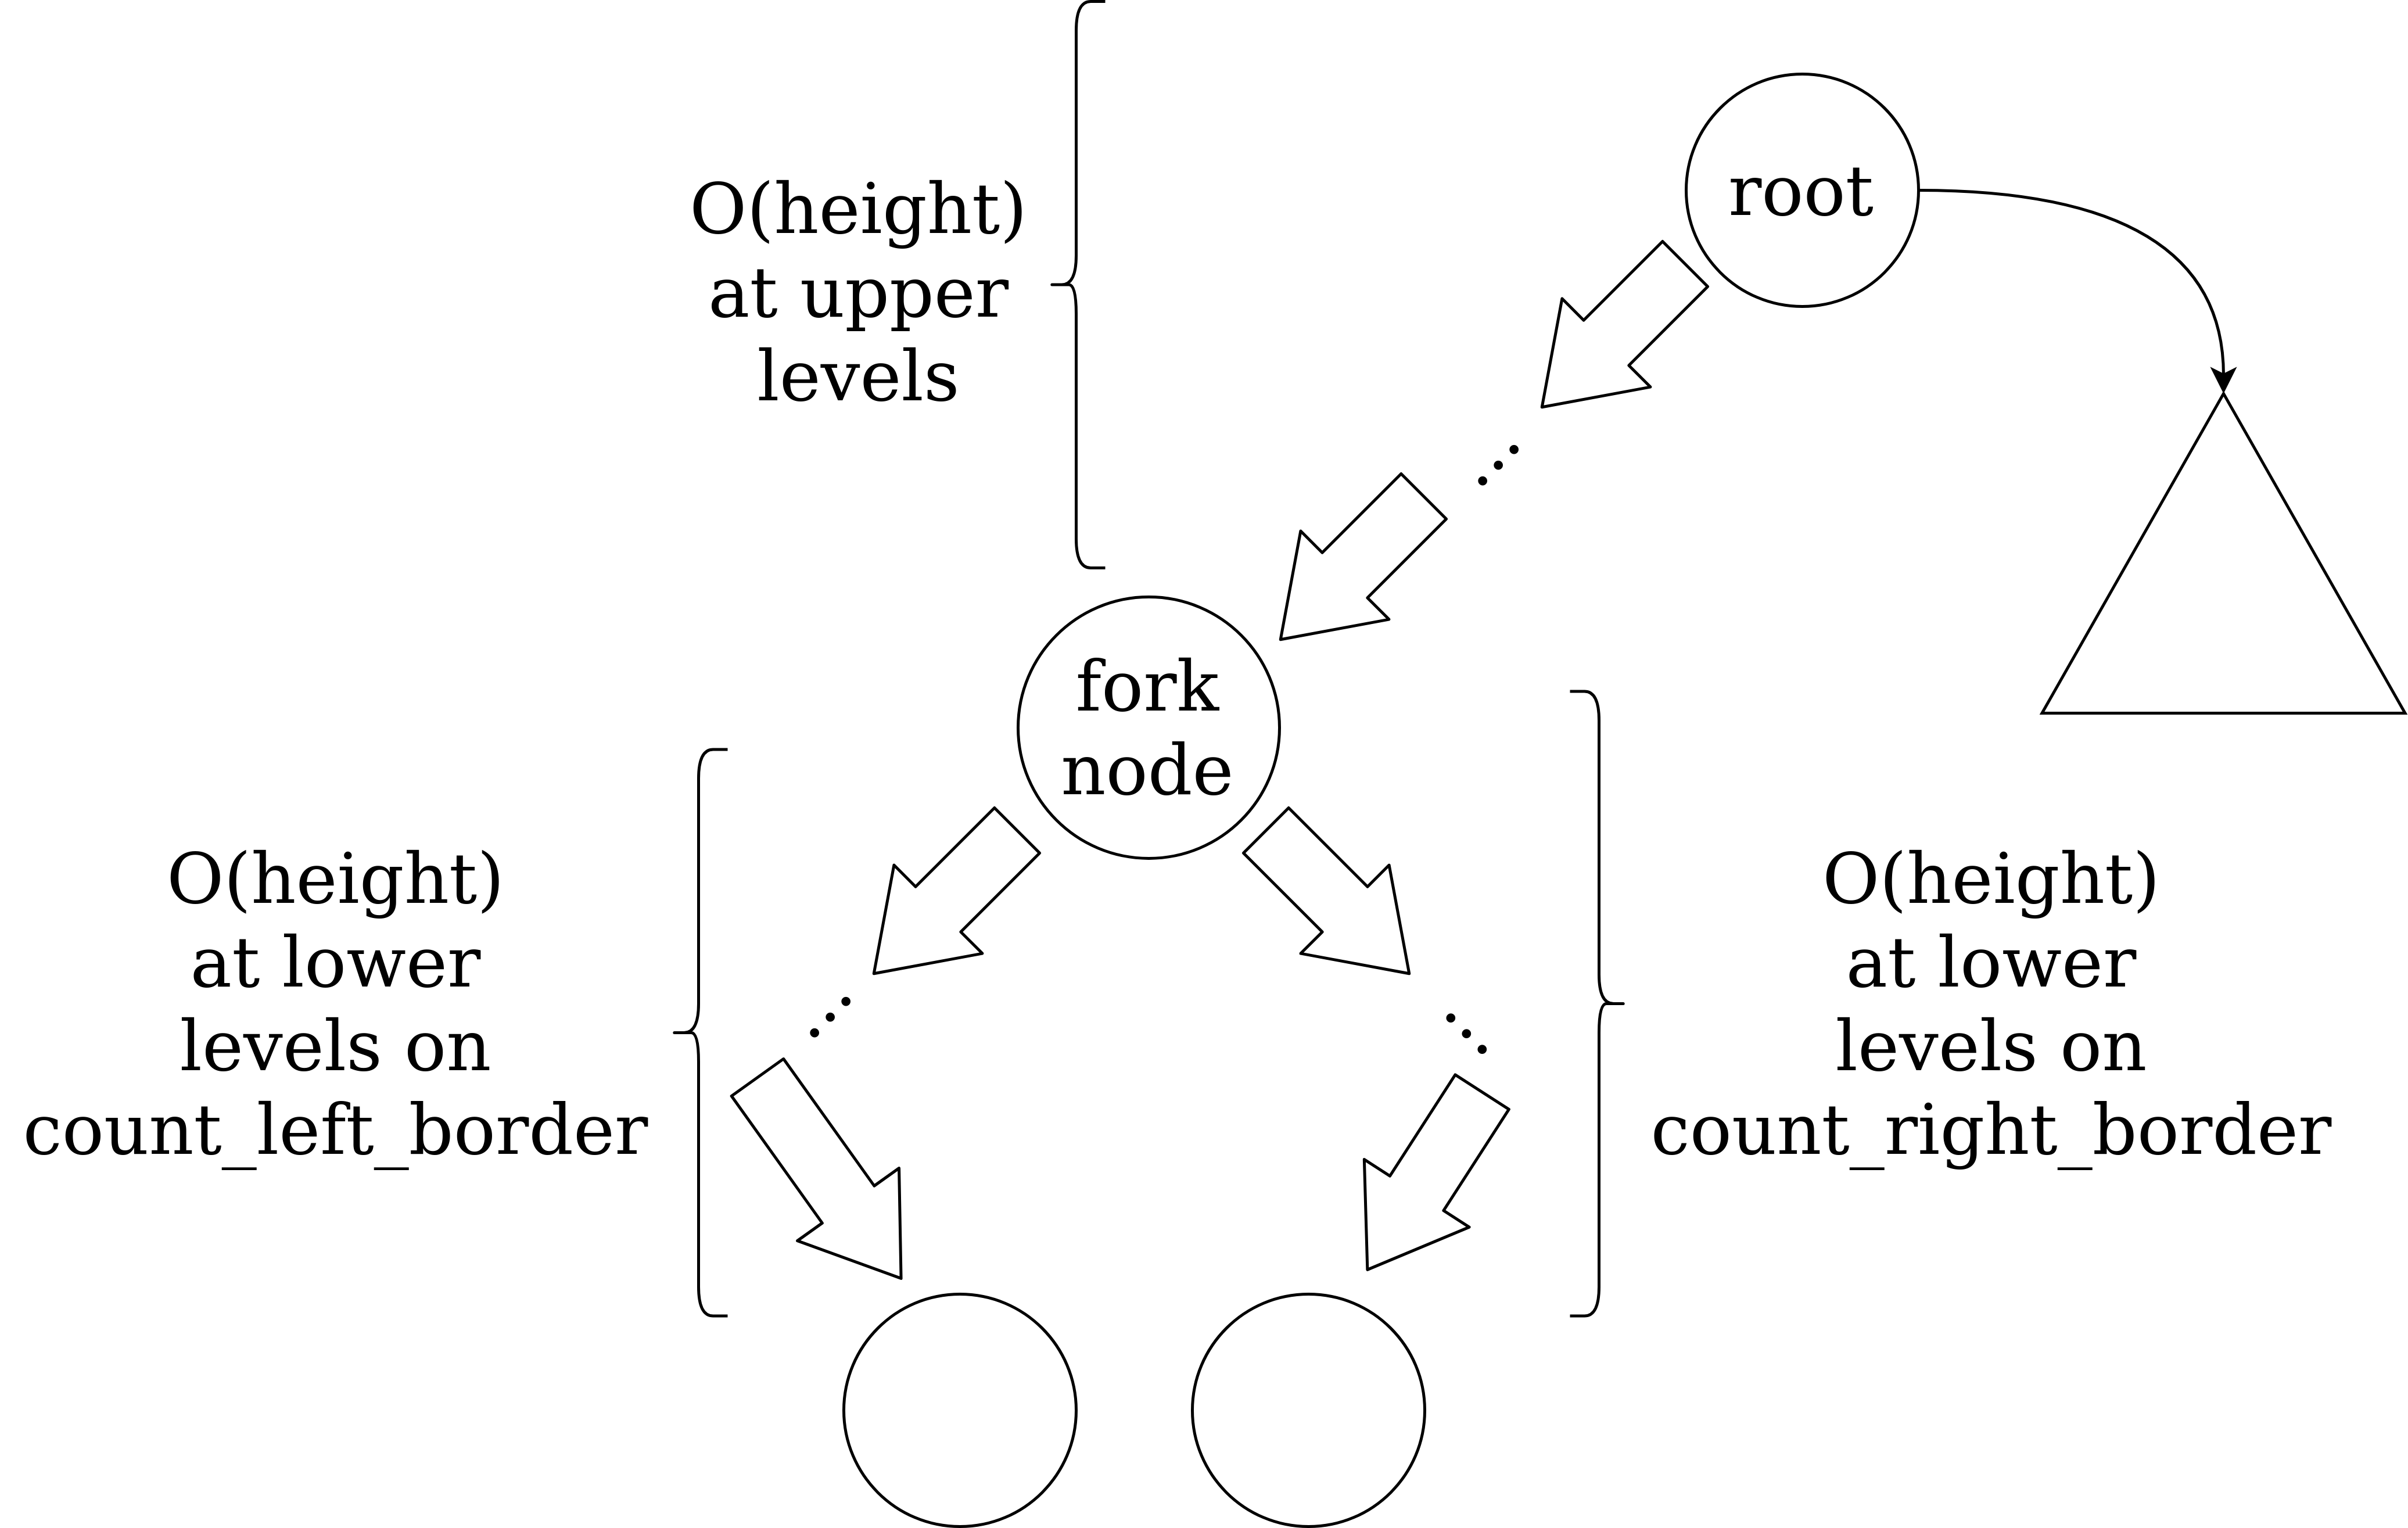
\includegraphics[width=\linewidth]{pics/sequential-time.png}
\end{figure}
\end{proof}

Suppose we use balanced binary search trees with $height \in O(\log N)$ where $N$ is the size of the tree. Thus, the \texttt{count} query is executed in $O(\log N)$ time.

\section{Range queries applications}

\subsection{Spammers identification}

Suppose we are developing a database for a messenger. In that case, SQL definition of a table, that will store sent messages might look like this (Listing~\ref{messages-definition-listing}):

\renewcommand{\lstlistingname}{Listing}
\begin{lstlisting}[caption={SQL definition of the \texttt{Messages} table},label={messages-definition-listing},language=SQL,escapeinside={(*}{*)},captionpos=b]
CREATE TABLE Messages
(
    sender_id INT,
    receiver_id INT,
    send_timestamp TIMESTAMP,
    message_text VARCHAR
);
\end{lstlisting}

Suppose also, that we want to identify spammers, given that database. One possible approach is to find users, that send a lot of messages during a short time period. To implement that approach, we should be able to answer a certain query: how many messages has some particular user sent during some particular time period? When written in SQL, that query might look like this (Listing~\ref{sql-count-listing}):

\renewcommand{\lstlistingname}{Listing}
\begin{lstlisting}[caption={SQL query for getting the number of messages, sent by a particular user during a particular time period},label={sql-count-listing},language=SQL,captionpos=b]
SELECT COUNT(*)
FROM Messages
WHERE sender_id = :s_id AND 
      send_timestamp BETWEEN :start_ts AND :start_ts + :time_delta
\end{lstlisting}

How can such queries be answered fast? We can build an ordered index on fields \texttt{(sender\_id, send\_timestamp)} (Fig.~\ref{SQL-index}).

\begin{figure}[H]
  \centering
  \caption{Binary search tree (BST) as an ordered index on fields \texttt{(sender\_id, send\_timestamp)}}
  \label{SQL-index}
  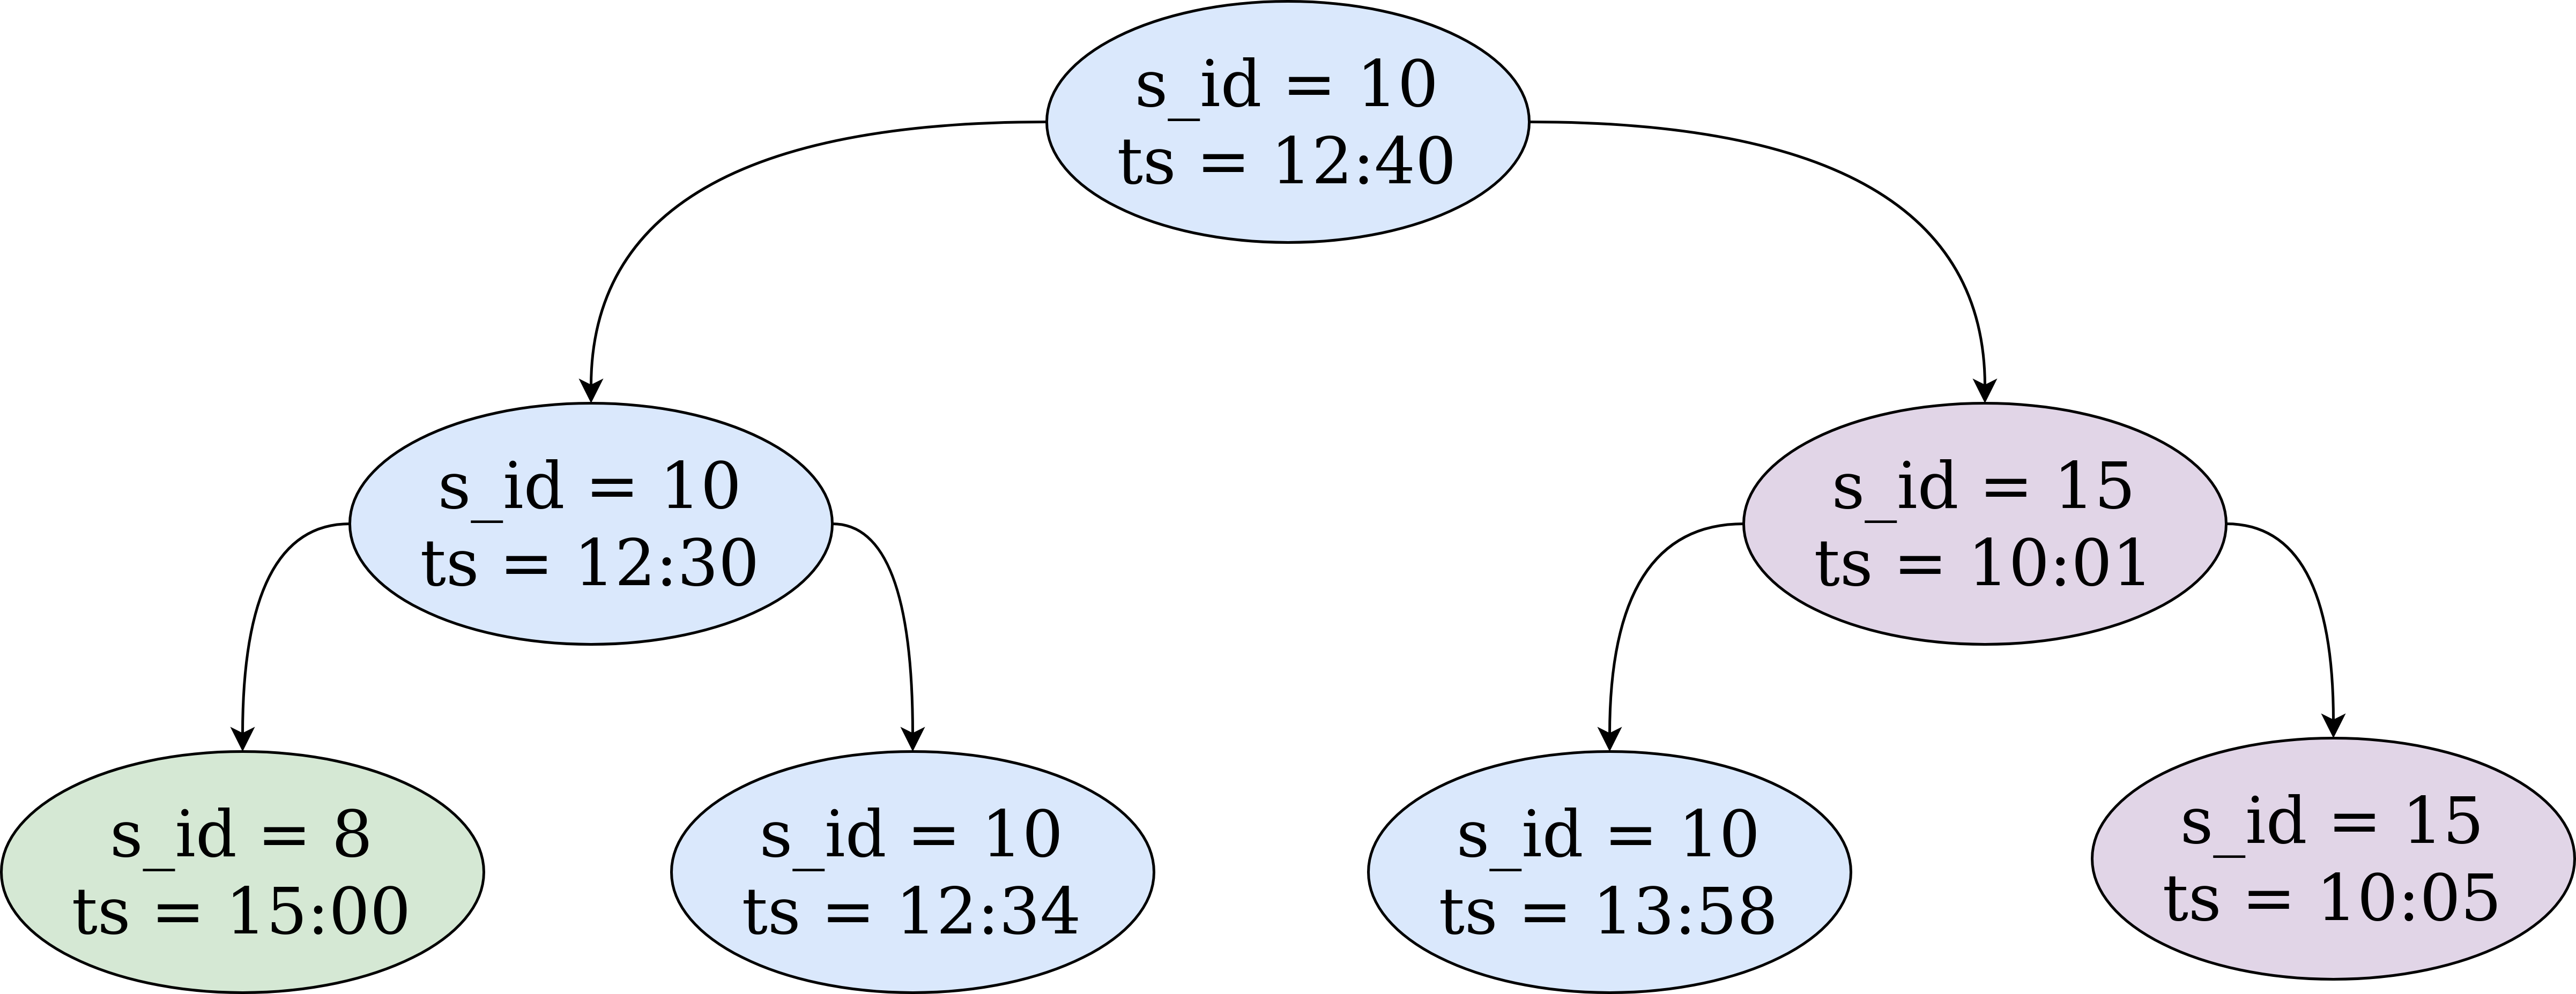
\includegraphics[width=\linewidth]{pics/sql-index.png}
\end{figure}

In such case, executing such SQL queries can be reduced to executing a range query \texttt{count(min = (:s\_id, :start\_ts), max = (:s\_id, :start\_ts + :time\_delta))} on a binary search tree, serving as an ordered index. In that case, the faster the BST can process such queries, the faster we can identify spammers. Thus, we need our index implementation to process such range queries in an asymptotically optimal manner.

\subsection{Traffic jams identification}

Suppose we are building an application, that should identify traffic jams based on a car location information and warn drivers to change their route, if it is expected to go through a traffic jam. In such case, a crucial part of our application would be an algorithm, that can identify traffic jams very fast.

But what is a traffic jam? To a first approximation it is a small area, that contains an enormous number of cars. Thus, to identify traffic jams, we must be able to answer a certain query: how many cars are located in the specified area? Assuming a car is a point on a plane and a search area is a rectangle (Fig.~\ref{cars-area}), we can solve this task using range queries on R-trees~\cite{guttman1984r} or k-d trees~\cite{de2000computational}. Therefore, once again, we need our R-tree or k-d tree implementation to process such range queries in an asymptotically optimal manner.

\begin{figure}[H]
  \centering
  \caption{Traffic jams identification problem}
  \label{cars-area}
  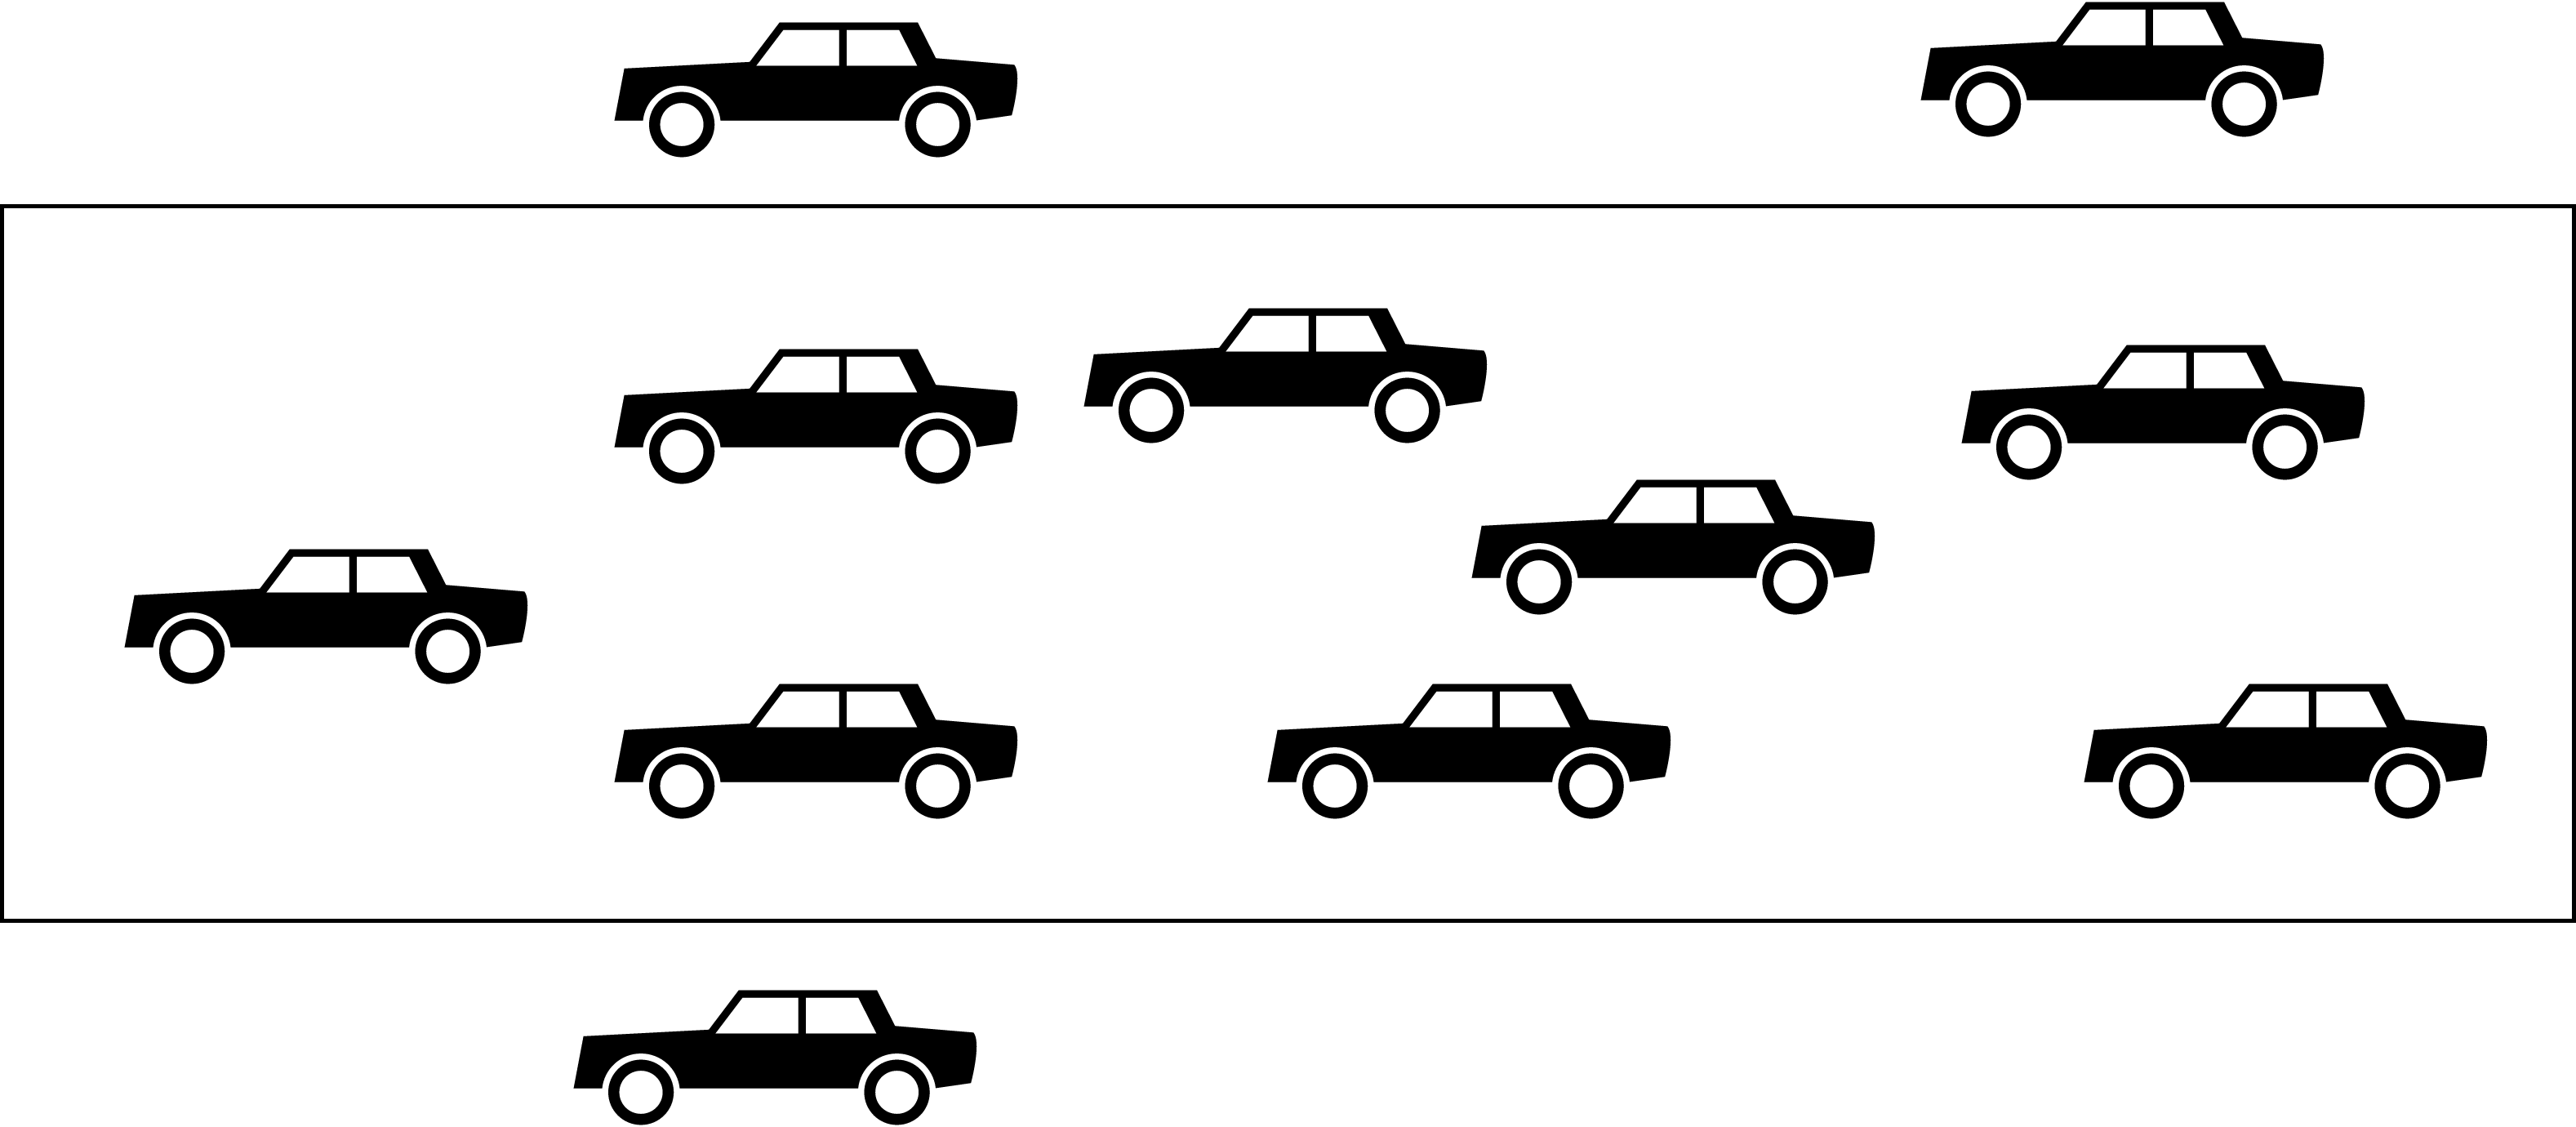
\includegraphics[width=\linewidth]{pics/cars-area.png}
\end{figure}

Thus, as can be seen, in both above-described cases the quality of our application directly depends on our ability to perform efficient range queries on trees.

\section{Execution model}

We consider the standard concurrent system model with a set of \texttt{n} processes \footnote{Hereinafter terms ``process'' and ``thread'' are used interchangeably: in the context of this work they mean the same.} $\{\texttt{p}_{\texttt{i}}\}_{i = 1}^n$ that work asynchronously and each of which executes its own sequence of operations.

Process communicate with each other by executing operations on objects, located in the shared memory. Basic shared objects (called \emph{registers}) provide atomic \texttt{read/write} operations. Moreover, they can provide atomic \texttt{read-modify-write} operations, like \texttt{compare-and-swap} \cite{compare-and-swap}, \texttt{fetch-and-add} \cite{fetch-and-add}, \texttt{test-and-set} \cite{test-and-set}.

Amongst all \texttt{read-modify-write} operations, the most relevant for us is \texttt{compare-and-swap} (or \texttt{compare-and-set}, or \texttt{CAS}). This operation has three arguments: register, the expected value and the new value. \texttt{CAS} atomically checks, whether the value of the register equals to the expected value. If so, \texttt{CAS} sets the value of the register equal to the new value and returns \texttt{true}. Otherwise, it lefts the register value unmodified and returns \texttt{false}. The \texttt{CAS} operation can be specified in the following pseudocode (Listing~\ref{cas-listing}):

\renewcommand{\lstlistingname}{Listing}
\begin{lstlisting}[caption={Pseudocode for the \texttt{CAS} operation},label={cas-listing},escapeinside={(*}{*)}, captionpos=b]
fun cas(Register, expected_value, new_value):
    atomically:
        cur_value := Register
        if cur_value = expected_value:
            Register (*$\leftarrow$*) new_value
            return true
        else:
            return false
\end{lstlisting}

We can use basic shared objects to build more complex shared objects, representing different concurrent data structures. For example, we can use a collection of \texttt{read/write/CAS} registers to build a concurrent queue~\cite{michael1996simple} or stack~\cite{treiber1986systems}.

Moreover, each process $\texttt{p}_{\texttt{i}}$ has access to an arbitrary set of local objects, on which only $\texttt{p}_{\texttt{i}}$ can execute operations. If an object $\texttt{Obj}$ is local to process $\texttt{p}_{\texttt{i}}$, only the process $\texttt{p}_{\texttt{i}}$ has access to it and can execute operations on $\texttt{Obj}$ (Fig.~\ref{model-pic}).

\begin{figure}[H]
  \centering
  \caption{Concurrent system model}
  \label{model-pic}
  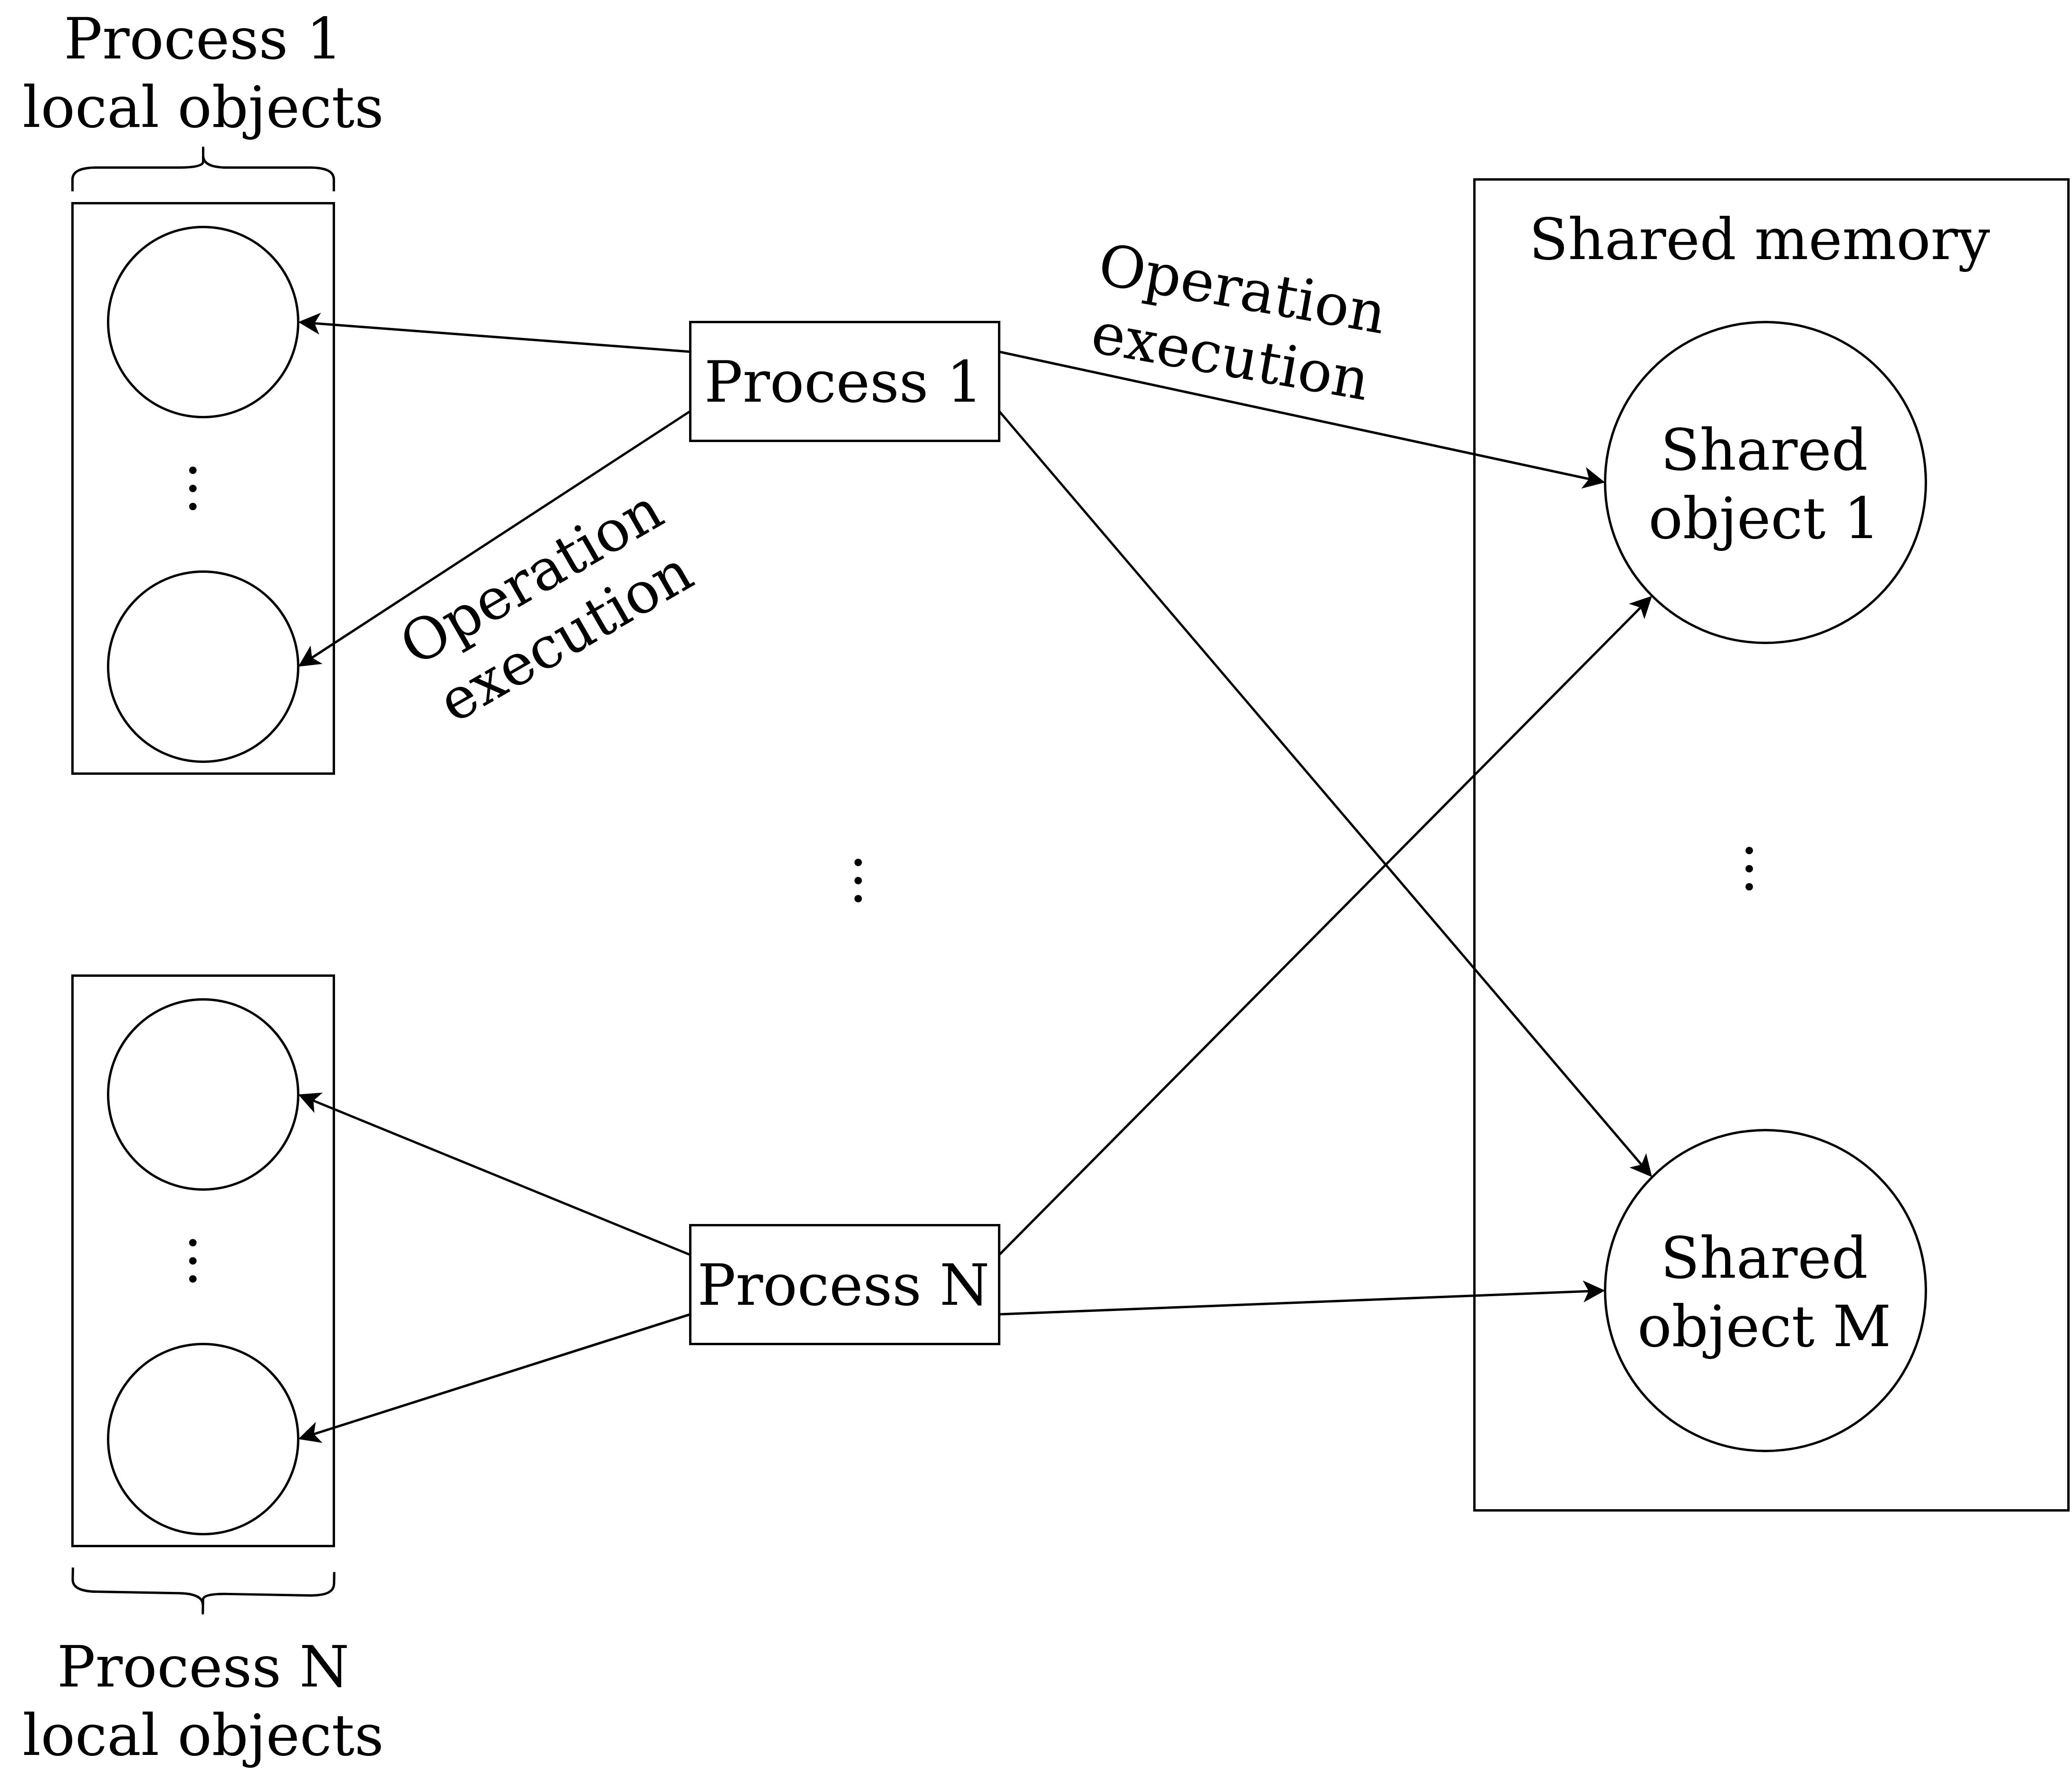
\includegraphics[width=\linewidth]{pics/model.png}
\end{figure}

We assume that the processes work asynchronously, each with its own speed, without synchronizing neither their pace nor the number of operations executed. Moreover, each process can be suspended indefinitely by the underlying (e.g., OS) scheduler.

\section{Concurrent correctness criteria}
\label{correctness-criteria-section}

Consider an execution of a program, where two operations: \texttt{Set.insert(5)} and \texttt{Set.contains(5)} are performed concurrently. Suppose the former request returns \texttt{true} (i.e., \texttt{5} was inserted to the set) and the latter request returns \texttt{false} (i.e. \texttt{5} did not exist in the set). How can one tell, whether the code works correctly or not?

More formally, consider a concurrent implementation of a data type $T$. We want to have a correctness criteria, that will tell us, whether this concurrent implementation is correct (in some sense) or not. 

Before we can get to the formulation of correctness criteria, we should give additional definitions.

\bigbreak

\begin{definition}
A \emph{low-level history} (or an \emph{execution}) is a finite or infinite sequence of primitive steps: invocations and responses of high-level operations, invocations and responses of primitives on the shared registers (reads, writes, etc.). We assume that executions are \emph{well-formed}: no process invokes a new primitive, or high-level operation before the previous primitive, or a high-level operation, respectively, returns or takes steps outside its operation’s interval.
\end{definition}

\begin{definition}
A \emph{high-level history} (or simply a \emph{history}) of execution $\alpha$ on high-level object $O$ is the
subsequence of $\alpha$ consisting of all invocations and responses of operations on $O$.
\end{definition}

\begin{definition}
Two high-level histories $H$ and $L$ are considered \emph{equivalent} iff three conditions are met:
\begin{itemize}
    \item They are defined on the same object $O$;
    \item $H$ and $L$ consists of the same set of operations;
    \item All operations in $L$ have the same input and the same output as the corresponding operations in $H$;
\end{itemize}
\end{definition}

\bigbreak
\begin{definition}
High-level history $L$ is said to be \emph{sequential} if for any two operations $o_1, o_2 \in L$ either $o_1$ precedes $o_2$ or vice-versa, i.e. there are no concurrent operations in $L$.
\end{definition}

\bigbreak
Multiple correctness conditions for concurrent executions exist. We outline some of them, from the least to the most strict.

\begin{itemize}
    \item \emph{Serializability}, described in~\cite{papadimitriou1979serializability,spanner-serializability}. History $H$ is said to be serializable iff there exists sequential history $L$, equivalent to $H$. As can be seen from the definition, operations in $H$ can be reordered arbitrary, we only care about the equivalence of operation results.
    
    A concurrent implementation of a data type is \emph{serializable} iff each of its possible histories is \emph{serializable}.
    
    \item \emph{Sequential consistency}, described in~\cite{lamport1979make}. To reason about the notion of sequential consistency, we should consider a set of processes $\{p_i\}_{i = 1}^n$, executing operations from history $H$. 
    
    History $H$ is said to be sequentially consistent iff there exists a sequential history $L$, equivalent to the history $H$. Moreover, history $L$ should satisfy one additional requirement: if operations $o_1$ and $o_2$ were executed by the same process $p_i$ in $H$ and $o_1$ was executed before $o_2$ \footnote{Note, that for each pair $(o_1, o_2)$ of operations, executed by a single process $p_i$, either $o_1$ precedes $o_2$ or vise-versa, since a single process always has sequential behaviour, even in a concurrent environment}, $o_1$ should precede $o_2$ in $L$.
    
    As follows from the definition, each sequentially consistent history is serializable, since serializability only requires that an equivalent sequential history $L$ exists, while sequential consistency places additional requirements on $L$.
    
    A concurrent implementation of a data type is \emph{sequentially consistent} iff each of its possible histories is \emph{sequentially consistent}.
    
    \item \emph{Linearizability}, described in~\cite{herlihy1990linearizability}. To reason about the notion of linearizability, we should consider $\rightarrow_H$ (pronounced \emph{happens-before}): partial order on operations from a concurrent history $H$. We say, that $o_1 \rightarrow_H o_2 \mid o_1, o_2, \in H$ (pronounced $o_1$ \emph{happens-before} $o_2$) if $o_1$ is completed before $o_2$ begins. Such operations can be causally related, i.e., $o_1$ can be a cause of $o_2$. If operations $o_1$ and $o_2$ are executed by the same process $p_i$ and $o_1$ precedes $o_2$ in $p_i$ execution, $o_1 \rightarrow_H o_2$. The \emph{happens-before} relation is discussed more formally in~\cite{lamport2019time}.
    
    History $H$ is said to be linearizable iff there exists a sequential history $L$, equivalent to the history $H$. Moreover, execution $L$ should satisfy one additional requirement: if $o_1 \rightarrow_H o_2$, $o_1$ should precede $o_2$ in $L$. Thus, $o_1 \rightarrow_H o_2 \Rightarrow o_1 \rightarrow_L o_2$ should hold.
    
     As follows from the definition, each linearizable history is also sequentially consistent (and, thus, serializable), since sequential consistency only requires that ordering of operations from a single process should be preserved in $L$, while linearizability requires, that ordering of all causally related operations (including operations from a single process) should be preserved in $L$.
     
     A concurrent implementation of a data type is \emph{linearizable} iff each of its possible histories is \emph{linearizable}.
\end{itemize} 

\section{Progress guarantees}
\label{section-guarantees}

Consider a simple lock-based concurrent algorithm (Listing~\ref{lock-listing}):

\renewcommand{\lstlistingname}{Listing}
\begin{lstlisting}[caption={An example of a simple lock-based algorithm},label={lock-listing},escapeinside={(*}{*)}, captionpos=b]
fun do_something_concurrent():
    Mutex.lock()
    do_something()
    Mutex.unlock()
\end{lstlisting}

Consider the following sequence of actions:

\begin{nenum}
    \item Processes \texttt{P} and \texttt{R} are willing to execute the operation \texttt{do\_something\_concurrent} at the same time.
    
    \item Process \texttt{P} manages to acquire the mutex first, process \texttt{R} has to wait for the mutex to be released.
    
    \item Process \texttt{P} is suspended by the operating system.
\end{nenum}

\bigbreak

In that case, neither \texttt{P} nor \texttt{R} is able to execute the operation: \texttt{P} is suspended by the OS and \texttt{R} has to wait until \texttt{P} finishes the operation execution and releases the mutex (which may take arbitrary long, given that \texttt{P} is suspended). Therefore, the whole system does not achieve any progress at all.

To prevent such situations from happening, we should design algorithms so that they guarantee progress even in the presence of scheduler-initiated suspends and arbitrary processes speed.

Multiple progress guarantees have been studied and described in the literature. We outline some of them from the most relaxed one to the most strict.

\begin{itemize}
    \item \emph{Obstruction-freedom}, described in~\cite{herlihy2003obstruction}. This progress guarantee requires, given that all system processes $\{\texttt{p}_{\texttt{i}}\}_{i = 1, i \neq L}^n$, except for the one~--- $\texttt{p}_{\texttt{L}}$, are suspended, $\texttt{p}_{\texttt{L}}$ can finish its execution within a bounded number of steps.
    
    Note, that the lock-based algorithm, described in the beginning of the section, is not obstruction-free. Indeed, even when all processes except \texttt{R} (thus, only the process \texttt{P}) are suspended, \texttt{R} cannot finish its execution within a bounded number of steps, because it is waiting for the mutex to be released.
    
    \item \emph{Lock-freedom}, described, e.g. in~\cite{herlihy2020art}. This progress guarantee requires that at least one non-suspended process should finish its execution within a bounded number of steps.
    
    Note that each lock-free algorithm is also obstruction-free. Indeed, suppose that all processes, except for $\texttt{p}_{\texttt{L}}$ are suspended. Since the algorithm is lock-free, at least one non-suspended process should finish its execution within a bounded number of steps. After suspending all but one processes, we have only one non-suspended process~--- $\texttt{p}_{\texttt{L}}$. Therefore, $\texttt{p}_{\texttt{L}}$ will finish its execution within a bounded number of steps, therefore, the algorithm is also obstruction-free.
    
    \item \emph{Wait-freedom}, described in \cite{herlihy1991wait}. This progress guarantee requires, that all non-suspended processes should finish their execution within a bounded number of steps.
    
    Indeed, each wait-free algorithm is also lock-free, since lock-freedom requires at least one non-suspended process to finish its execution within a bounded number of steps, while wait-freedom guarantees, that all non-suspended processes will do so.
\end{itemize}

\section{Existing solutions}

\startrelatedwork

\subsection{Lock-based solutions}

The easiest and the most obvious way to implement a concurrent data structure is to protect a sequential data structure with a \emph{lock}, or \emph{mutex} (Fig.~\ref{lock-solution-pic}) to guarantee mutual exclusion~\cite{lamport2019new} to the protected data structure. However, such construction is not lock-free (it is not even obstruction-free) and suffers from the stagnation, as described in Section~\ref{section-guarantees}. Moreover, since a lock allows only one process to work with the data structure at a time, the throughput of the resulting construction will be very low and the resulting construction will not scale.

\begin{figure}[H]
  \centering
  \caption{Sequential data structure, protected with a lock}
  \label{lock-solution-pic}
  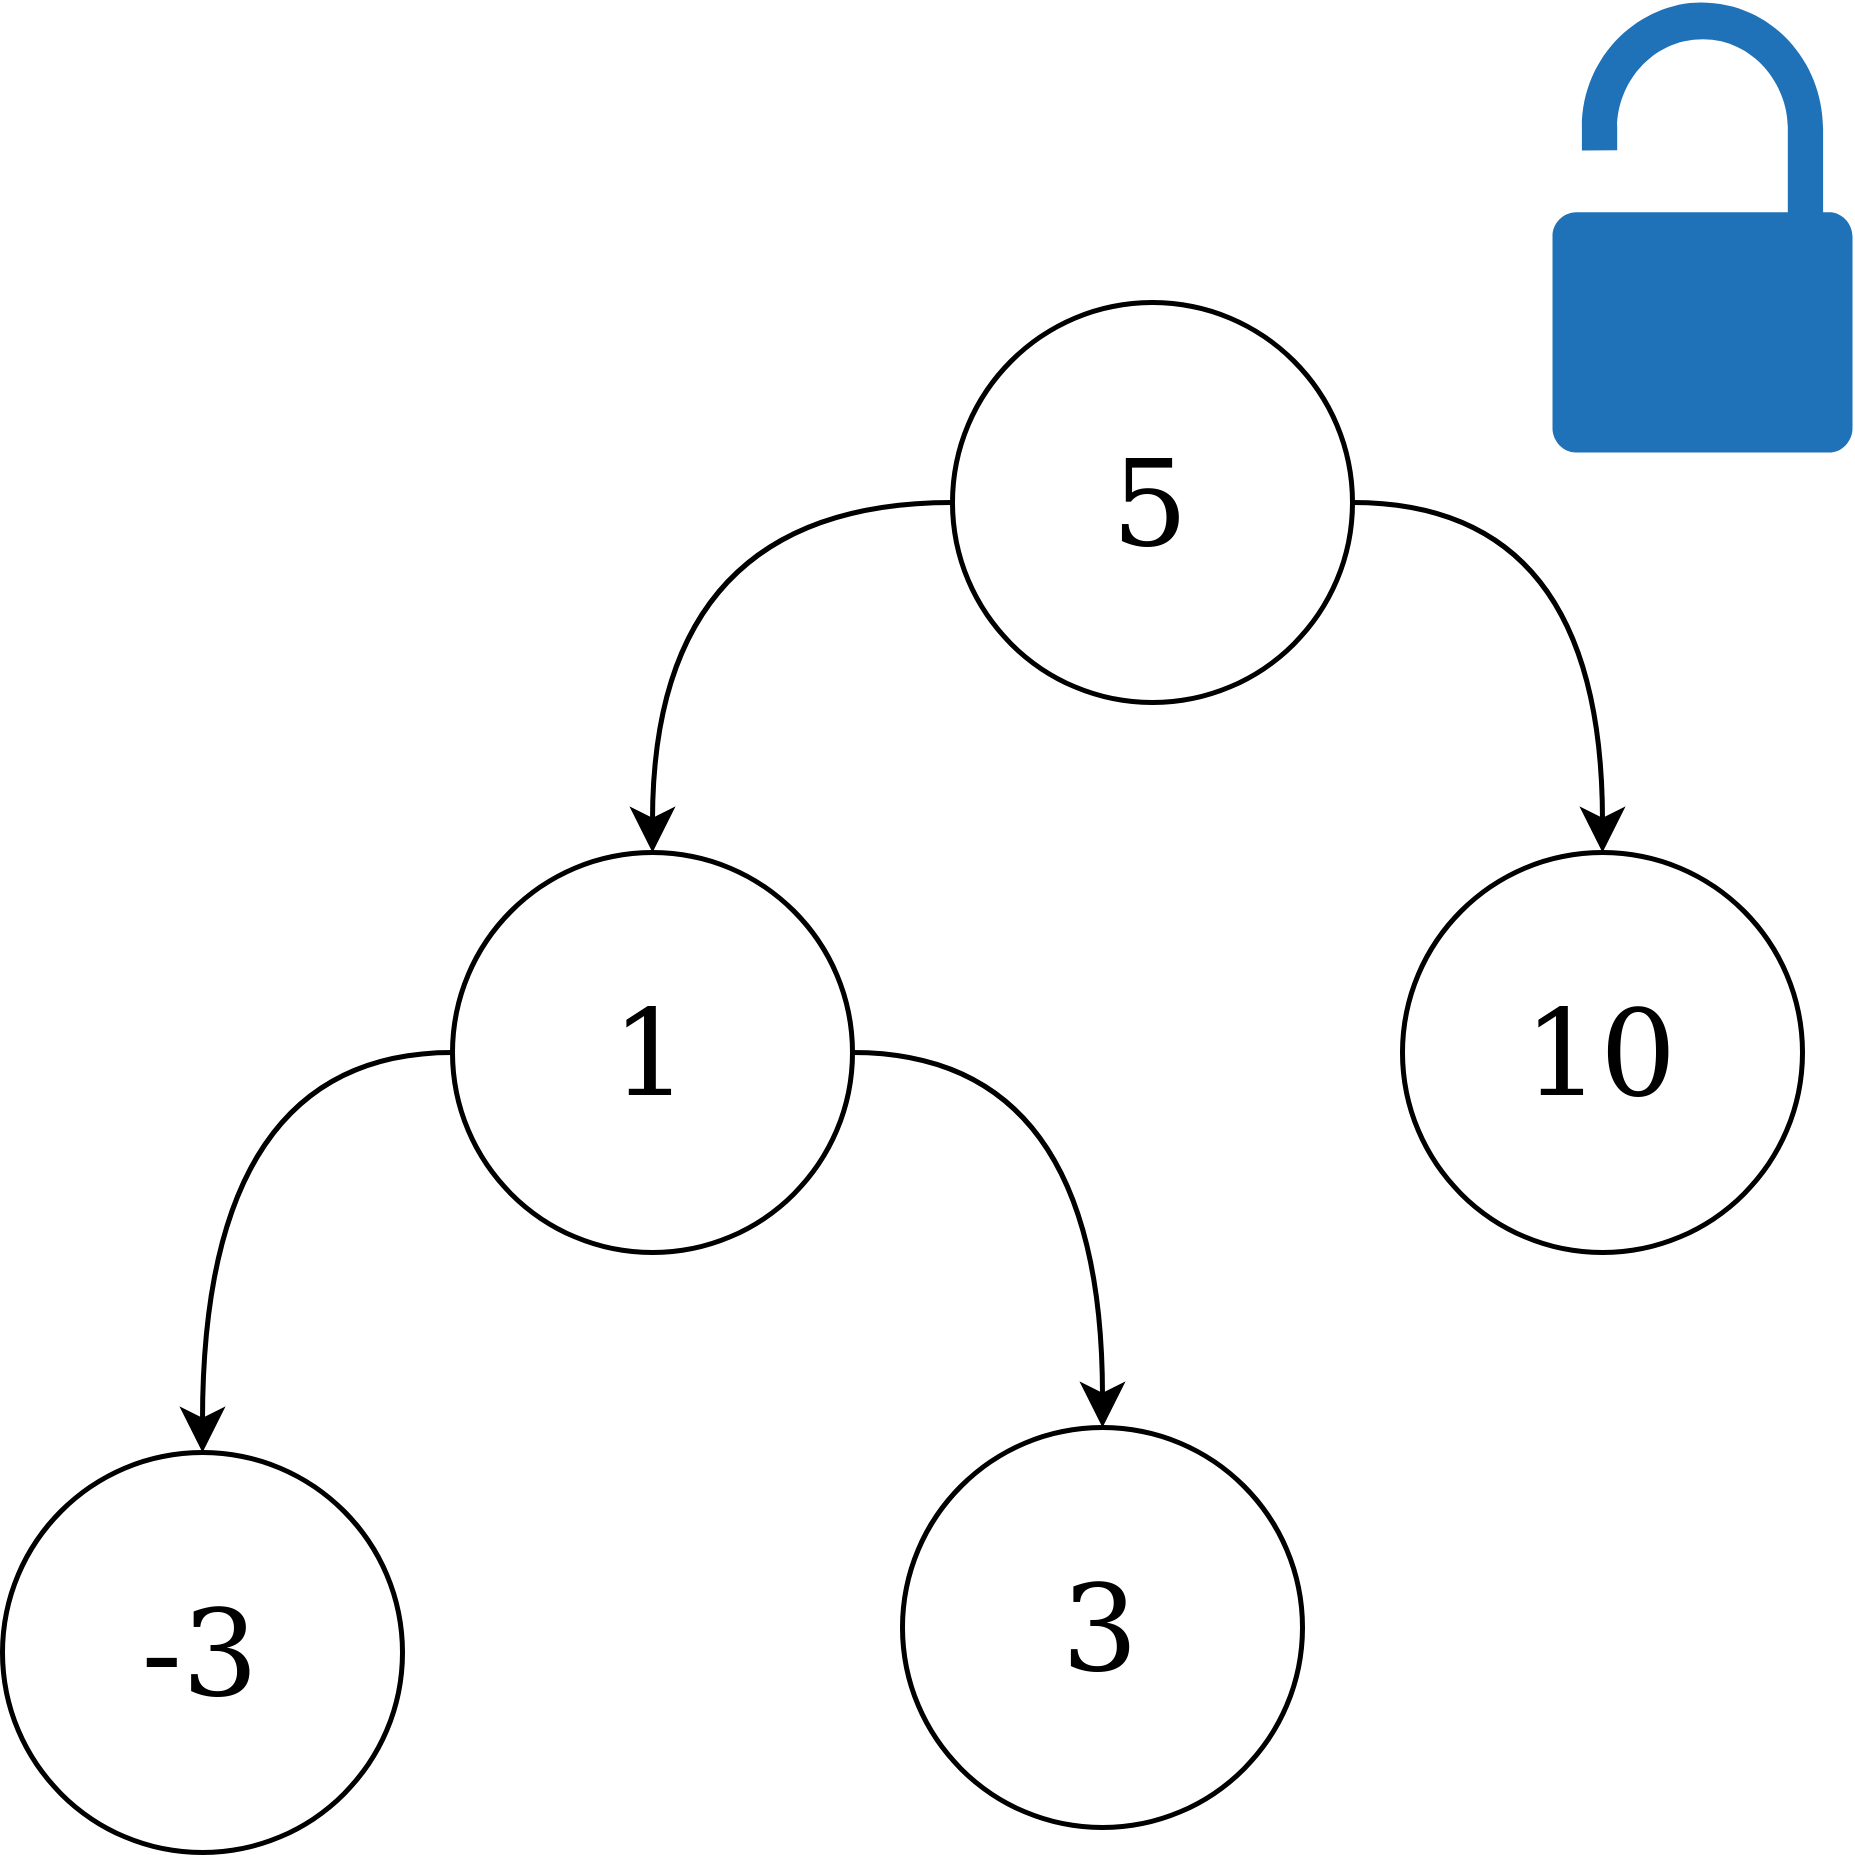
\includegraphics[width=0.5\linewidth]{pics/lock-solution.png}
\end{figure}


\subsection{Linear-time solutions}

A number of papers \cite{arbel2018harnessing, brown2012range} address the issue of executing lock-free range queries on concurrent trees. However, the aforementioned papers address only the \texttt{collect(min, max)} query, returning the list of keys, located within a range \texttt{[min; max]}. All other range queries are proposed to be implemented on top of the \texttt{collect} query. For example, the \texttt{count} query can be implemented as \texttt{count(min, max) = collect(min, max).length()}. 

This approach suffers from a major drawback: the \texttt{collect} query is executed in time, proportional to the length of the resulting list. Thus, for wide ranges, the query is executed in $O(N)$ time, since for wide ranges the result contains almost all the keys from the tree.

Thus, all range queries, implemented on top of the \texttt{collect} query, have $O(N)$ time complexity. However, this implementation is not asymptotically efficient: e,g, the \texttt{count} query can be executed in $O(\log N)$ time in a sequential environment instead of $O(N)$, as was shown in Section~\ref{sequential-algorithm}.

Therefore, despite being lock free, this method does not guarantee time efficiency, and thus cannot be used in environments, where low request latency is required.

\subsection{Solutions based on the Universal Construction}
\label{universal-constrcution-section}

These solutions are based on persistent data structures~\cite{persistent-data-structures}. Each modifying operation (e.g. \texttt{insert} or \texttt{remove}) creates a new version of the data structure without modifying the existing one. In order to reduce time and memory consumption, for a lot of persistent data structures the new version shares most of its nodes with the old version. 

For example, persistent trees can be implemented using \emph{path-copying} method~\cite{driscoll1989making}. This method merely copies each node on the path from the modified (e.g., inserted or removed) node to the root (Fig.~\ref{persistent-pic}), achieving $O(\log N)$ copied nodes in balances trees. 

\begin{figure}[H]
  \centering
  \caption{An example of a persistent tree with path-copying. \texttt{insert} operation creates new version of the data structure instead of modifying the existing one, the new version shares most of its nodes with the old version}
  \label{persistent-pic}
  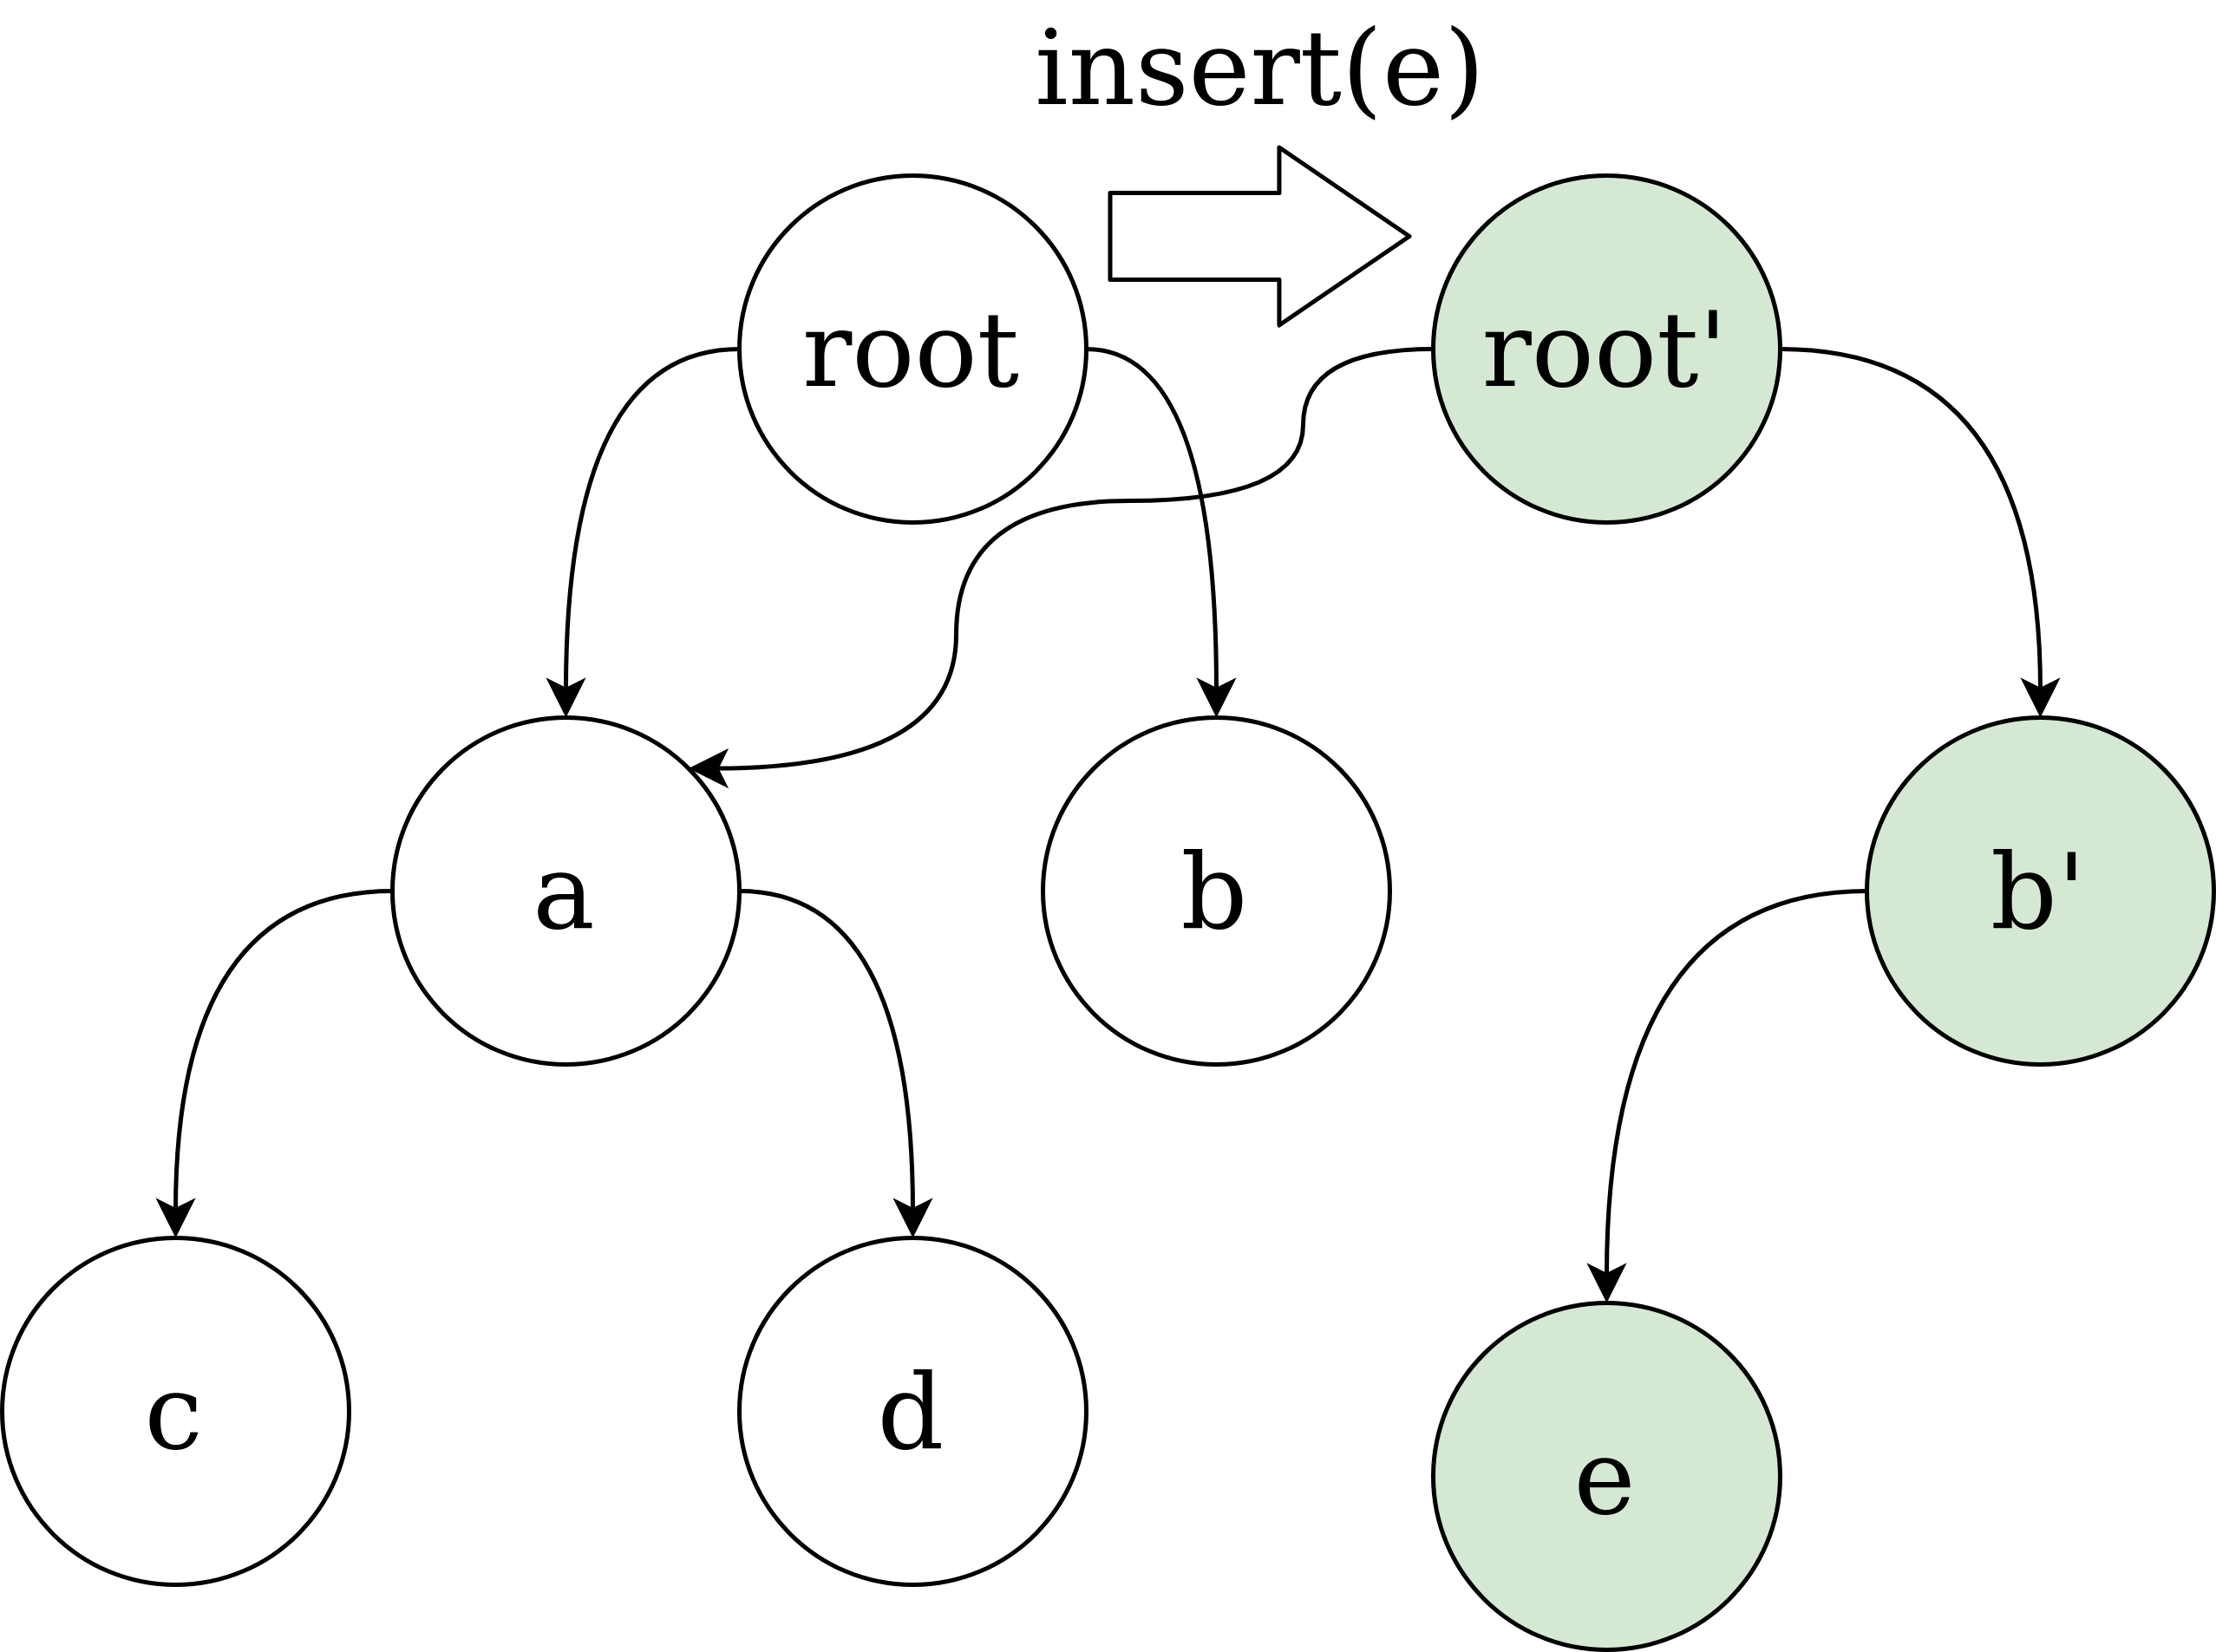
\includegraphics[width=0.7\linewidth]{pics/persistent-set.png}
\end{figure}

The basic idea of the Universal Construction, proposed first by Herlihy~\cite{herlihy1991wait}, is to store pointer to the root of the current version of the persistent data structure in the \texttt{read/CAS} register. Read-only queries (e.g. \texttt{contains} or \texttt{count}) on such data structures can be implemented very easily, no matter how complex are they: we just read the pointer to the latest version of the data structure and execute the query on it. Since the data structure is persistent, other processes cannot modify the fetched version, thus, it is completely safe to execute arbitrary read-only logic on the fetched version. For example, the \texttt{count} query can be implemented the following way (Listing~\ref{count-universal-construction-listing}):

\renewcommand{\lstlistingname}{Listing}
\begin{lstlisting}[caption={Universal Construction-based implementation of a \texttt{count} query},label={count-universal-construction-listing},escapeinside={(*}{*)}, captionpos=b]
fun count(Set, min, max):
    /*
    Other read-only operations (e.g. contains) can be 
    implemented the same way
    */
    cur_root := Set.Root_Pointer
    result := sequential_count(cur_root, min, max)
    return result
\end{lstlisting}

Update queries (e.g. \texttt{insert} or \texttt{remove}) are a bit more complex and have to go through the following steps:

\begin{nenum}
    \item Fetch \texttt{cur\_root}~--- the root of the current version of the data structure by reading the root pointer.
    
    \item Obtain \texttt{new\_root}~--- the root of the new version by executing the modification operation on the current version. Since the data is persistent, the current version is left unmodified.
    
    \item Use \texttt{CAS(\&Root\_Pointer, cur\_root, new\_root)} to atomically change the current version to the new version. If the \texttt{CAS} returns \texttt{true}, it means that we have successfully applied the modifying operation. Otherwise (if the \texttt{CAS} returns \texttt{false}), we conclude that some other process has already changed the version, performing its modification operation. In that case, we retry the whole operation from the very beginning, i.e., from step~(1).
\end{nenum}

\bigbreak

For example, \texttt{insert} operation can be implemented the following way (Listing~\ref{insert-universal-construction-listing}):

\renewcommand{\lstlistingname}{Listing}
\begin{lstlisting}[caption={Universal Construction-based implementation of the \texttt{insert} operation},label={insert-universal-construction-listing},escapeinside={(*}{*)}, captionpos=b]
fun insert(Set, key):
    /* 
    Other modification operations (e.g. remove) can be 
    implemented the same way 
    */
    while true:
        cur_root := Set.Root_Pointer
        new_root := persistent_insert(cur_root, key)
        if CAS(&Set.Root_Pointer, cur_root, new_root):
            return
        /* Otherwise, retry the whole operation from the very beginning */
\end{lstlisting}

This solution is lock-free, since each unsuccessful \texttt{CAS} indicates that some other process has successfully executed its operation (and changed the root pointer using \texttt{CAS}). The Universal Construction can even be implemented with a wait-free progress guarantee, as shown in~\cite{herlihy1991wait}.

However, despite being lock-free (or even wait-free) this solution suffers from a major drawback. Suppose we are executing multiple concurrent modification operations. Only one of them can be finished successfully, while others have to retry (Fig~\ref{universal-retry-pic}). To better understand the drawback, consider the following sequence of actions:

\begin{nenum}
    \item Process \texttt{P} tries to execute the operation \texttt{insert(2)}, fetches the current root pointer (\texttt{RP});
    
    \item Process \texttt{Q} tries to execute the operation \texttt{remove(5)}, fetches the current root pointer (\texttt{RP});
    
    \item Process \texttt{P} obtains the new version of the data structure (root pointer is $\texttt{RP}_{\texttt{P}}$), with key \texttt{2} inserted to the set;
    
    \item Process \texttt{Q} obtains the new version of the data structure (root pointer is $\texttt{RP}_{\texttt{Q}}$), with key \texttt{5} removed from the set;
    
    \item Process \texttt{P} successfully executes \texttt{CAS(\&Set.Root\_Pointer, RP, $\texttt{RP}_{\texttt{P}}$)};
    
    \item Process \texttt{Q} tries to execute \texttt{CAS(\&Set.Root\_Pointer, RP, $\texttt{RP}_{\texttt{Q}}$)} but fails to do so, because \texttt{Set.Root\_Pointer} now contains $\texttt{RP}_{\texttt{P}}$. Process \texttt{Q} has to retry the whole \texttt{remove(5)} operation from the beginning;
\end{nenum}

\begin{figure}[H]
  \centering
  \caption{Only one of multiple concurrent modifying operations can be executed successfully, the others have to retry}
  \label{universal-retry-pic}
  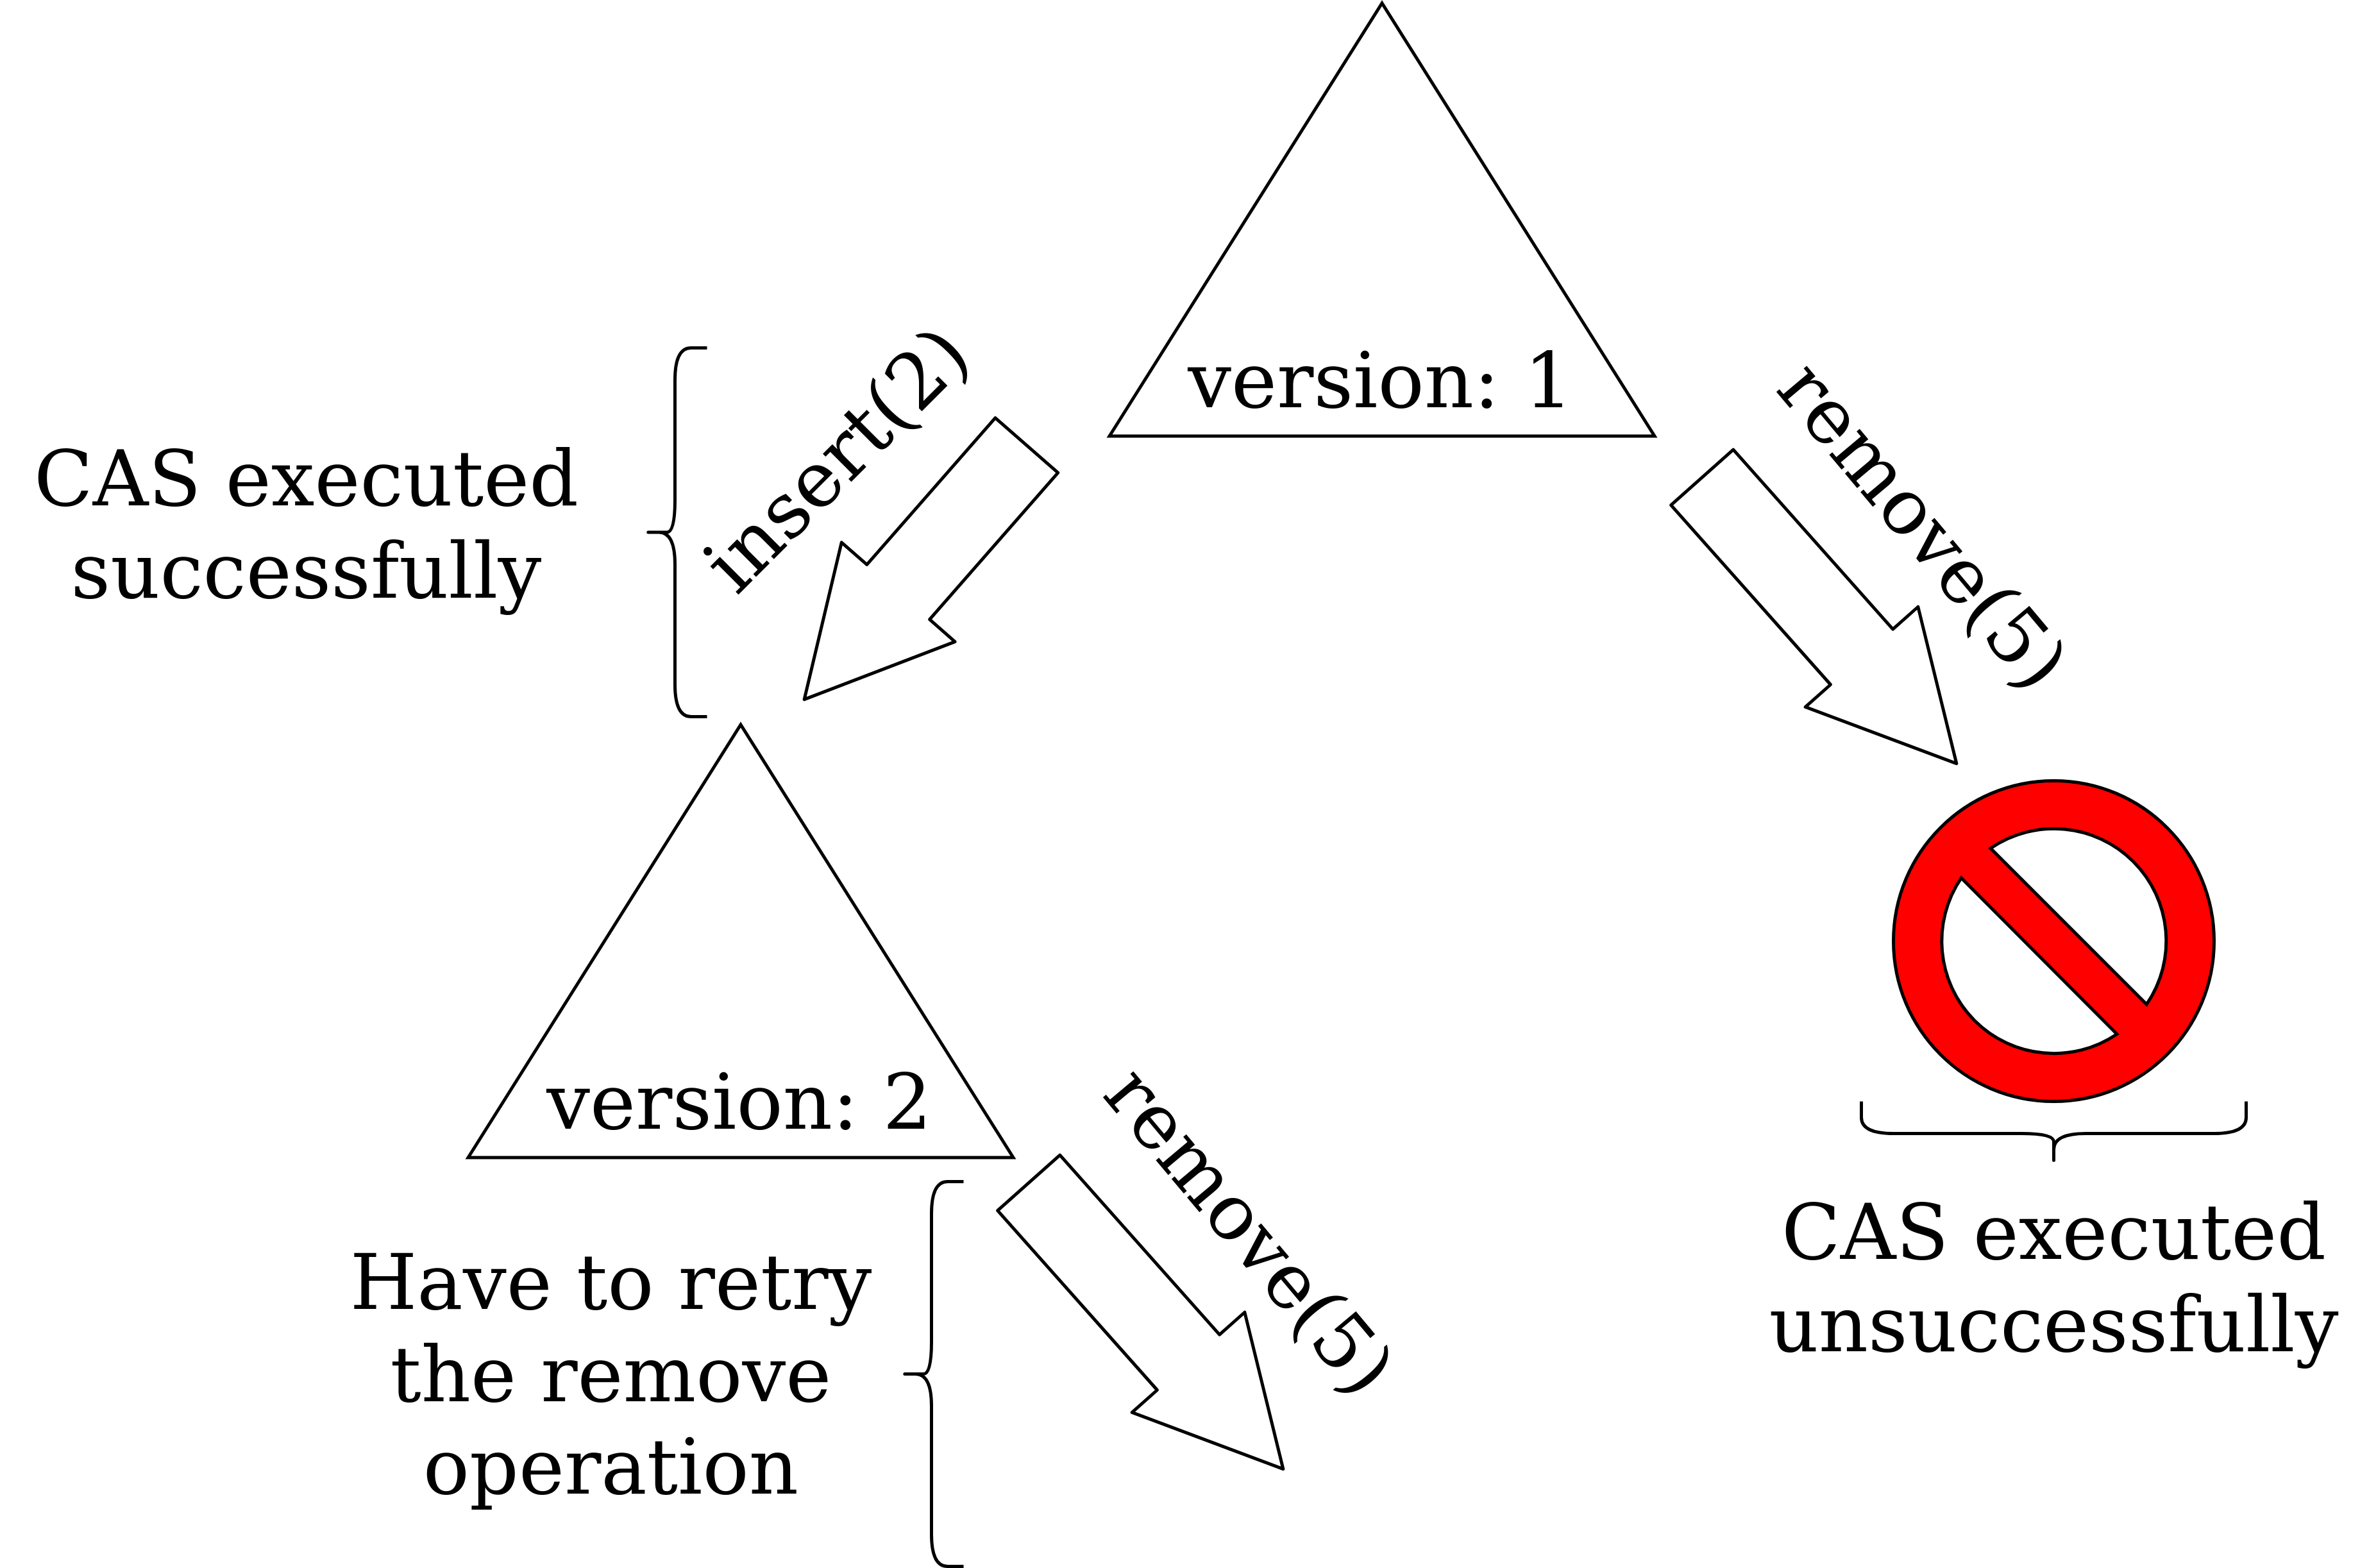
\includegraphics[width=\linewidth]{pics/universal-retry.png}
\end{figure}

Therefore, all modification operation are applied sequentially, one after another, making the data structure effectively sequential for modifications. This greatly reduces the throughput of the overall data structure and dramatically limits the scalability. Thus, Universal Construction-based data structures cannot be used in situations, when concurrent updates must be processed concurrently, instead of being processed one after another.

\subsection{Solutions, based on augmented persistent trees}

Sun, Ferizovic and Belloch~\cite{sun2018pam} addressed the problem of executing range queries on persistent trees. They proposed \emph{augmenting} each node of a persistent tree with an arbitrary value, that can be used to execute the range query faster (for example, the \texttt{count} query can be executed efficiently if each node of the tree is augmented with the size of its subtree).

However, the paper does not propose the method of executing concurrent operations on augmented data structures~--- only the method to execute a large batch of operations in parallel, e.g., an insertion of a batch of keys to the data structure (or a removal of a batch of keys from the data structure) using \emph{fork-join} parallelism to speed up the execution.

Therefore, in some cases this method simply cannot be used~--- for example, when updates do not come in large batches. In cases, when there is a large number of concurrent single-value updates instead of a small number of batch updates, following sequentially, one after another, we cannot use augmented persistent trees as-is.

We can use various combining techniques~\cite{hendler2010flat,aksenov2017parallel} to form large batches of updates from individual concurrent updates (Fig.~\ref{transaction-batching-pic}). However, combining techniques increase individual operation latency and thus they are not acceptable in settings, where low operation latency is required.

\begin{figure}[H]
  \centering
  \caption{Forming batches of updates from individual concurrent updates}
  \label{transaction-batching-pic}
  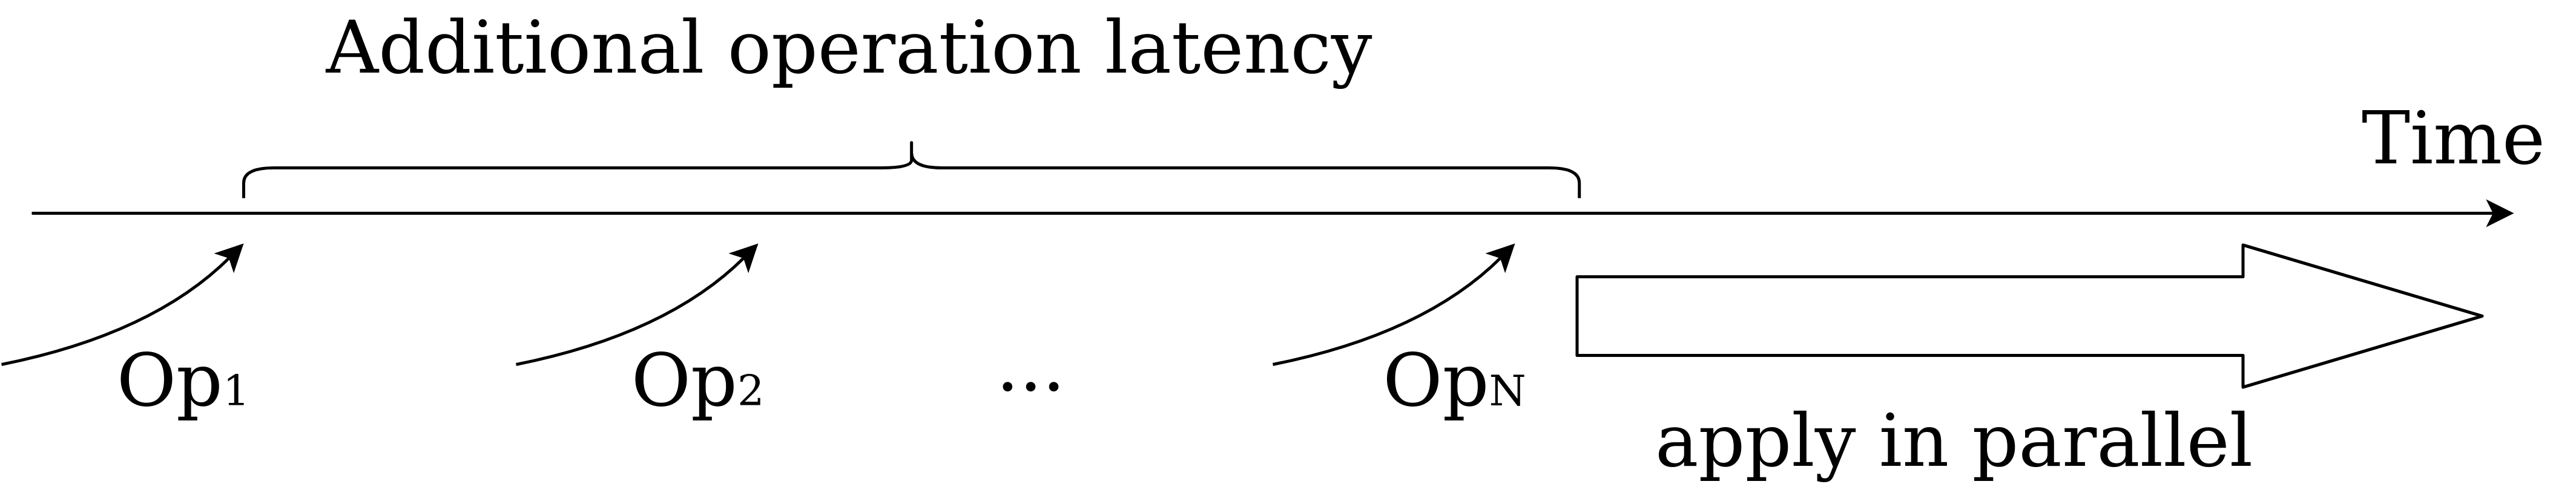
\includegraphics[width=\linewidth]{pics/transaction-batching.png}
\end{figure}

\finishrelatedwork

\chapterconclusion

In this chapter, we have performed a review of the subject area. We have reviewed the notion of a tree, the notion of range queries, along with the sequential time-efficient algorithm for execution of the \texttt{count} range query. We glanced over some examples of how efficient range queries can be used in modern databases. Also, we reminded the basics of concurrent computing: the notion of concurrency, along with concurrent correctness criteria, and concurrent progress guarantees. Finally, we studied modern solutions to the problem of executing range queries on concurrent trees and made sure, that all actual solutions suffer from various drawbacks, which we ought to overcome in this work.

\chapter{General description of the algorithm}
\label{algorithm-general-chapter}

\section{Concurrent solution: the main invariant}
\label{main-invariant-chapter}

The main problem with the sequential algorithm, described in Section~\ref{sequential-algorithm}, is that in a concurrent environment it will be incorrect. Indeed, each modifying operation (e.g. \texttt{insert} or \texttt{remove}) should modify not only the tree structure, but the augmentation values (e.g., subtree sizes) too. Thus, augmentation values may become inconsistent with the tree structure (Fig.\ref{inconsistency-pic}). In that case, the process executing a \texttt{count} query is not able to execute it correctly, given such an inconsistent view of the tree.

\begin{figure}[H]
  \centering
  \caption{Tree structure is inconsistent with the augmentation value: while both leaves have already been removed from the tree the subtree size is still two.}
  \label{inconsistency-pic}
  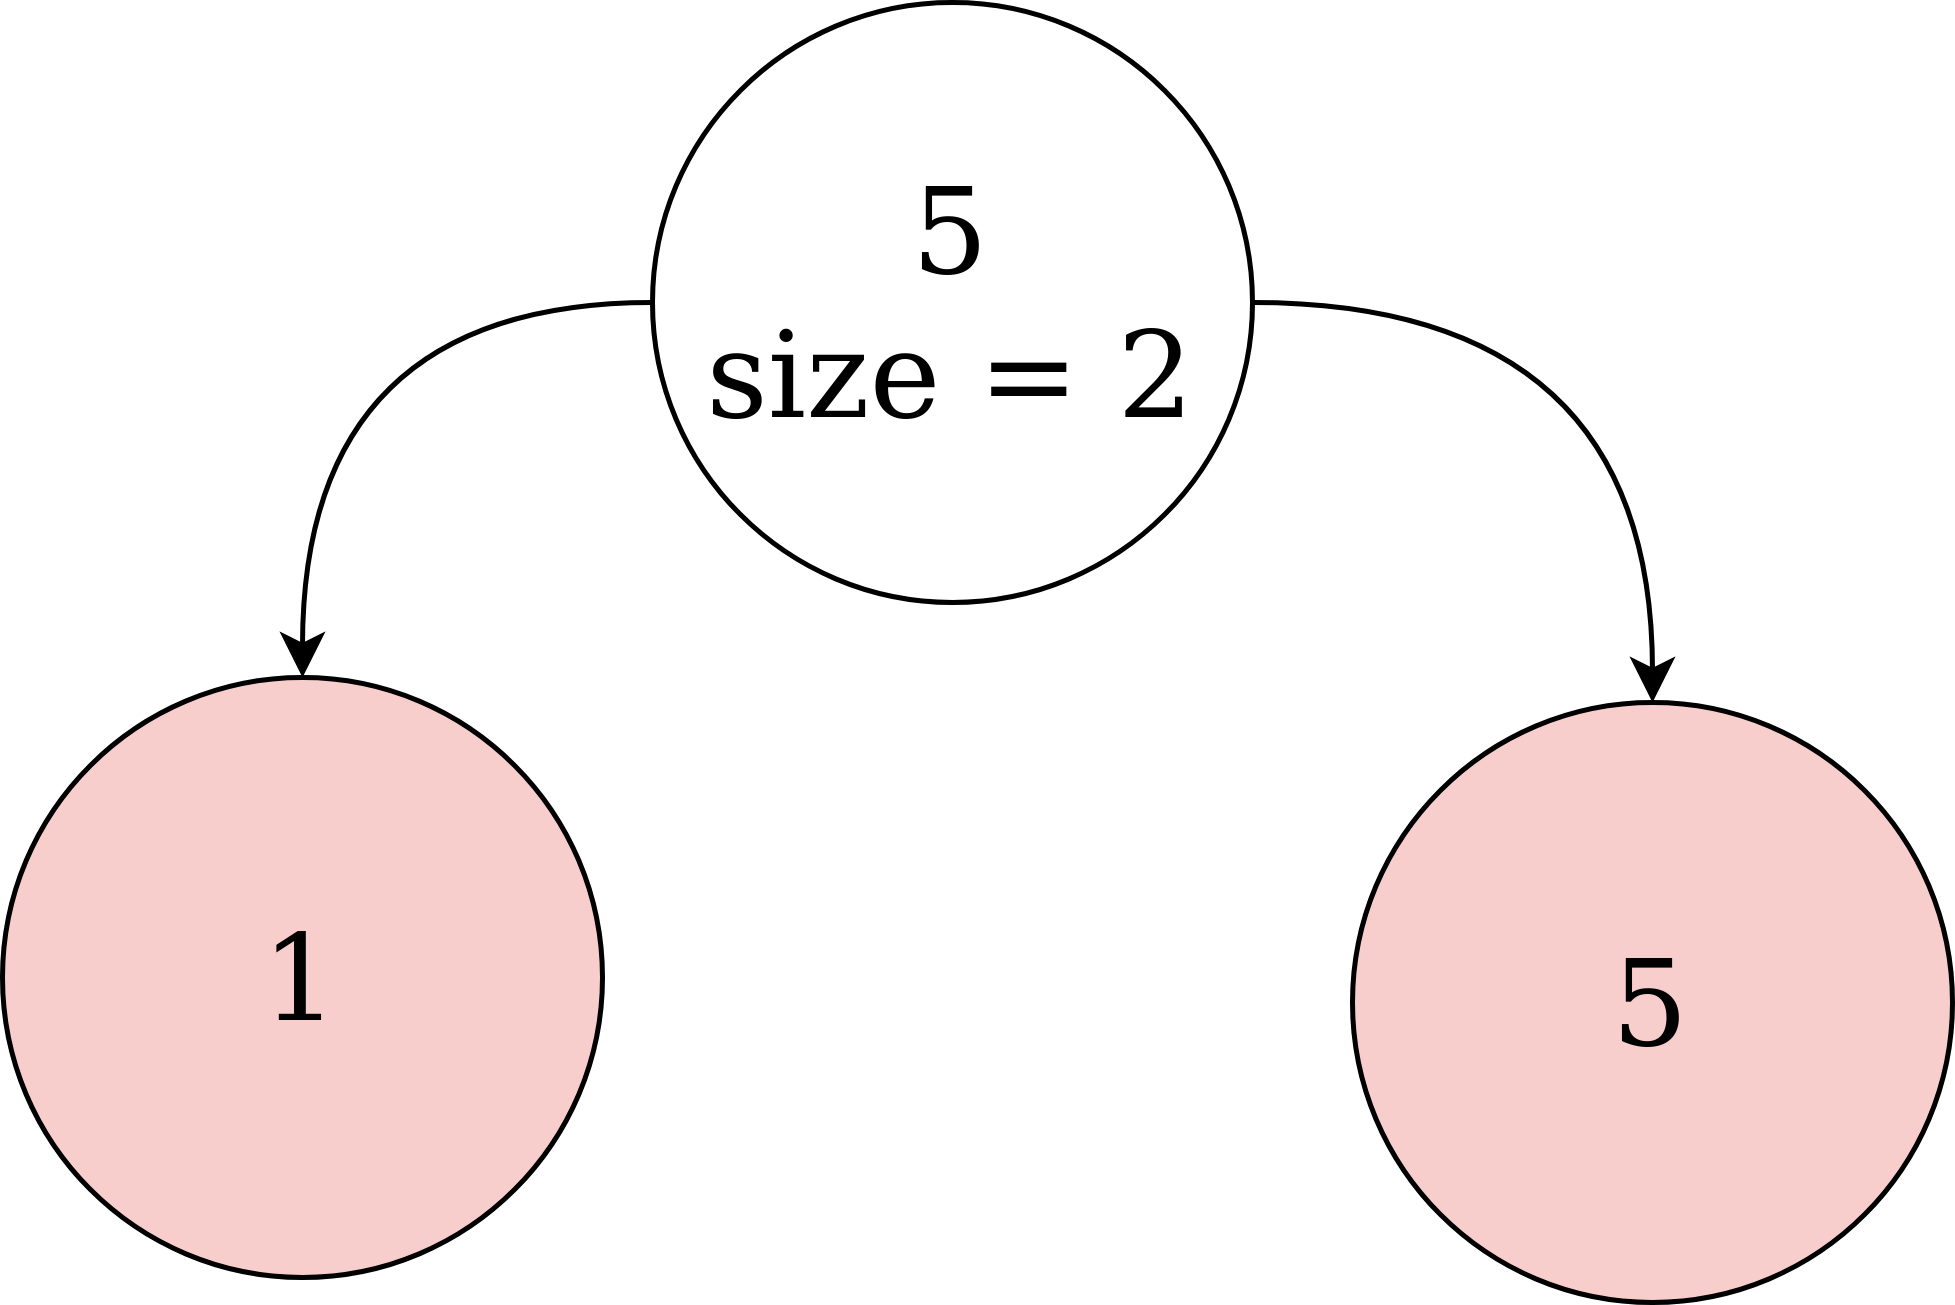
\includegraphics[width=0.5\linewidth]{pics/inconsistency.png}
\end{figure}

Therefore, the main purpose of our concurrent solution is to get rid of such situations by ensuring that all operations are executed in a particular order. We will enforce a particular execution order by maintaining operation queue in each node.

Consider an arbitrary node \texttt{v} and its subtree \texttt{vs}. At \texttt{v} we maintain \emph{operations queue}, that contains descriptors of operations to be applied to  \texttt{vs} (Fig.~\ref{main-invariant-pic}). These operations can, for example, insert a key to \texttt{vs} or remove a key from \texttt{vs}. We maintain the following invariant: operations should be applied to \texttt{vs} in the order, their descriptors were added to \texttt{v} queue.

\begin{figure}[H]
  \centering
  \caption{Node \texttt{v} contains operations queue with descriptors of three operations: $\texttt{Op}_{\texttt{1}}$, $\texttt{Op}_{\texttt{2}}$ and $\texttt{Op}_{\texttt{3}}$. These three operations should be applied to \texttt{vs} in the order of descriptors in the queue: first $\texttt{Op}_{\texttt{1}}$, then $\texttt{Op}_{\texttt{2}}$, and, finally, $\texttt{Op}_{\texttt{3}}$}
  \label{main-invariant-pic}
  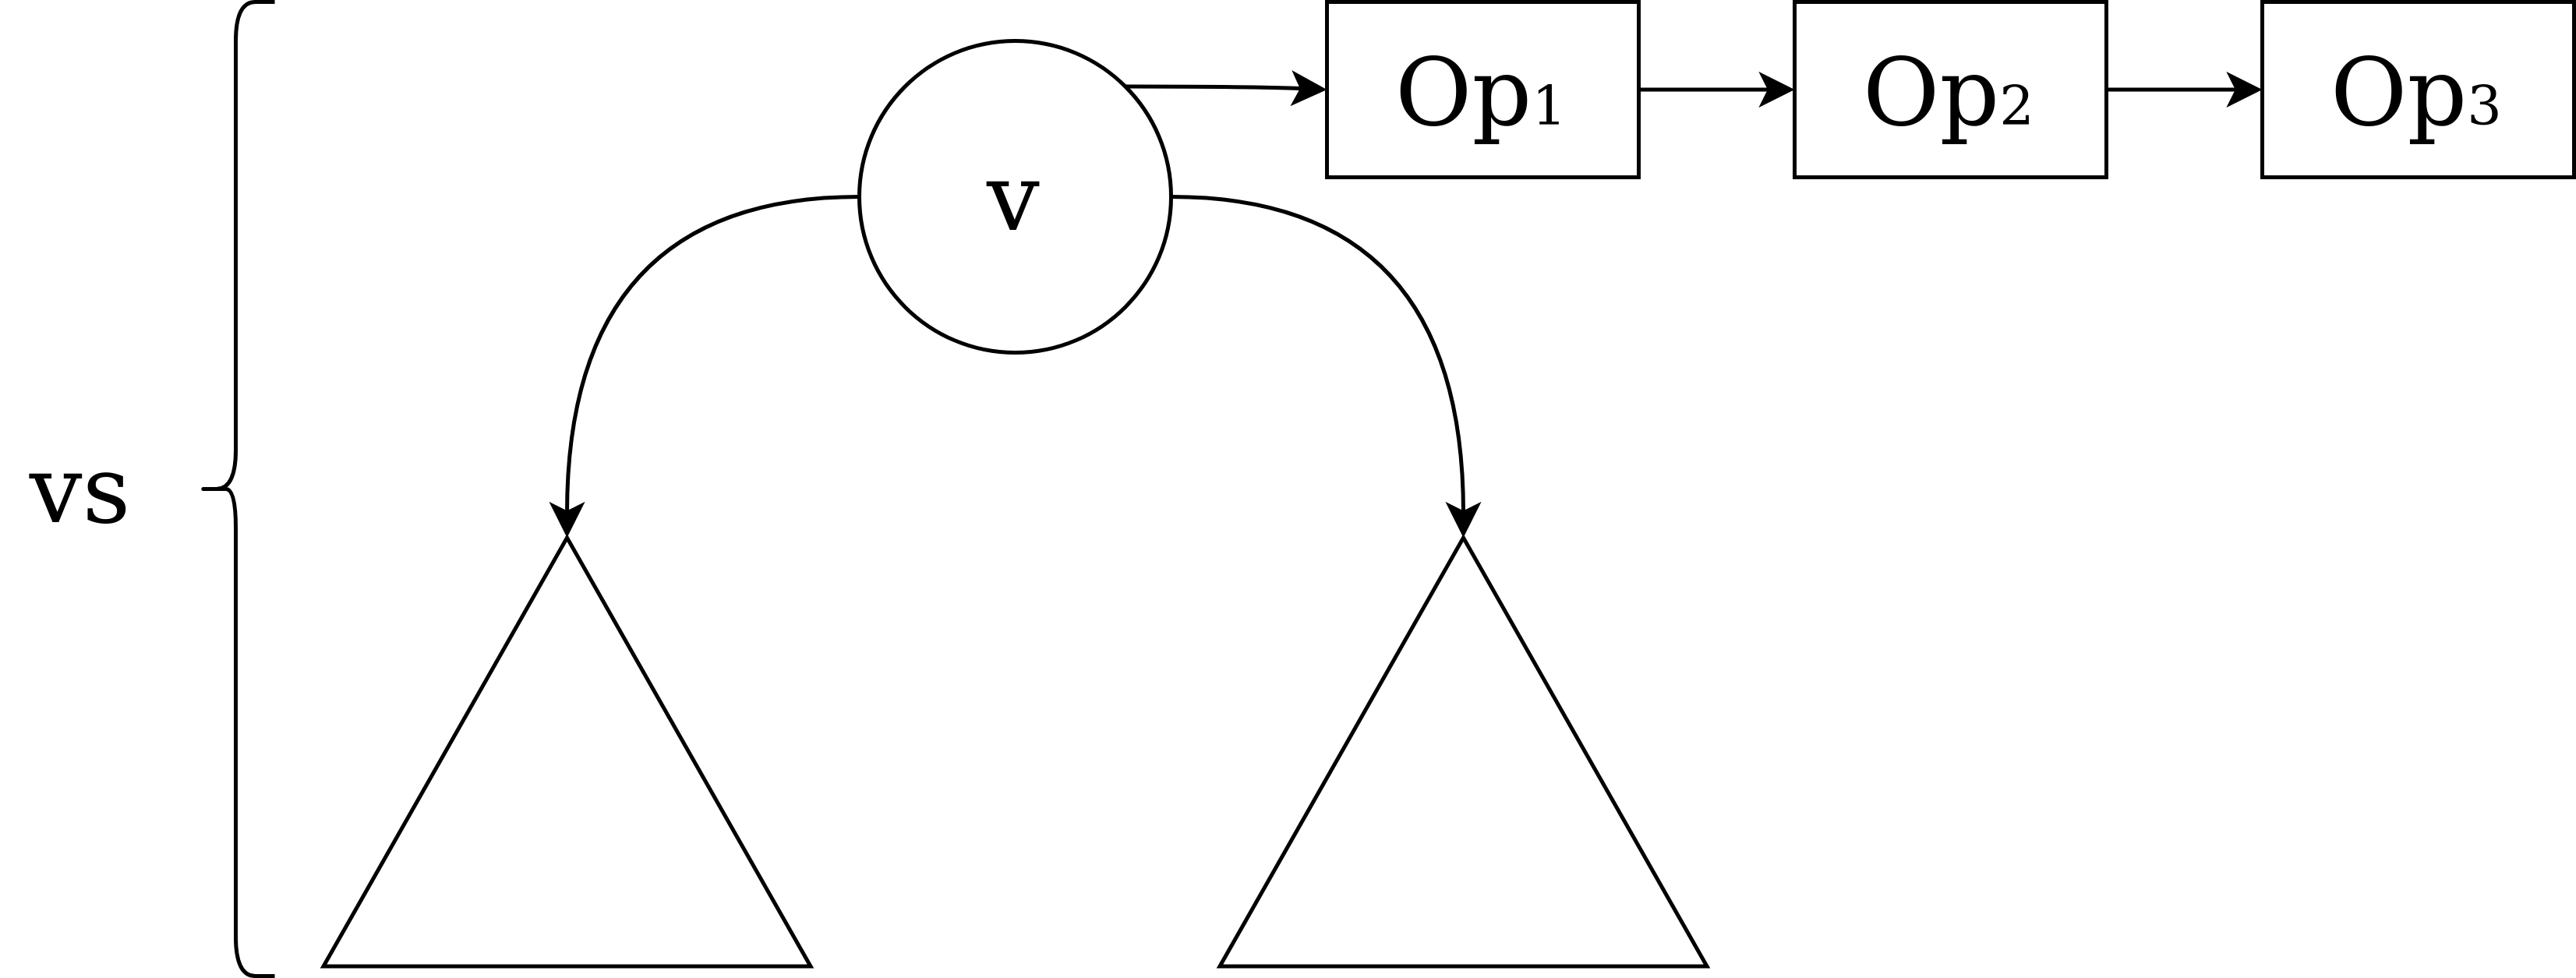
\includegraphics[width=\linewidth]{pics/main-invariant.png}
\end{figure}

Note, that the aforementioned invariant can be applied to the root node too: indeed, since the whole tree is just the root's subtree, operations should be applied to the tree in the order their descriptors were added to the root operation queue. Thus, the order, in which operation descriptors are added to the root operation queue, is exactly the \emph{linearization order}, in which the operations should seem to be applied to the tree.

Thus, we may use the operation queue at the root node to allocate timestamps for operations. Timestamp allocation mechanism should provide the following guarantee: if descriptor of operation \texttt{A} was added to the root queue before descriptor of operation \texttt{B}, then \texttt{timestamp(A) $<$ timestamp(B)} should hold. In Section~\ref{push-acquire-timestamp-section}, we will show how such timestamp allocation mechanism can be implemented. Since, the order, in which operation descriptors are added to the root queue, equals to the linearization order, operations should linearize in the order, determined by their timestamps. For example, operation \texttt{A} should precede operation \texttt{B} in the sequential execution $\mathbb{L}$ from the linearizability definition (that is described in Section~\ref{correctness-criteria-section}). Therefore, the following three orders will be the same:

\begin{itemize}
    \item The linearization order $\mathbb{L}$.
    
    \item The \emph{timestamp order}: operation \texttt{A} precedes operation \texttt{B} in the timestamp order if \texttt{timestamp(A) < timestamp(B)}.
    
    \item The order, in which operation descriptors were added to the root queue.
\end{itemize}

\bigbreak

As described in Section~\ref{operation-execution-chapter}, system processes want to examine timestamps of different operations during the operation execution. To allow them do so, we include the operation timestamp in the operation descriptor and store it in the \texttt{descriptor.Timestamp} field.

\section{Operation execution: overview}
\label{operation-execution-chapter}

At first, we start with unbalanced trees. One possible balancing strategy via subtree rebuilding is discussed in Section~\ref{balancing-section}, while studying other concurrent balancing strategies we leave for the future work.

The execution of an operation \texttt{Op} by a process \texttt{P} (we call process \texttt{P} the \emph{initiator} process) begins with inserting the descriptor of \texttt{Op} into the root queue and obtaining the operation timestamp. In Section~\ref{push-acquire-timestamp-section}, we describe, how the root queue with lock-free timestamp allocation may be implemented.

After that, the initiator process starts traversing the tree downwards, from the root to the appropriate lower node, i.e. to the node, at which the operation (e.g., insertion of a new data item, or removal/modification of an existing one) should be performed (Fig.~\ref{traversal-to-node-pic}).

\begin{figure}[H]
  \centering
  \caption{Execution of operation \texttt{insert(31)} in an external binary search tree consists of traversing the tree from the root downwards to the leaf, where key \texttt{31} should be inserted.}
  \label{traversal-to-node-pic}
  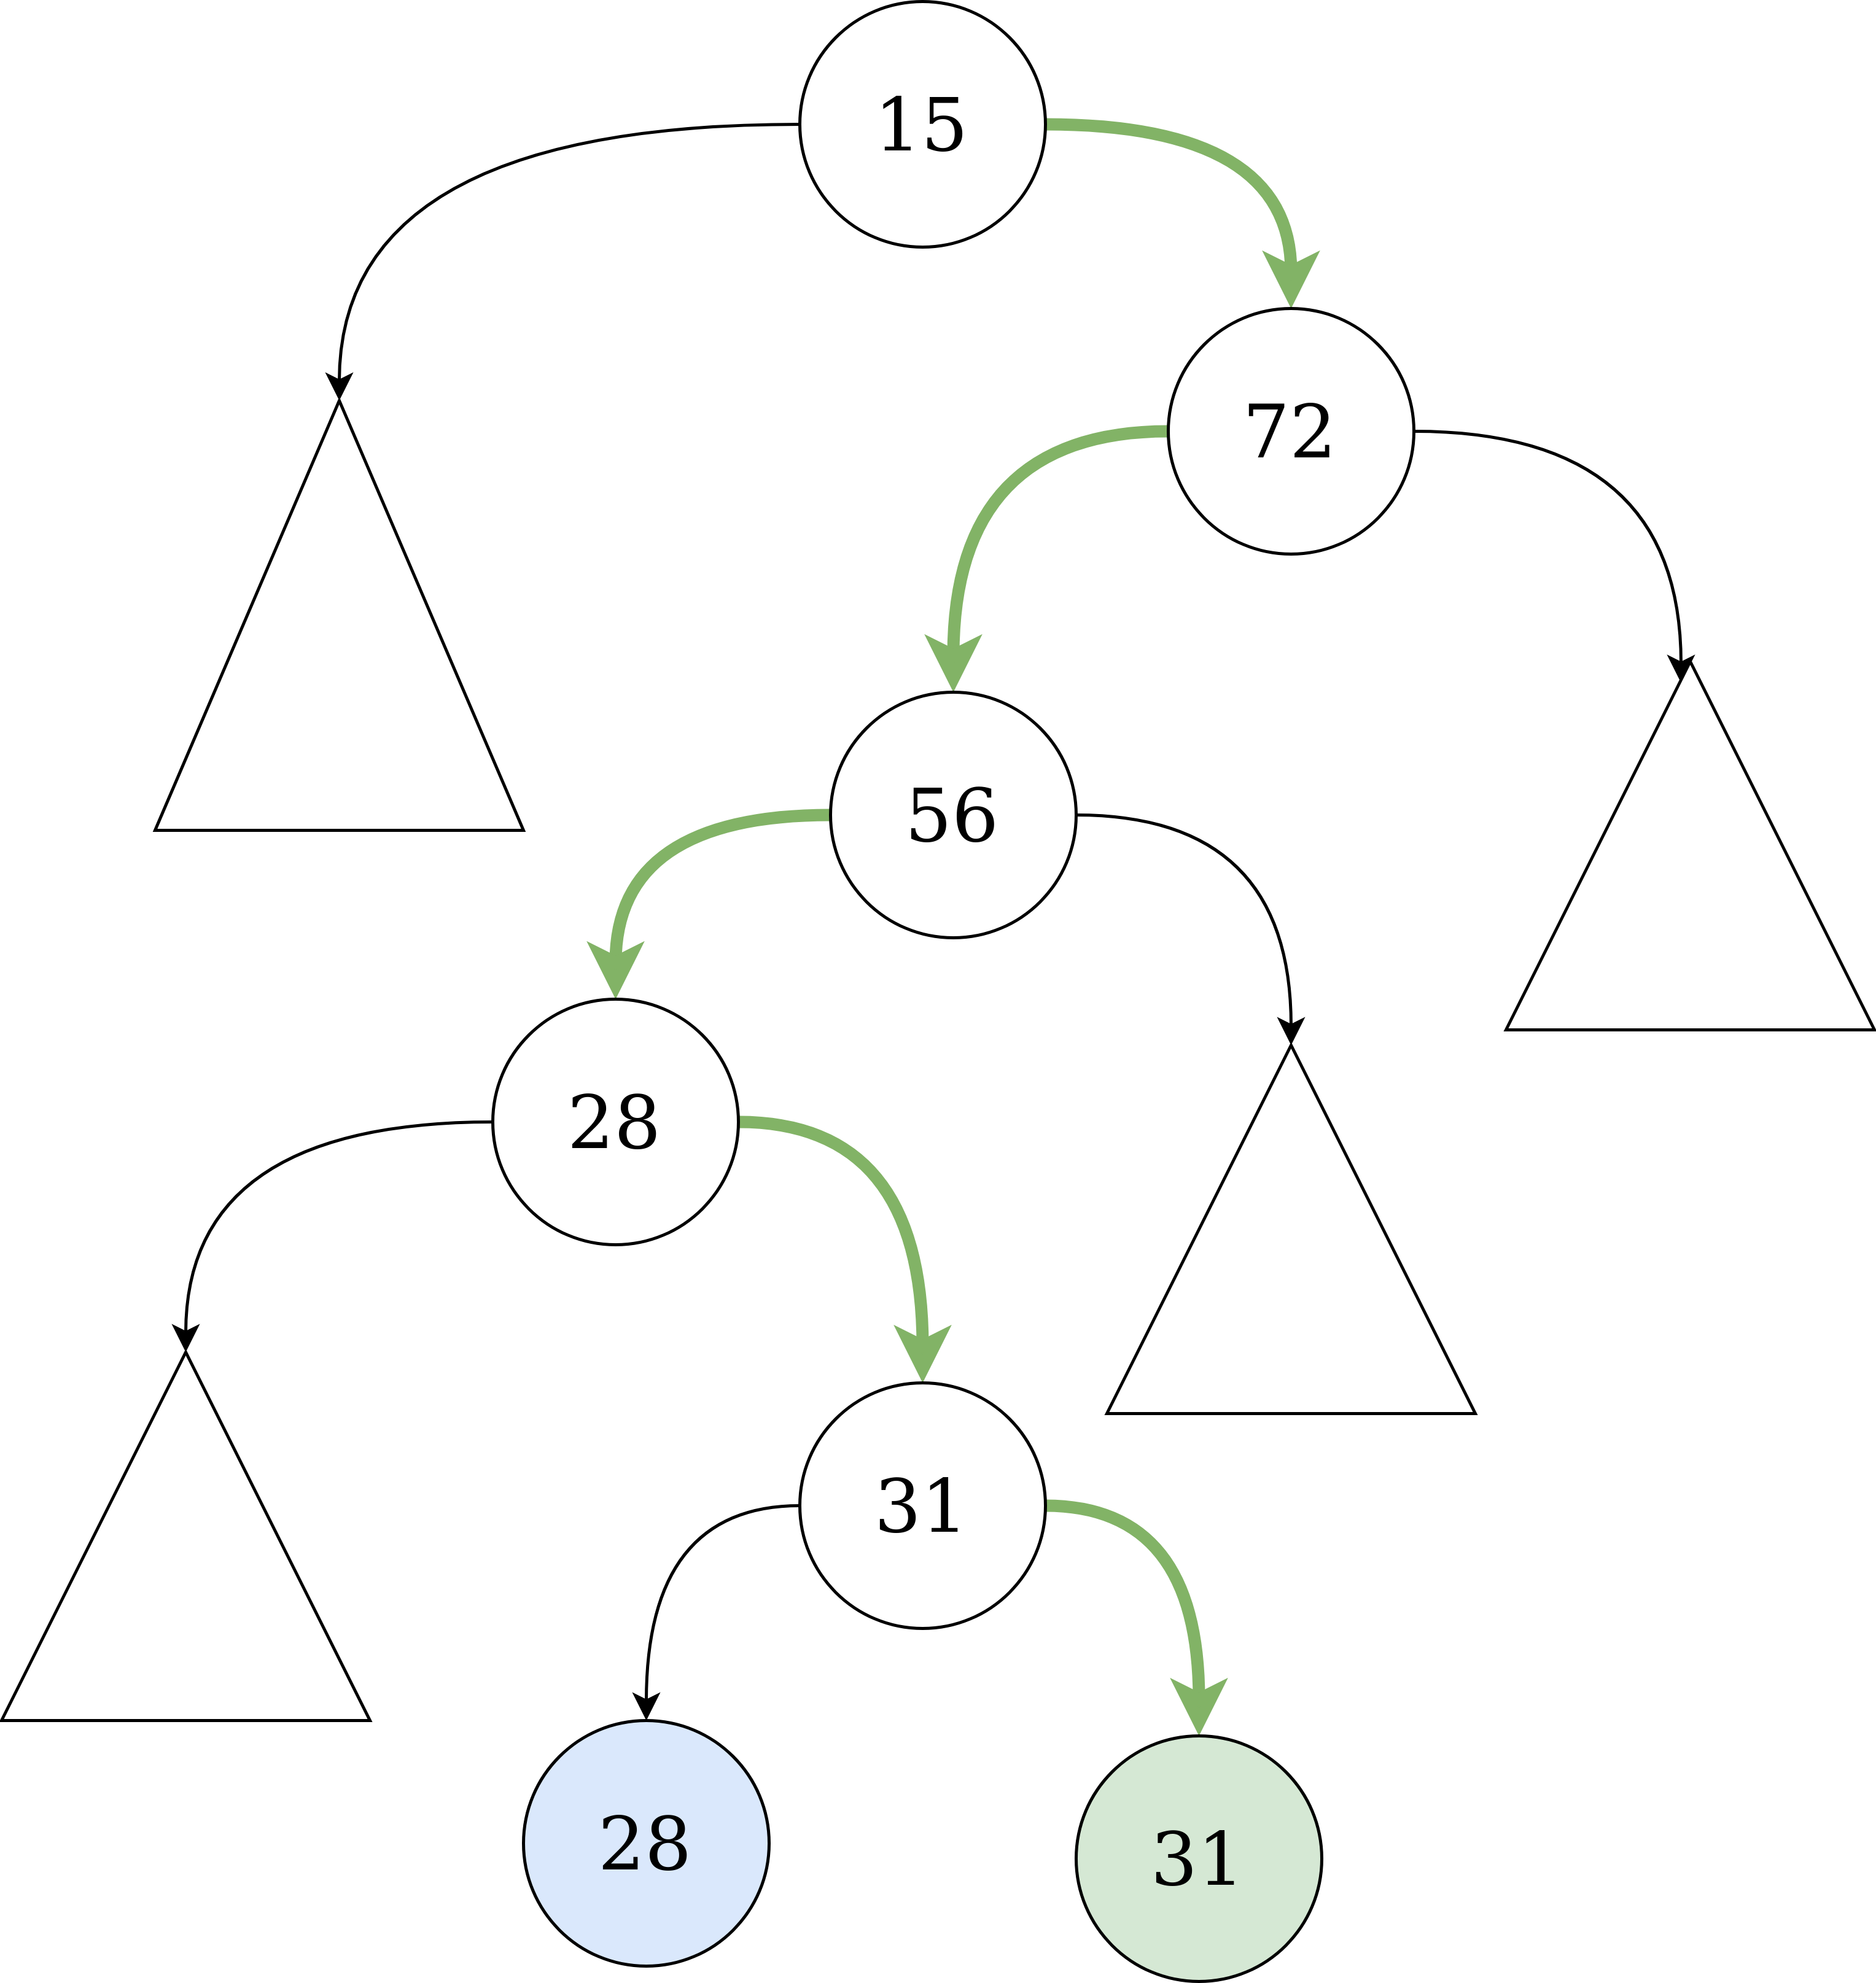
\includegraphics[width=\linewidth]{pics/traversal-to-node.png}
\end{figure}

\begin{definition}
In each visited node \texttt{v} some actions should be performed, in accordance with the meaning of the operation \texttt{Op} being executed. For example, size of \texttt{v} subtree or pointers to \texttt{v} children should be changed during \texttt{insert} or \texttt{remove} operation. We call the process of performing these actions \emph{execution of operation \texttt{Op} in node \texttt{v}}.
\end{definition}

As stated in Section~\ref{main-invariant-chapter}, operations should be applied to \texttt{v} subtree in the order operation descriptors are inserted to \texttt{v} queue. Thus, if the descriptor of \texttt{Op} is not located at the head of \texttt{v} queue the initiator process \texttt{P} will have to wait for the ability to begin executing \texttt{Op} in node \texttt{v} (Fig.~\ref{operation-execution-waiting-pic}). The execution of \texttt{Op} in node \texttt{v} cannot begin until execution of all preceding operations in node \texttt{v} is finished.

\begin{figure}[H]
  \centering
  \caption{Process \texttt{P} has to wait for ability to begin executing \texttt{Op} in node \texttt{v}, since only the operation $\texttt{D}_{\texttt{0}}$, corresponding to the descriptor at the head of \texttt{v} queue, can be executed in \texttt{v}.}
  \label{operation-execution-waiting-pic}
  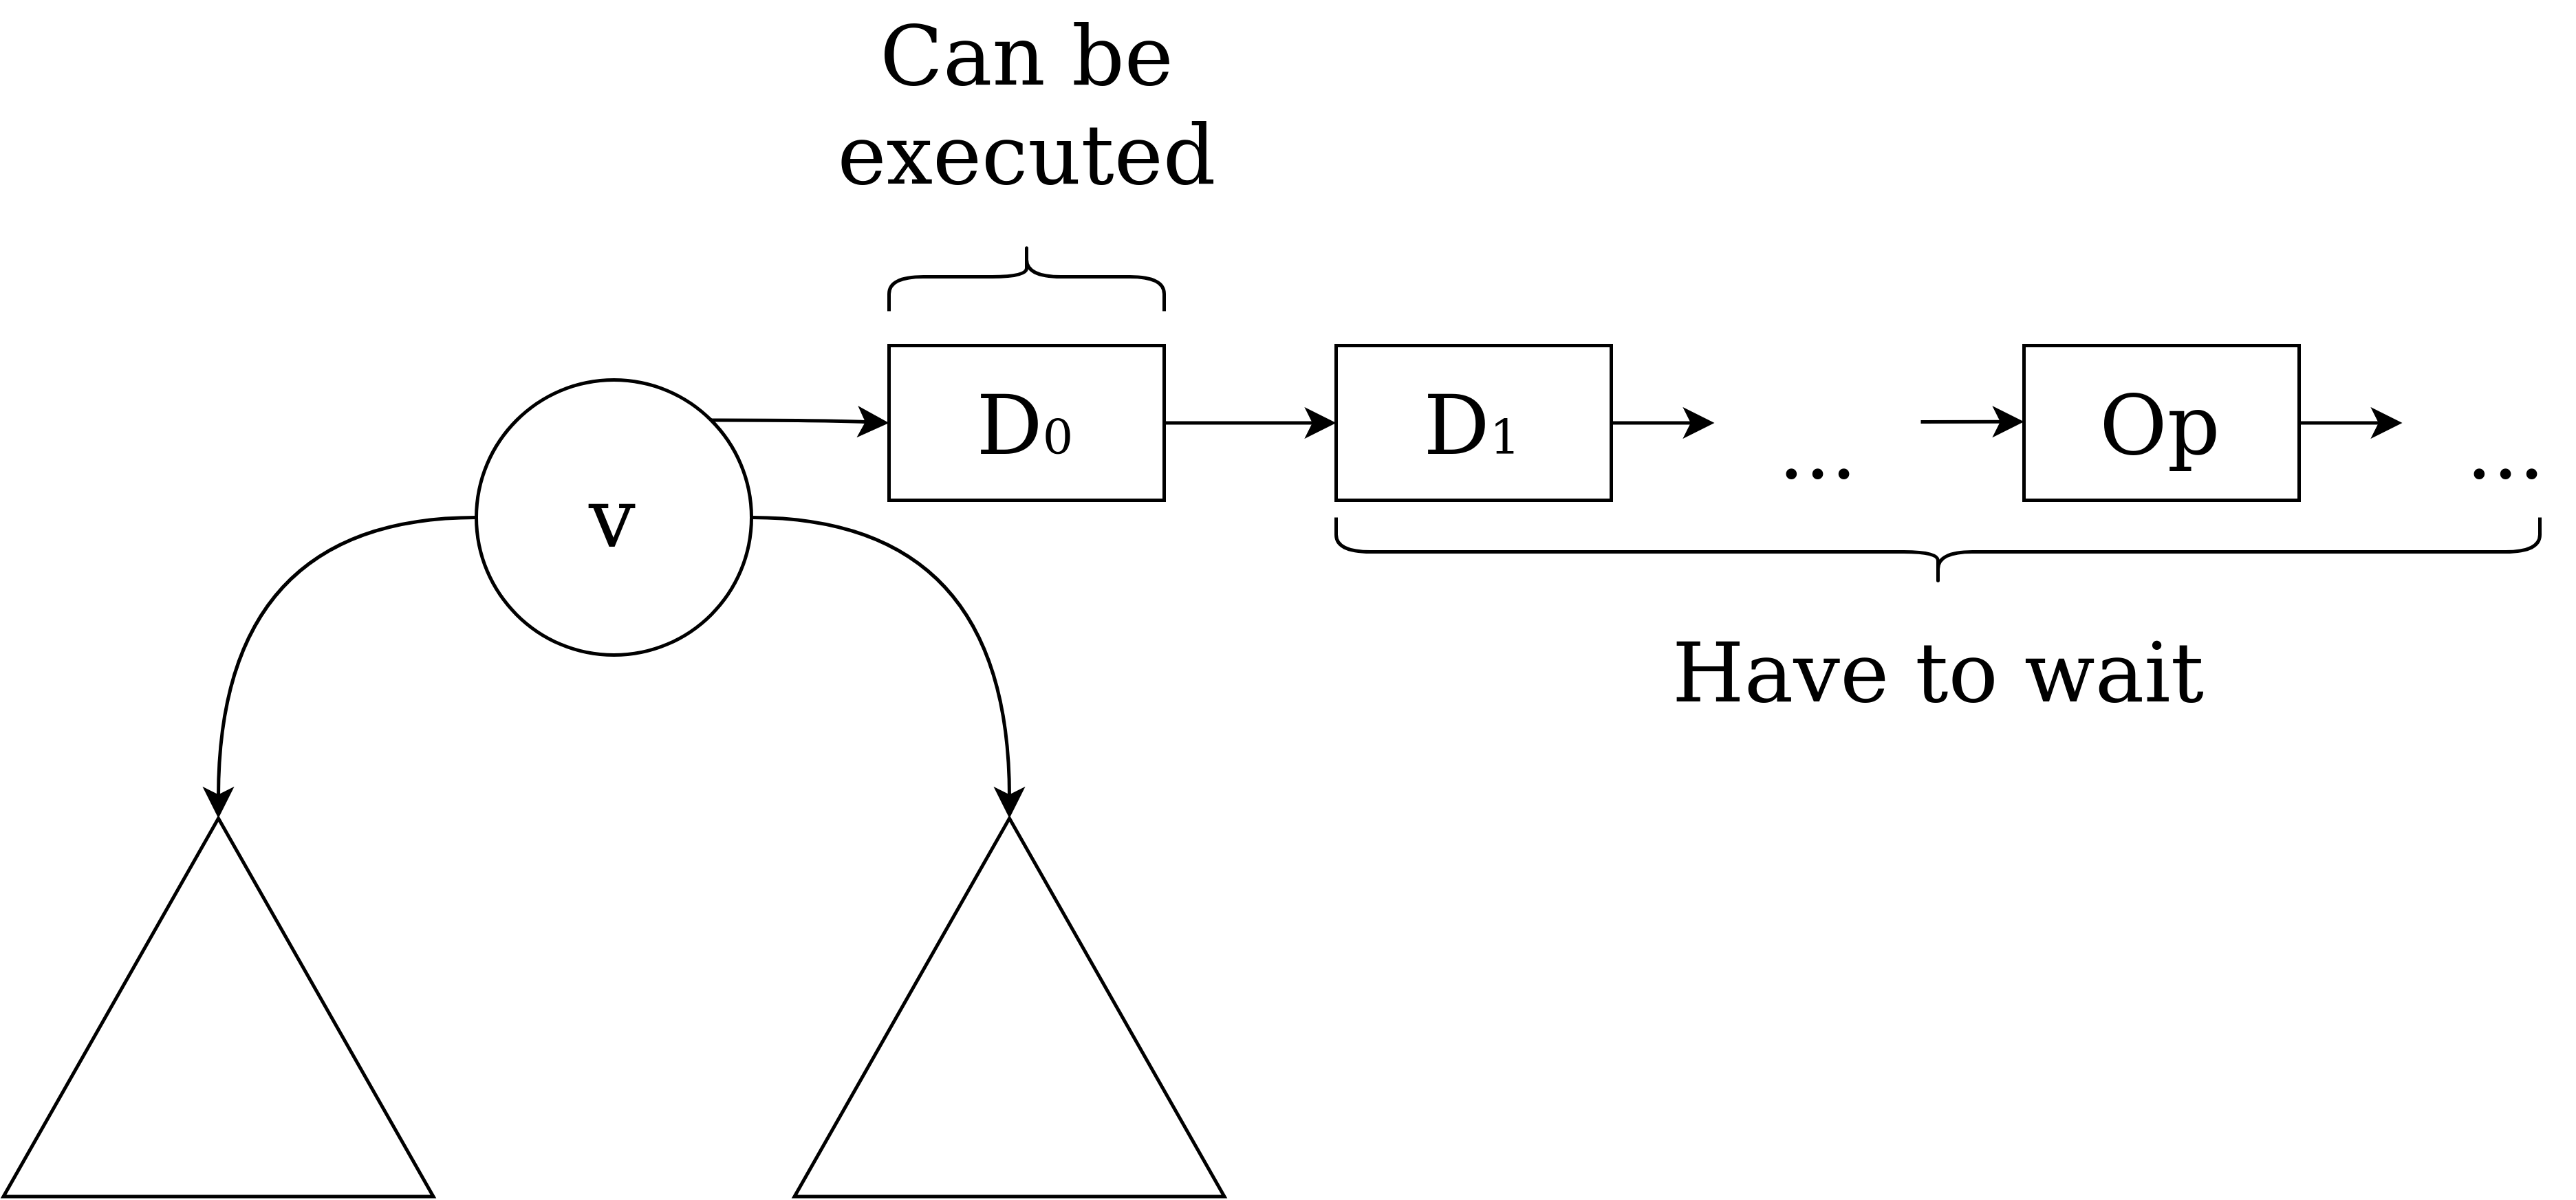
\includegraphics[width=\linewidth]{pics/operation-execution-waiting.png}
\end{figure}

The algorithms seems to be blocking, but that is where the \emph{helping} mechanism comes to the rescue. Instead of simply waiting for the \texttt{Op} descriptor to move to the head of the queue, \texttt{P} helps executing in node \texttt{v} the operation from the head of \texttt{v} queue~--- $\texttt{D}_{\texttt{0}}$ in the example above. Thus, even if the initiator process of $\texttt{D}_{\texttt{0}}$ is suspended, the system still achieves progress. 

As discussed later, while helping to execute operations $\texttt{D}_{\texttt{0}}, \texttt{D}_{\texttt{1}}, \ldots$ in node \texttt{v} the process \texttt{P} removes their descriptors from the head of \texttt{v} queue and inserts them to the appropriate child queues. Thus, while helping other processes execute their operations in \texttt{v}, \texttt{P} moves \texttt{Op} descriptor closer to the head of \texttt{v} queue. Once \texttt{P} helps all preceding operations to finish their execution in node \texttt{v}, it can finally begin executing \texttt{Op} in \texttt{v}.

The process of executing an operation \texttt{Op} in a node \texttt{v} consists of the following actions:

\begin{itemize}
    \item Determine the set of child nodes \texttt{C}, in which \texttt{Op} execution should continue. 
    
    For example, execution of the \texttt{count} query on an external binary search tree may continue in either single child or both children: consider the explanations in Section~\ref{sequential-algorithm}~--- the execution continues in both children iff node \texttt{v} is a \emph{fork node} and in a single child (either left or right) otherwise. In contrast, the \texttt{insert} operation should always be continued in a single child, since any key should be stored in exactly one leaf of the tree.
    
    \item For each child \texttt{c} from the set \texttt{C}:
    
    \begin{nenum}
        \item Modify \texttt{c} state (e.g., \texttt{c} subtree size), if necessary;
        
        \item Insert \texttt{Op} descriptor to \texttt{c} operations queue, thus allowing \texttt{Op} to continue its execution at lower levels of the tree;
    \end{nenum}
    
    \item Remove \texttt{Op} descriptor from the head of \texttt{v} queue.
\end{itemize}

\bigbreak

Note, that in the process of executing operation \texttt{Op} in node \texttt{v} the said operation only modifies states of \texttt{v} children, not \texttt{v} itself. Thus, no operation can ever modify the root state, since the root is not a child of some other node. We shall overcome that by introducing the \emph{fictive root} node (Fig.~\ref{fictive-root-pic}). The fictive root does not contain any state and has only one child (no matter how many children each tree node should have according to the tree structure)~--- the real tree root. The only purpose of the fictive root is to allow operations to modify the state of the real root. The state of the real root can be modified by operation \texttt{Op} while \texttt{Op} is being executed in the fictive root, since the real root is the child of the fictive root.

\begin{figure}[H]
  \centering
  \caption{The fictive root of the tree with no state and the only child: the real root}
  \label{fictive-root-pic}
  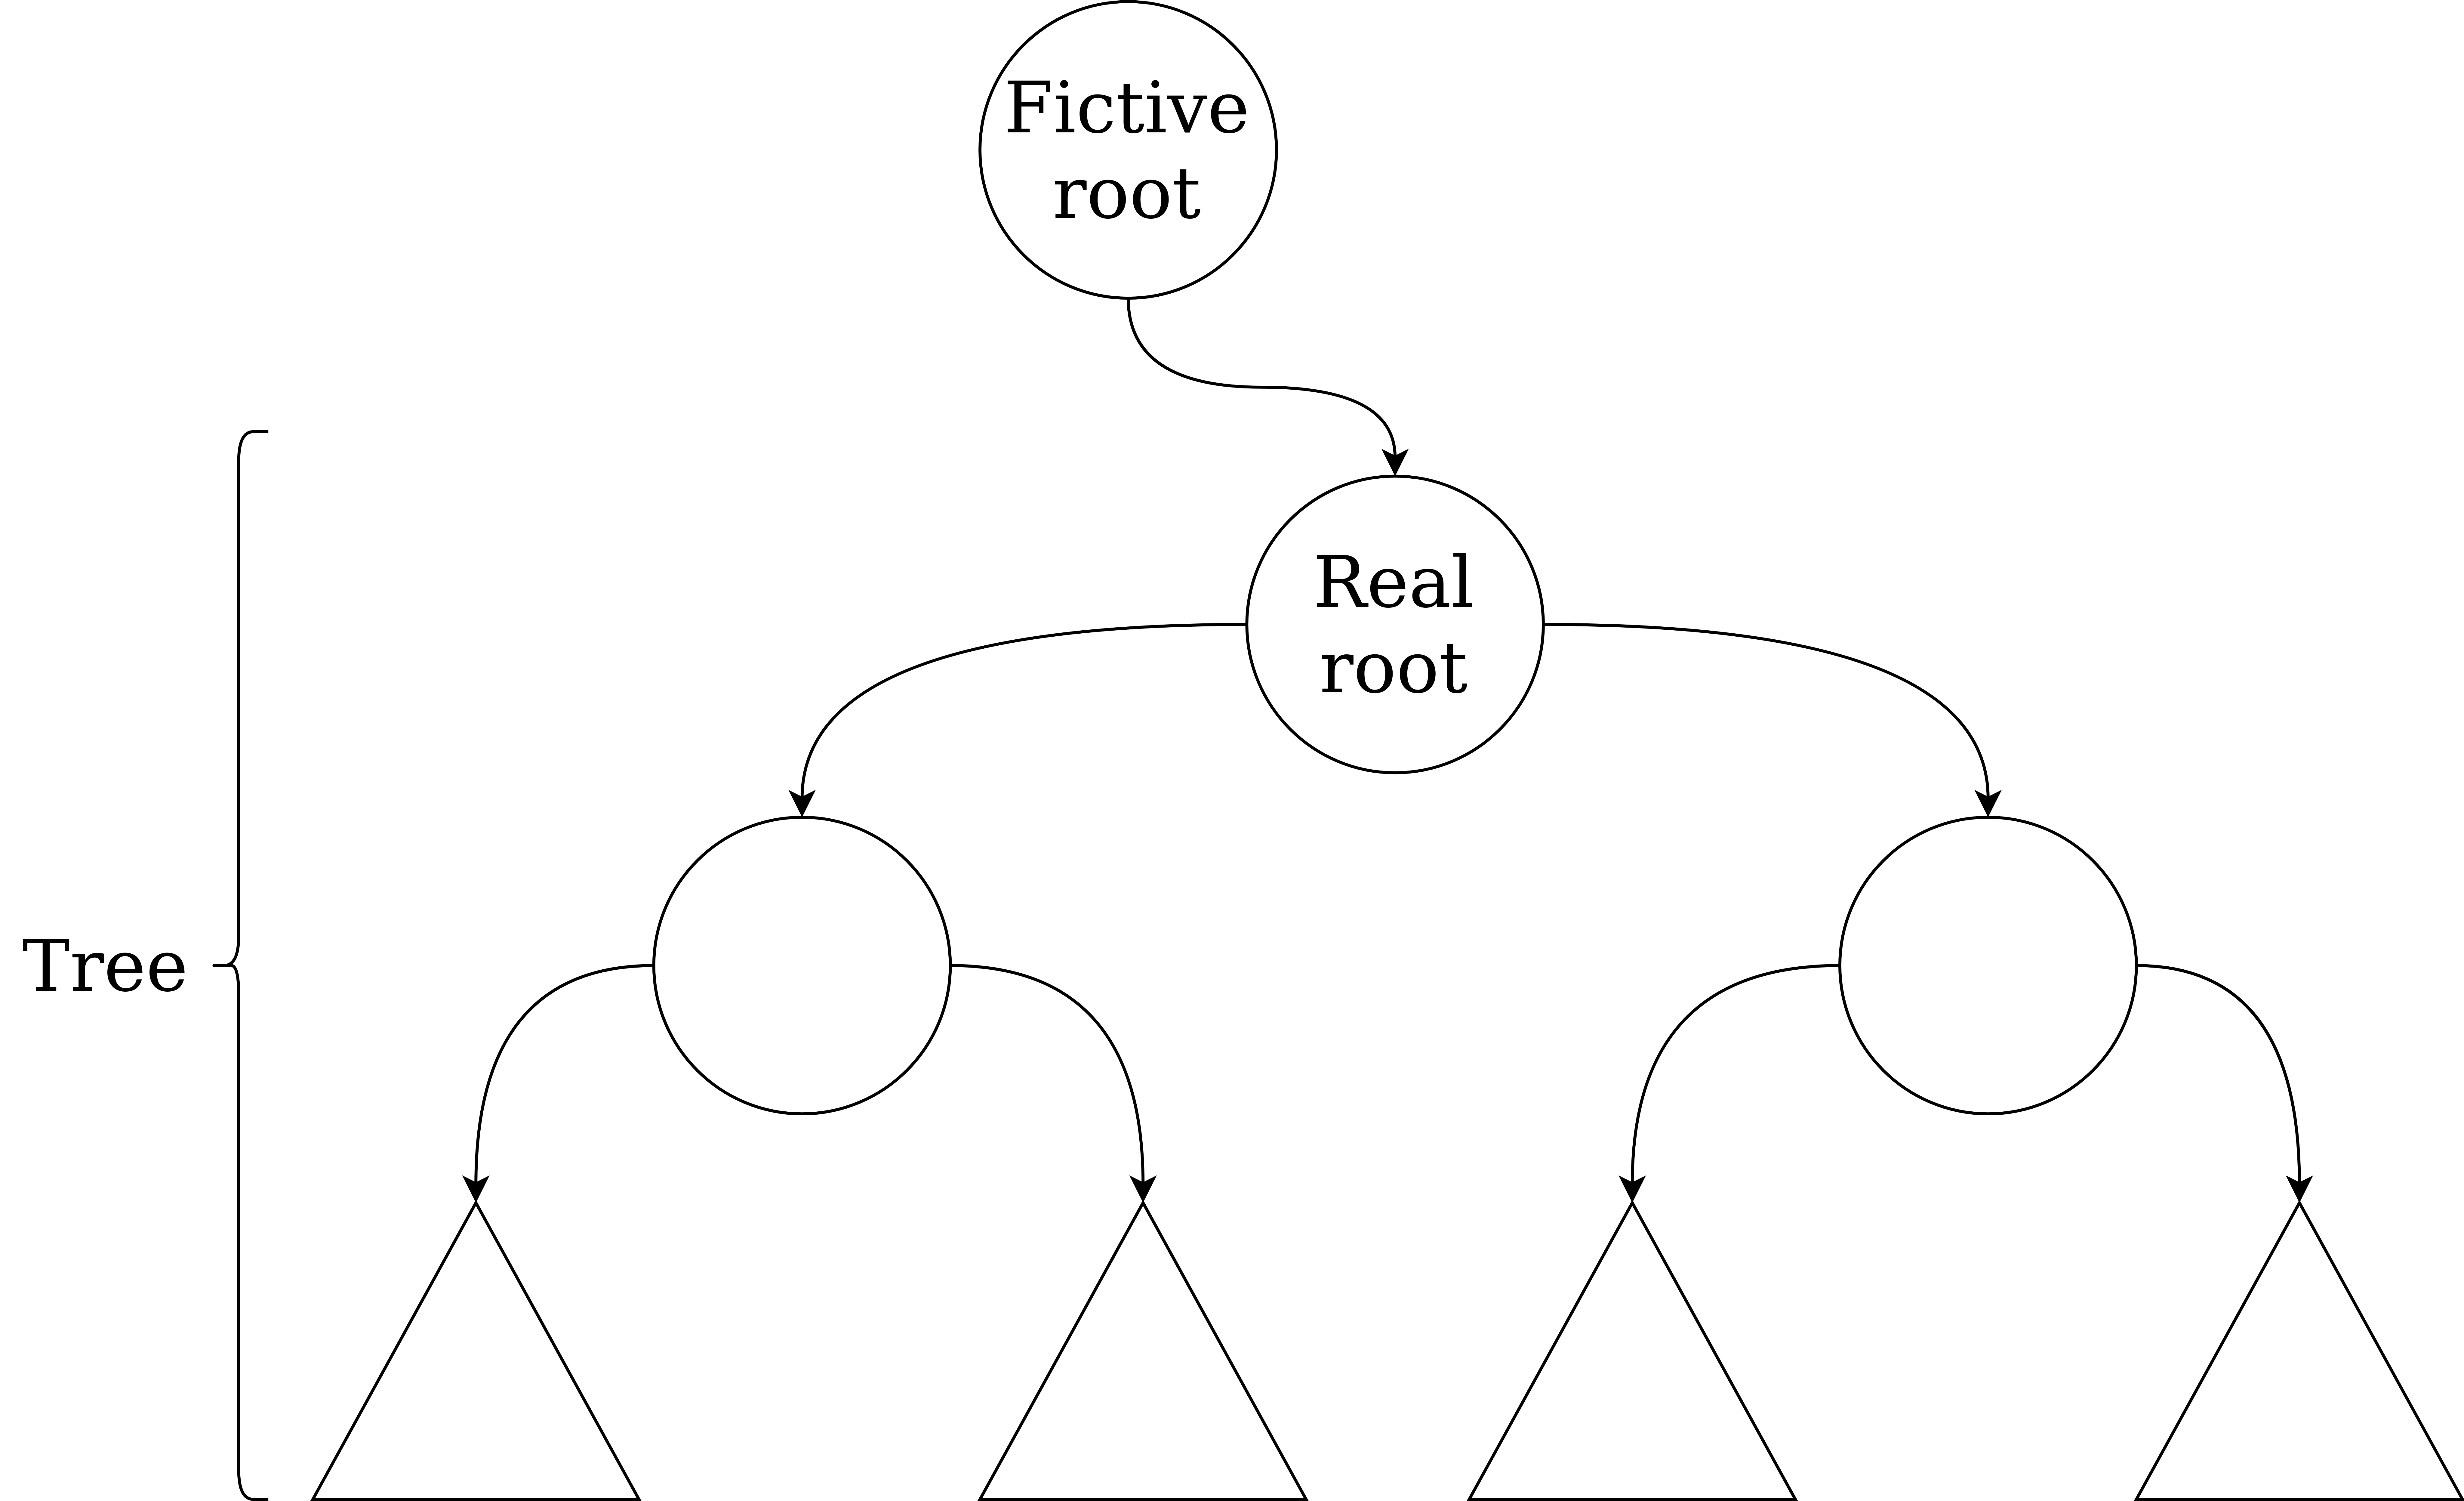
\includegraphics[width=\linewidth]{pics/fictive-root.png}
\end{figure}


In the latter sections we will describe, how an operation \texttt{Op} can be executed in a node \texttt{v}: either by using \texttt{CAS-N} (Section~\ref{casn-section})  or without it (Section~\ref{no-casn-chapter}).

Since we allow processes help each other, operation \texttt{Op}, initiated by process \texttt{P}, in any node \texttt{v} can be executed by some other (helper) process. Thus, we need to provide a mechanism for the process \texttt{P} by which it distinguishes between the two following situations:

\begin{itemize}
    \item Operation \texttt{Op} has not yet been executed in node \texttt{v}. Thus, the descriptor of \texttt{Op} is still located somewhere in \texttt{v} queue. In that case, \texttt{P} needs to continue executing operations from the head of \texttt{v} queue in node \texttt{v}.
    
    \item Operation \texttt{Op} has already been executed in node \texttt{v}. In that case, \texttt{P} can proceed to execute \texttt{Op} in lower nodes from the subtree of \texttt{v}.
\end{itemize}

\bigbreak

We can use timestamps to distinguish between these two situations. We describe that usage of timestamps with formulating and proving \emph{timestamps increasing property}. 

\begin{theorem}
In each queue, operation timestamps form a monotonically increasing sequence. More formally, if at any moment we traverse any queue \texttt{Q} from the head to the tail and obtain $\texttt{t}_{\texttt{1}}, \texttt{t}_{\texttt{2}}, \ldots \texttt{t}_{\texttt{n}}$~--- a sequence of timestamps of descriptors, located in \texttt{Q}, then $\texttt{t}_{\texttt{1}} < \texttt{t}_{\texttt{2}} < \ldots < \texttt{t}_{\texttt{n}}$ will hold.
\end{theorem}

\begin{proof}
We prove the theorem by the induction on the tree structure. As the induction basis, we will show that the statement holds for the tree root. As the induction step, we will prove that, given that the statement holds for some node \texttt{pv}, the statement holds for \texttt{v}~--- an arbitrary child of \texttt{pv}. Thus, the statement is guaranteed to hold for each tree node.

\begin{itemize}
    \item As requested in Section~\ref{main-invariant-chapter} and as explained in Section~\ref{push-acquire-timestamp-section}, the root queue provides timestamp allocation mechanism with the following guarantees: if descriptor of operation \texttt{A} is inserted to the root queue before descriptor of operation \texttt{B}, then \texttt{timestamp(A) < timestamp(B)} holds. Thus, the induction base is proven.
    
    \item Consider non-root node \texttt{v} and its parent \texttt{pv}. According to the induction assumption, the statement holds for \texttt{pv}. Thus, at \texttt{pv} queue descriptor timestamps form a monotonically increasing sequence: $\texttt{t}_{\texttt{1}} < \texttt{t}_{\texttt{2}} < \ldots < \texttt{t}_{\texttt{n}}$. Consider descriptors $\texttt{D}_{\texttt{i}}$ and $\texttt{D}_{\texttt{j}}$ (Fig.~\ref{timstamps-increasing-proof-pic}), such that:
    
    \begin{itemize}
        \item Both $\texttt{D}_{\texttt{i}}$ and $\texttt{D}_{\texttt{j}}$ should continue their execution at \texttt{v};
        \item \texttt{timestamp($\texttt{D}_{\texttt{i}}$) = $\texttt{t}_{\texttt{i}}$};
        \item \texttt{timestamp($\texttt{D}_{\texttt{j}}$) = $\texttt{t}_{\texttt{j}}$};
        \item $\texttt{D}_{\texttt{i}}$ is located closer to the head of \texttt{pv} queue than $ \texttt{D}_{ \texttt{j}}$ (therefore, $\texttt{D}_{\texttt{i}}$ was inserted to \texttt{pv} queue prior to $\texttt{D}_{\texttt{j}}$)~--- thus according to the induction assumption $\texttt{t}_{\texttt{i}} < \texttt{t}_{\texttt{j}}$.
    \end{itemize}
    
    \begin{figure}[H]
      \centering
      \caption{Descriptor $\texttt{D}_{\texttt{i}}$ is located closed to the head of \texttt{pv} queue than $\texttt{D}_{\texttt{j}}$, both $\texttt{D}_{\texttt{i}}$ and $\texttt{D}_{\texttt{j}}$ will continue their execution in \texttt{v} subtree}
      \label{timstamps-increasing-proof-pic}
      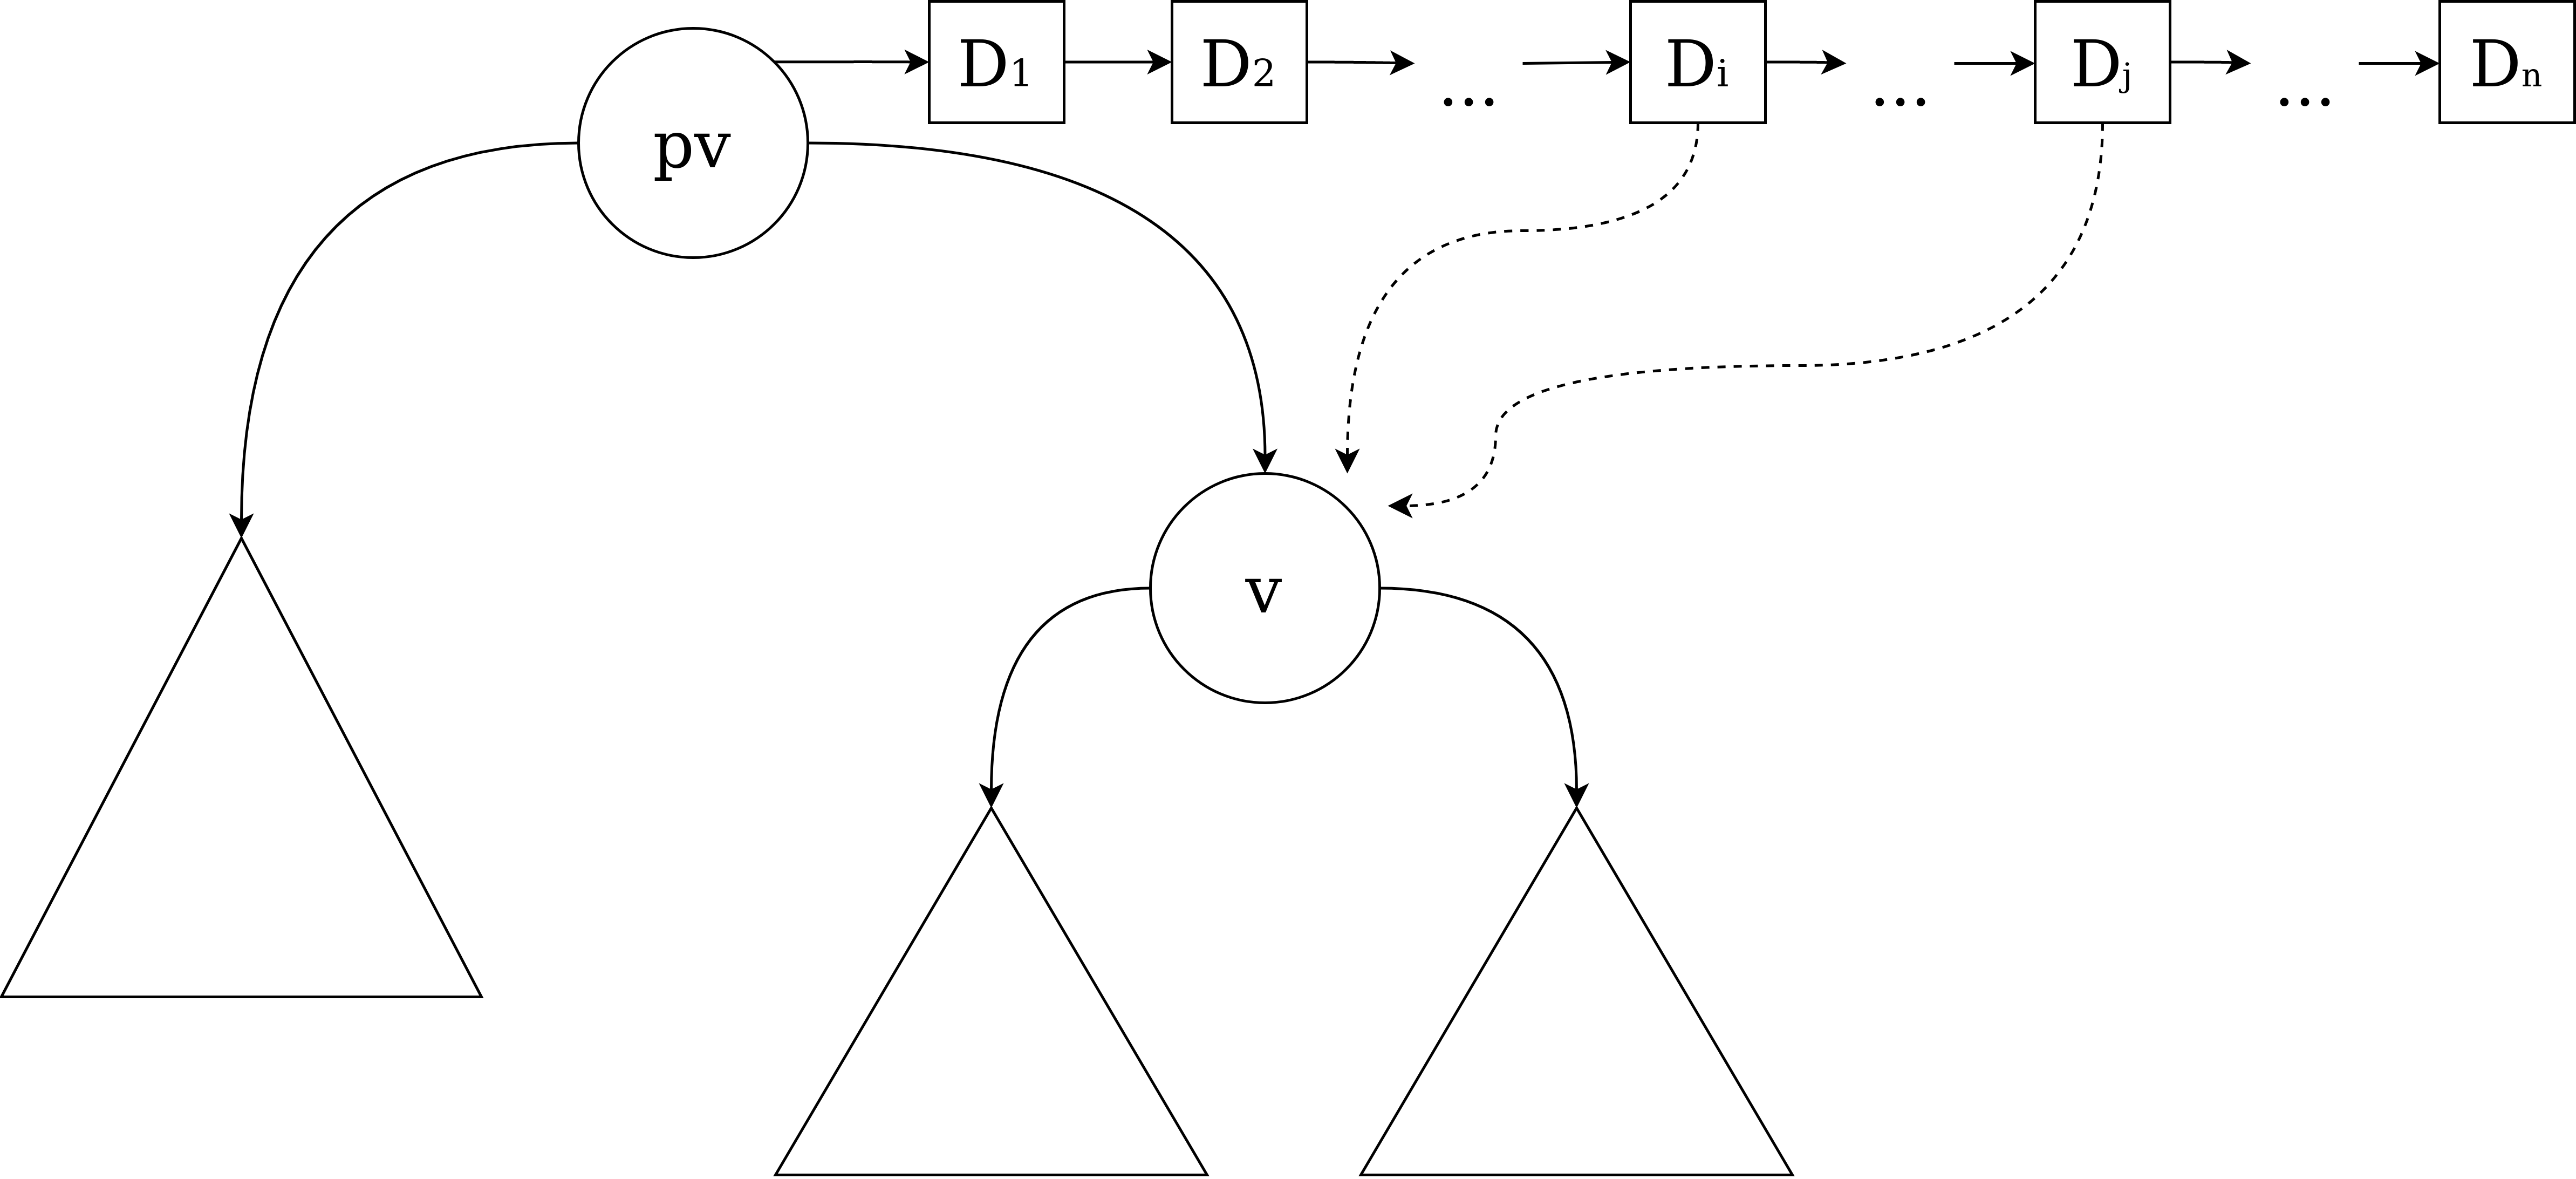
\includegraphics[width=\linewidth]{pics/timstamps-increasing-proof.png}
    \end{figure}
    
    In that case, according to the algorithm, the execution of $\texttt{D}_{\texttt{j}}$ in \texttt{pv} cannot begin until the the execution of $\texttt{D}_{\texttt{i}}$ in \texttt{pv} is finished. Since the execution of $\texttt{D}_{\texttt{i}}$ in \texttt{pv} includes inserting $\texttt{D}_{\texttt{i}}$ into \texttt{v} queue, the execution of $\texttt{D}_{\texttt{j}}$ in \texttt{pv} cannot begin until $\texttt{D}_{\texttt{i}}$ is inserted into \texttt{v} queue. Thus, $\texttt{D}_{\texttt{i}}$ is inserted into \texttt{v} queue prior to $\texttt{D}_{\texttt{j}}$, thus the timestamps increasing property holds for \texttt{v}.
\end{itemize}
\end{proof}

\bigbreak

As follows from that property, the initiator process \texttt{P} can easily learn, whether its operation \texttt{Op} has been executed in node \texttt{v} by using the following algorithm:

\begin{nenum}
    \item Try to read \texttt{head\_descriptor}~--- the descriptor, located at the head of \texttt{v} queue.
    
    \item If the queue is empty, we conclude that some other process has executed \texttt{Op} in node \texttt{v}. Thus, \texttt{P} continues traversing the tree, trying to execute \texttt{Op} at other nodes.
    
    \item Otherwise, \texttt{P} examines the timestamp of the obtained descriptor. If \texttt{head\_descriptor.Timestamp $>$ Op.Timestamp}, \texttt{P} yet again concludes, that some other process has executed \texttt{Op} at node \texttt{v}.
    
    \item Otherwise (\texttt{head\_descriptor.Timestamp $\leq$ Op.Timestamp}) \texttt{Op} is still located in \texttt{v} queue: either at the head (if \texttt{head\_descriptor.Timestamp $=$ Op.Timestamp}) or somewhere closer to the tail (if \texttt{head\_descriptor.Timestamp $<$ Op.Timestamp}). In that case, \texttt{P} executes the operation, denoted by \texttt{head\_descriptor} at node \texttt{v}.
\end{nenum}

\bigbreak

Therefore, we can implement the algorithm of executing all operations, up to \texttt{Op.Timestamp}, from \texttt{v} queue the following way (Listing~\ref{execute-until-timestamp-listing}):

\renewcommand{\lstlistingname}{Listing}
\begin{lstlisting}[caption={The algorithm to execute all operations, up to the specified timestamp \texttt{ts}, from \texttt{v} queue},label={execute-until-timestamp-listing},escapeinside={(*}{*)}, captionpos=b]
fun execute_until_timestamp(ts, v):
    while true:
        /*
        Queue.peek() returns the first descriptor in FIFO order
        */
        head_descriptor := v.Queue.peek()
        if head_descriptor = nil:
            return
        if head_descriptor.Timestamp > ts:
            return
        /*
        execute_in_node changes states of v children
        (in accordance with the operation, denoted by head_descriptor), 
        pushes head_descriptor to child queues, 
        removes head_descriptor from v queue 
        */
        execute_in_node(head_descriptor, v)
\end{lstlisting}

Also, we should have a method to determine whether the operation execution has been finished or not. The motivation to introduce such a method is the following situation:

\begin{nenum}
    \item Process \texttt{P} starts executing operation \texttt{Op}.
    
    \item \texttt{P} inserts descriptor of \texttt{Op} to the root queue.
    
    \item \texttt{P} is suspended by the OS.
    
    \item Other processes finish the execution of \texttt{Op}.
    
    \item After being resumed by the OS, \texttt{P} should be able to learn, whether \texttt{Op} has already been executed or not.
\end{nenum}

\bigbreak

We shall implement this capability by storing \emph{result pointer} in each operation descriptor (Fig.~\ref{descriptor-internals-pic}). This pointer will point to a specific memory location that stores either the operation result (if the operation execution has been already finished~--- in that case \texttt{P} can return that result to the caller) or \texttt{nil} (if the operation execution has not been finished yet~--- in that case \texttt{P} should continue traversing the tree and finish \texttt{Op} execution).

\begin{figure}[H]
  \centering
  \caption{A glance into a descriptor internals: each descriptor contains at least operation type (e.g. \texttt{insert}, \texttt{remove}, \texttt{count}), operation arguments (e.g., a key to insert or remove) and the result pointer}
  \label{descriptor-internals-pic}
  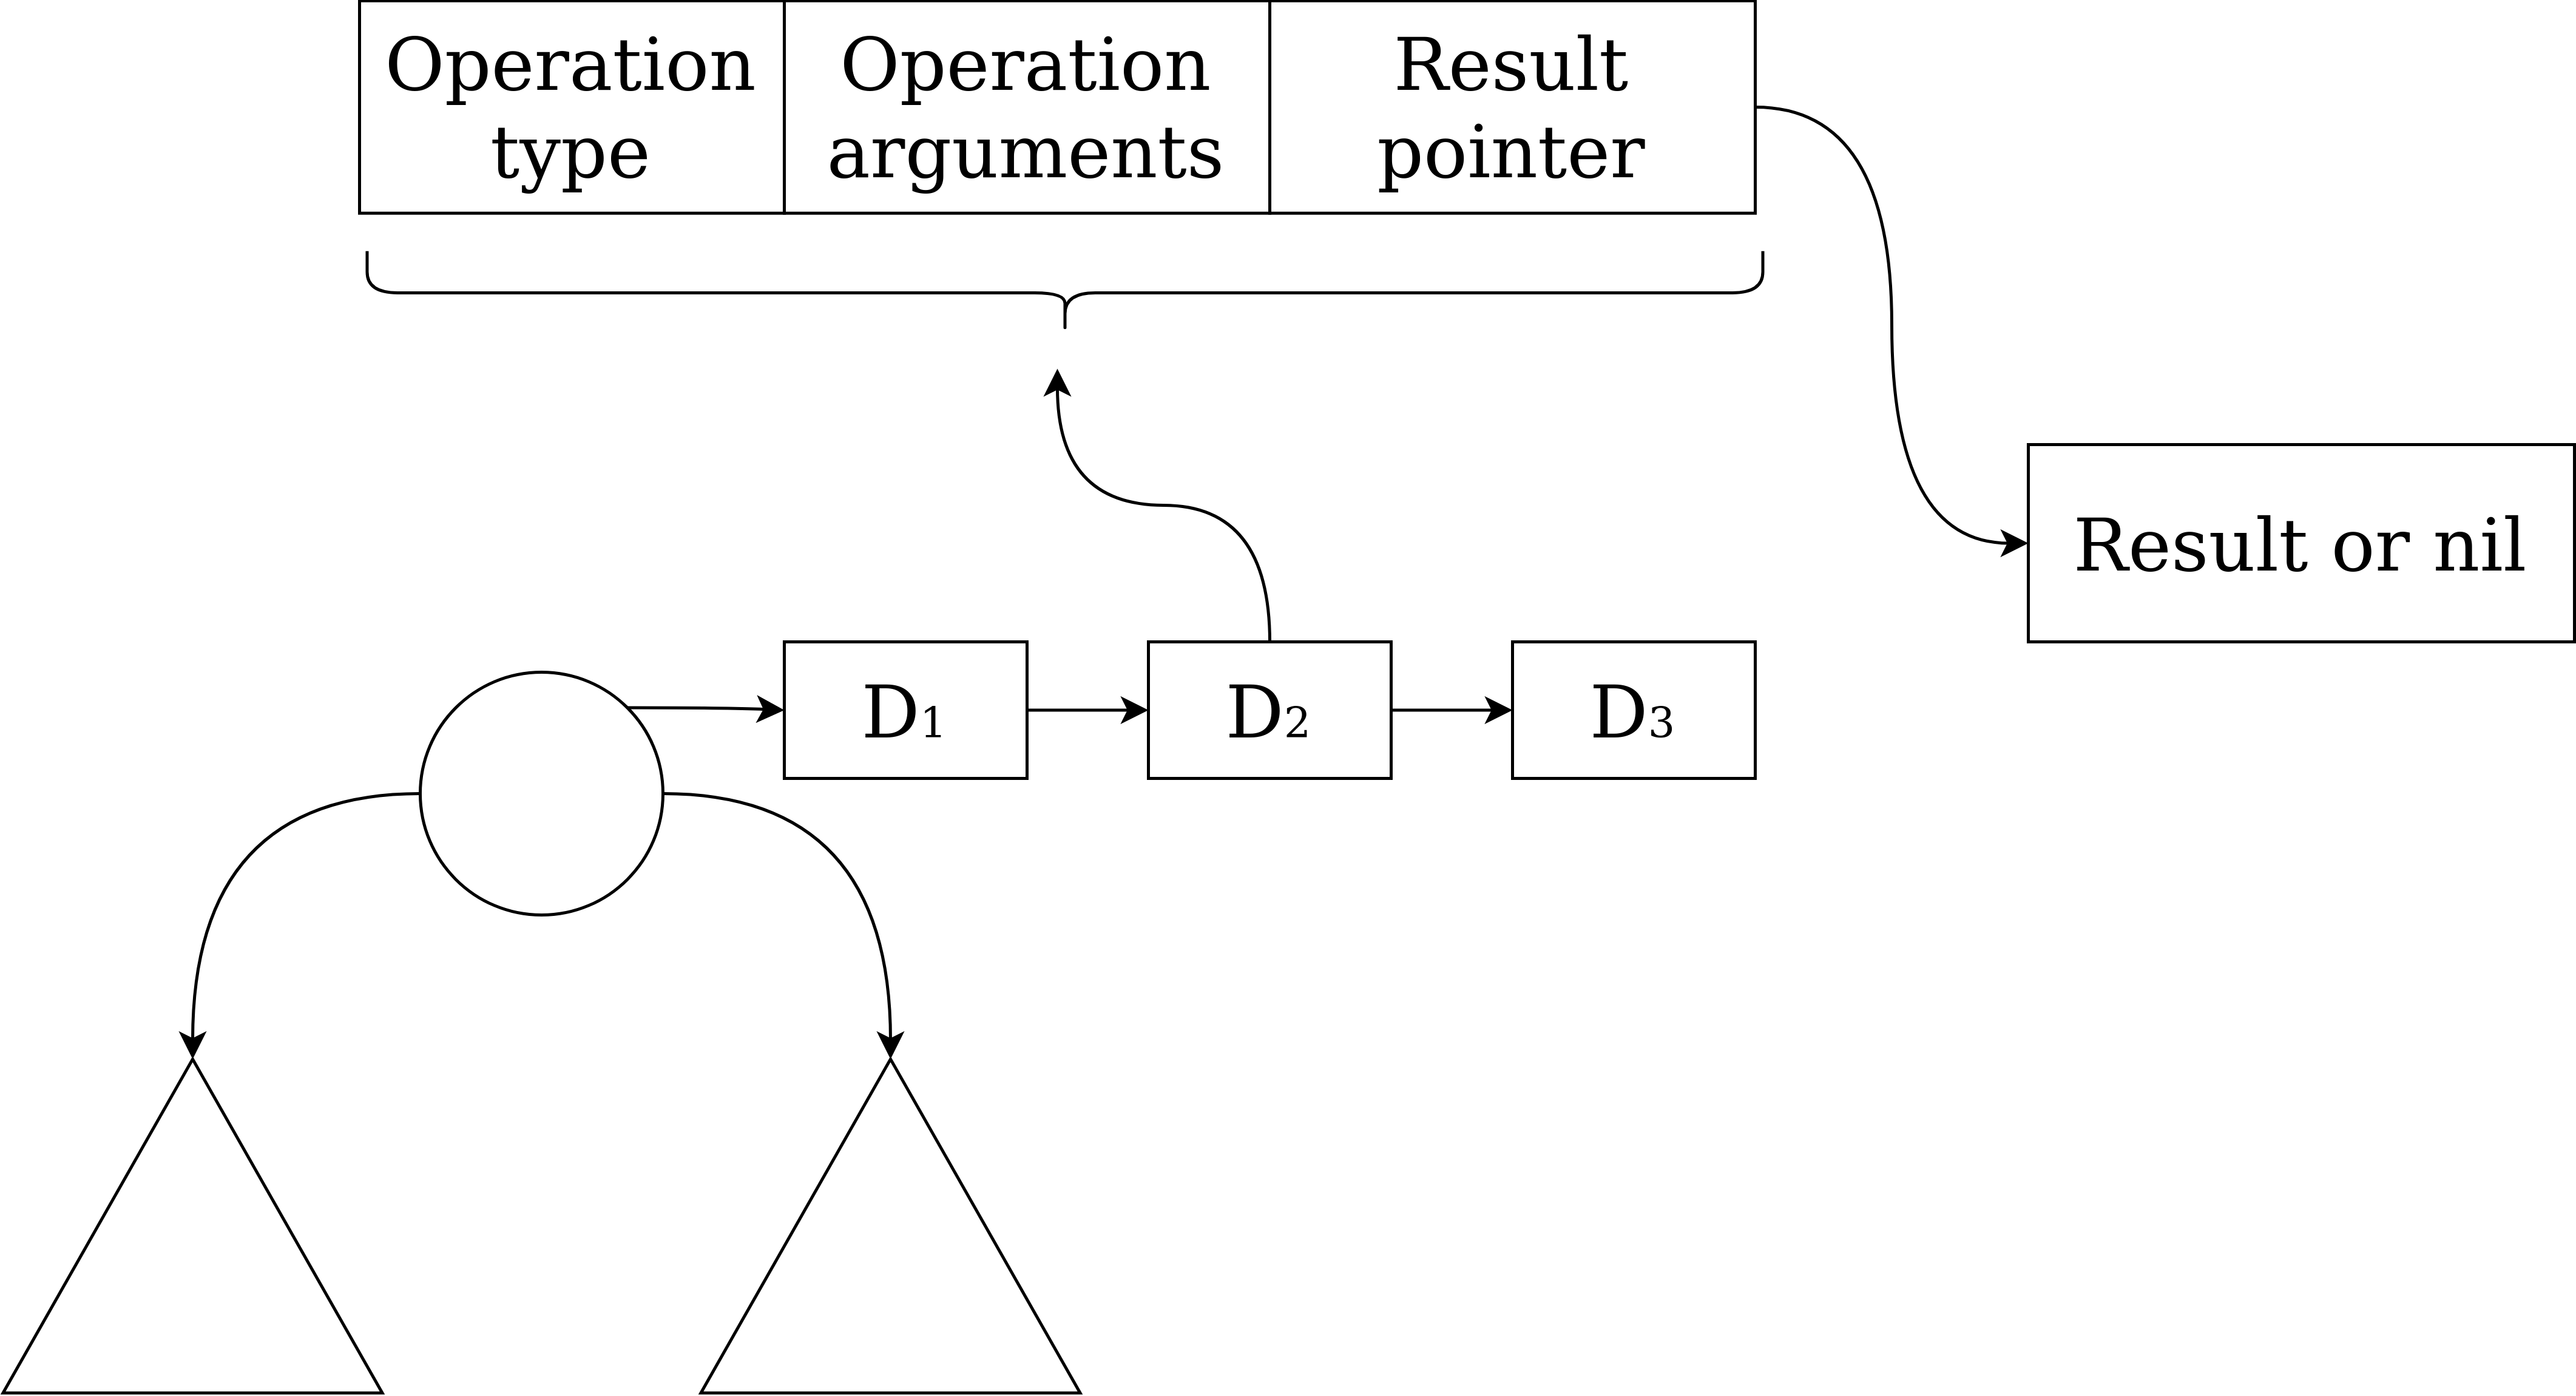
\includegraphics[width=\linewidth]{pics/descriptor-internals.png}
\end{figure}

\section{Ways to achieve parallelism}

As was stated in Section~\ref{main-invariant-chapter}, operations should be applied to the tree in
the order, their descriptors were added to the root descriptor queue. Therefore, one can wonder: how can we achieve parallelism, while linearizing all operations via the root queue? It seems, that our proposed solution is not better than the solutions, based on the Universal Construction (see Section~\ref{universal-constrcution-section} for discussion on drawbacks of such solutions). Our scheme has one major advantage over the Universal Construction. As we remember, in solutions, based on the Universal Construction, execution of modifying operation $O_2$ could be started only after the execution of modifying operation $O_1$ has been finished~--- otherwise, one of these operations faces unsuccessful \texttt{CAS} and has to retry. In contrast, in our solution, two successful modifying operations may be executed in parallel if they are executed on different subtrees (Fig.~\ref{paralellism-how-pic}). 

\begin{figure}[H]
  \centering
  \caption{After being routed to different subtrees, modifying operations $O_1$ and $O_2$ may be executed in parallel, in contrast to the Universal Construction-based solutions}
  \label{paralellism-how-pic}
  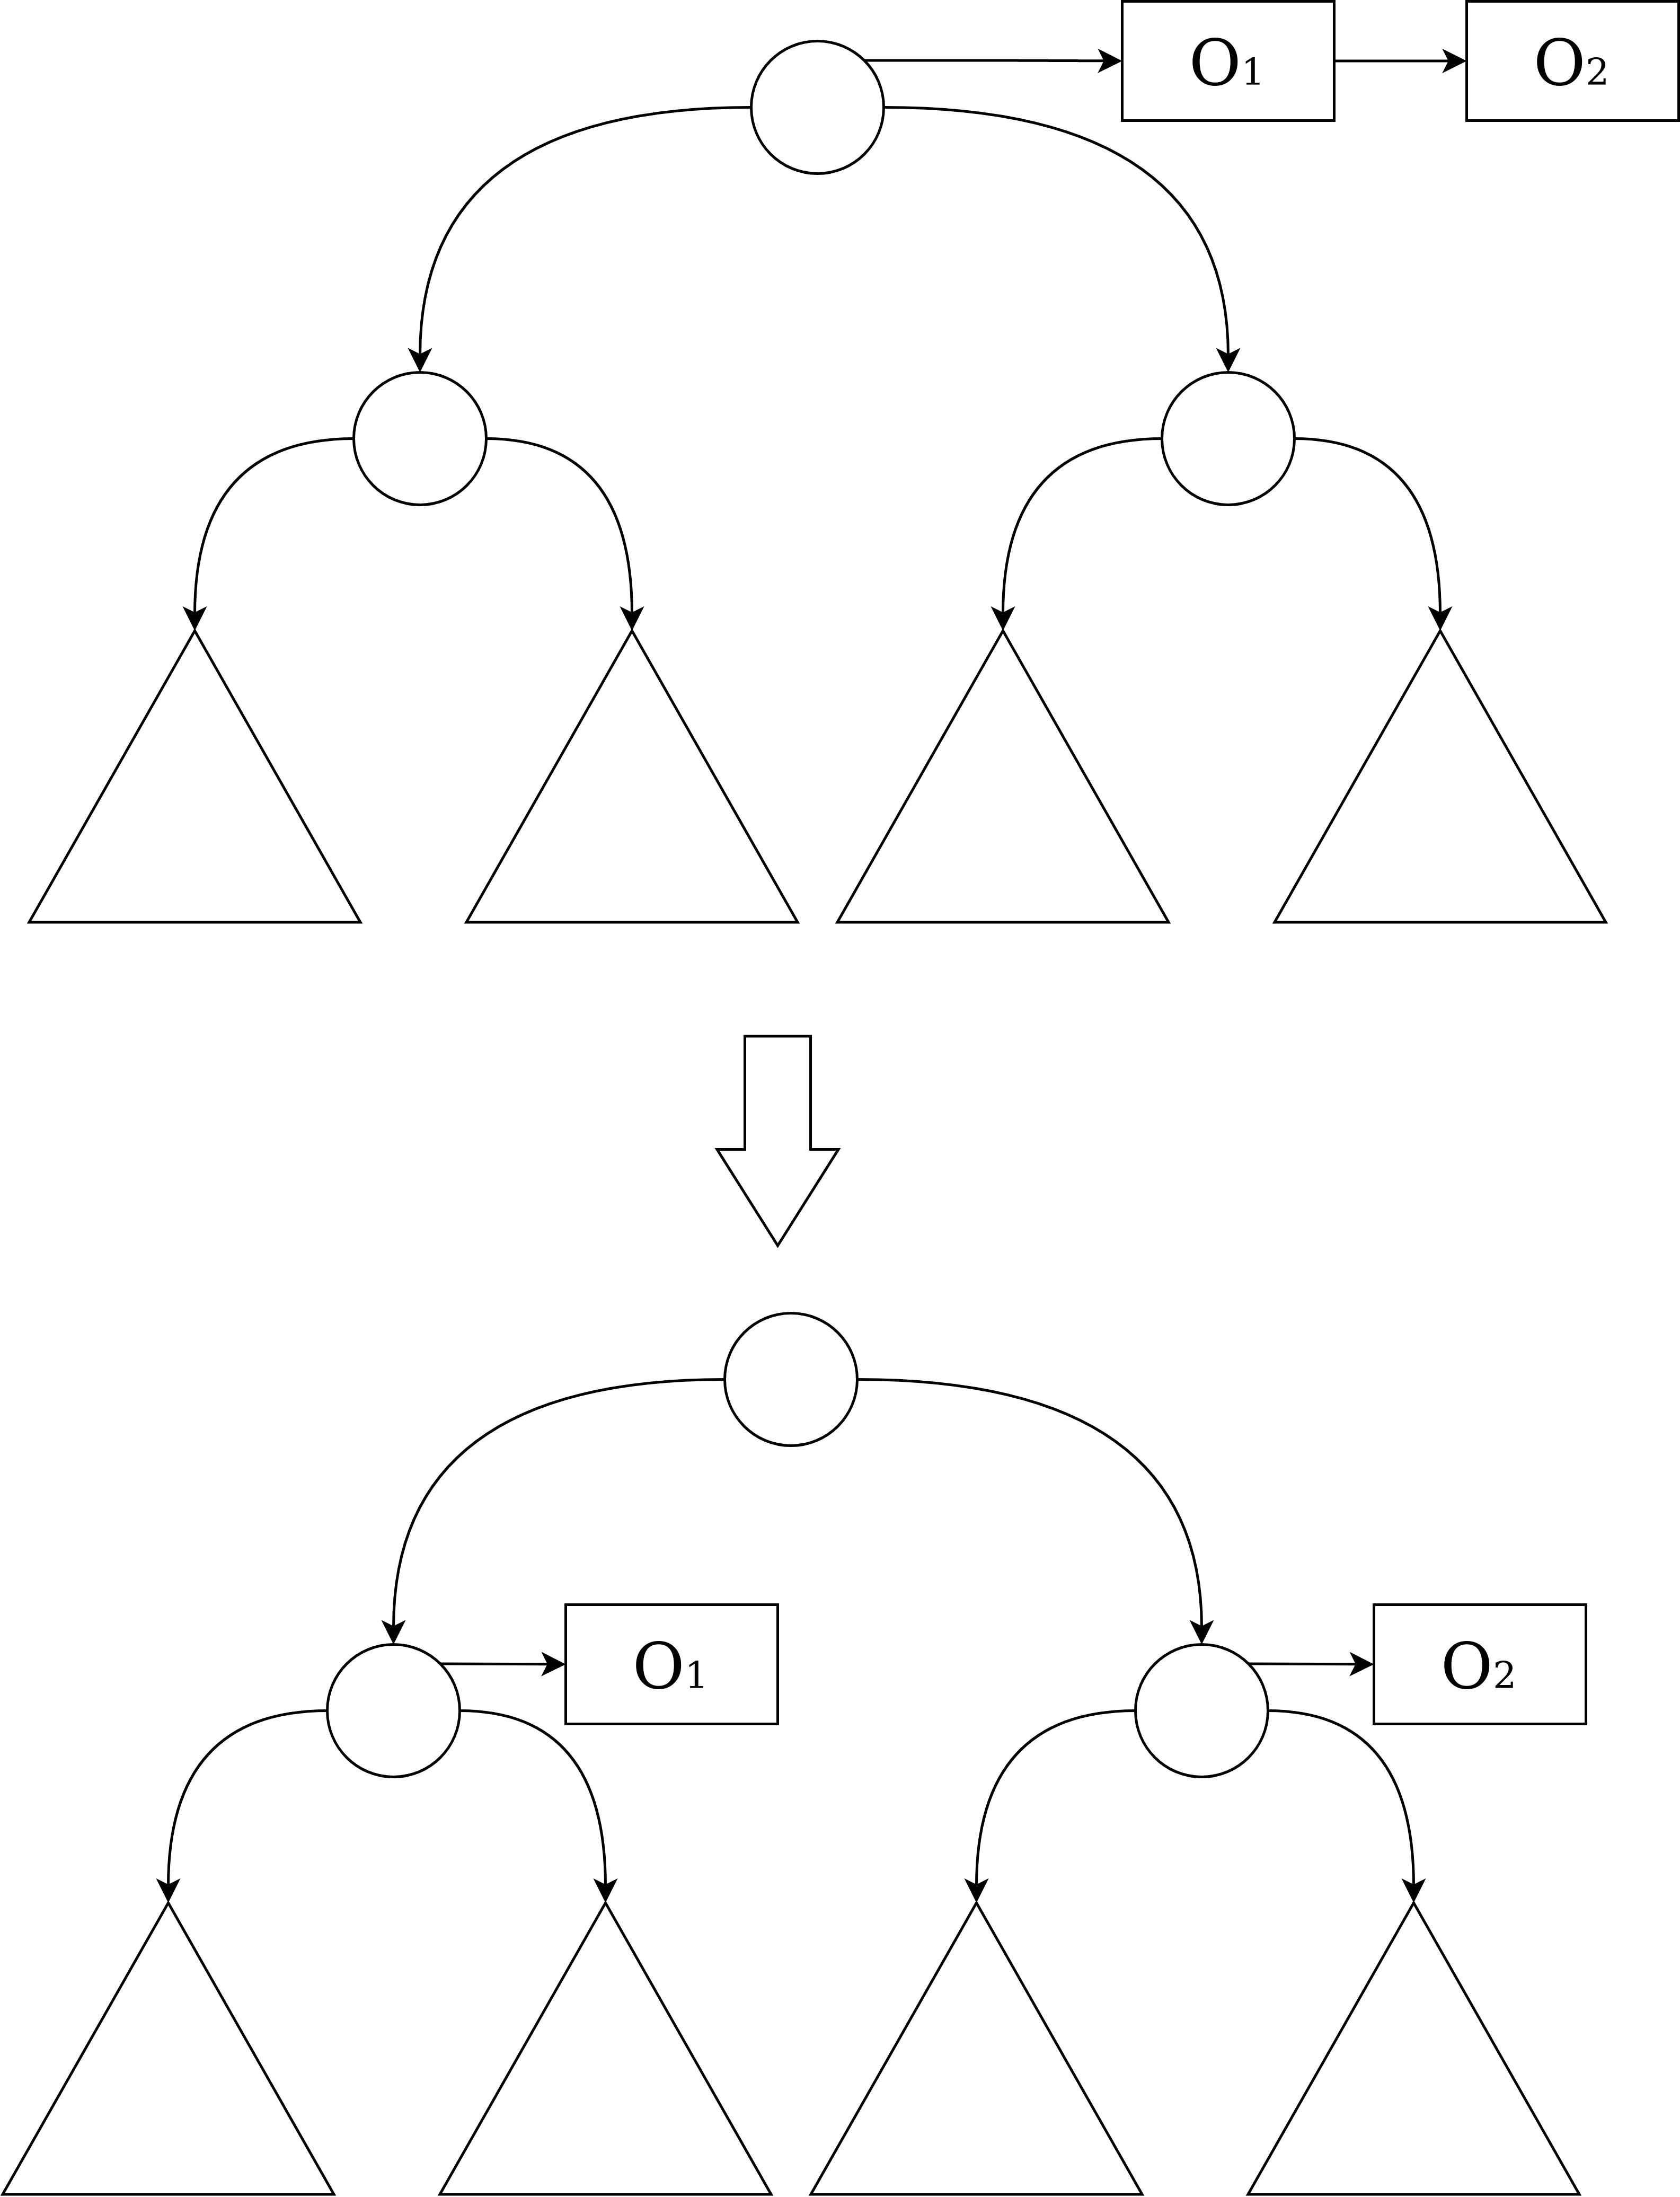
\includegraphics[width=\linewidth]{pics/paralellism-how.png}
\end{figure}

Note that a particular execution order, determined by the queue, is enforced only in the root node~--- in the root node we execute $O_1$ before starting executing $O_2$. At lower tree levels, we do not enforce a particular execution order. This can be achieved because at lower tree levels $O_1$ and $O_2$ do not conflict with each other anymore, since they operate on different subtrees. Thus, our logical order (in which $O_1$ precedes $O_2$) does not require us to enforce a particular physical execution order on these operations, i.e., executing $O_1$ before starting executing $O_2$.

\section{Executing an operation in a node via \texttt{CAS-N}}
\label{casn-section}

\subsection{\texttt{CAS-N} definition and implementation}
\label{cas-n-definition}

\texttt{CAS-N} is a powerful concurrent primitive that takes \texttt{N} registers, \texttt{N} expected values, and \texttt{N} new values as an input. After that, it atomically checks, whether $\forall i \in [1 \ldots N] : $ value of \texttt{i}-th register equals to the \texttt{i}-th expected value. If so, it modifies values of all registers, so that the value of the \texttt{i}-th register becomes equal to the \texttt{i}-th new value, and returns \texttt{true}. Otherwise~--- if $\; \exists j \in [1 \ldots N] : $ value of \texttt{j}-th register does not equal to \texttt{j}-th expected value~--- it leaves all registers unmodified and returns \texttt{false}. The pseudocode of \texttt{CAS-N} is presented on Listing~\ref{cas-n-listing}:

\renewcommand{\lstlistingname}{Listing}
\begin{lstlisting}[caption={Pseudocode for \texttt{CAS-N} operation},label={cas-n-listing},escapeinside={(*}{*)}, captionpos=b]
fun multi_cas(n: int, Registers: [n]Register,
              expected_values: [n]Value, new_values: [n]Value):
    atomically:
        for i (*$\leftarrow$*) 1 .. n:
            v := Registers[i]
            if v (*$\neq$*) expected_values[i]:
                return false
        for i (*$\leftarrow$*) 1 .. n:
            Registers[i] (*$\leftarrow$*) new_values[i]
        return true
\end{lstlisting}

We can use \emph{Two-Phase Locking} protocol, described e.g., in~\cite{bernstein1987concurrency}, to implement \texttt{CAS-N} the following way (Listing~\ref{cas-n-lock-listing}):

\renewcommand{\lstlistingname}{Listing}
\begin{lstlisting}[caption={Two-phase lock-based implementation of \texttt{CAS-N}},label={cas-n-lock-listing},escapeinside={(*}{*)}, captionpos=b]
fun multi_cas(n: int, Registers: [n]Register, Locks: [n]Mutex, 
              expected_values: [n]Value, new_values: [n]Value):
    for i (*$\leftarrow$*) 1 .. n:
        Locks[i].lock()
        v := Registers[i]
        if v (*$\neq$*) expected_values[i]:
            for j (*$\leftarrow$*) 1 .. i:
                Locks[j].unlock()
            return false
    for i (*$\leftarrow$*) 1 .. n:
        Registers[i] (*$\leftarrow$*) new_values[i]
        Locks[i].unlock()
    return true
\end{lstlisting}

This implementation is lock-based, thus, it does not guarantee even the obstruction-freedom (see Section~\ref{section-guarantees} for discussion on concurrent progress guarantees). Moreover, it is prone to deadlocks~\cite{bernstein1987concurrency}~--- thus, the need for an implementation, not suffering from these drawbacks, arise. Harris et al.~\cite{harris2002practical} described software lock-free implementation of \texttt{CAS-N}. Feldman et al.~\cite{feldman2015wait} showed that there exists a practical wait-free implementation of \texttt{CAS-N}. For efficiency reasons, it is possible to implement special cases of \texttt{CAS-N} (e.g., \texttt{CAS-2}~\cite{cas-2-wiki}) in a hardware, making them wait-free and extremely efficient (e.g., since the hardware implementation does dot require dynamic memory allocation).

\subsection{Using \texttt{CAS-N} for operation execution}

As was discussed in Section~\ref{operation-execution-chapter}, execution of operation \texttt{Op} in node \texttt{v} consists of:

\begin{itemize}
    \item Modifying states of \texttt{v} children;
    \item Modifying \texttt{v} child queues~--- inserting \texttt{Op} descriptor into some of them;
    \item Modifying \texttt{v} queue~--- removing \texttt{Op} descriptor from its head;
\end{itemize}

\bigbreak

We can do it atomically using \texttt{CAS-N}. To allow atomic modification of queues with \texttt{CAS-N}, we shall employ persistent queues (Fig.~\ref{queue-cas-pic}). We can simply store a pointer to the current version of \texttt{node} persistent queue in \texttt{node.Q\_Ptr} register. After that, we can use \texttt{CAS(\&node.Q\_Ptr, cur\_queue, new\_queue)} or \texttt{CAS-N} to try to atomically modify the queue (see Section~\ref{universal-constrcution-section} for explanation on how \texttt{CAS} can be used to modify persistent data structures).

\begin{figure}[H]
  \centering
  \caption{Using \texttt{CAS} to atomically modify persistent queues}
  \label{queue-cas-pic}
  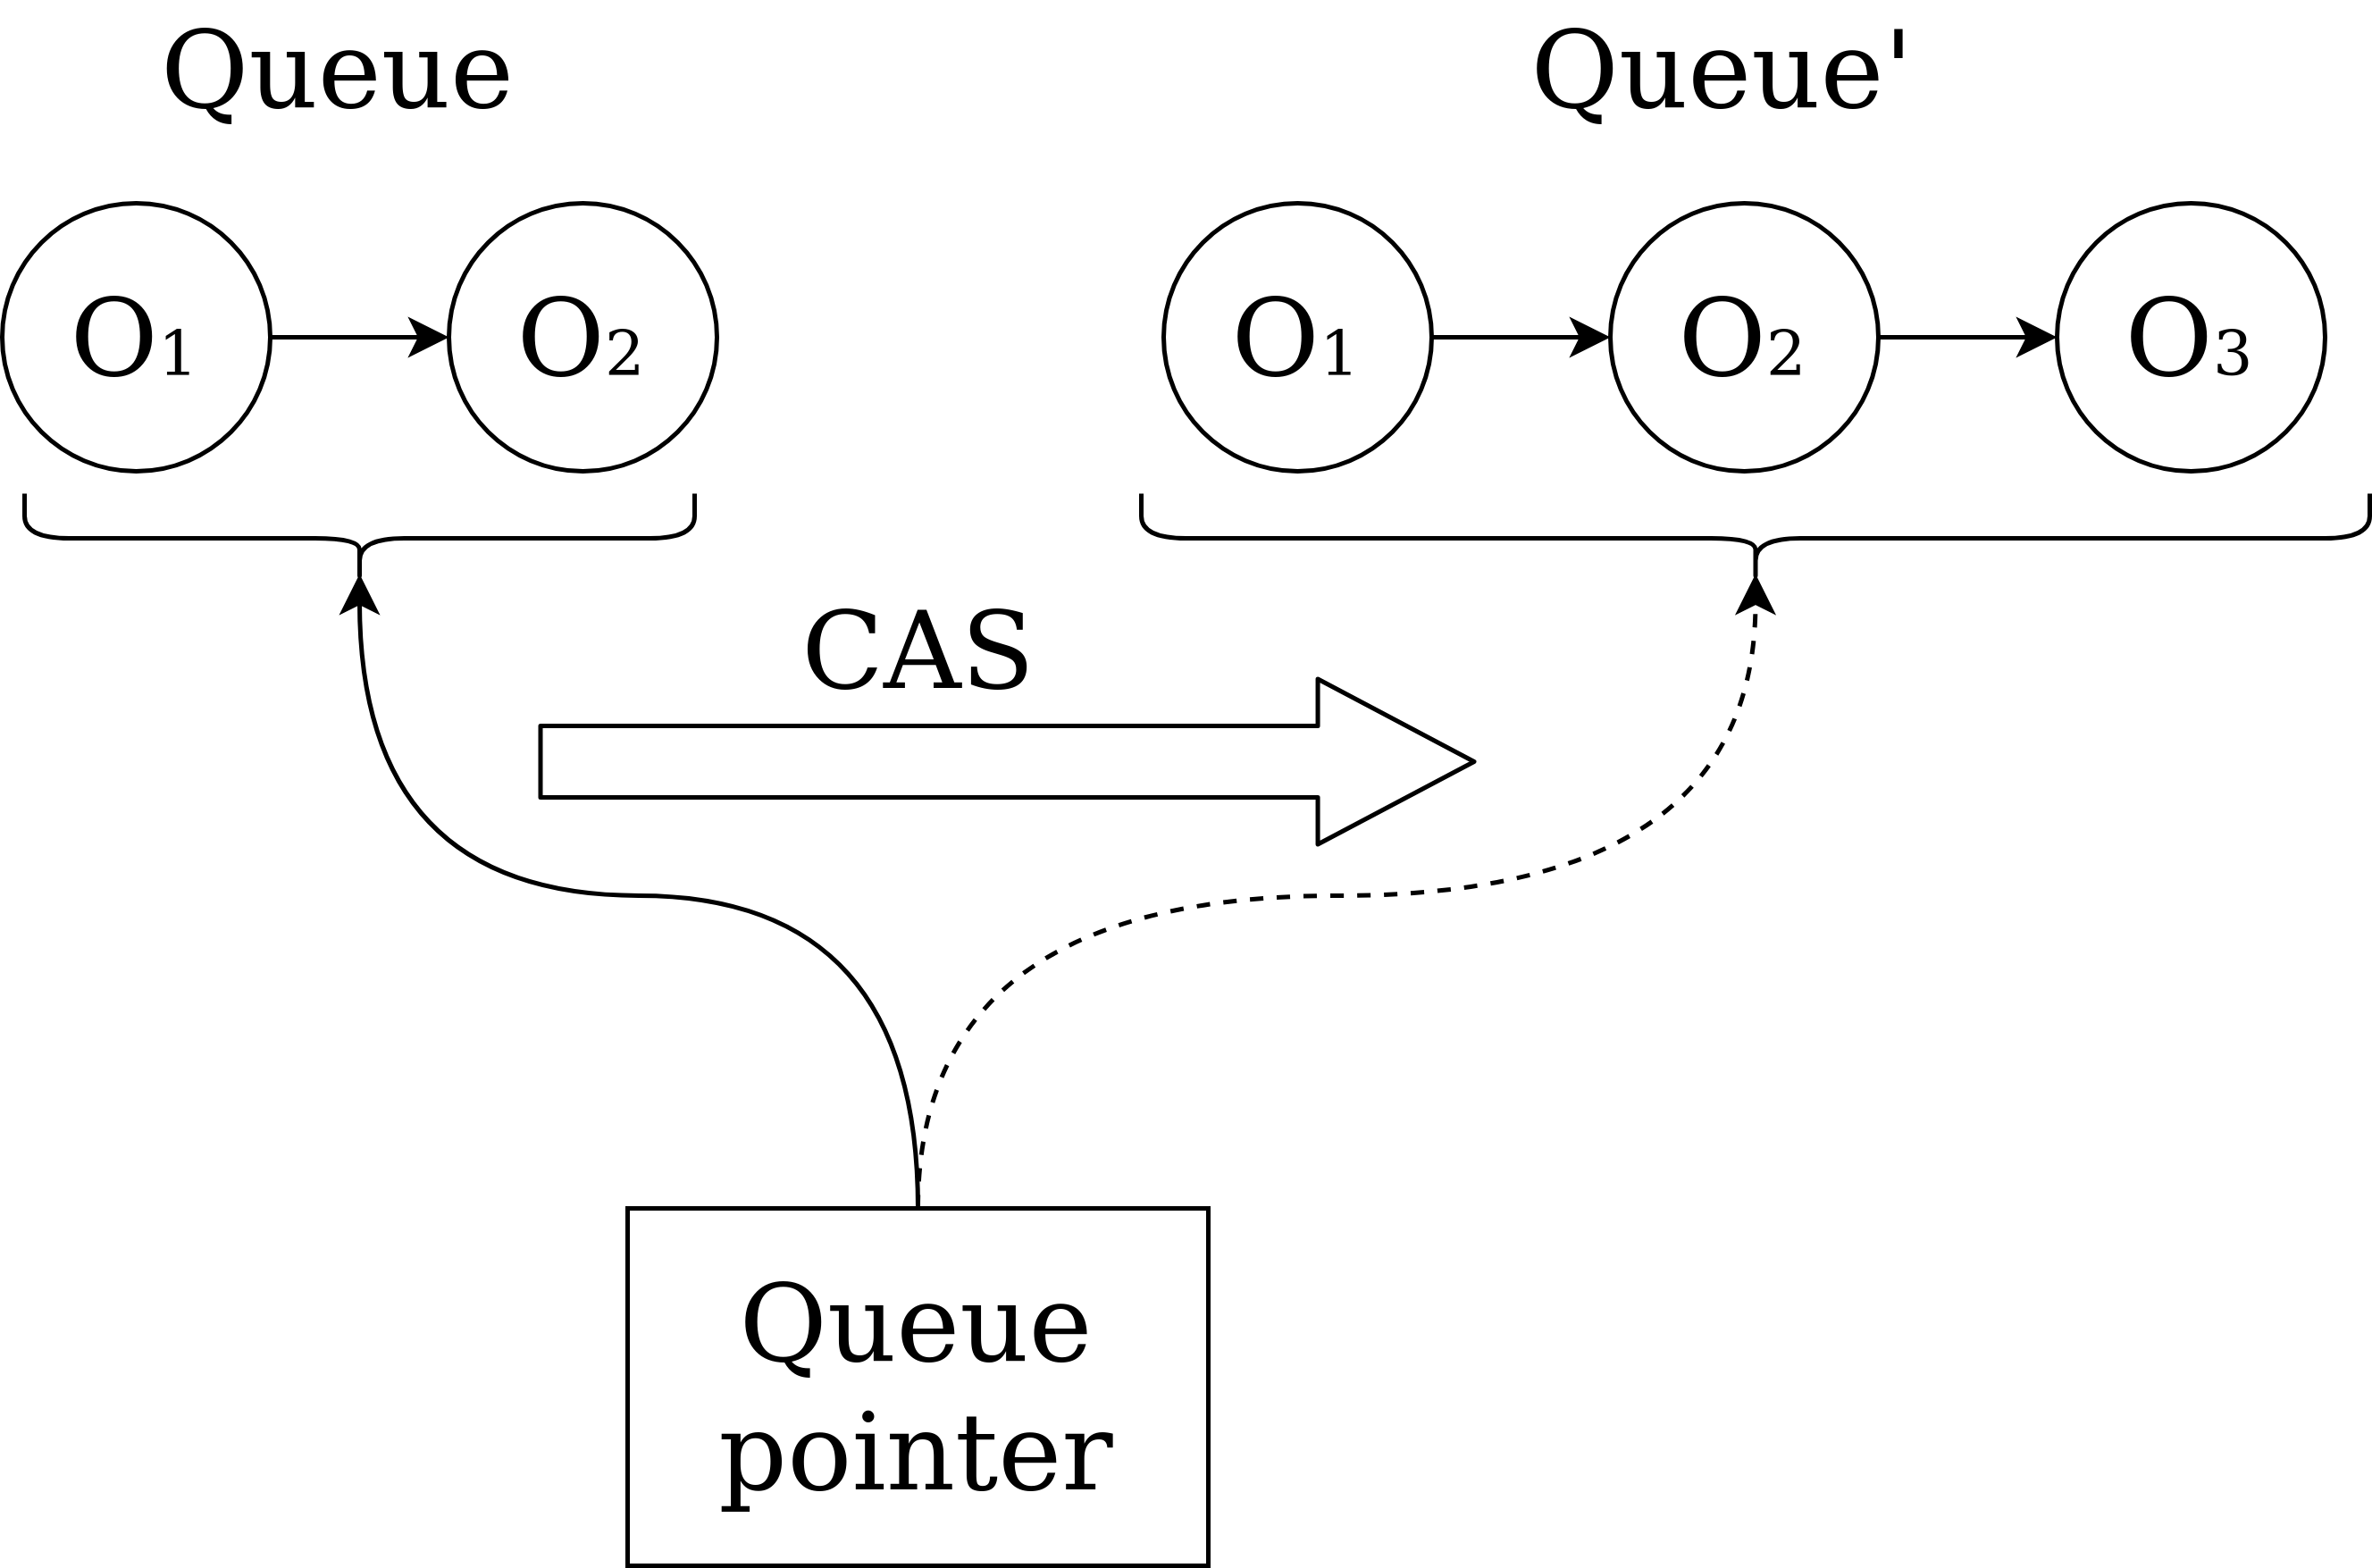
\includegraphics[width=\linewidth]{pics/queue-cas.png}
\end{figure}

Multiple persistent queues have been studied and described in the literature. Bankers queue~\cite{okasaki1999purely} is considered one of the fastest and the most memory-optimal.

Node state can be modified either: 1)~the same way as queues~--- via storing the current state in the heap and modifying the pointer to it located in the tree node (this method is described in more details in Section~\ref{no-casn-chapter}); 2)~directly in the tree node~--- each component of the state (e.g., subtree size) is located directly in the tree node and modified inplace. In the last case, \texttt{CAS-N} should be applied to each component of the state.

Therefore, we can use \texttt{CAS-N} to atomically modify all the necessary registers: child queue pointers, \texttt{v} queue pointer, and child states (Fig.~\ref{execution-casn-pic}).

\begin{figure}[H]
  \centering
  \caption{Using \texttt{CAS-N} to atomically modify child queues, parent queue, and child states in a binary tree. Here we store the node state in the heap and store \texttt{S\_Ptr}~--- a pointer to the node state~--- in the node. In that case, \texttt{CAS-5} is sufficient to modify all the required registers: both child queues, both child states and the parent queue}
  \label{execution-casn-pic}
  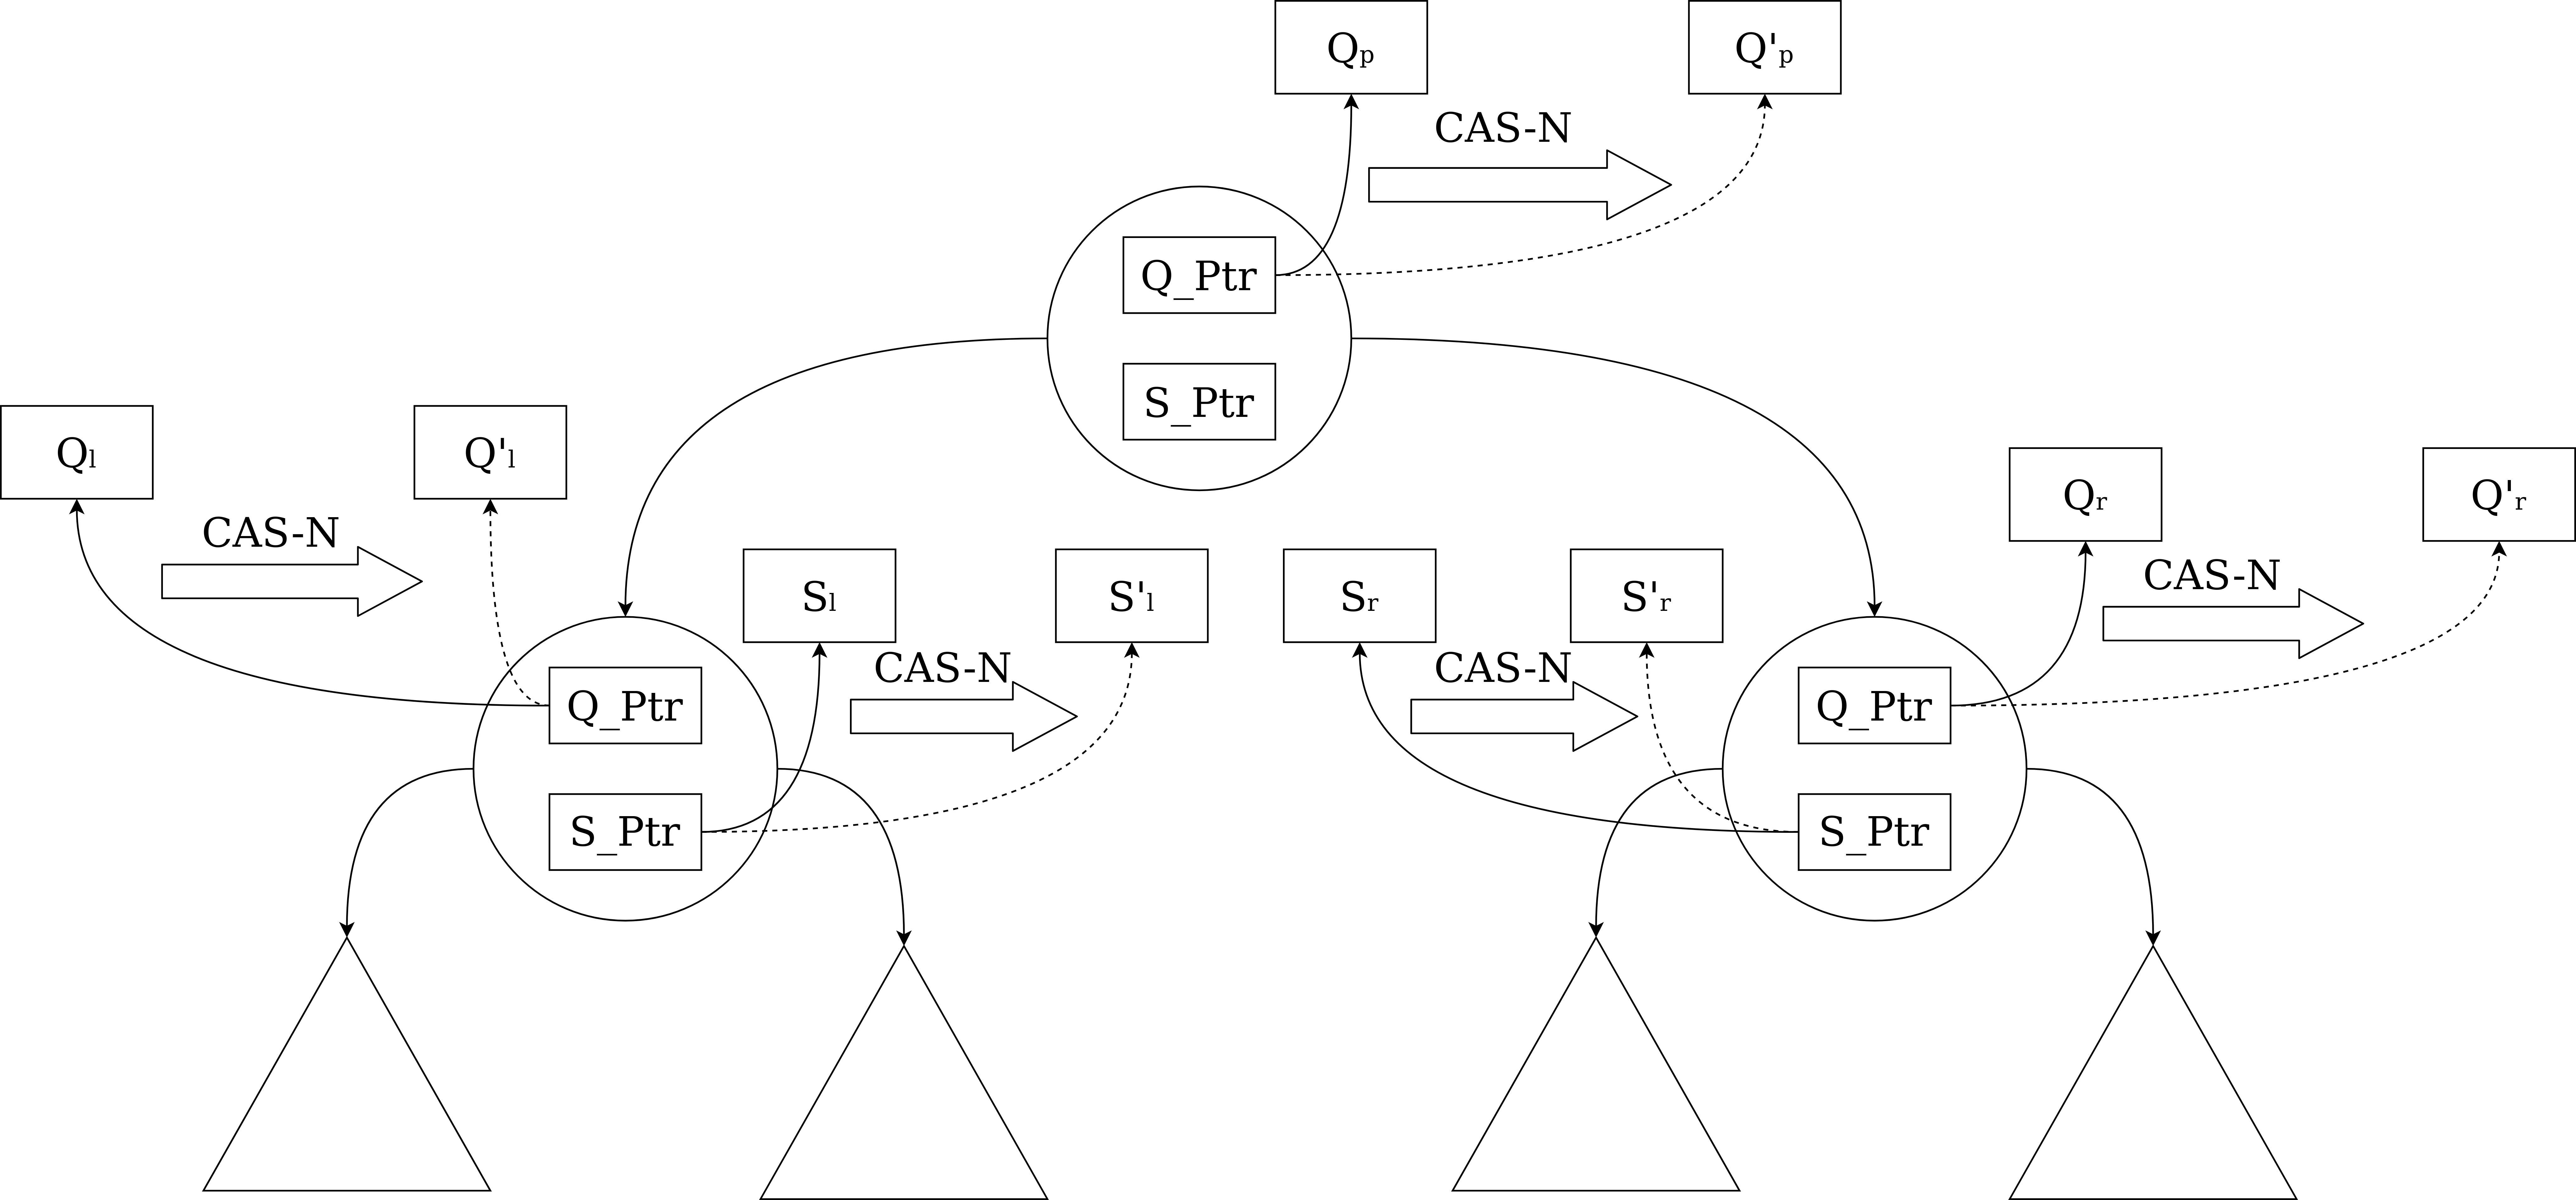
\includegraphics[width=\linewidth]{pics/execution-casn.png}
\end{figure}

If \texttt{CAS-N} returns \texttt{true} we conclude that we have successfully executed \texttt{Op} in node \texttt{v}. Otherwise, the \texttt{CAS-N} may return \texttt{false} because of any of the following two reasons (Fig~\ref{casn-fail-pic}): 

\begin{nenum}
    \item Other process has executed in node \texttt{v} the operation we are trying to execute, including removal of its descriptor from the head of \texttt{v} queue (Fig.~\ref{casn-fail-remove-pic}).
    
    \item Other process has inserted new operation descriptor to \texttt{v} queue, without executing in node \texttt{v} the operation we are trying to execute (Fig.~\ref{casn-fail-insert-pic}).
\end{nenum}

\begin{figure}[H]
     \centering
     \begin{subfigure}[b]{0.40\linewidth}
          \centering
          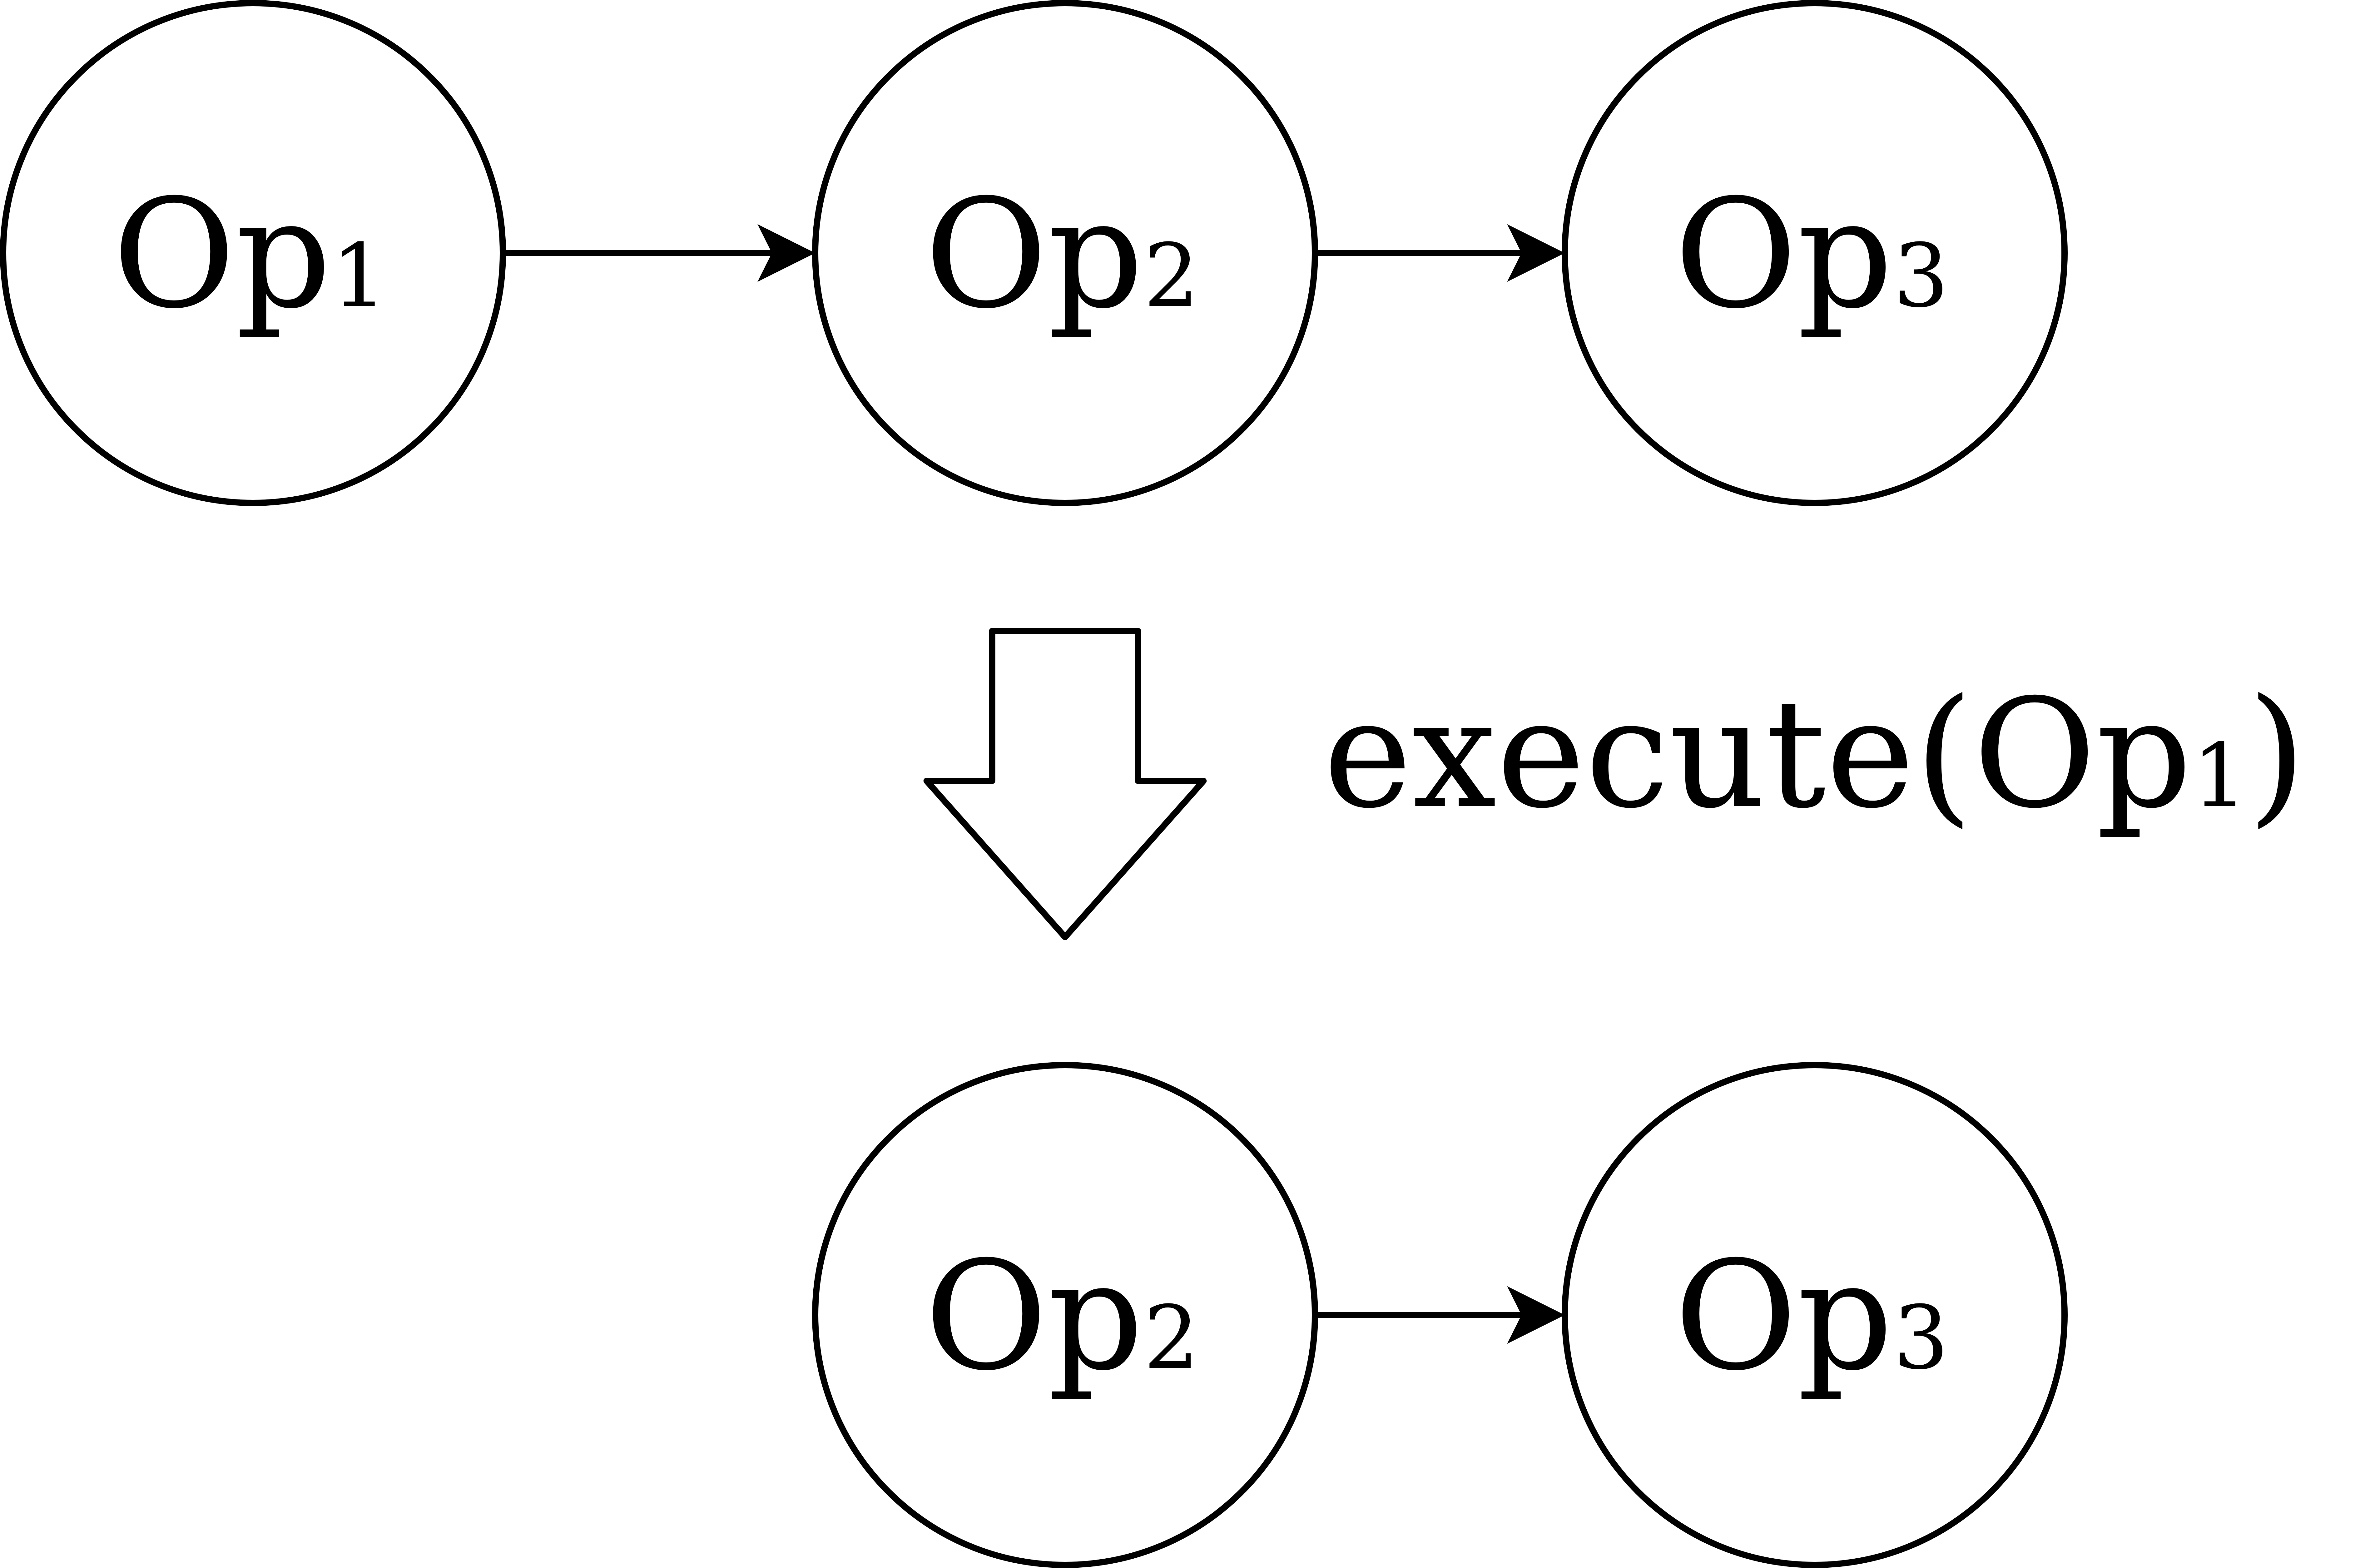
\includegraphics[width=\linewidth]{pics/casn-fail-remove.png}
          \captionof{figure}{\texttt{CAS-N} fails due to other process executing $Op_1$ in \texttt{v}}
          \label{casn-fail-remove-pic}
     \end{subfigure}
     \hfill
     \begin{subfigure}[b]{0.50\linewidth}
          \centering
          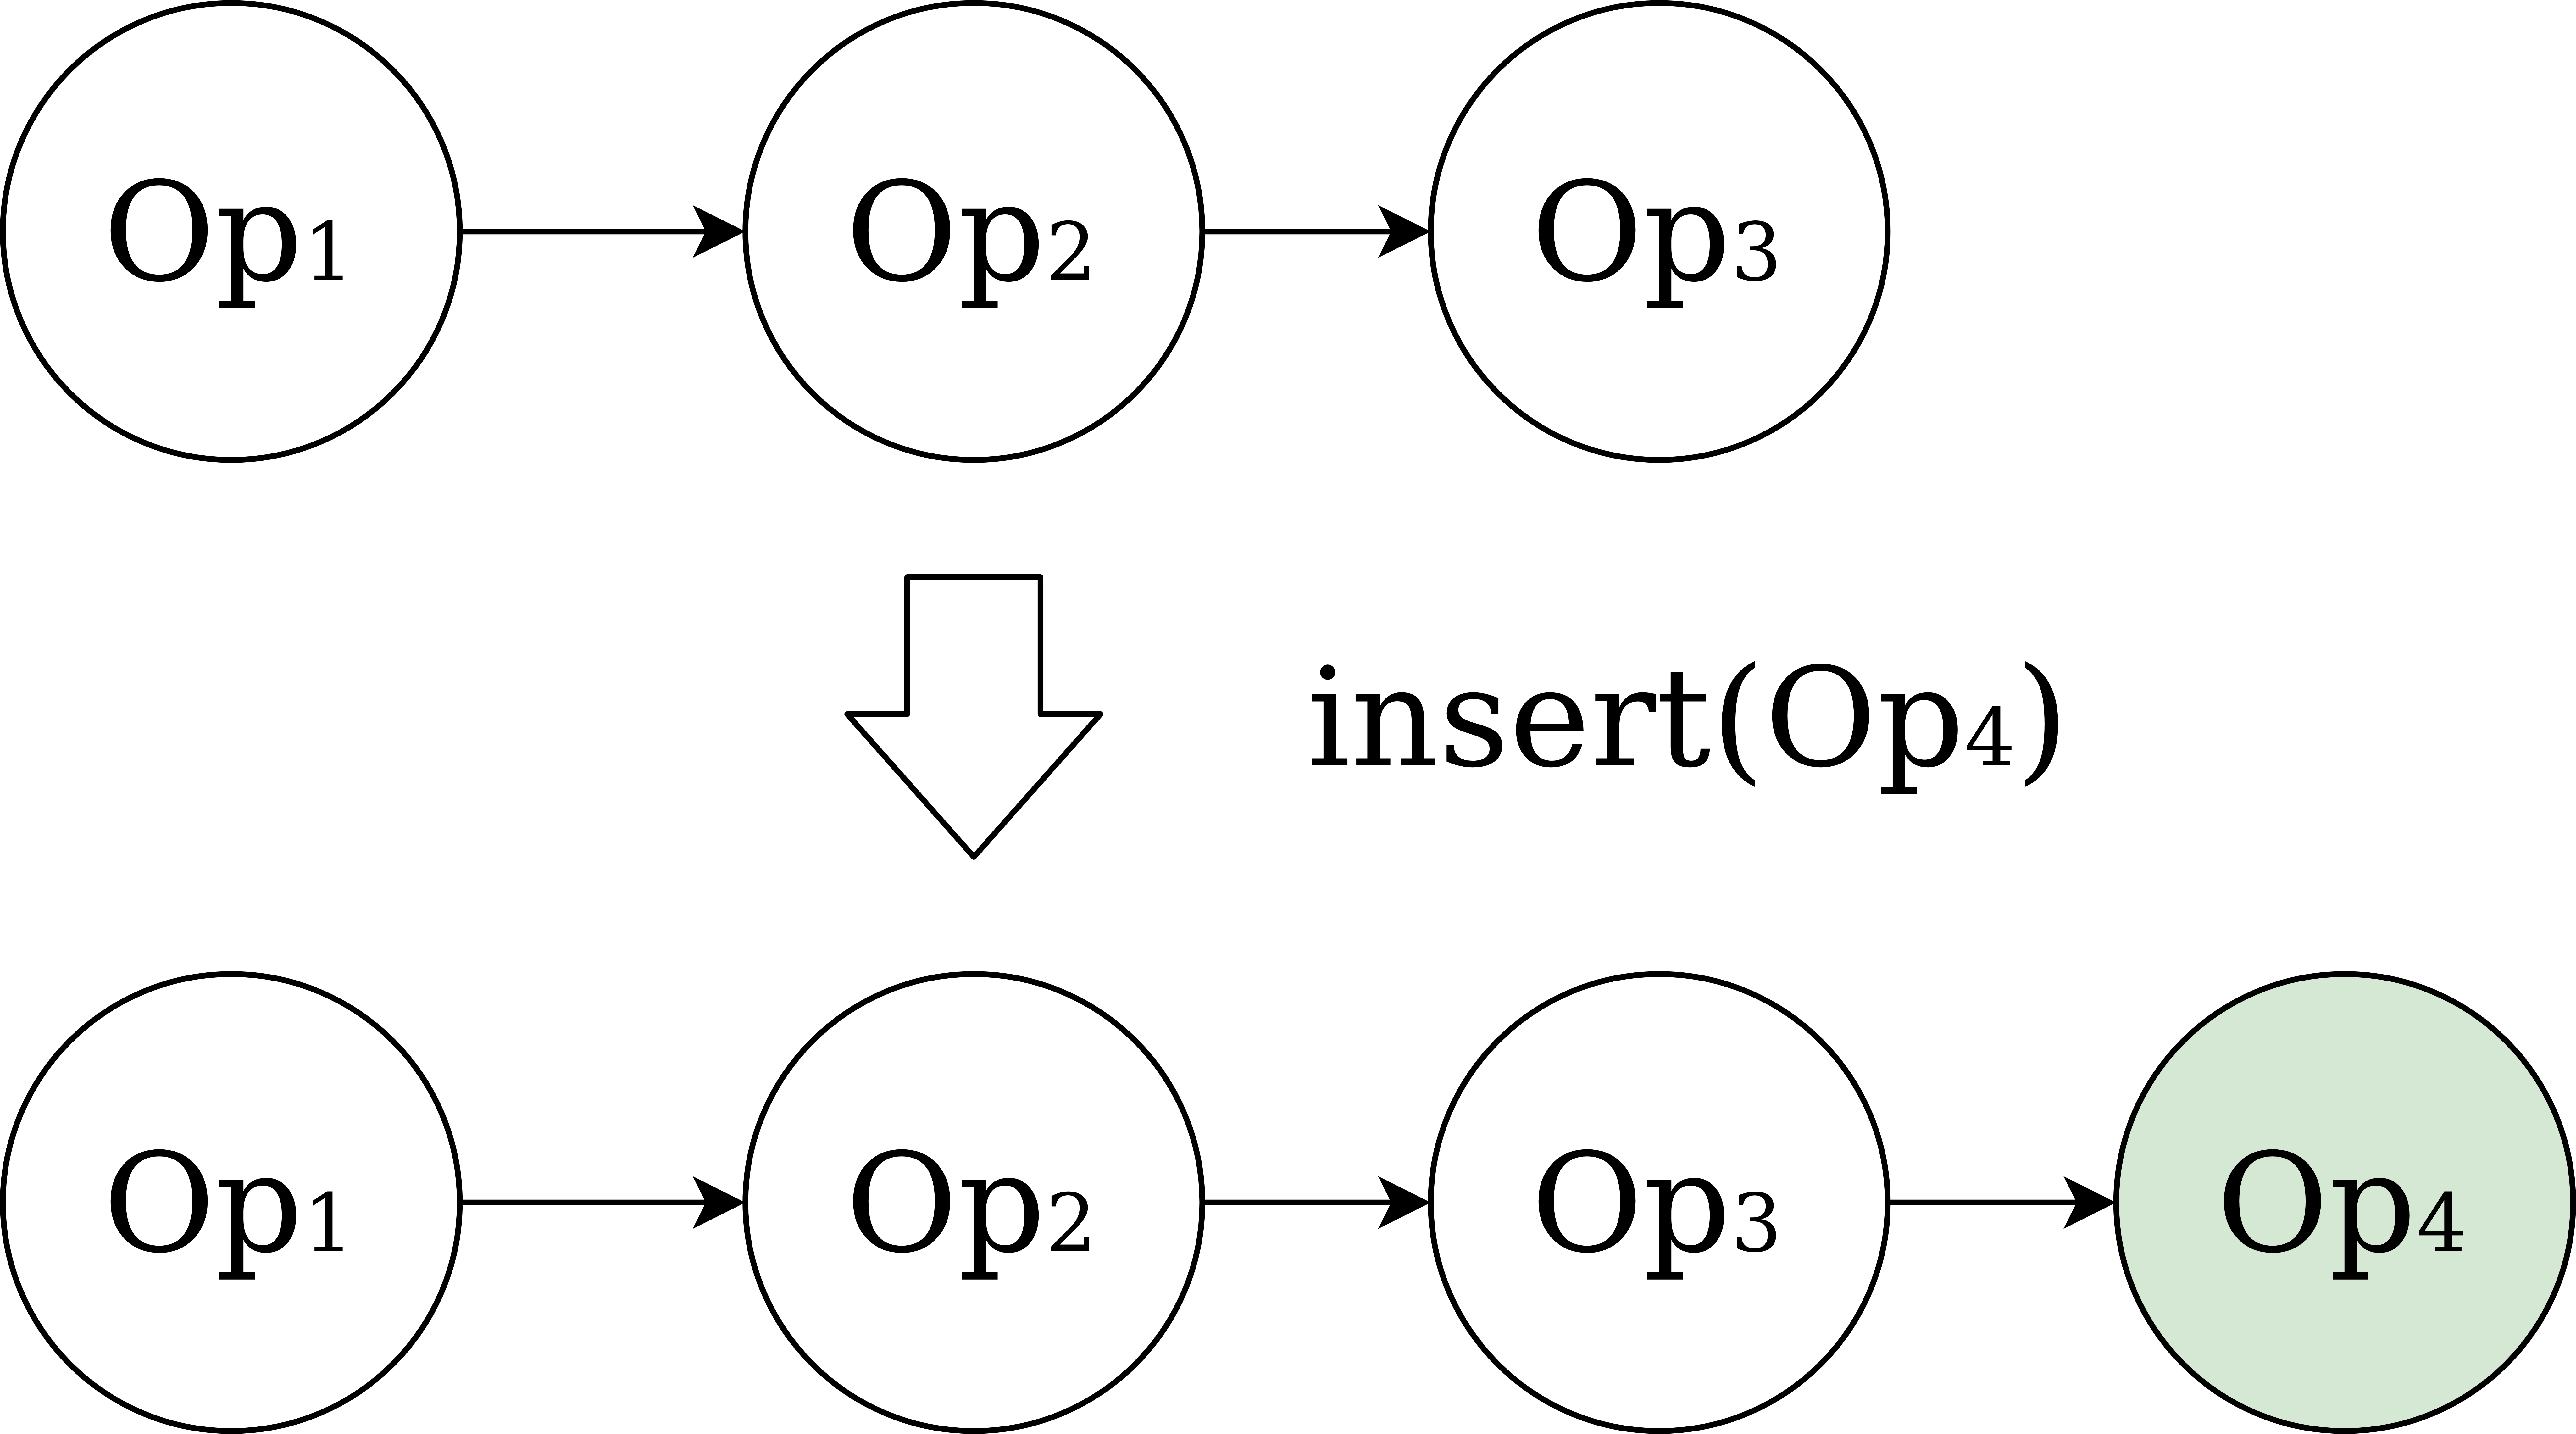
\includegraphics[width=\linewidth]{pics/casn-fail-insert.png}
          \captionof{figure}{\texttt{CAS-N} fails due to other process inserting new descriptor into \texttt{v} queue}
          \label{casn-fail-insert-pic}
     \end{subfigure}
    \caption{Reasons for \texttt{CAS-N} to return \texttt{false}}
    \label{casn-fail-pic}
\end{figure}

We can distinguish between these two situations by peeking descriptor from the head of \texttt{v} queue. If that descriptor still denotes the operation, we are trying to execute~--- we conclude, that situation (2) happened and try to execute that operation in \texttt{v} one more time. Otherwise, we can conclude, that some other process executed the operation, we are trying to execute, in node \texttt{v}, i.e., situation (1) happened. In that case, we may proceed to execute the next operation from \texttt{v} queue or to traverse the tree, depending on whether our initiated operation has been executed in \texttt{v} or not (see Section~\ref{operation-execution-chapter} for details).

Thus, the algorithm executing operation \texttt{op} in node \texttt{v} using \texttt{CAS-N} can be implemented the following way (Listing~\ref{op-process-node-casn-listing}):

\renewcommand{\lstlistingname}{Listing}
\begin{lstlisting}[caption={Algorithm for executing operation \texttt{op} in node \texttt{v} using \texttt{CAS-N}},label={op-process-node-casn-listing},escapeinside={(*}{*)}, captionpos=b]
fun execute_in_node(op, v):
    while true:
        cur_v_queue := v.Queue_Ptr
        if cur_v_queue.peek() (*$\neq$*) op:
            /* another process has executed op in v */
            return
        new_v_queue := cur_v_queue.pop_persistent()
        
        cas_registers := [&v.Queue_Ptr]
        cas_expected_values := [cur_v_queue]
        cas_new_values := [new_v_queue]
    
        C (*$\leftarrow$*) /* 
            set of v children in which the execution of op should continue 
        */
        for c in C:
            cur_child_state := c.State_Ptr
            new_child_state := op.get_modified_state(cur_child_state)
            cas_registers.append(&c.State_Ptr)
            cas_expected_values.append(cur_child_state)
            cas_new_values.append(new_child_state)
        
            cur_child_queue = c.Queue_Ptr
            new_child_queue := cur_child_queue.push_persistent(op)
            cas_registers.append(&c.Queue_Ptr)
            cas_expected_values.append(cur_child_queue)
            cas_new_values.append(new_child_queue)
        
        cas_res := multi_cas(
            n = cas_registers.length(), 
            Registers = cas_registers,
            expected_values = cas_expected_values, 
            new_values = cas_new_values
        )
        if cas_res:
            return
        /* 
        Otherwise, try to execute op in v 
        from the very beginning one more time 
        */
\end{lstlisting}

The algorithm is lock-free since each retry means that some other descriptor was inserted into \texttt{v} queue, i.e., another process executed some operation in \texttt{v} parent.

\section{Execution of an operation in a node without \texttt{CAS-N}}
\label{no-casn-chapter}

Despite the fact that \texttt{CAS-N} provides the ability to execute an operation in a node atomically with lock-freedom progress guarantees, this concurrent primitive remains very inefficient due to indirections and a dynamic memory allocation. Thus, we want to design a method to execute operations in a node without using \texttt{CAS-N}.

The algorithm to execute operation \texttt{Op} in node \texttt{v} consists of the following steps:

\begin{nenum}
    \item Determine the set of children \texttt{C}, in which execution of \texttt{Op} should continue.
    
    \item Traverse the set \texttt{C}. For each child \texttt{c} from \texttt{C}:
        \begin{nenum}
            \item Atomically read \texttt{c} state.
            
            \item If \texttt{c} state has not been modified by \texttt{Op} yet, modify it. We explain how to do it below.
            
            \item Insert \texttt{Op} descriptor to \texttt{c} queue if it has not been yet inserted. We explain in Section~\ref{push-if-section} how to do it.
        \end{nenum}
    
    \item If \texttt{Op} descriptor has not been yet removed from \texttt{v} queue, remove it. We explain in Section~\ref{pop-if-section} how to do it.
\end{nenum}

\bigbreak

Note, that the removal of \texttt{Op} descriptor from the head of \texttt{v} queue should be done after the insertion of \texttt{Op} descriptor to child queues and modification of child states are finished. Otherwise, the execution of later operations in \texttt{v} may start before the execution of \texttt{Op} in \texttt{v} is finished, which may break the main invariant (Section~\ref{main-invariant-chapter}). Consider, for example, the following scenario:

\begin{nenum}
    \item Descriptors of $O_1$ and $O_2$ are located in \texttt{v} queue and execution of both $O_1$ and $O_2$ should be continued in \texttt{v.Right} (Fig.~\ref{remove-last-1}).
    
    \item Process \texttt{P} reads $O_1$ descriptor from the head of \texttt{v} queue and starts executing $O_1$ in \texttt{v}: removes $O_1$ descriptor from the head of \texttt{v} queue before inserting it to \texttt{v.Right} queue (Fig.~\ref{remove-last-2}).
    
    \item \texttt{P} is suspended by the OS.
    
    \item Process \texttt{R} reads $O_2$ descriptor from the head of \texttt{v} queue and executes $O_2$ in \texttt{v}: removes it from the head of \texttt{v} queue and inserts it to \texttt{v.Right} queue (Fig.~\ref{remove-last-3}). 
    
    \item Process \texttt{P} finishes executing $O_1$ in \texttt{v}: inserts $O_1$ descriptor to \texttt{v.Right} queue (Fig.~\ref{remove-last-4}). Thus, the descriptors are placed in \texttt{v.Right} queue in the wrong order and the main invariant is broken: $O_2$ will be applied to \texttt{v.Right} subtree before $O_1$, despite $O_1$ descriptor was inserted to \texttt{v} queue before $O_2$ descriptor.
\end{nenum}

\begin{figure}[H]
     \centering
     \begin{subfigure}[b]{0.45\linewidth}
          \centering
          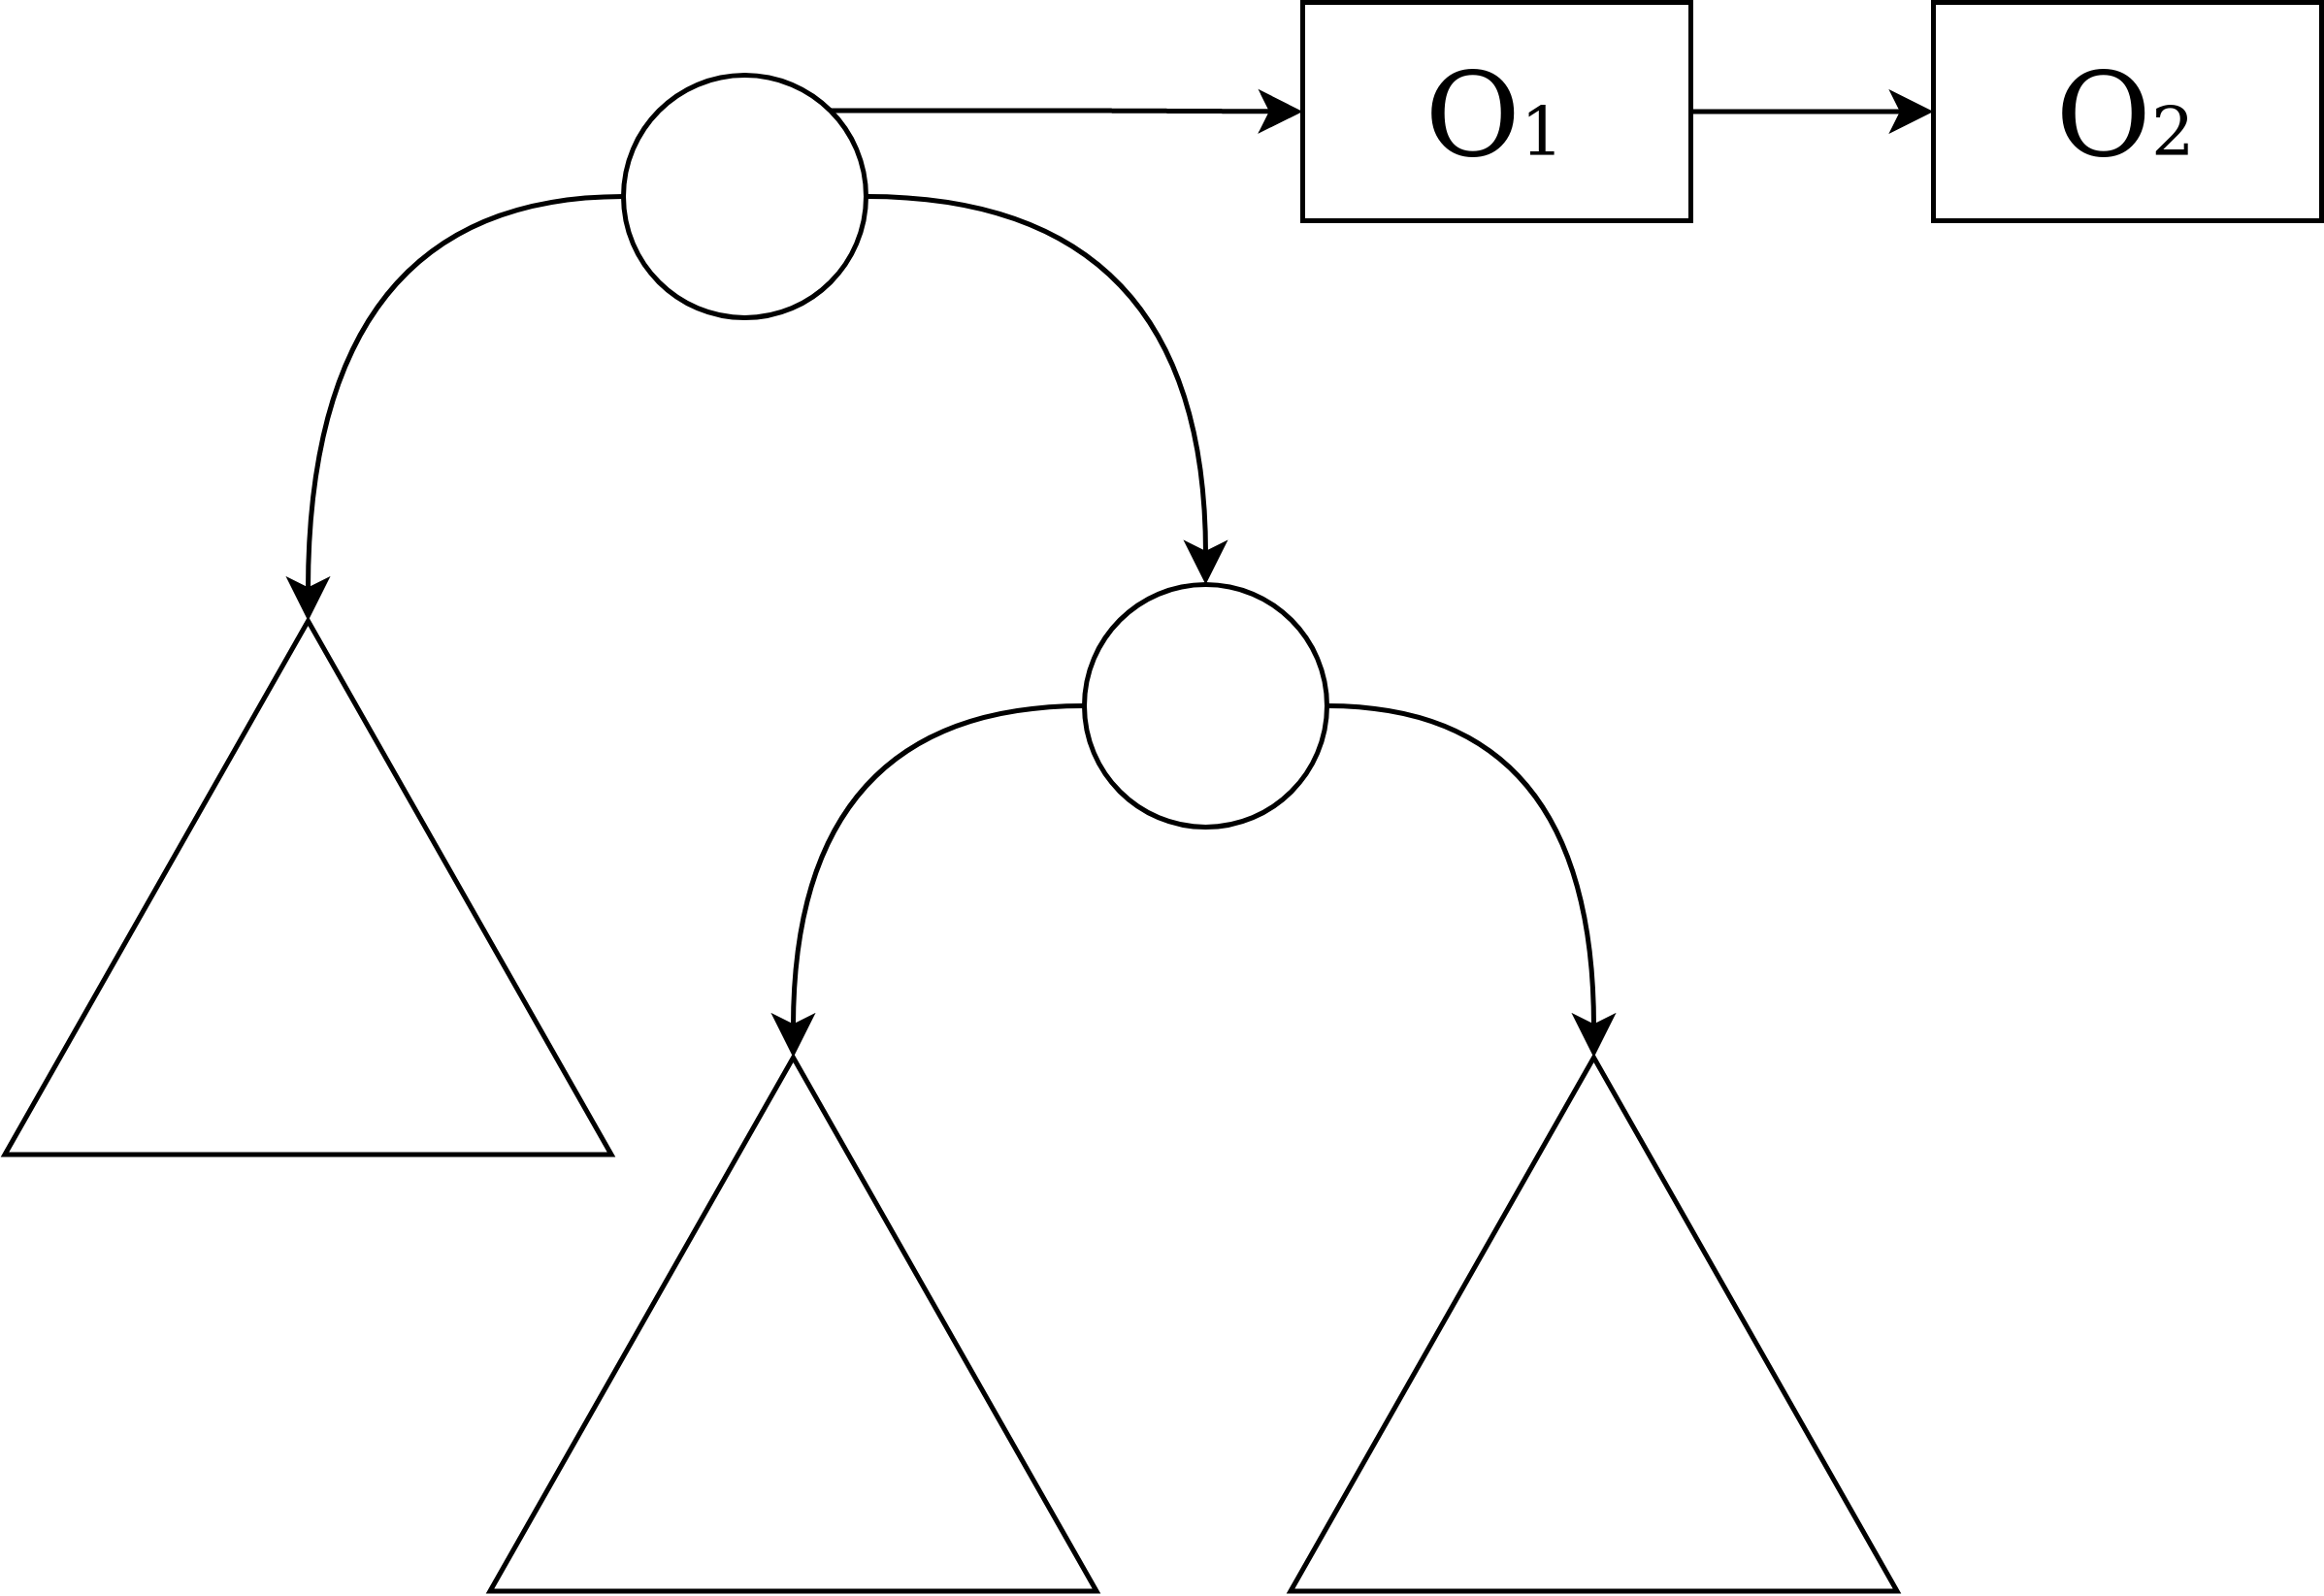
\includegraphics[width=\linewidth]{pics/remove-last-1.png}
          \captionof{figure}{The initial tree structure}
          \label{remove-last-1}
     \end{subfigure}
     \hfill
     \begin{subfigure}[b]{0.45\linewidth}
          \centering
          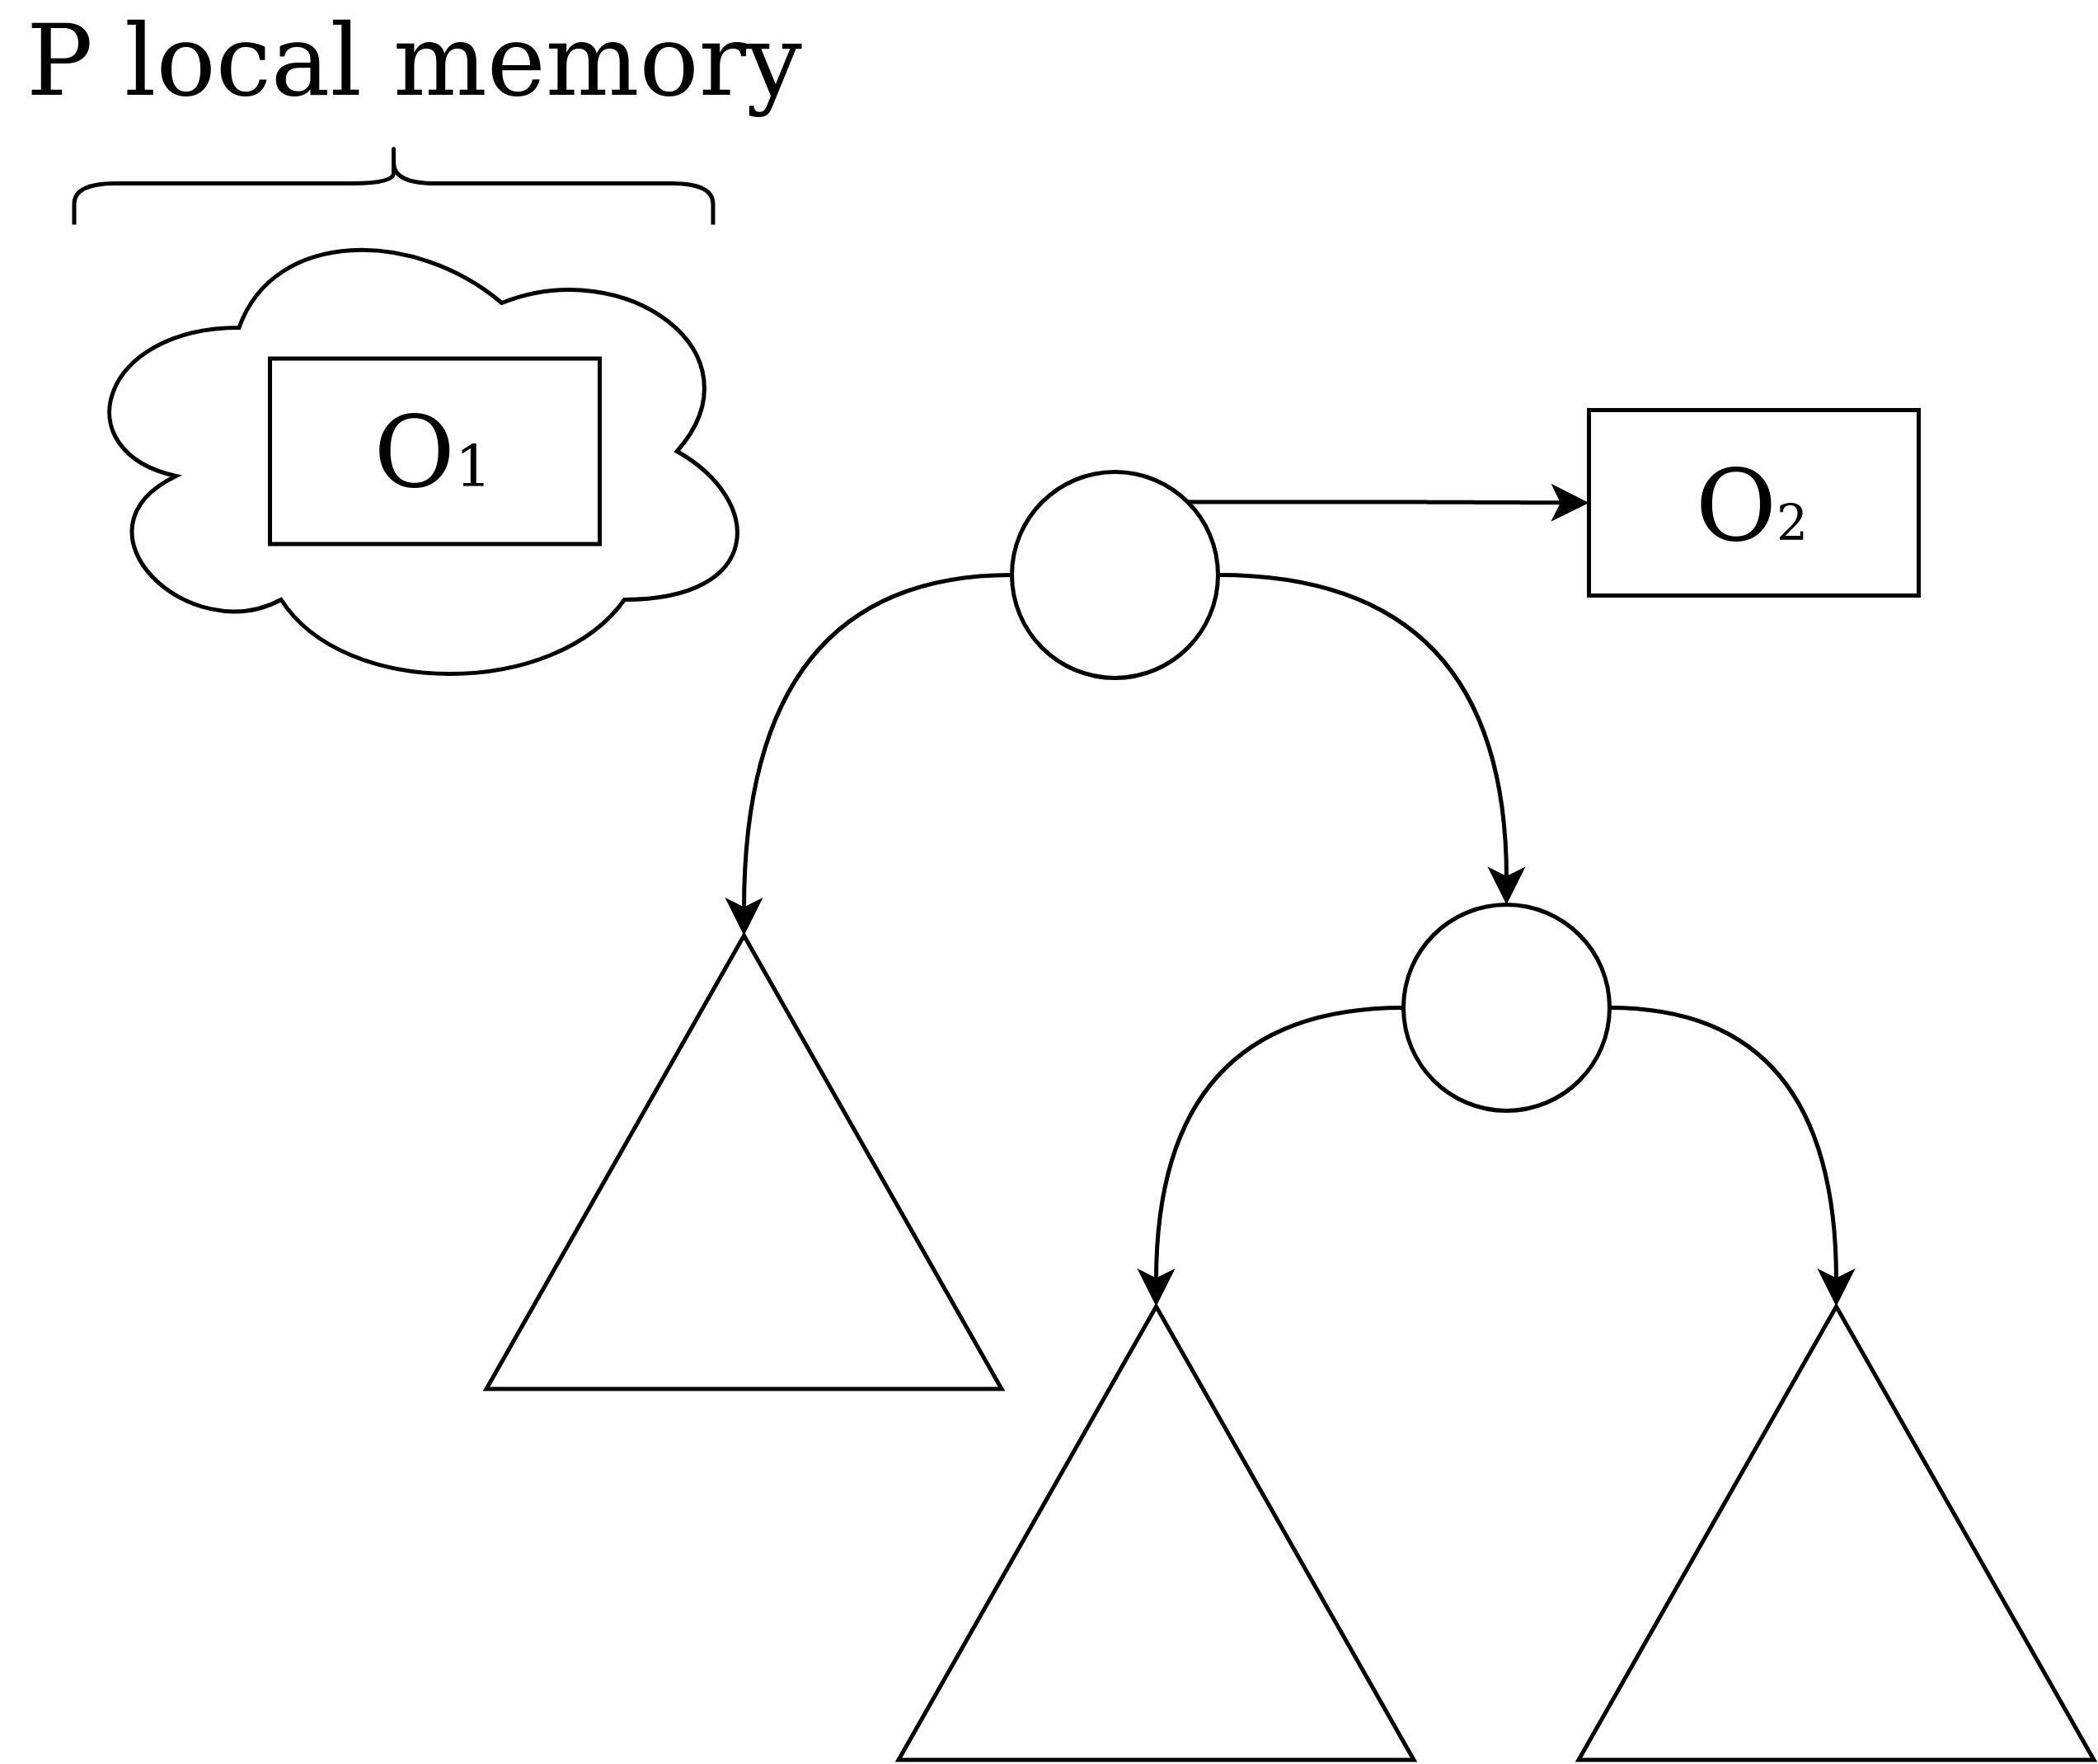
\includegraphics[width=\linewidth]{pics/remove-last-2.png}
          \captionof{figure}{Process \texttt{P} removes $O_1$ descriptor from the head of the parent queue before inserting it to the child queue}
          \label{remove-last-2}
     \end{subfigure}
     \hfill
     \begin{subfigure}[b]{0.45\linewidth}
          \centering
          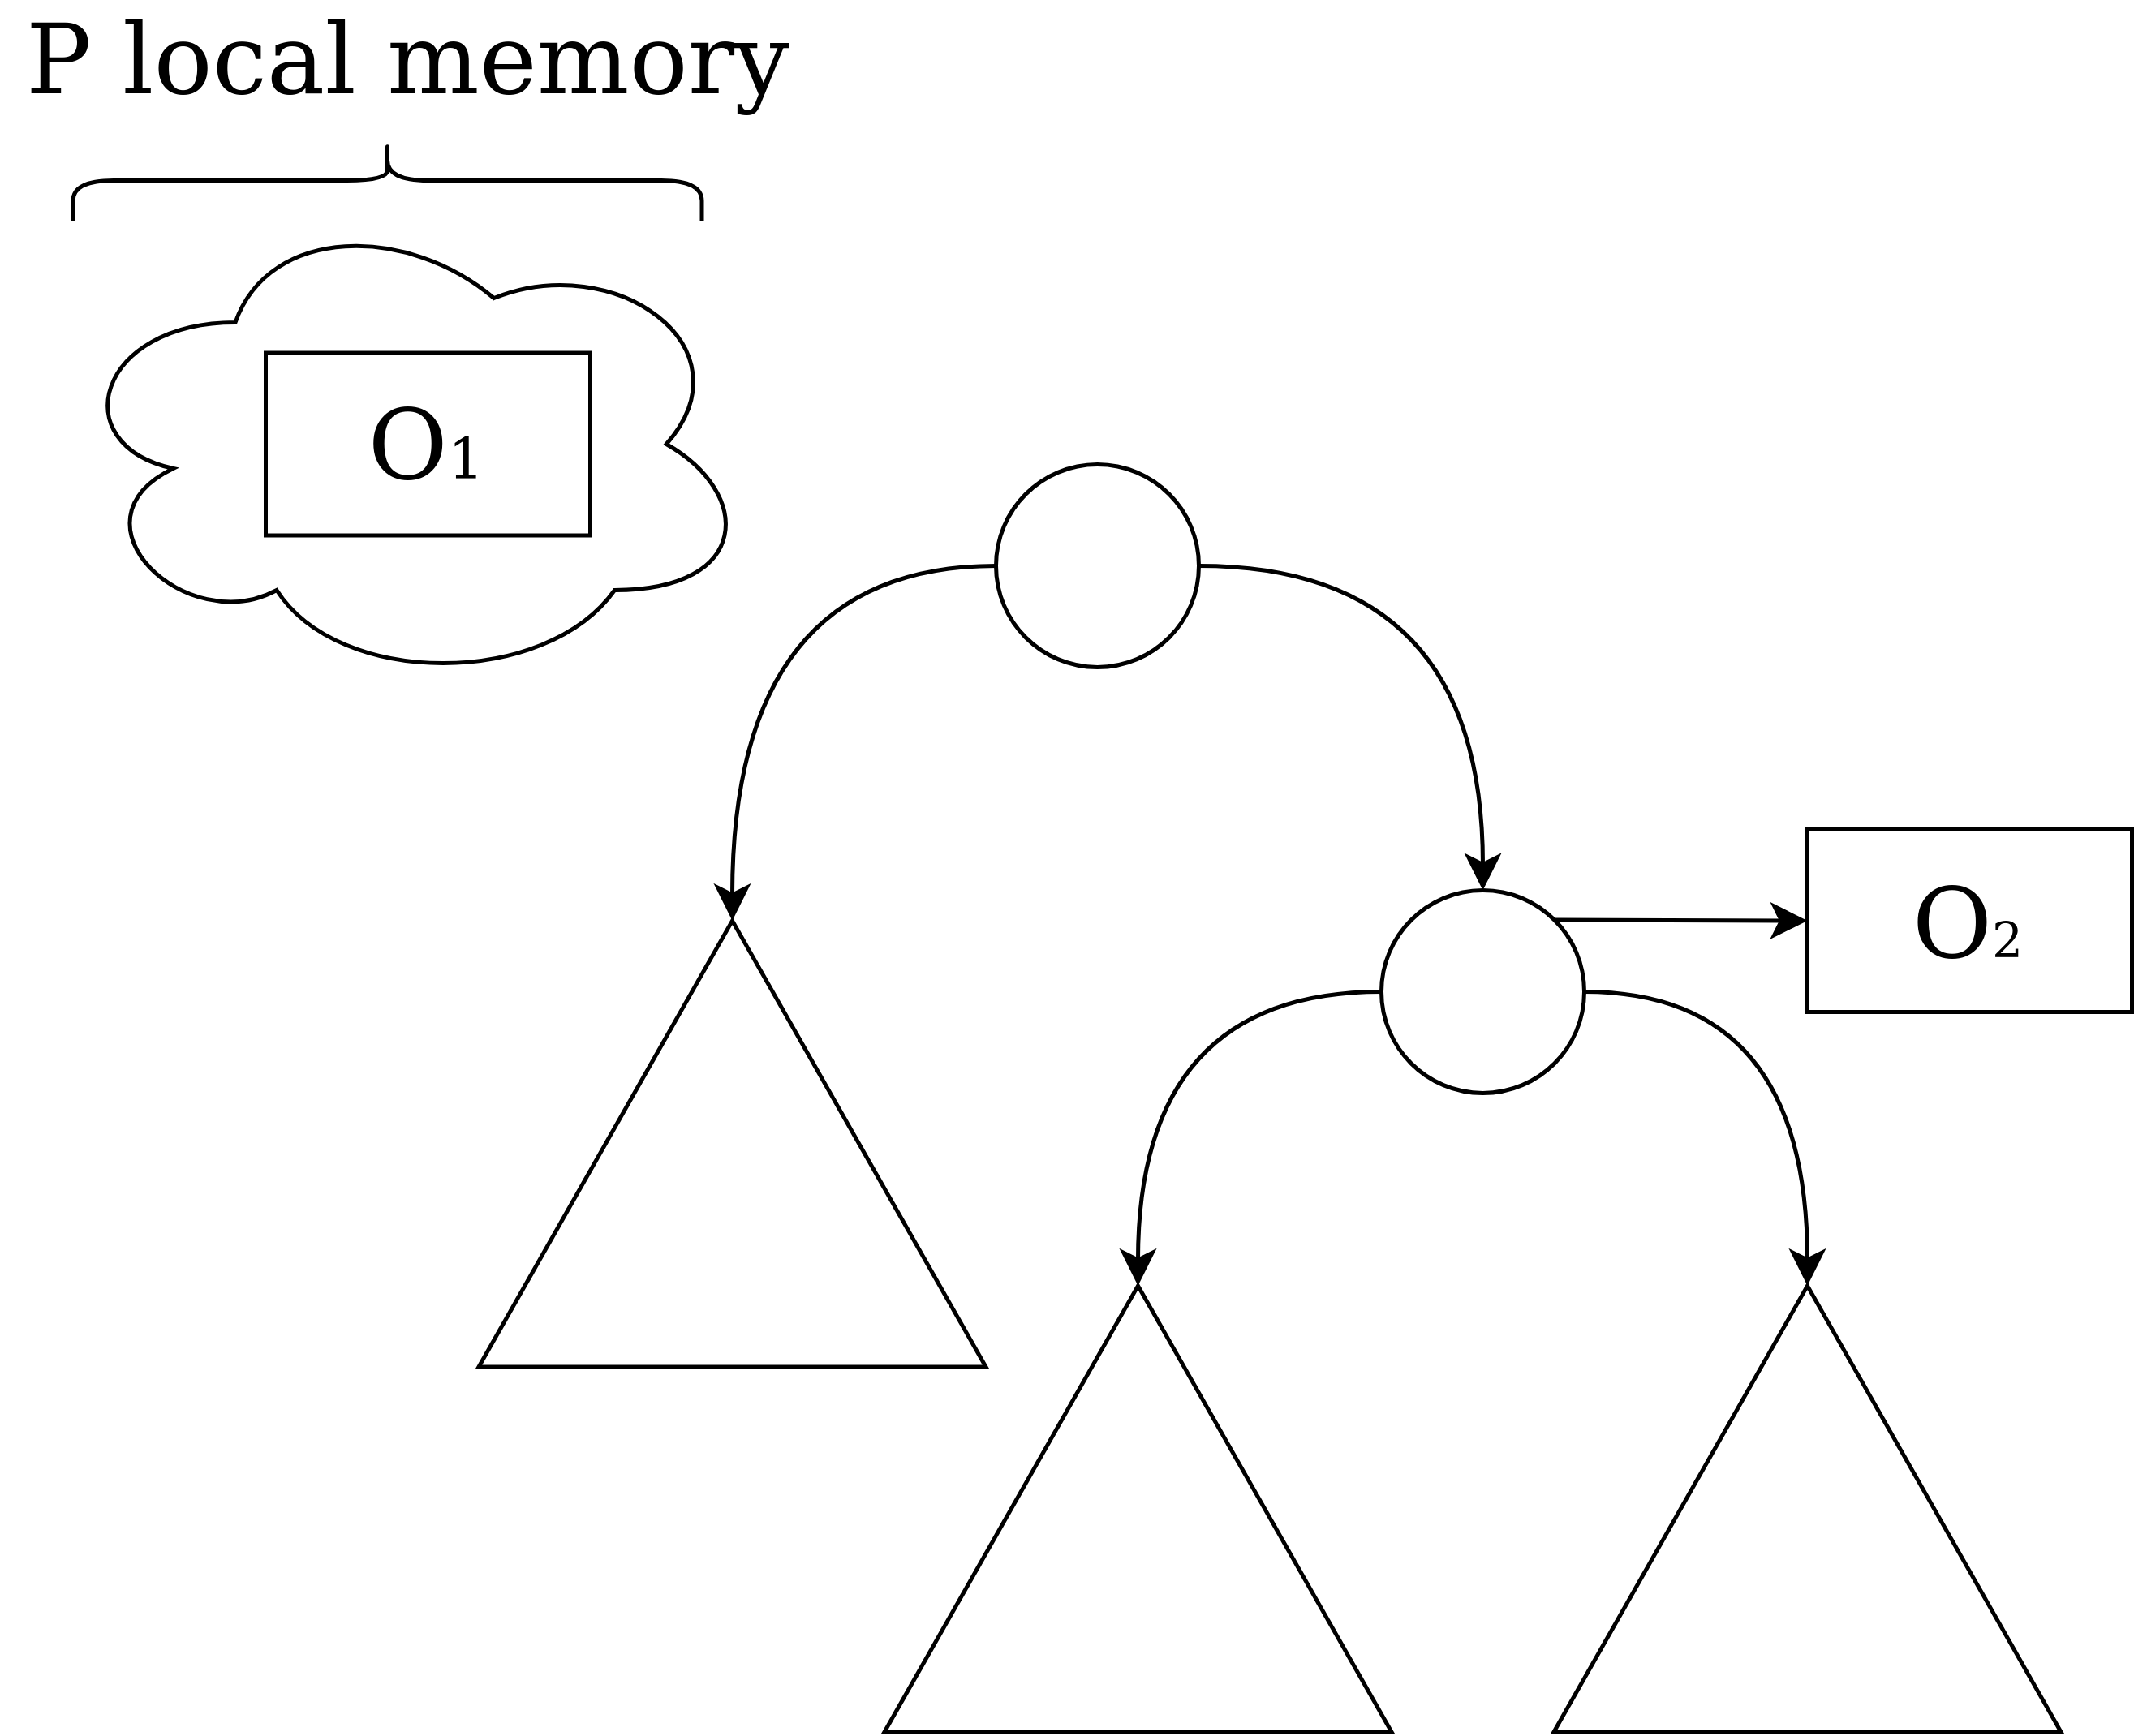
\includegraphics[width=\linewidth]{pics/remove-last-3.png}
          \captionof{figure}{Process \texttt{R} executes $O_2$ in \texttt{v}}
          \label{remove-last-3}
     \end{subfigure}
     \hfill
     \begin{subfigure}[b]{0.45\linewidth}
          \centering
          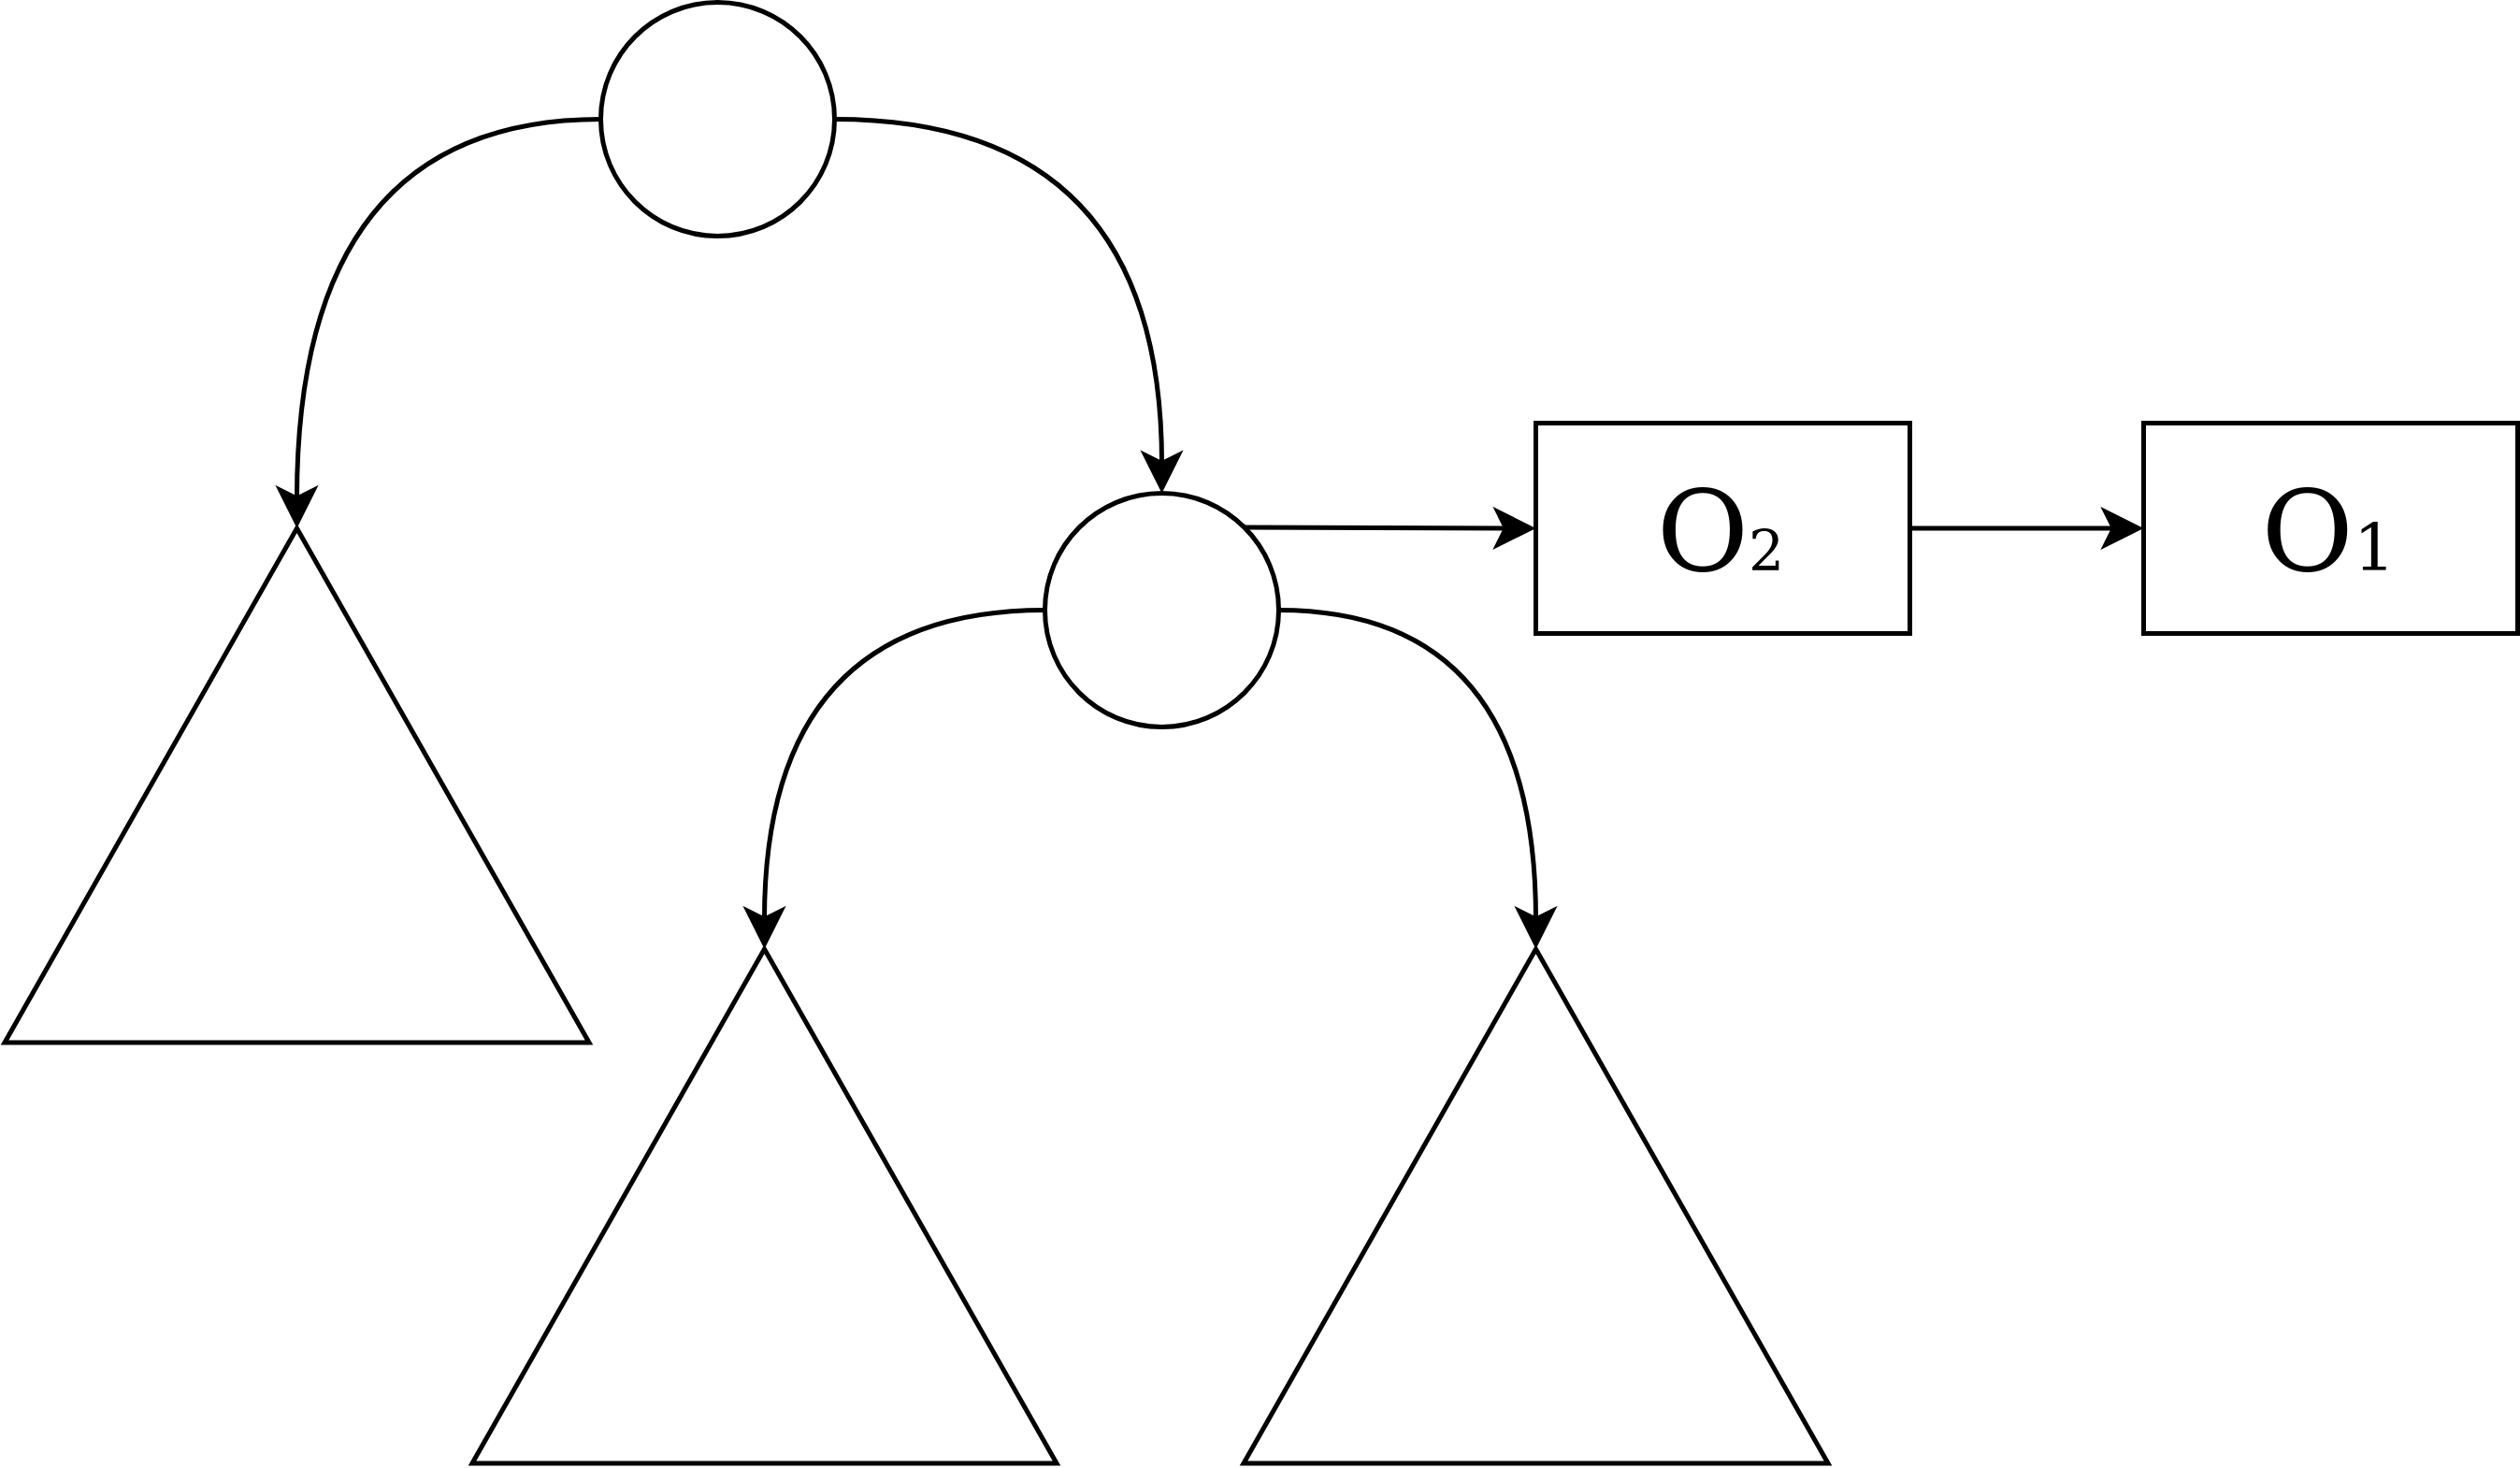
\includegraphics[width=\linewidth]{pics/remove-last-4.png}
          \captionof{figure}{Process \texttt{P} finishes executing $O_1$ in node \texttt{v}}
          \label{remove-last-4}
     \end{subfigure}
    \caption{The main invariant is broken if a descriptor is removed from the head of the parent queue before being inserted to child queues}
    \label{remove-last-pic}
\end{figure}
 
\bigbreak

Note also, that actions (2) and (3) may be executed by multiple processes concurrently. Consider the following scenario:

\begin{nenum}
    \item Descriptor of operation \texttt{Op} is located at the head of \texttt{v} queue, execution of \texttt{Op} should continue at \texttt{v.Left};
    
    \item Processes \texttt{P} and \texttt{Q} both read \texttt{Op} descriptor from the head of \texttt{v} queue;
    
    \item \texttt{P} and \texttt{Q} both try to modify \texttt{v.Left} state;
    
    \item \texttt{P} and \texttt{Q} both try to push \texttt{Op} descriptor to \texttt{v.Left} queue;
    
    \item \texttt{P} and \texttt{Q} both try to remove \texttt{Op} descriptor from the head of \texttt{v} queue;
\end{nenum}

\bigbreak

Thus, inserting the descriptor to child queues, modifying child states, and removing the descriptor from the parent queue should happen exactly once, no matter how many processes are working on the descriptor concurrently.

Exactly-once insertion to and removal from queues is handled by our implementation of concurrent queues. Queues provide two procedures:

\begin{itemize}
    \item \texttt{push\_if} inserts the descriptor to the tail of the queue only if it has not been inserted yet, otherwise, the queue is left unmodified. The implementation of this procedure is discussed in Section~\ref{push-if-section}.

    \item \texttt{pop\_if} removes the descriptor from the head of the queue only if it has not been removed yet, otherwise, the queue is left unmodified. The implementation of this procedure is discussed in Section~\ref{pop-if-section}.
\end{itemize}

\bigbreak

Therefore, in this chapter we explain on how to change the node state exactly once and how to read it atomically.

The main problem with reading the state atomically is that it may consist of multiple fields. To solve this problem, we do not store the state directly inside the node (Fig.~\ref{state-storing-inside-pic})~--- instead, the immutable state is located somewhere in the heap and the node will contain only one field \texttt{S\_Ptr}~--- the pointer to the heap location of the state (Fig.~\ref{state-storing-pic}).

\begin{figure}[H]
     \centering
     \begin{subfigure}[b]{0.45\linewidth}
          \centering
          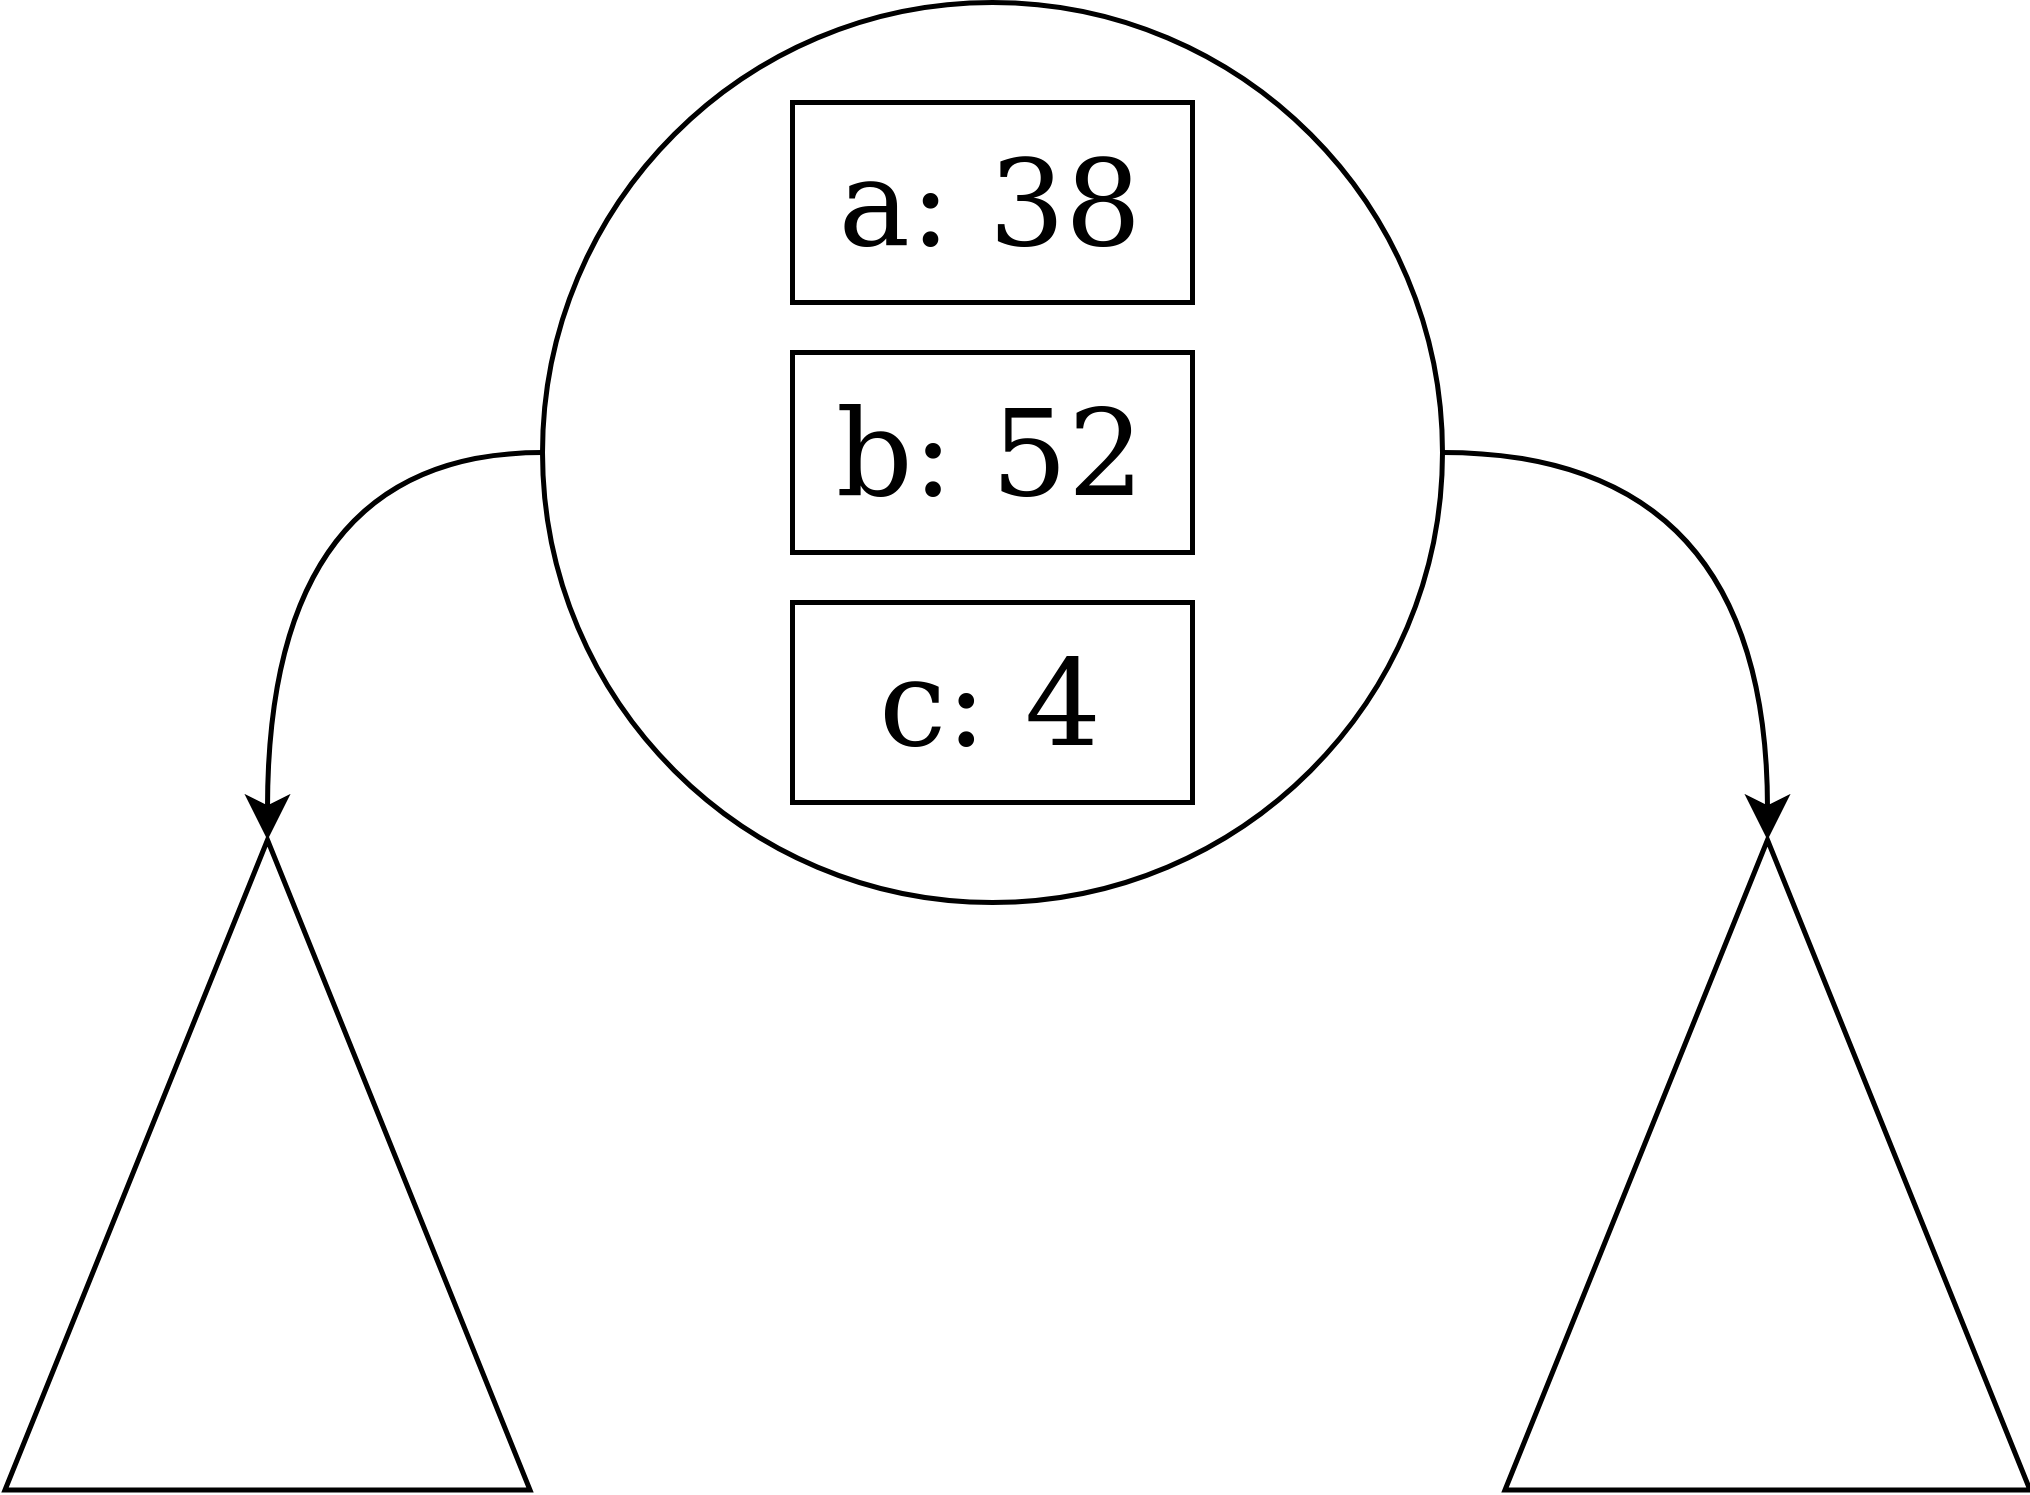
\includegraphics[width=\linewidth]{pics/state-storing-inside.png}
          \captionof{figure}{Storing node state inside the node}
          \label{state-storing-inside-pic}
     \end{subfigure}
     \hfill
     \begin{subfigure}[b]{0.45\linewidth}
          \centering
          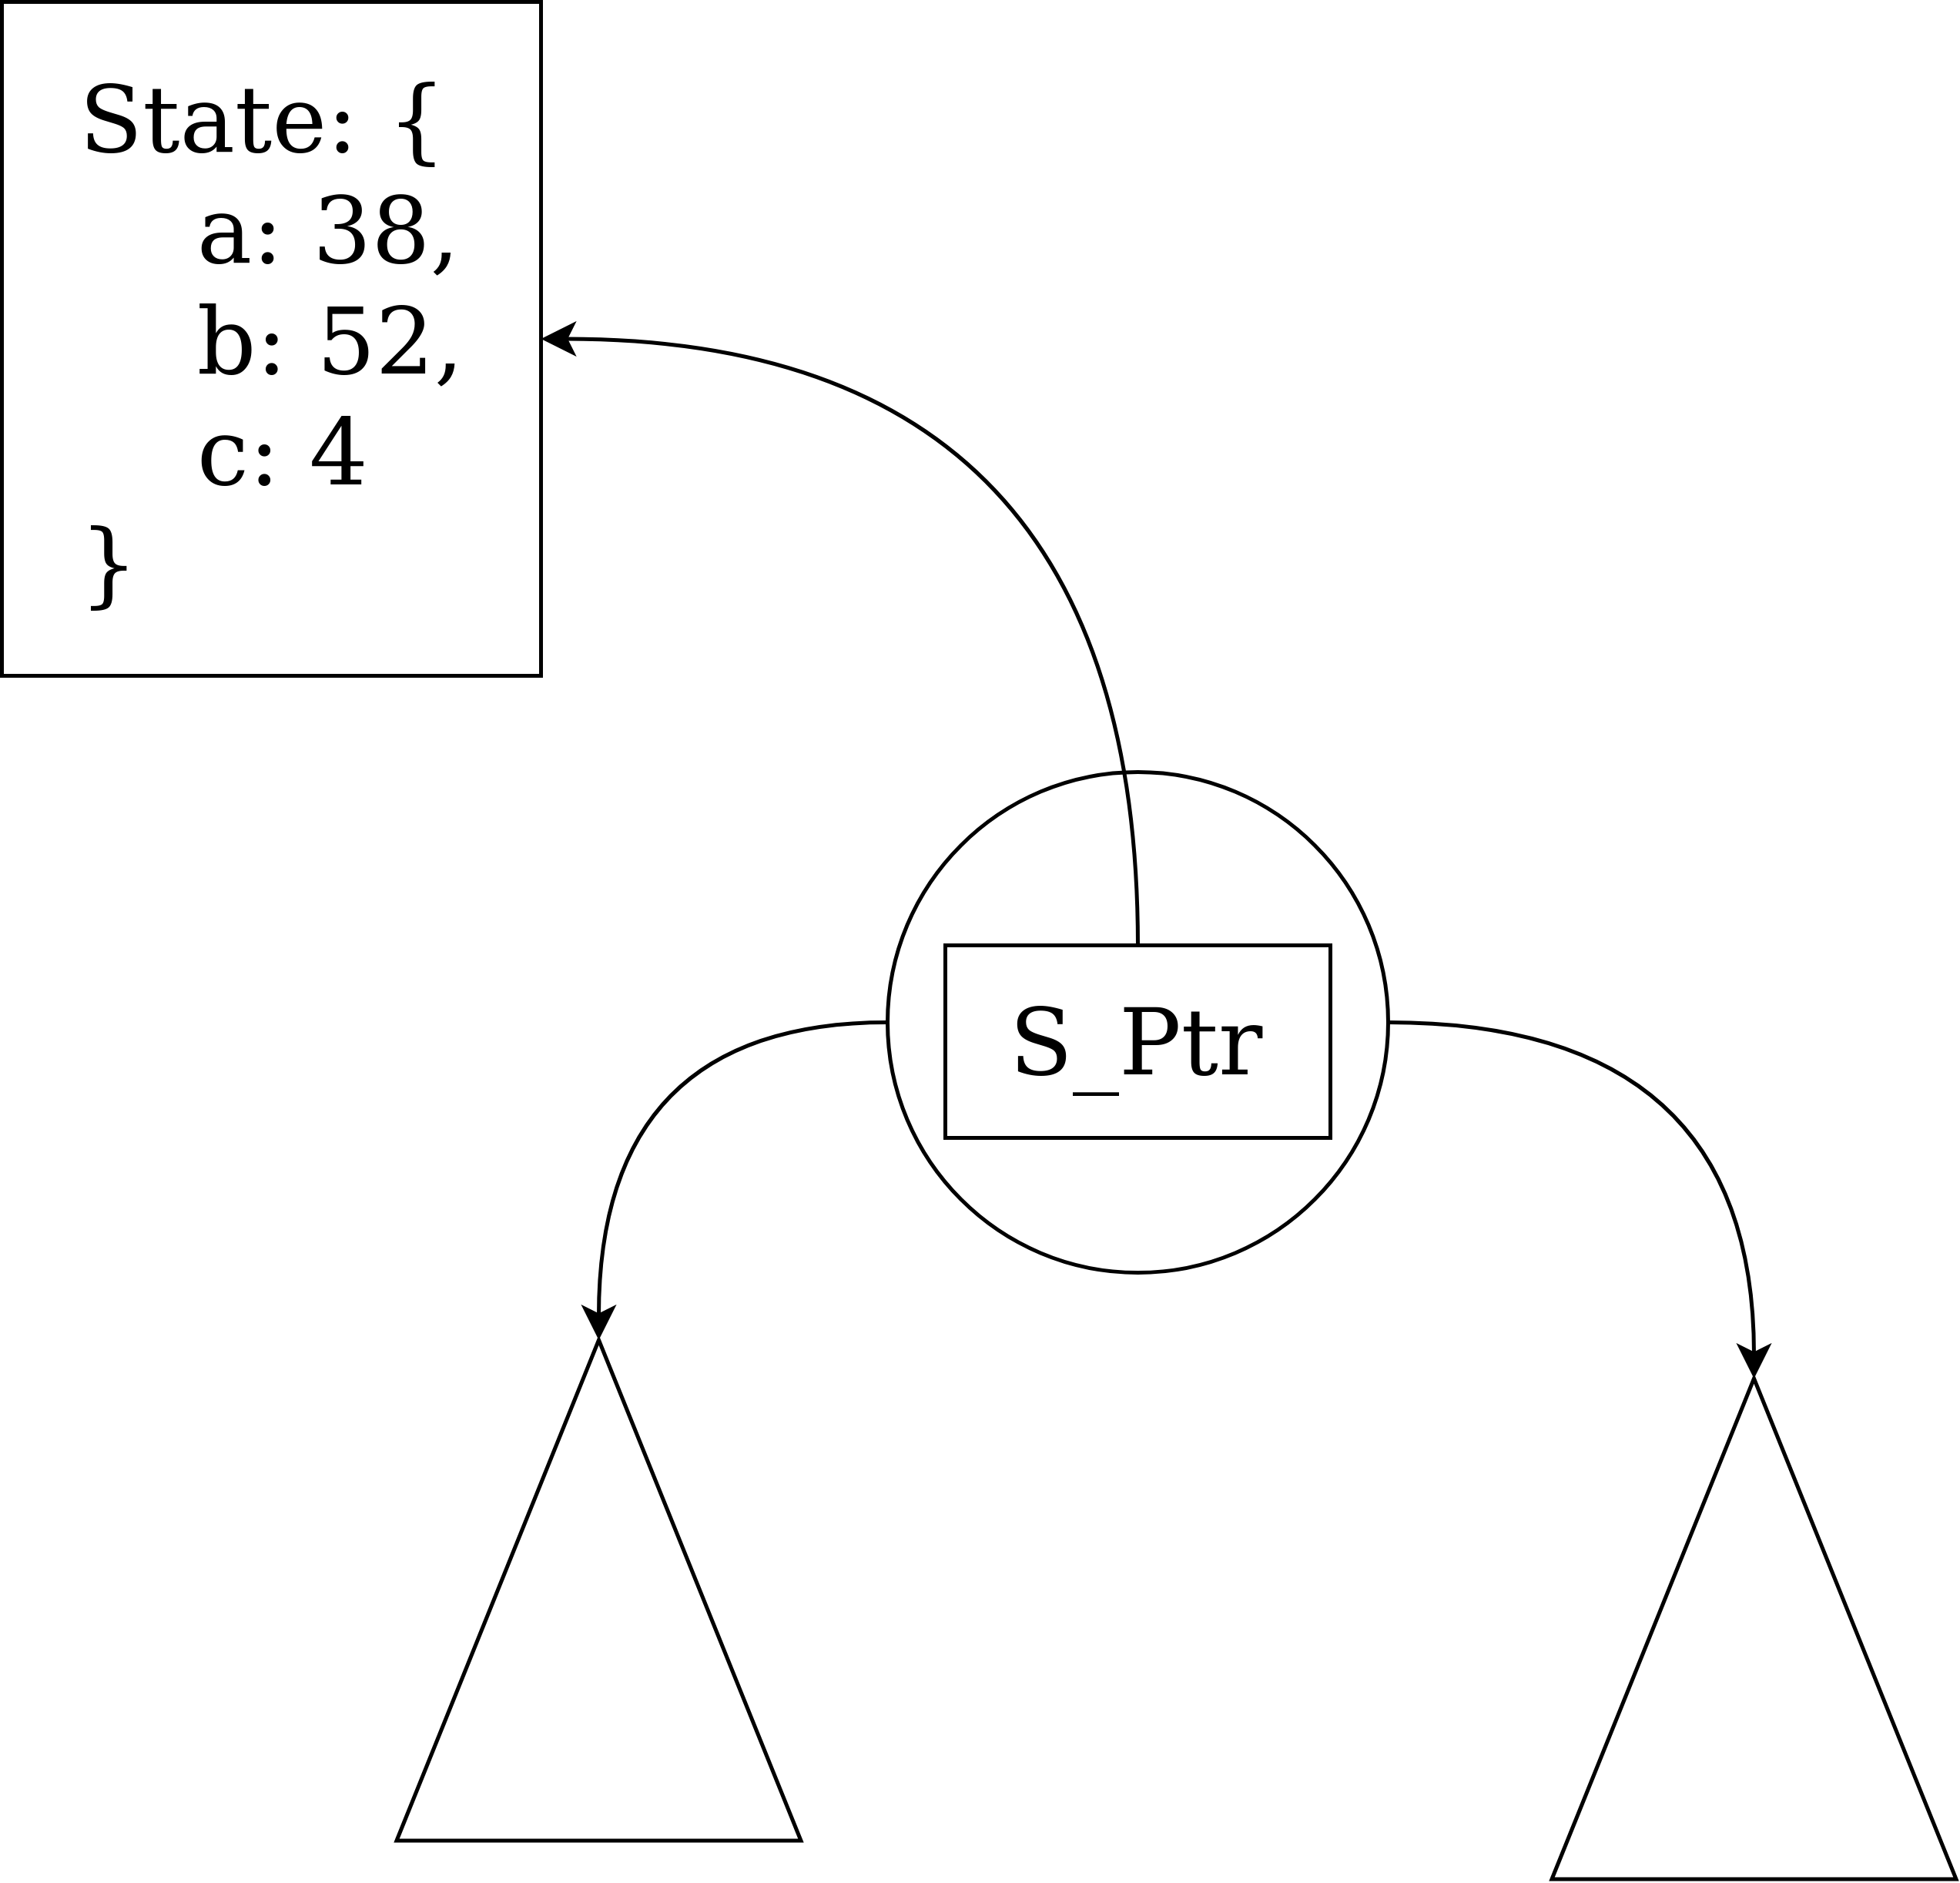
\includegraphics[width=\linewidth]{pics/state-storing.png}
          \captionof{figure}{Storing node state in a separate memory location, while storing the pointer to it inside the node}
          \label{state-storing-pic}
     \end{subfigure}
    \caption{Different methods of storing the node state}
    \label{remove-last-pic}
\end{figure}

The state, located in the heap, is considered immutable and is never modified. To modify the node state, we simply do the following (Fig.~\ref{state-change-pic}):

\begin{nenum}
    \item Create the structure, corresponding to the modified state, with an arbitrary set of fields changed.
    \item Place the modified state somewhere in the heap.
    \item Change the \texttt{node.S\_Ptr} so than it points to the modified state.
\end{nenum}

\begin{figure}[H]
  \centering
  \caption{The modification of the node state via the creation of a new state structure and change of \texttt{S\_Ptr}}
  \label{state-change-pic}
  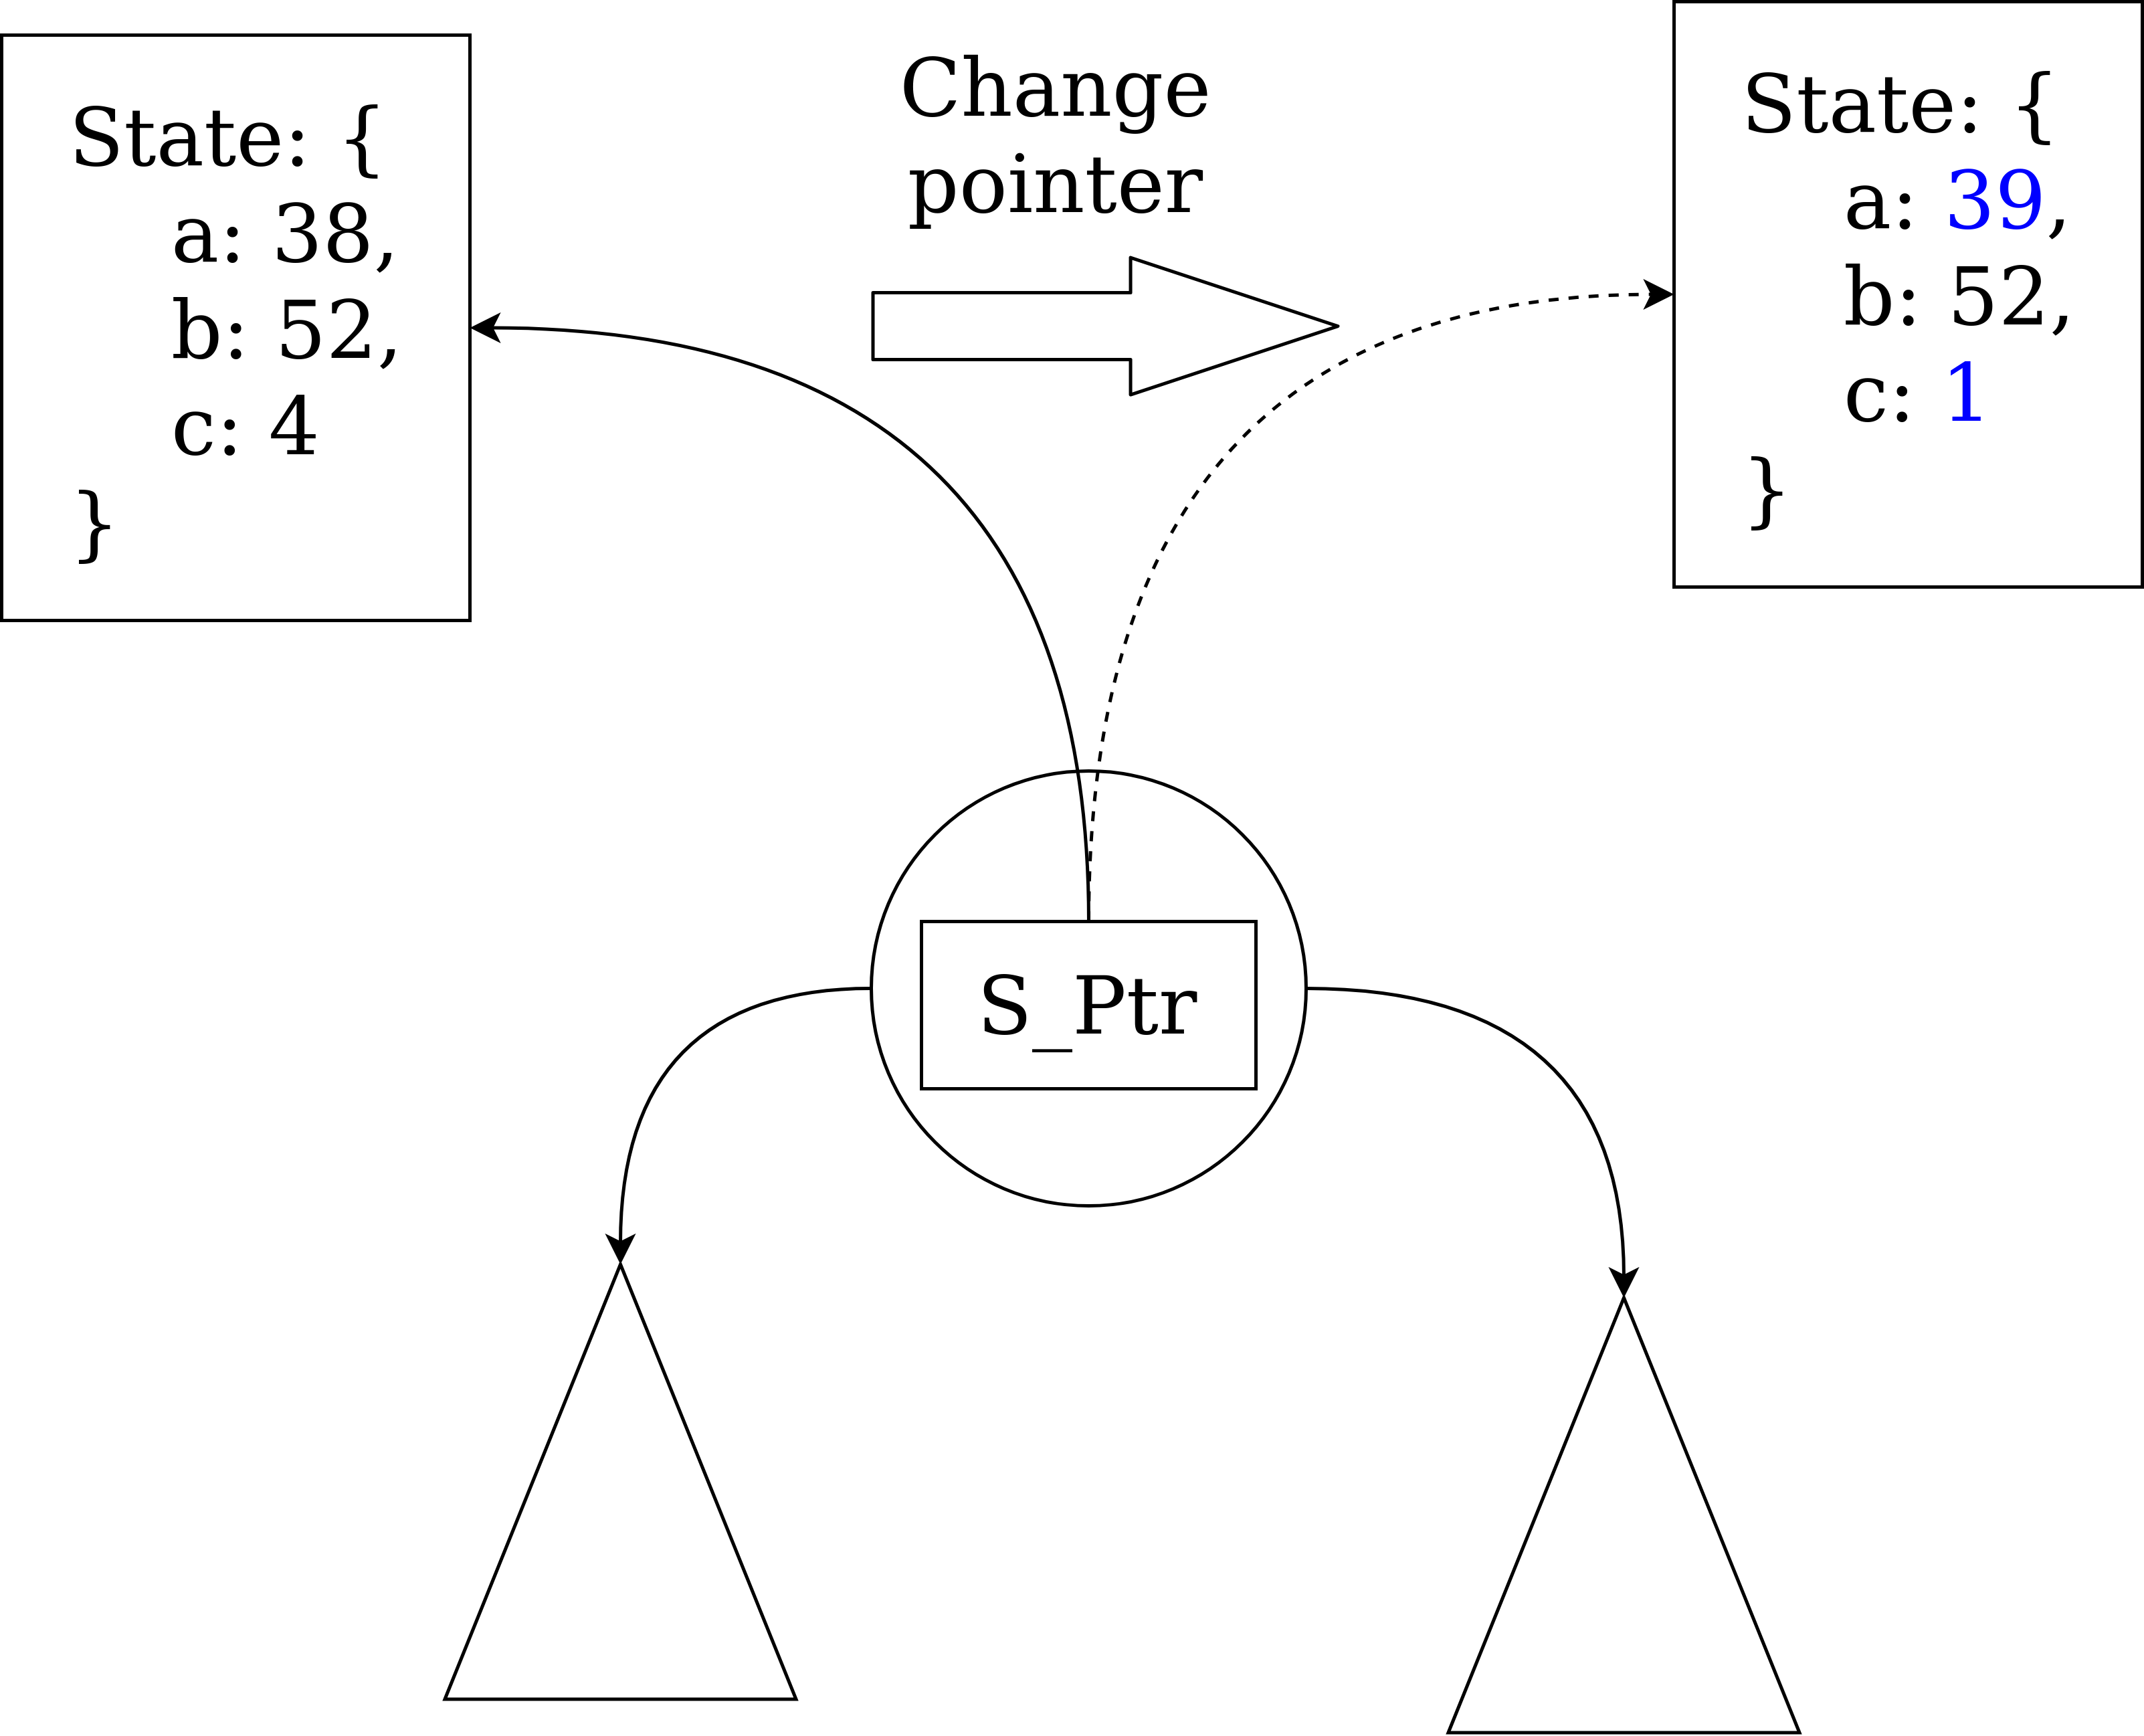
\includegraphics[width=0.7\linewidth]{pics/state-change.png}
\end{figure}

To read the state atomically, we simply read the \texttt{S\_Ptr} register. After that, we can safely access any field from the state structure, pointed at by the fetched pointer, without worrying that the state structure is being modified concurrently by another process. Since the structure is immutable, it can never be modified by another process.

Now, we return to the problem of modifying the state exactly once. In the state we shall store one additional field: \texttt{Ts\_Mod}~--- timestamp of the operation, that was the last to modify the state. Thus, if the operation \texttt{Op} is willing to modify node \texttt{v} state, we should first read the current \texttt{v} state and acquire the last modification timestamp.

\begin{itemize}
    \item If \texttt{Ts\_Mod $\geq$ Op.Timestamp} then \texttt{v} state has been already modified by \texttt{Op}. In that case, we simply do not try to modify \texttt{v} state according to \texttt{Op} anymore.
    
    \item Otherwise, we create a new state (with \texttt{Ts\_Mod = Op.Timestamp}) and try to change the state pointer using \texttt{CAS(\&v.S\_Ptr, cur\_state, new\_state)}. We then go to the next step, no matter what was the \texttt{CAS} result. If the \texttt{CAS} returned \texttt{true}~--- we have successfully modified the state, otherwise (if the \texttt{CAS} returned \texttt{false}) some other process has already modified the state according to \texttt{Op}.
\end{itemize}

\bigbreak

Thus, the state is modified in accordance with each executed operation exactly once. Therefore, the algorithm can be implemented the following way (Listing~\ref{op-process-node-no-casn-listing}):

\renewcommand{\lstlistingname}{Listing}
\begin{lstlisting}[caption={Algorithm for executing operation \texttt{op} in node \texttt{v} without using \texttt{CAS-N}},label={op-process-node-no-casn-listing},escapeinside={(*}{*)}, captionpos=b]
fun execute_in_node(op, v):
    C (*$\leftarrow$*) /* set of v children in which execution of op should continue */
    for c in C:
        cur_state := v.State_Ptr
        if cur_state.Ts_Mod < op.Timestamp:
            new_state := op.get_modified_state(cur_state)
            new_state.Ts_Mod (*$\leftarrow$*) op.Timestamp
            CAS(&v.State_Ptr, cur_state, new_state)
        c.Queue.push_if(op)
    v.Queue.pop_if(op)
\end{lstlisting}

\section{Operation queue implementation}

\subsection{Queue structure}
\label{queue-structure-section}

We implement all the necessary operations on a slightly modified version of the Michael-Scott queue~\cite{michael1996simple}.

We maintain the descriptor queue as a linked list of nodes. Each node contains two fields (Listing~\ref{queue-node-structure}, Fig.~\ref{queue-node-pic}):

\begin{itemize}
    \item \texttt{Data}, that stores the operation descriptor.
    \item \texttt{Next}, that stores a pointer to the next node in the queue, or \texttt{nil} if that node is the last in the queue.
\end{itemize}

\begin{figure}[H]
  \centering
  \caption{Queue node structure}
  \label{queue-node-pic}
  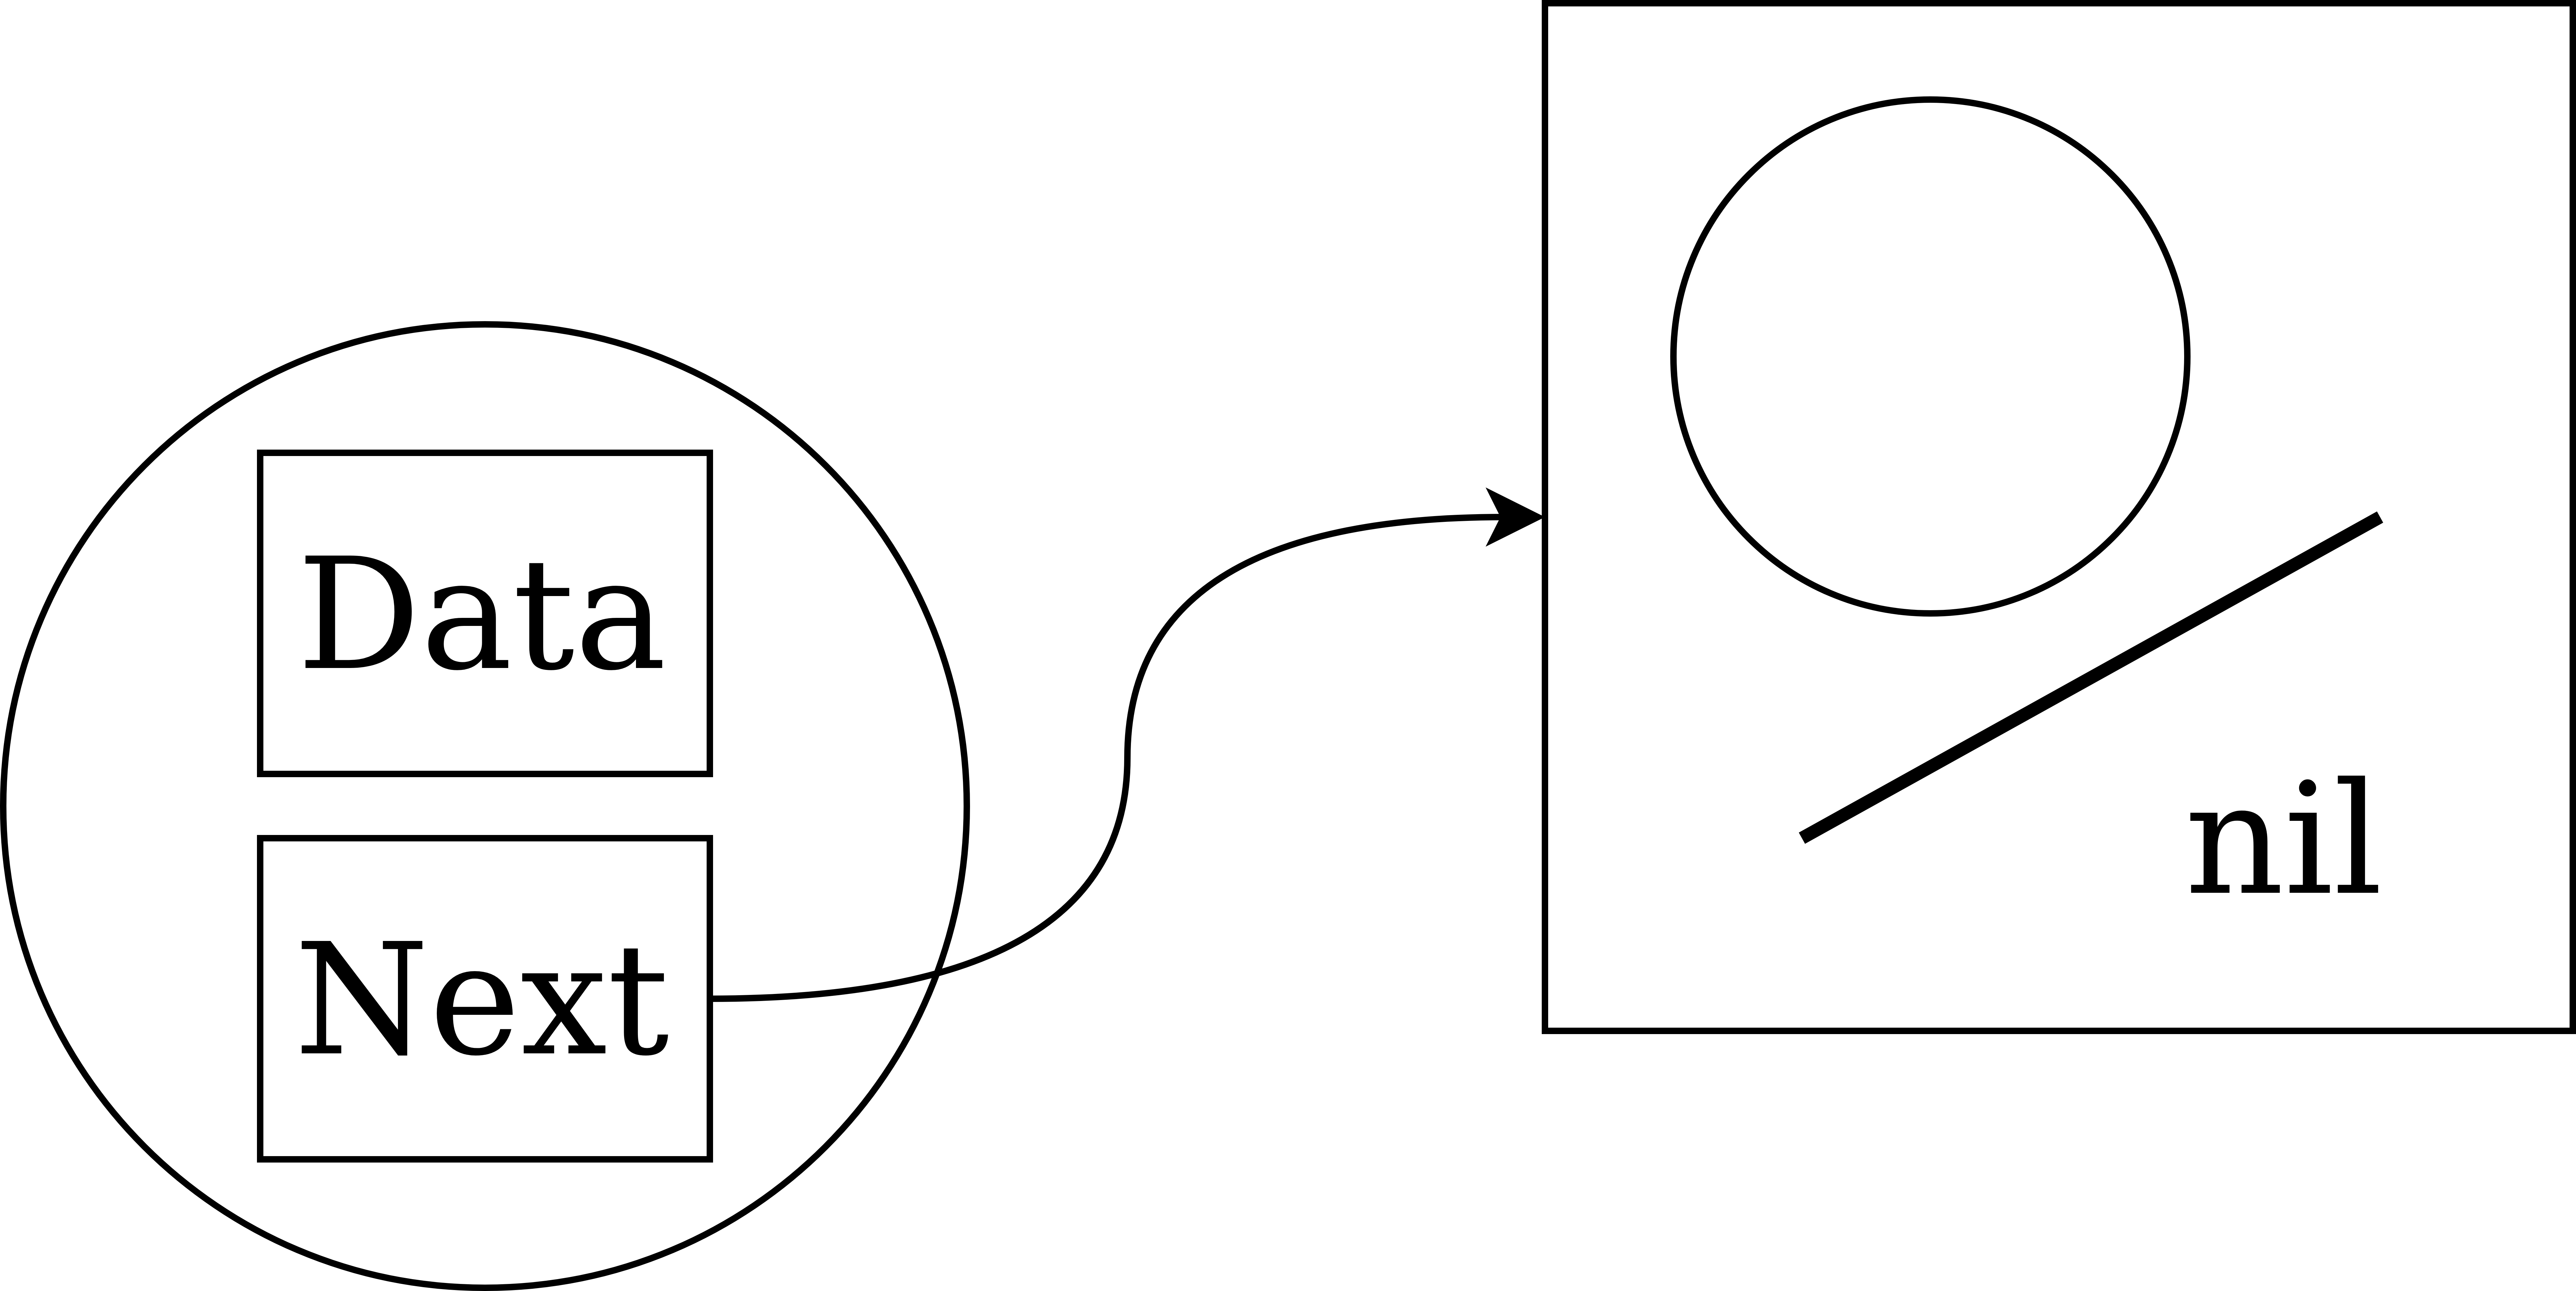
\includegraphics[width=0.5\linewidth]{pics/queue-node.png}
\end{figure}

\renewcommand{\lstlistingname}{Listing}
\begin{lstlisting}[caption={Queue node structure},label={queue-node-structure},escapeinside={(*}{*)}, captionpos=b]
type QueueNode = struct {
    Data: OperationDescriptor,
    Next: QueueNode*
}
\end{lstlisting}

For each queue we maintain two pointers: \texttt{Tail}, that points to the last node of the queue, and \texttt{Head}, that points to the node \emph{before} the first node of the queue (Fig.~\ref{queue-structure-pic}). Note that the node at \texttt{Head} pointer does not store any data, residing in the queue. This node is considered dummy and only the node at \texttt{Head.Next} pointer contains the first real descriptor in the queue.

\begin{figure}[H]
  \centering
  \caption{Queue structure}
  \label{queue-structure-pic}
  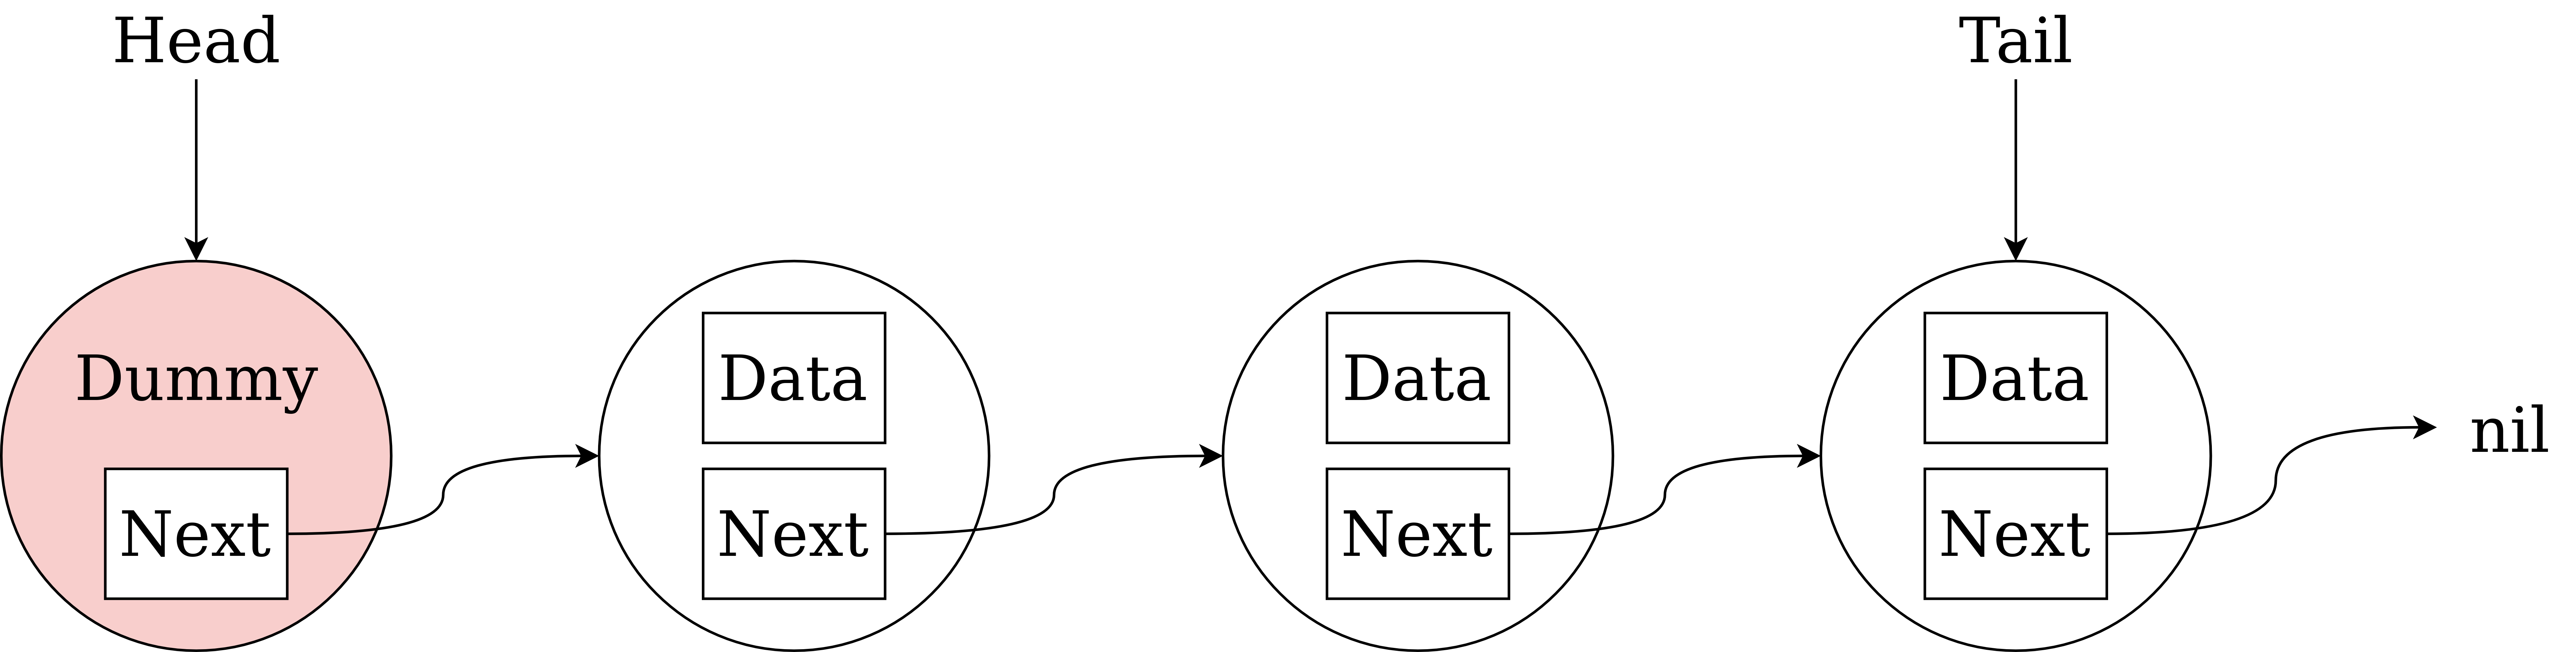
\includegraphics[width=\linewidth]{pics/queue-structure.png}
\end{figure}

An empty queue consists of a single dummy node, pointed at by both \texttt{Head} and \texttt{Tail} pointers (Fig.~\ref{empty-queue-structure-pic}).

\begin{figure}[H]
  \centering
  \caption{Empty queue structure}
  \label{empty-queue-structure-pic}
  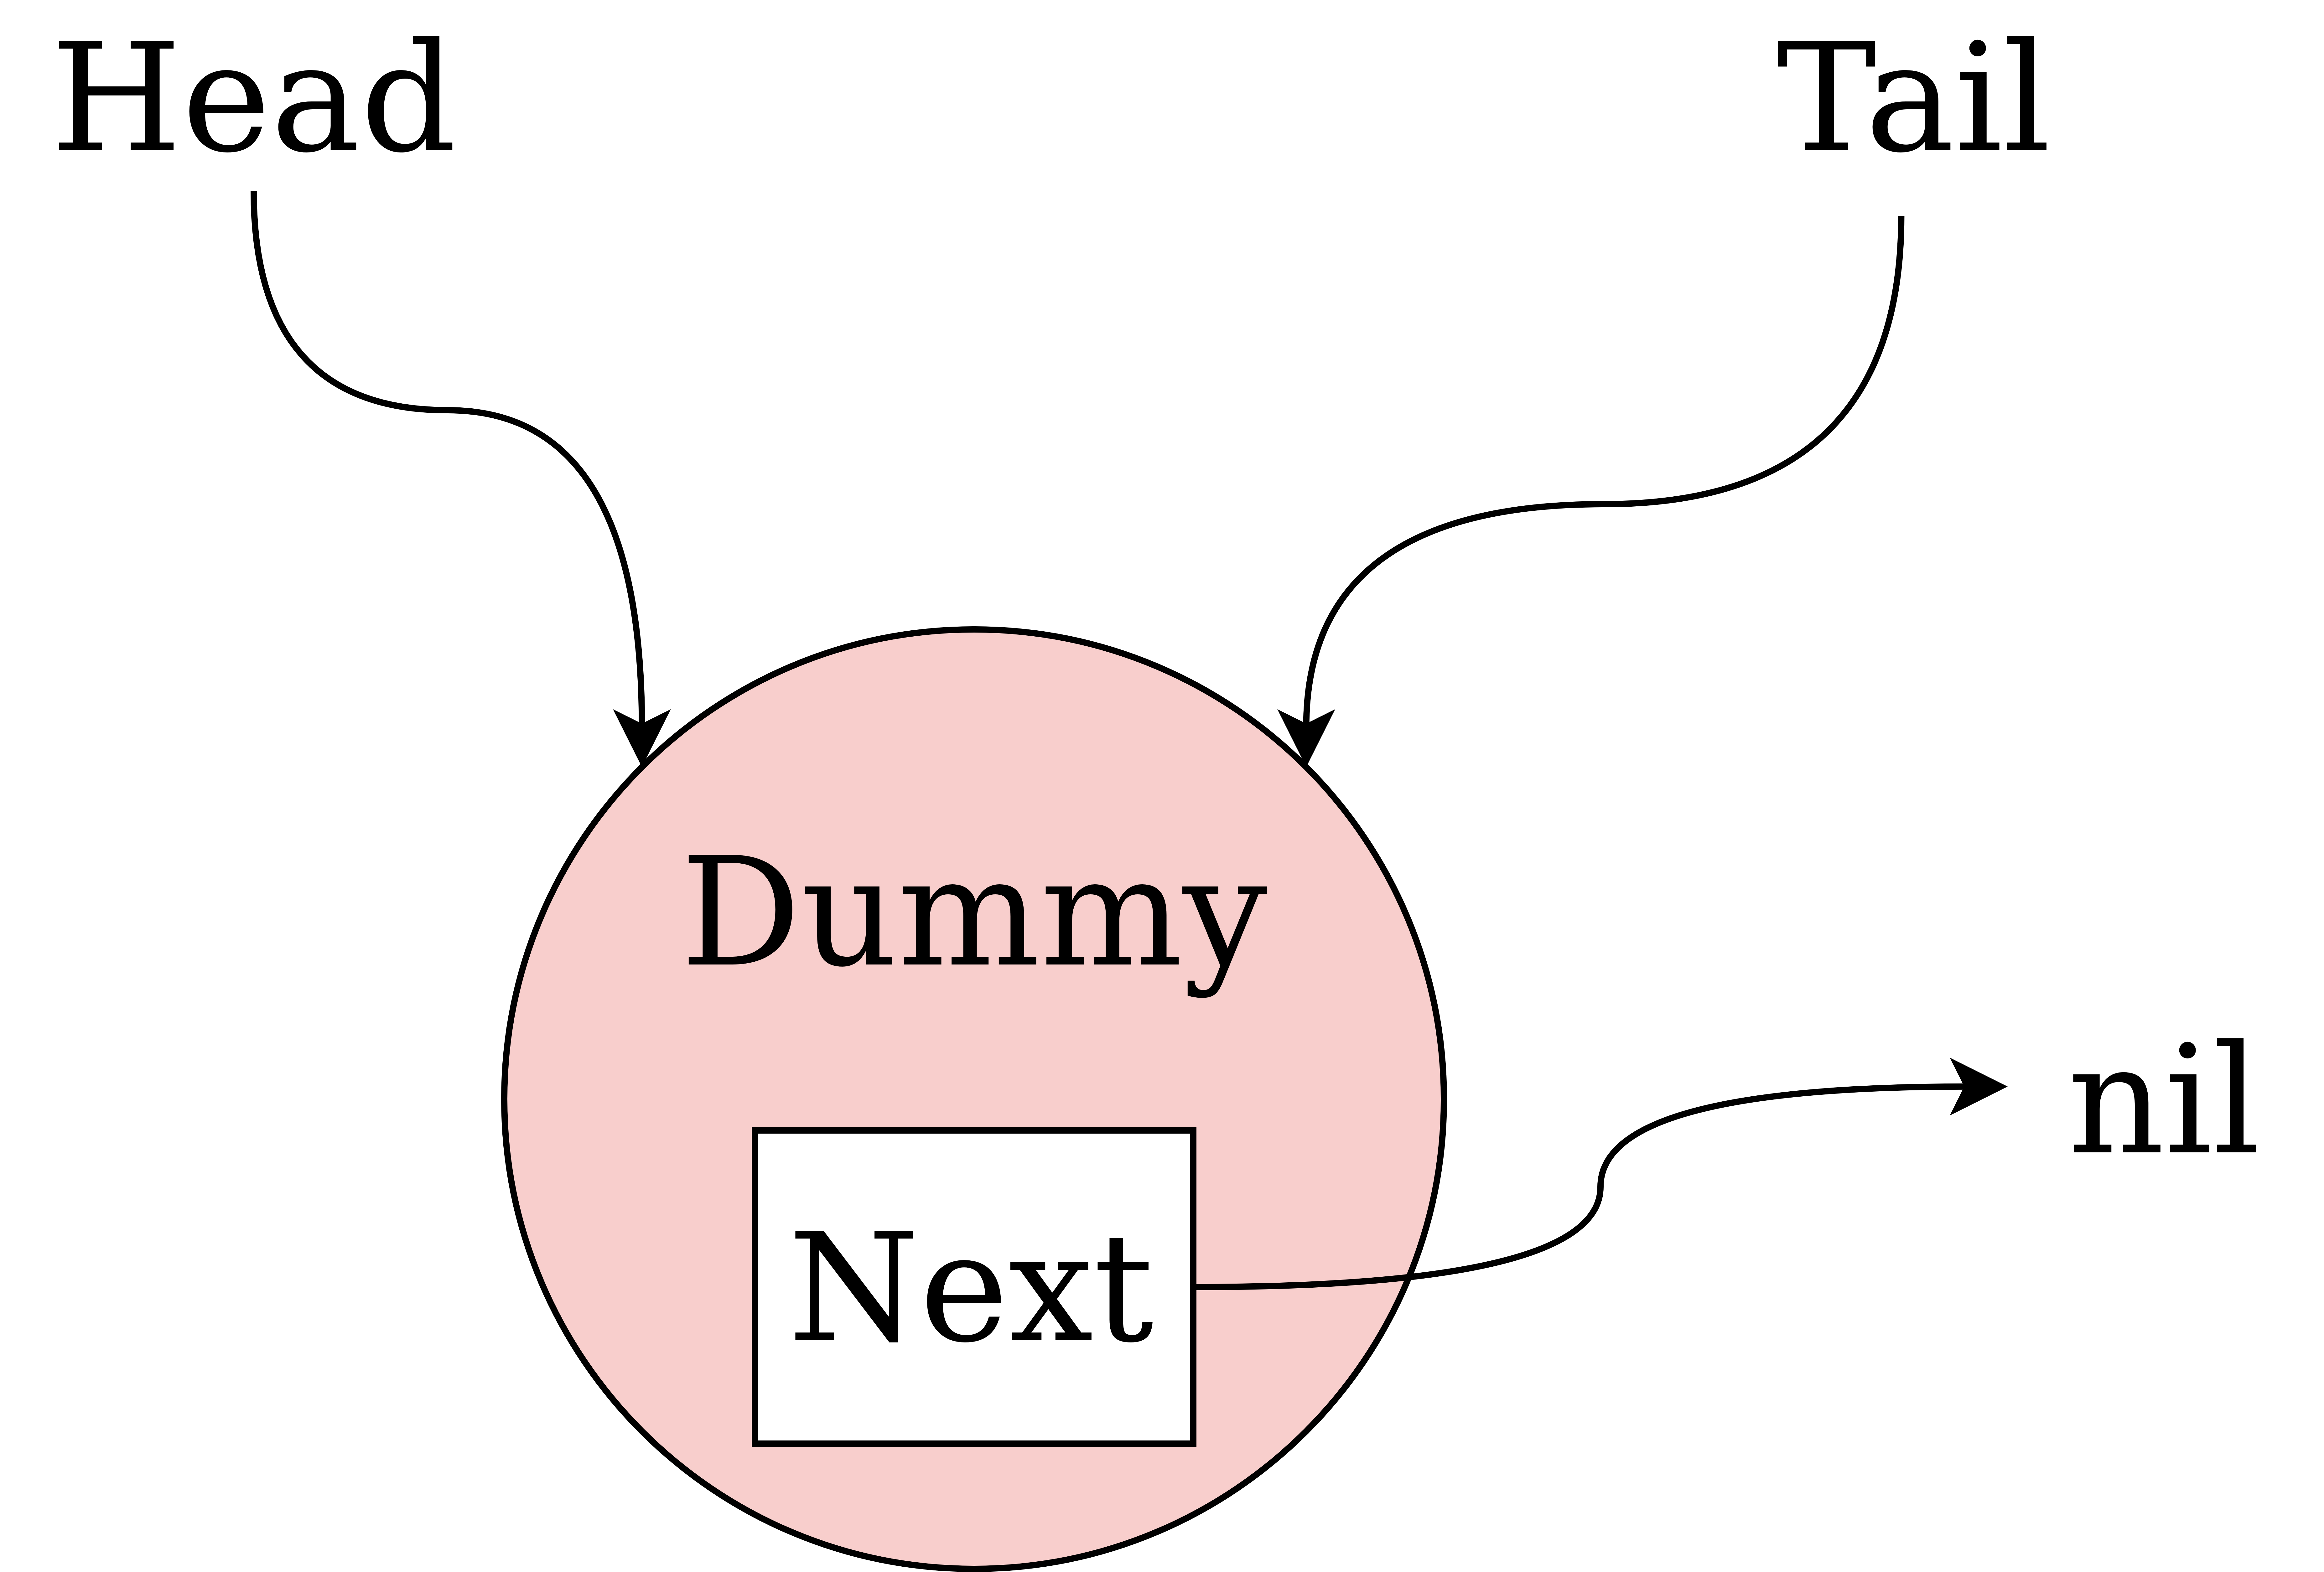
\includegraphics[width=0.5\linewidth]{pics/empty-queue-structure.png}
\end{figure}

\subsection{\texttt{push} with acquiring operation timestamp}
\label{push-acquire-timestamp-section}

As discussed in Section~\ref{main-invariant-chapter}, the operation queue in the root node should provide timestamp allocation mechanism, with the following guarantees: if the descriptor of operation \texttt{A} was added to the root queue before the descriptor of the operation \texttt{B}, then \texttt{timestamp(A) < timestamp(B)} should hold. 

Note, that the descriptor becomes visible to all the system processes at the moment it is added to the root queue, and, as described in Section~\ref{operation-execution-chapter}, the system processes examine timestamps of all descriptors in order to execute their operations. Thus, the timestamp should be written to the \texttt{descriptor.Timestamp} field before the descriptor is added to the root queue.

As was stated in Section~\ref{queue-structure-section}, we can use a slight modification of Michael-Scott queue~\cite{michael1996simple} to implement the timestanp alocation mechanism for the root queue.

The algorithm can be structured the following way:

\begin{nenum}
    \item Read \texttt{cur\_tail := Queue.Tail}~--- the current queue tail to learn the maximal allocated timestamp and start inserting the new descriptor to the tail of the queue. At this moment, multiple possible situations can happen:
    
    \begin{itemize}
        \item The queue is not empty and the tail points to the latest added descriptor (Fig.~\ref{root-queue-normal-pic}).
        
        \begin{figure}[H]
          \centering
          \caption{The queue is not empty and the tail points to the latest added descriptor}
          \label{root-queue-normal-pic}
          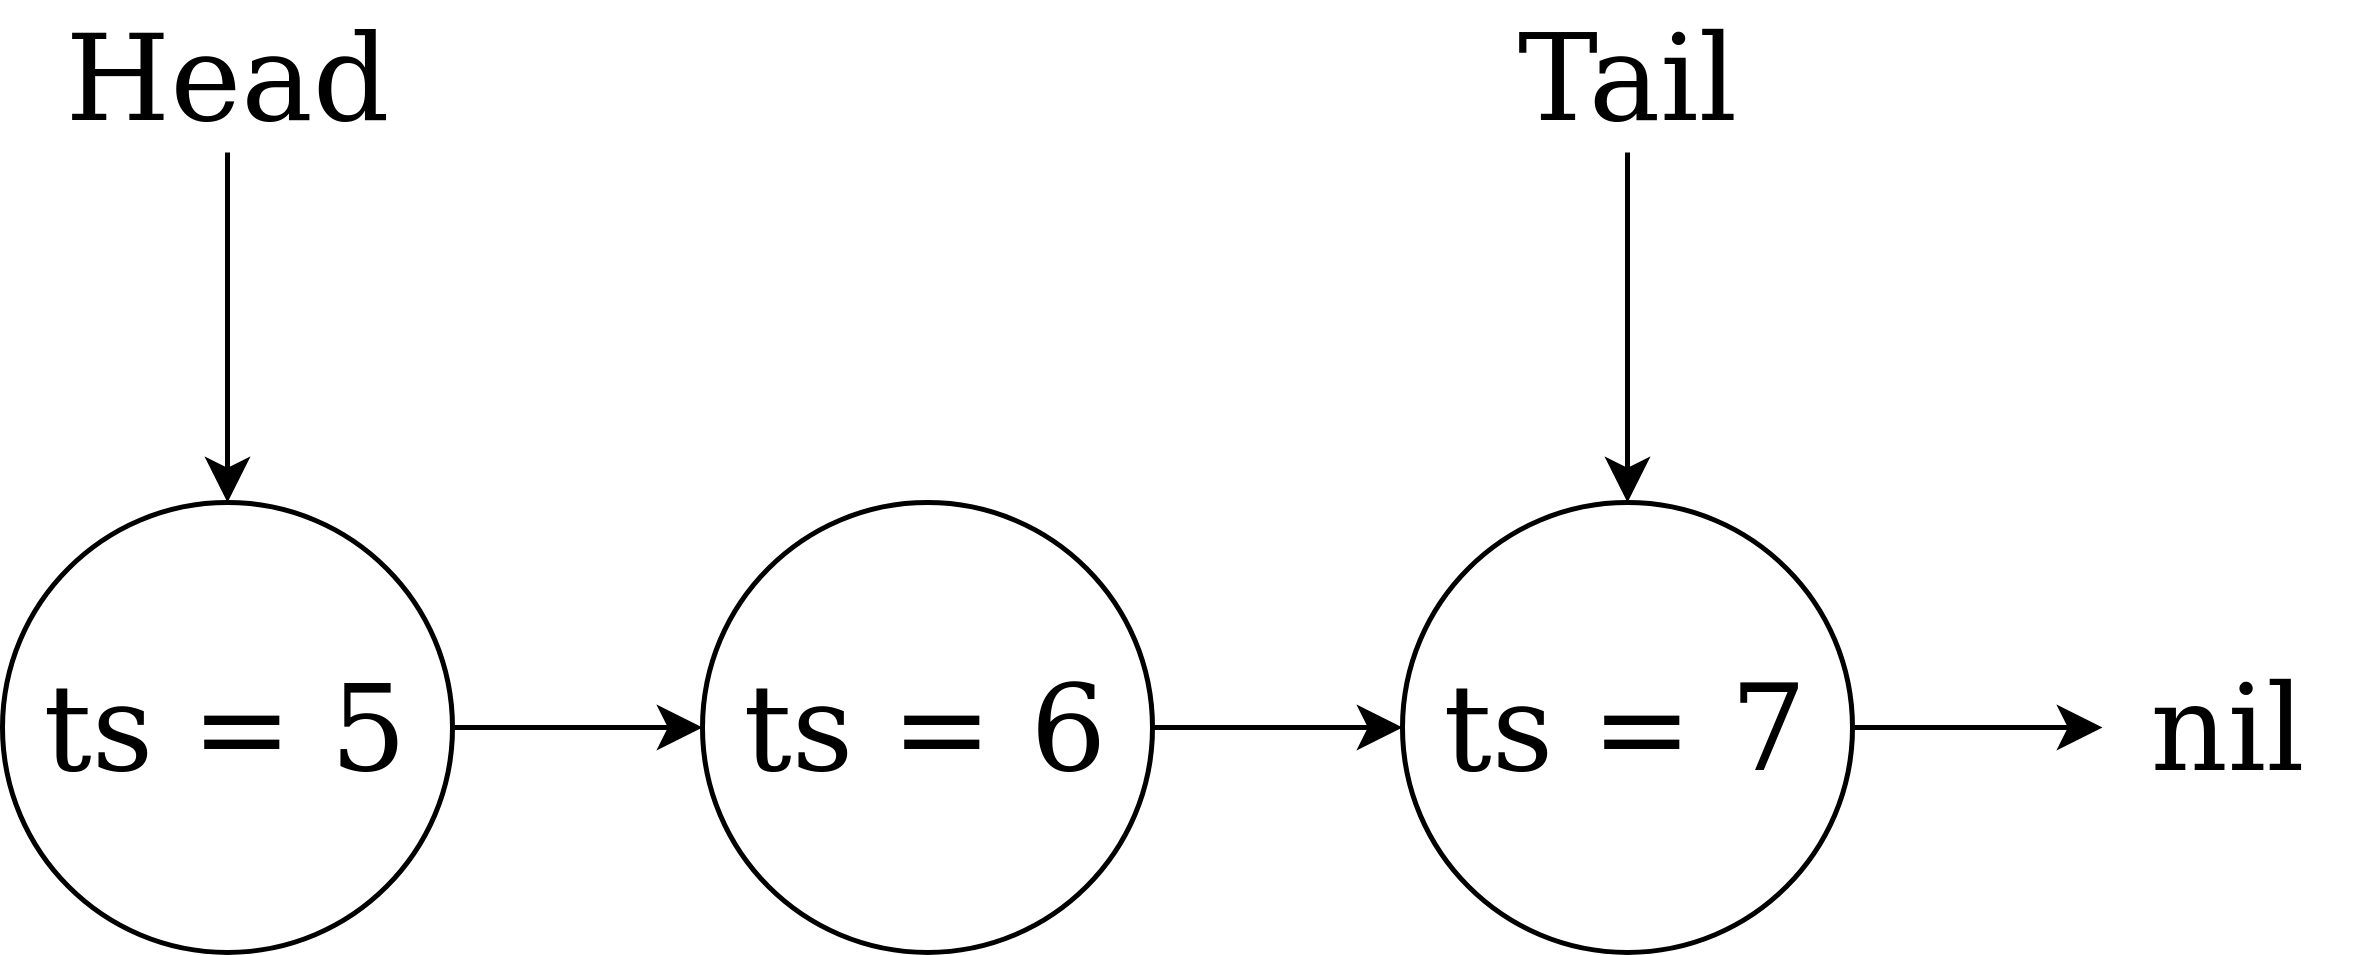
\includegraphics[width=0.7\linewidth]{pics/root-queue-normal.png}
        \end{figure}
        
        Thus, that descriptor contains the maximal timestamp, allocated by now and we can learn that timestamp by simply reading \texttt{cur\_tail.Data.Timestamp}
        
        \item The queue is empty, but at least one node has been added to it since the beginning of the execution (Fig.~\ref{root-queue-empty-non-dummy-pic}). In that case, \texttt{cur\_tail} points to the node that was the last removed from the queue, as guaranteed by the Michael-Scott queue structure~\cite{michael1996simple}. 
        
        \begin{figure}[H]
          \centering
          \caption{The queue is empty but it was non-empty at least once}
          \label{root-queue-empty-non-dummy-pic}
          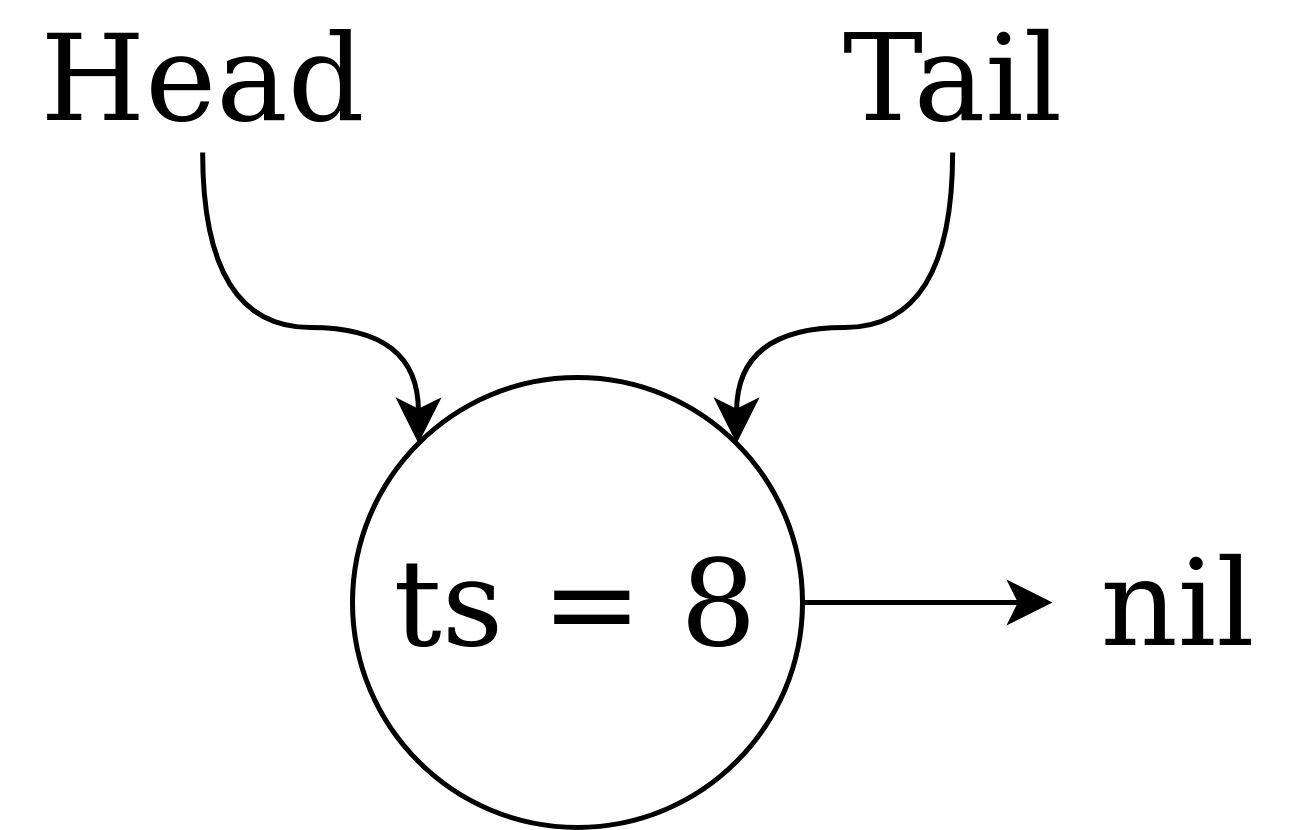
\includegraphics[width=0.7\linewidth]{pics/root-queue-empty-non-dummy.png}
        \end{figure}
        
        Therefore, the node, pointed at by \texttt{cur\_tail}, is the last node added to the queue, thus it contains the maximal allocated timestamp. Therefore, as in the previous case, we can learn the maximal allocated timestamp by reading \texttt{cur\_tail.Data.Timestamp}.
        
        \item The queue is empty and not a single node has been inserted to it since the beginning of the execution. In that case, the \texttt{cur\_tail} points at the dummy node, as guaranteed by the Michael-Scott queue structure~\cite{michael1996simple} and stated in Section~\ref{queue-structure-section} (Fig~\ref{root-queue-empty-dummy-pic}). 
        
        \begin{figure}[H]
          \centering
          \caption{The queue has always been empty}
          \label{root-queue-empty-dummy-pic}
          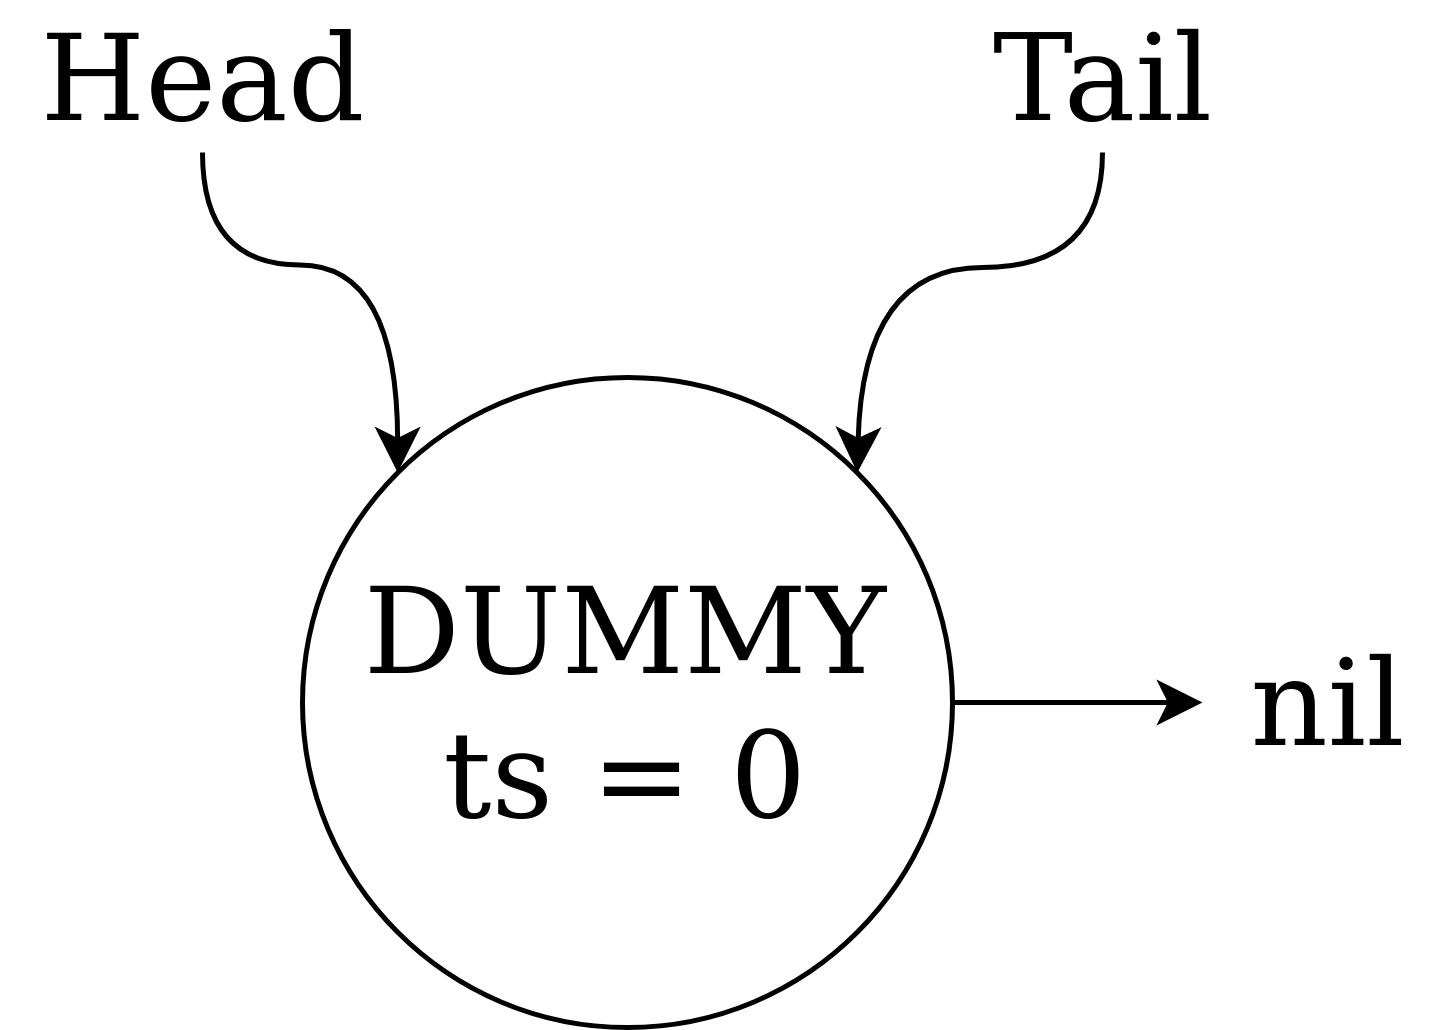
\includegraphics[width=0.5\linewidth]{pics/root-queue-empty-dummy.png}
        \end{figure}
        
        We may consider zero to be the maximal timestamp, allocated at the beginning of the execution. Thus, we construct a dummy node so that it contains zero as its timestamp (i.e. \texttt{Dummy\_Node.Data.Timestamp = 0}). Thus, yet again we we can learn the maximal allocated timestamp by reading \texttt{cur\_tail.Data.Timestamp}
        
        \item The queue is not empty and the tail does not point to the latest added descriptor (Fig.~\ref{root-queue-stale-tail-pic}). This can happen if another descriptor is being inserted to the queue concurrently.
        
        \begin{figure}[H]
          \centering
          \caption{The queue is not empty and the tail does not point to the latest added descriptor}
          \label{root-queue-stale-tail-pic}
          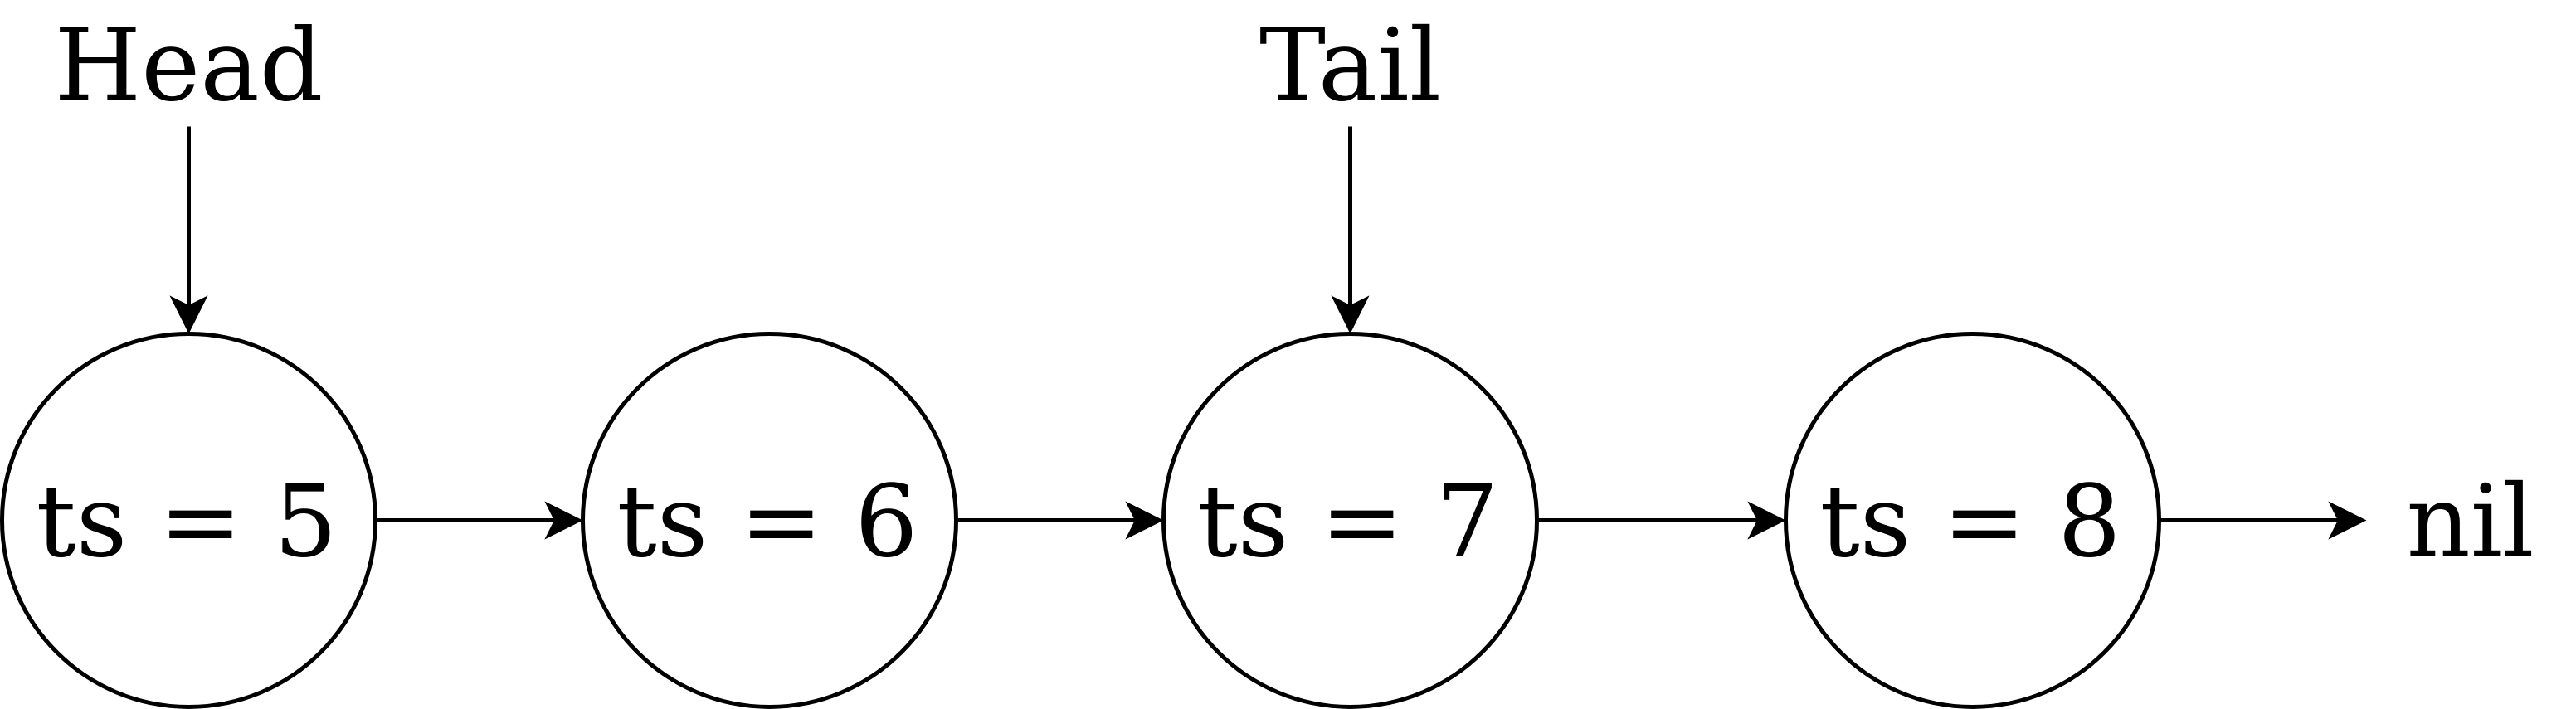
\includegraphics[width=0.7\linewidth]{pics/root-queue-stale-tail.png}
        \end{figure}
        
        In that case, as described later, we retry the whole procedure from the very beginning, i.e., from step (1). Thus, it does not matter, which timestamp we learn~--- for example, we may choose \texttt{cur\_tail.Data.Timestamp} to be the learned timestamp.
    \end{itemize}
    
    \bigbreak
    
    Therefore, in all possible cases we can learn the maximal allocated timestamp by reading \texttt{cur\_tail.Data.Timestamp}.
    
    \item After learning the maximal allocated timestamp, we set \texttt{new\_descriptor.Timestamp} equal to the the learned maximal timestamp incremented by one. Note, that this \texttt{write} operation is not concurrent with any \texttt{read} or \texttt{write} operation on \texttt{new\_descriptor}. Indeed, writing \texttt{new\_descriptor.Timestamp} is performed only by the initiator process on the \texttt{new\_descriptor} before it is inserted to the queue, and thus before the \texttt{new\_descriptor} becomes visible to other processes.
    
    \item We try to add the new descriptor to the tail of the queue the same way we insert elements to the Michael-Scott queue: we simply try to perform \texttt{CAS(\&cur\_tail.Next, nil, new\_node)}. We can have two possible outcomes of that \texttt{CAS}:
    
    \begin{itemize}
        \item If the \texttt{CAS} returns \texttt{false}, then some other process successfully inserted its descriptor to the tail of the queue thus modifying \texttt{cur\_tail.Next}. In that case, we help the successful process finish its insertion. We begin with reading \texttt{other\_process\_tail := cur\_tail.Next}, after that we try to move the queue tail forward by executing \texttt{CAS(\&Queue.Tail, cur\_tail, other\_process\_tail)} (Fig.~\ref{queue-move-tail-pic}). 
        
        \begin{figure}[H]
          \centering
          \caption{Moving the queue tail forward}
          \label{queue-move-tail-pic}
          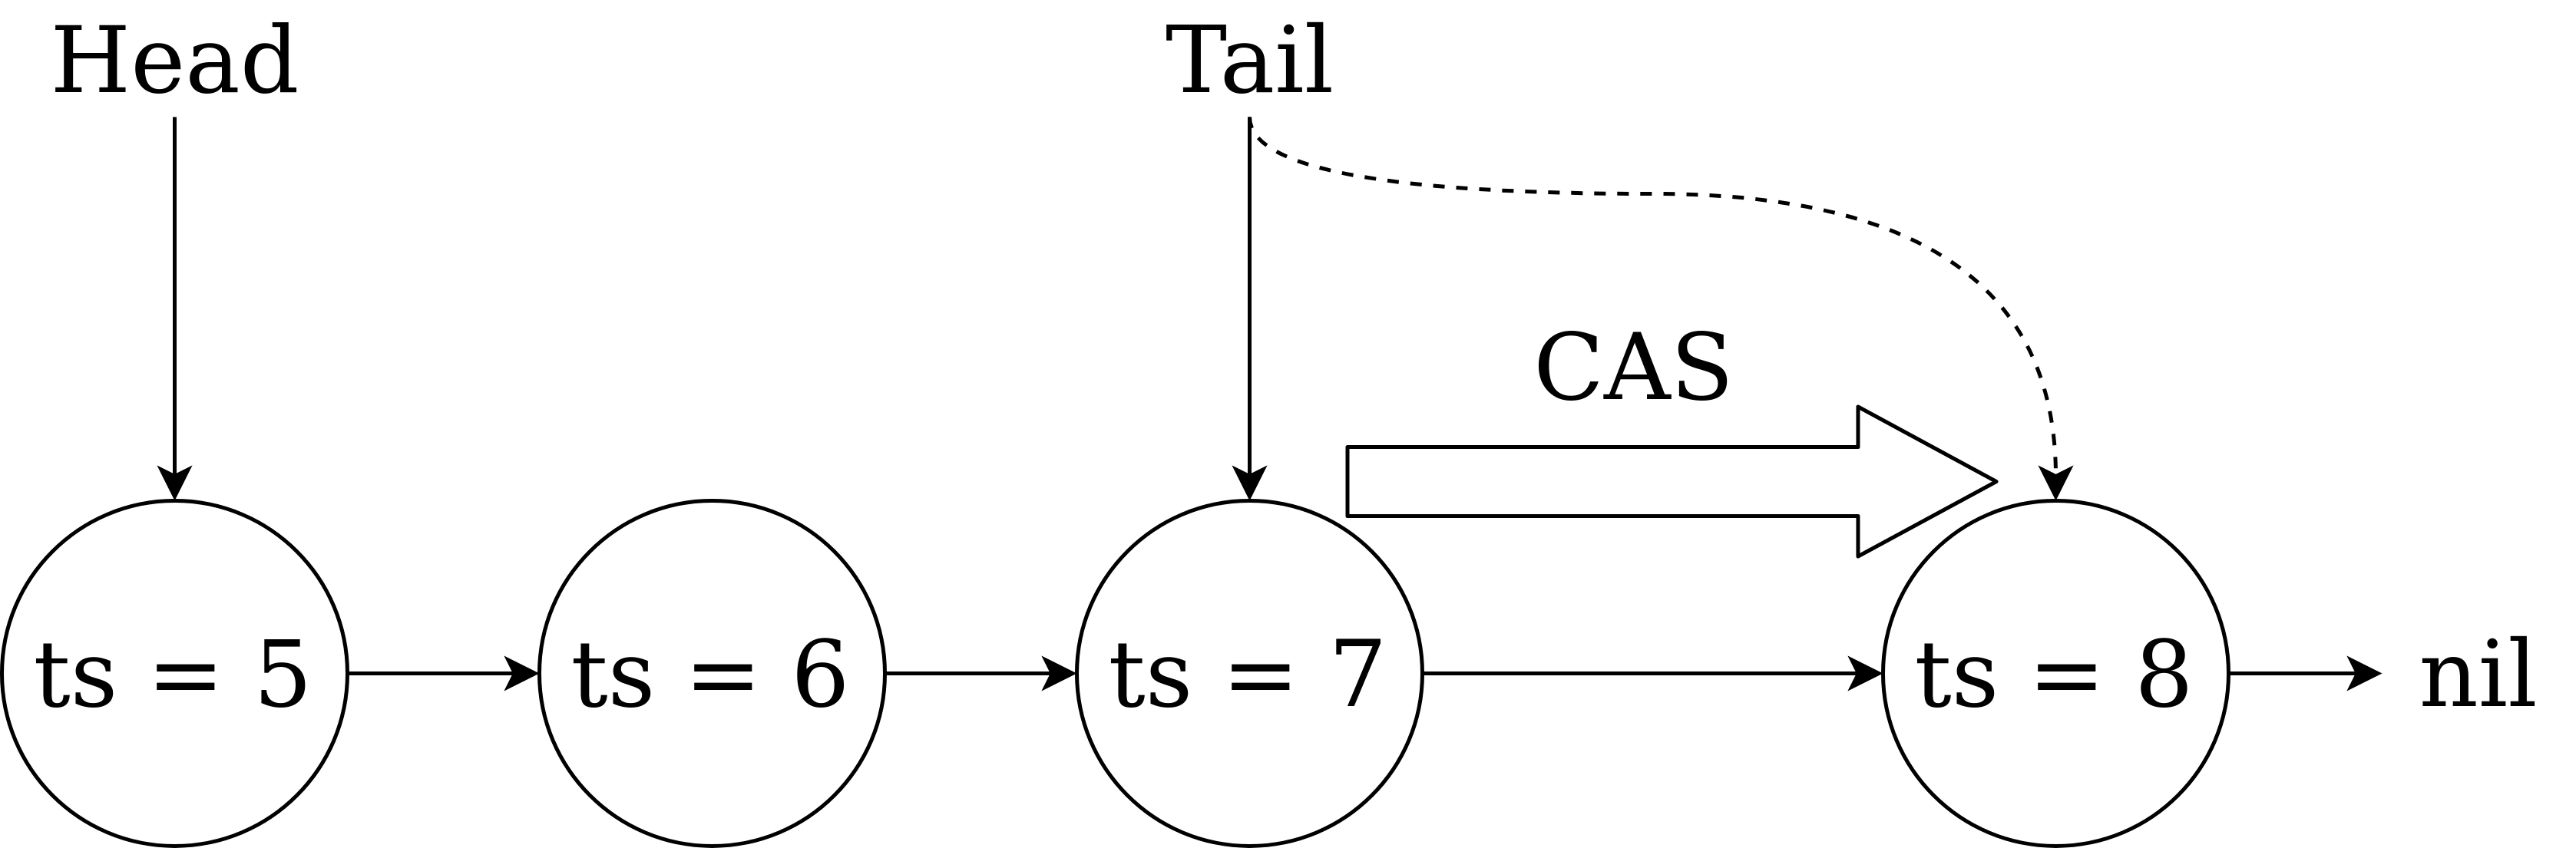
\includegraphics[width=\linewidth]{pics/queue-move-tail.png}
        \end{figure}
        
        As any \texttt{CAS}, that \texttt{CAS} can be either 1) successful~--- in that case we have helped the other process and moved the queue tail forward; 2) unsuccessful~--- in that case, some other process helped before us. In either case, we simply retry the whole procedure from the from step (1).
    
        \item If \texttt{CAS} returns \texttt{true}, we added the descriptor to the tail of the queue. In that case, as in the previous one, we should move the queue tail forward by \texttt{CAS(\&Queue.Tail, cur\_tail, new\_node)}. After that, we simply finish the insertion, no matter is the second \texttt{CAS} successful (if so, we moved \texttt{Queue.Tail} forward) or not (in that case, some other process moved it to help us, as described above).
    \end{itemize}
\end{nenum}

The algorithm can be implemented the following way (Listing~\ref{push-acquire-timestamp-listing}):

\renewcommand{\lstlistingname}{Listing}
\begin{lstlisting}[caption={Implementation of the \texttt{push} procedure with acquiring operation timestamp},label={push-acquire-timestamp-listing},escapeinside={(*}{*)}, captionpos=b]
/* 
Executed by the initiator process at the 
beginning of the operation execution 
*/
fun push_acquire_timestamp(Root_Queue, descriptor):
    new_node := new QueueNode(Data = descriptor, Next = nil)
    while true:
        cur_tail := Root_Queue.Tail
        max_timestamp := cur_tail.Data.Timestamp
        descriptor.Timestamp (*$\leftarrow$*) max_timestamp + 1
        if CAS(&cur_tail.Next, nil, new_node):
            CAS(&Root_Queue.Tail, cur_tail, new_node)
            return
        else:
            other_process_tail := cur_tail.Next
            CAS(&Root_Queue.Tail, cur_tail, other_process_tail)
            /* Retry the whole operation from the very beginning */
\end{lstlisting}

\subsection{\texttt{push\_if} implementation}
\label{push-if-section}

As discussed in Section~\ref{no-casn-chapter}, non-root queues should provide \texttt{push\_if} operation that inserts a descriptor into the queue if it was not inserted yet (otherwise, the queue should be left unmodified). Just like in the previous case, the procedure is based on the Michael-Scott queue insertion algorithm~\cite{michael1996simple} and can be implemented the following way:

\begin{nenum}
    \item We learn the current queue tail by reading \texttt{cur\_tail := Queue.Tail}; 
    
    \item We learn the maximal operation timestamp, that has ever been inserted to the queue. We do it the same way as in Section~\ref{push-acquire-timestamp-section}~--- by reading \texttt{cur\_queue.Data.Timestamp} value.
    
    \item If that timestamp is greater than or equal to \texttt{descriptor.Timestamp}, we can conclude that the descriptor was already inserted to the queue. Thus, we can simply finish the operation, leaving the queue unmodified. 
    
    As was stated in Section~\ref{push-acquire-timestamp-section}, we can learn the timestamp not from the last node, but from the penultimate node (Fig.~\ref{non-root-queue-stale-tail-pic}).
    
     \begin{figure}[H]
      \centering
      \caption{The queue tail does not point to the latest added descriptor}
      \label{non-root-queue-stale-tail-pic}
      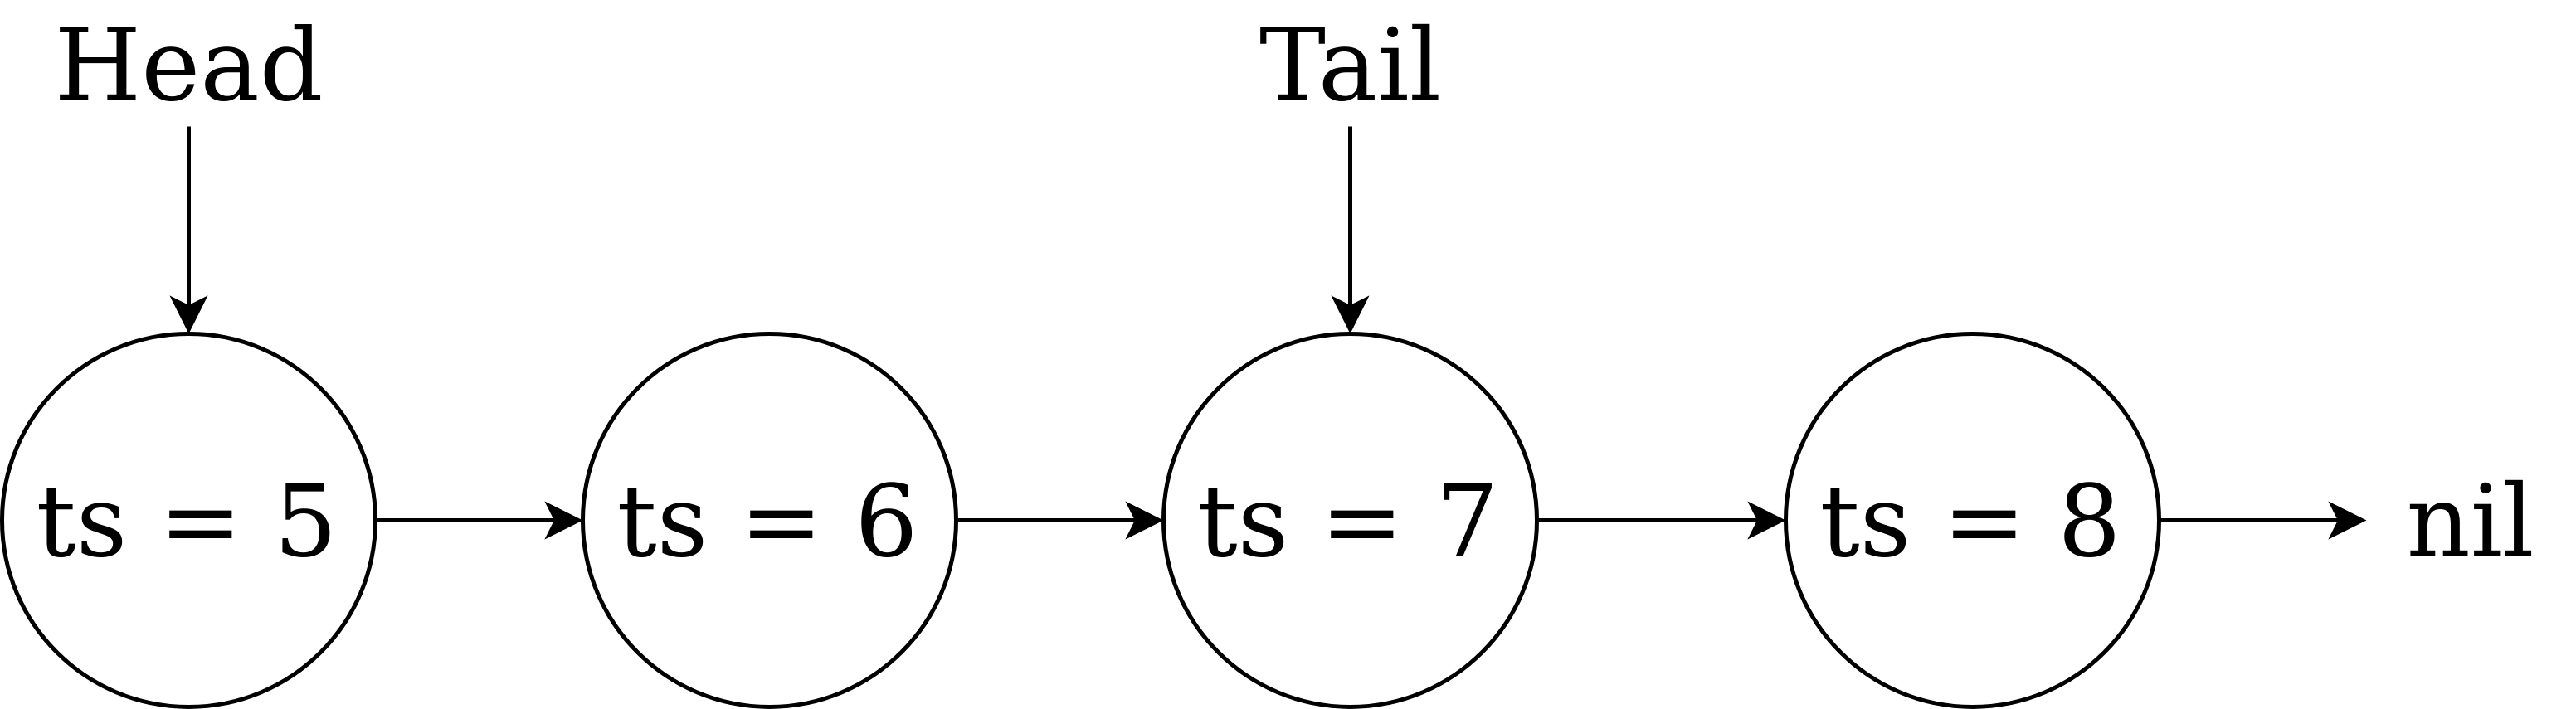
\includegraphics[width=0.7\linewidth]{pics/root-queue-stale-tail.png}
    \end{figure}
    
    Nevertheless, our conclusion remains the same: if at least one descriptor in the queue has \texttt{Timestamp $\geq$ descriptor.Timestamp} (even if the said descriptor is located in the penultimate queue node), it means that \texttt{descriptor} has already been inserted to the queue and we can simply finish the insertion.
    
    \item Otherwise, we try to insert the descriptor to the tail of the queue the same way, we did in Section~\ref{push-acquire-timestamp-section}. Note, that if the acquired \texttt{cur\_tail} pointer was pointing to the penultimate node, we shall simply retry the insertion from the very beginning.
\end{nenum}

\bigbreak

Therefore, the algorithm can be implemented the following way (Listing~\ref{push-if-listing}):

\renewcommand{\lstlistingname}{Listing}
\begin{lstlisting}[caption={Implementation of the \texttt{push\_if} procedure },label={push-if-listing},escapeinside={(*}{*)}, captionpos=b]
fun push_if(Non_Root_Queue, descriptor):
    new_node := new QueueNode(Data = descriptor, Next = nil)
    while true:
        cur_tail := Non_Root_Queue.Tail
        if cur_tail.Data.Timestamp (*$\geq$*) descriptor.Timestamp:
            return
        elif CAS(&cur_tail.Next, nil, new_node):
            CAS(&Non_Root_Queue.Tail, cur_tail, new_node)
            return
        else:
            other_process_tail := cur_tail.Next
            CAS(&Non_Root_Queue.Tail, cur_tail, other_process_tail)
            /* Retry the whole operation from the very beginning */
\end{lstlisting}

\subsection{\texttt{pop\_if} implementation}
\label{pop-if-section}

As discussed in Section~\ref{no-casn-chapter}, the operation queue in any node should provide \texttt{pop\_if} operation, that tries to remove descriptor with the specified timestamp \texttt{TS} from the head of the queue. If descriptor \texttt{D} with timestamp \texttt{TS} is still located at the head of the queue, it is removed (Fig.~\ref{pop-if-remove-pic}). Otherwise, the queue is left unmodified (Fig.~\ref{pop-if-not-remove-pic})~--- in this case, we assume that \texttt{D} was removed by some other process. We assume that at some moment \texttt{D} was located at the head of the queue (it may still be located at the head of the queue or it may be already removed), i.e., we never try to remove a descriptor from the middle of the queue (Fig.~\ref{pop-if-invalid-pic}).

\begin{figure}[H]
     \centering
     \begin{subfigure}[b]{0.45\linewidth}
          \centering
          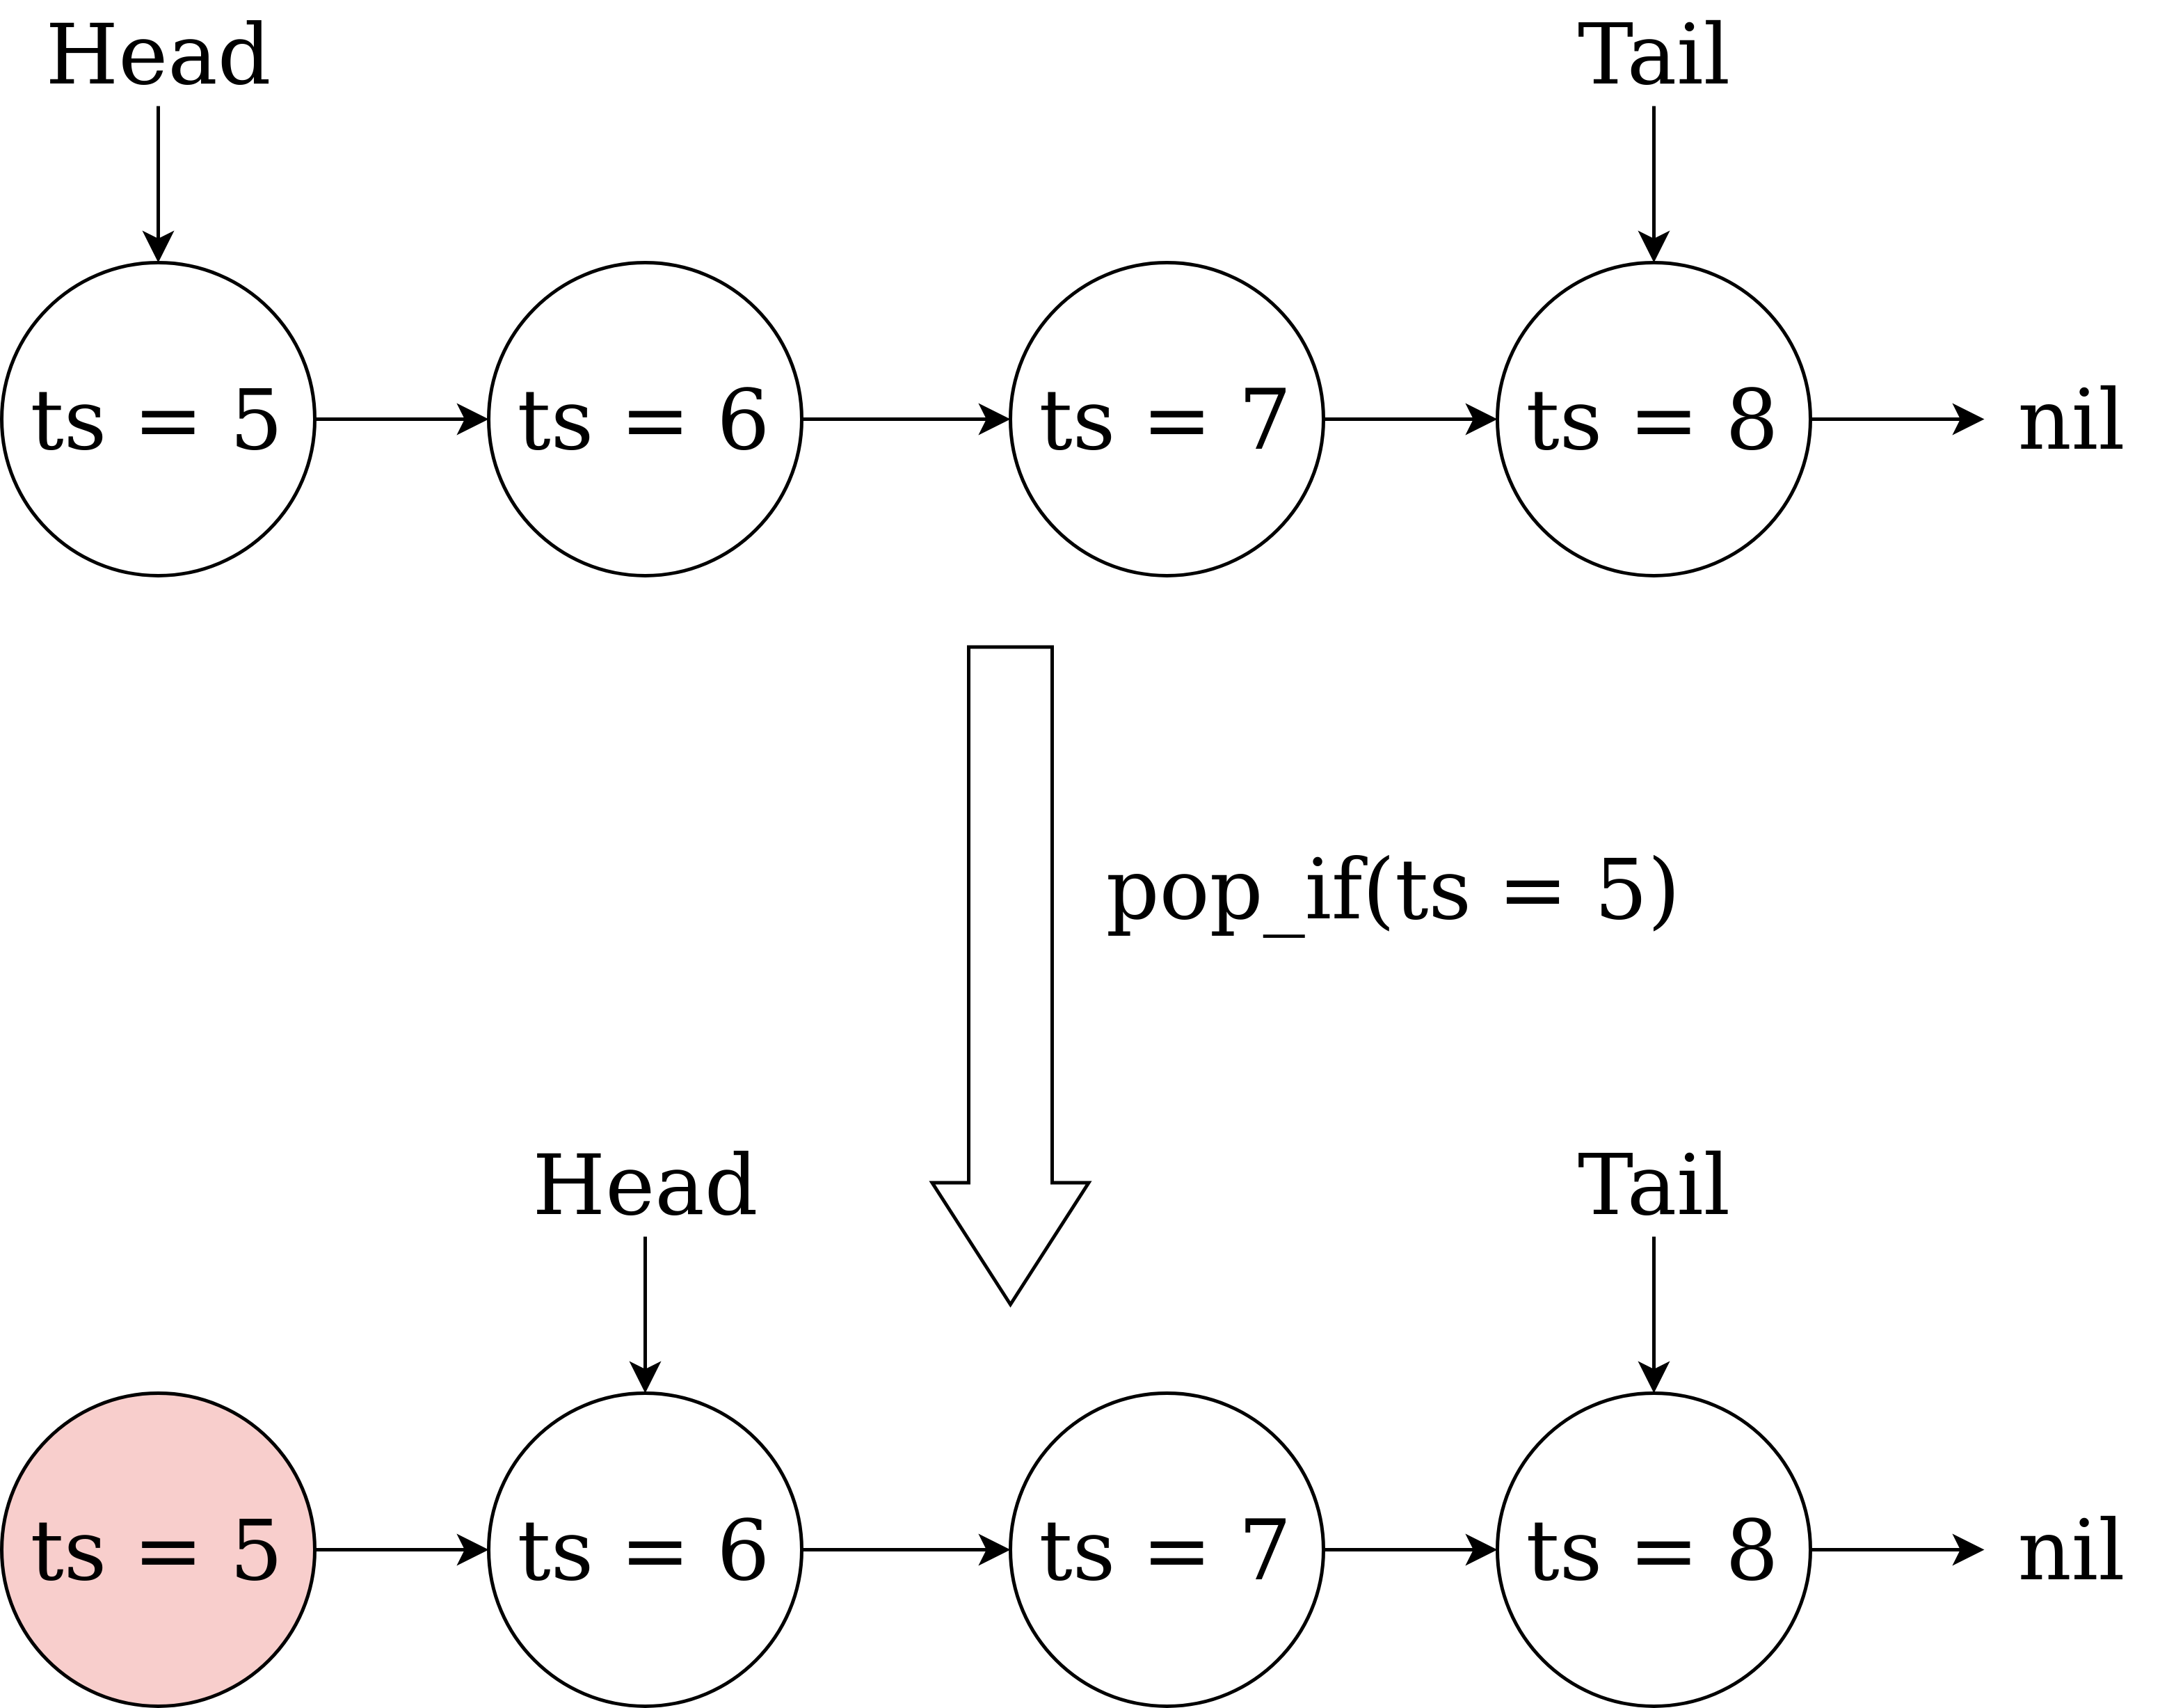
\includegraphics[width=\linewidth]{pics/pop-if-remove.png}
          \captionof{figure}{\texttt{pop\_if}: removing the descriptor from the head of the queue}
          \label{pop-if-remove-pic}
     \end{subfigure}
     \hfill
     \begin{subfigure}[b]{0.45\linewidth}
          \centering
          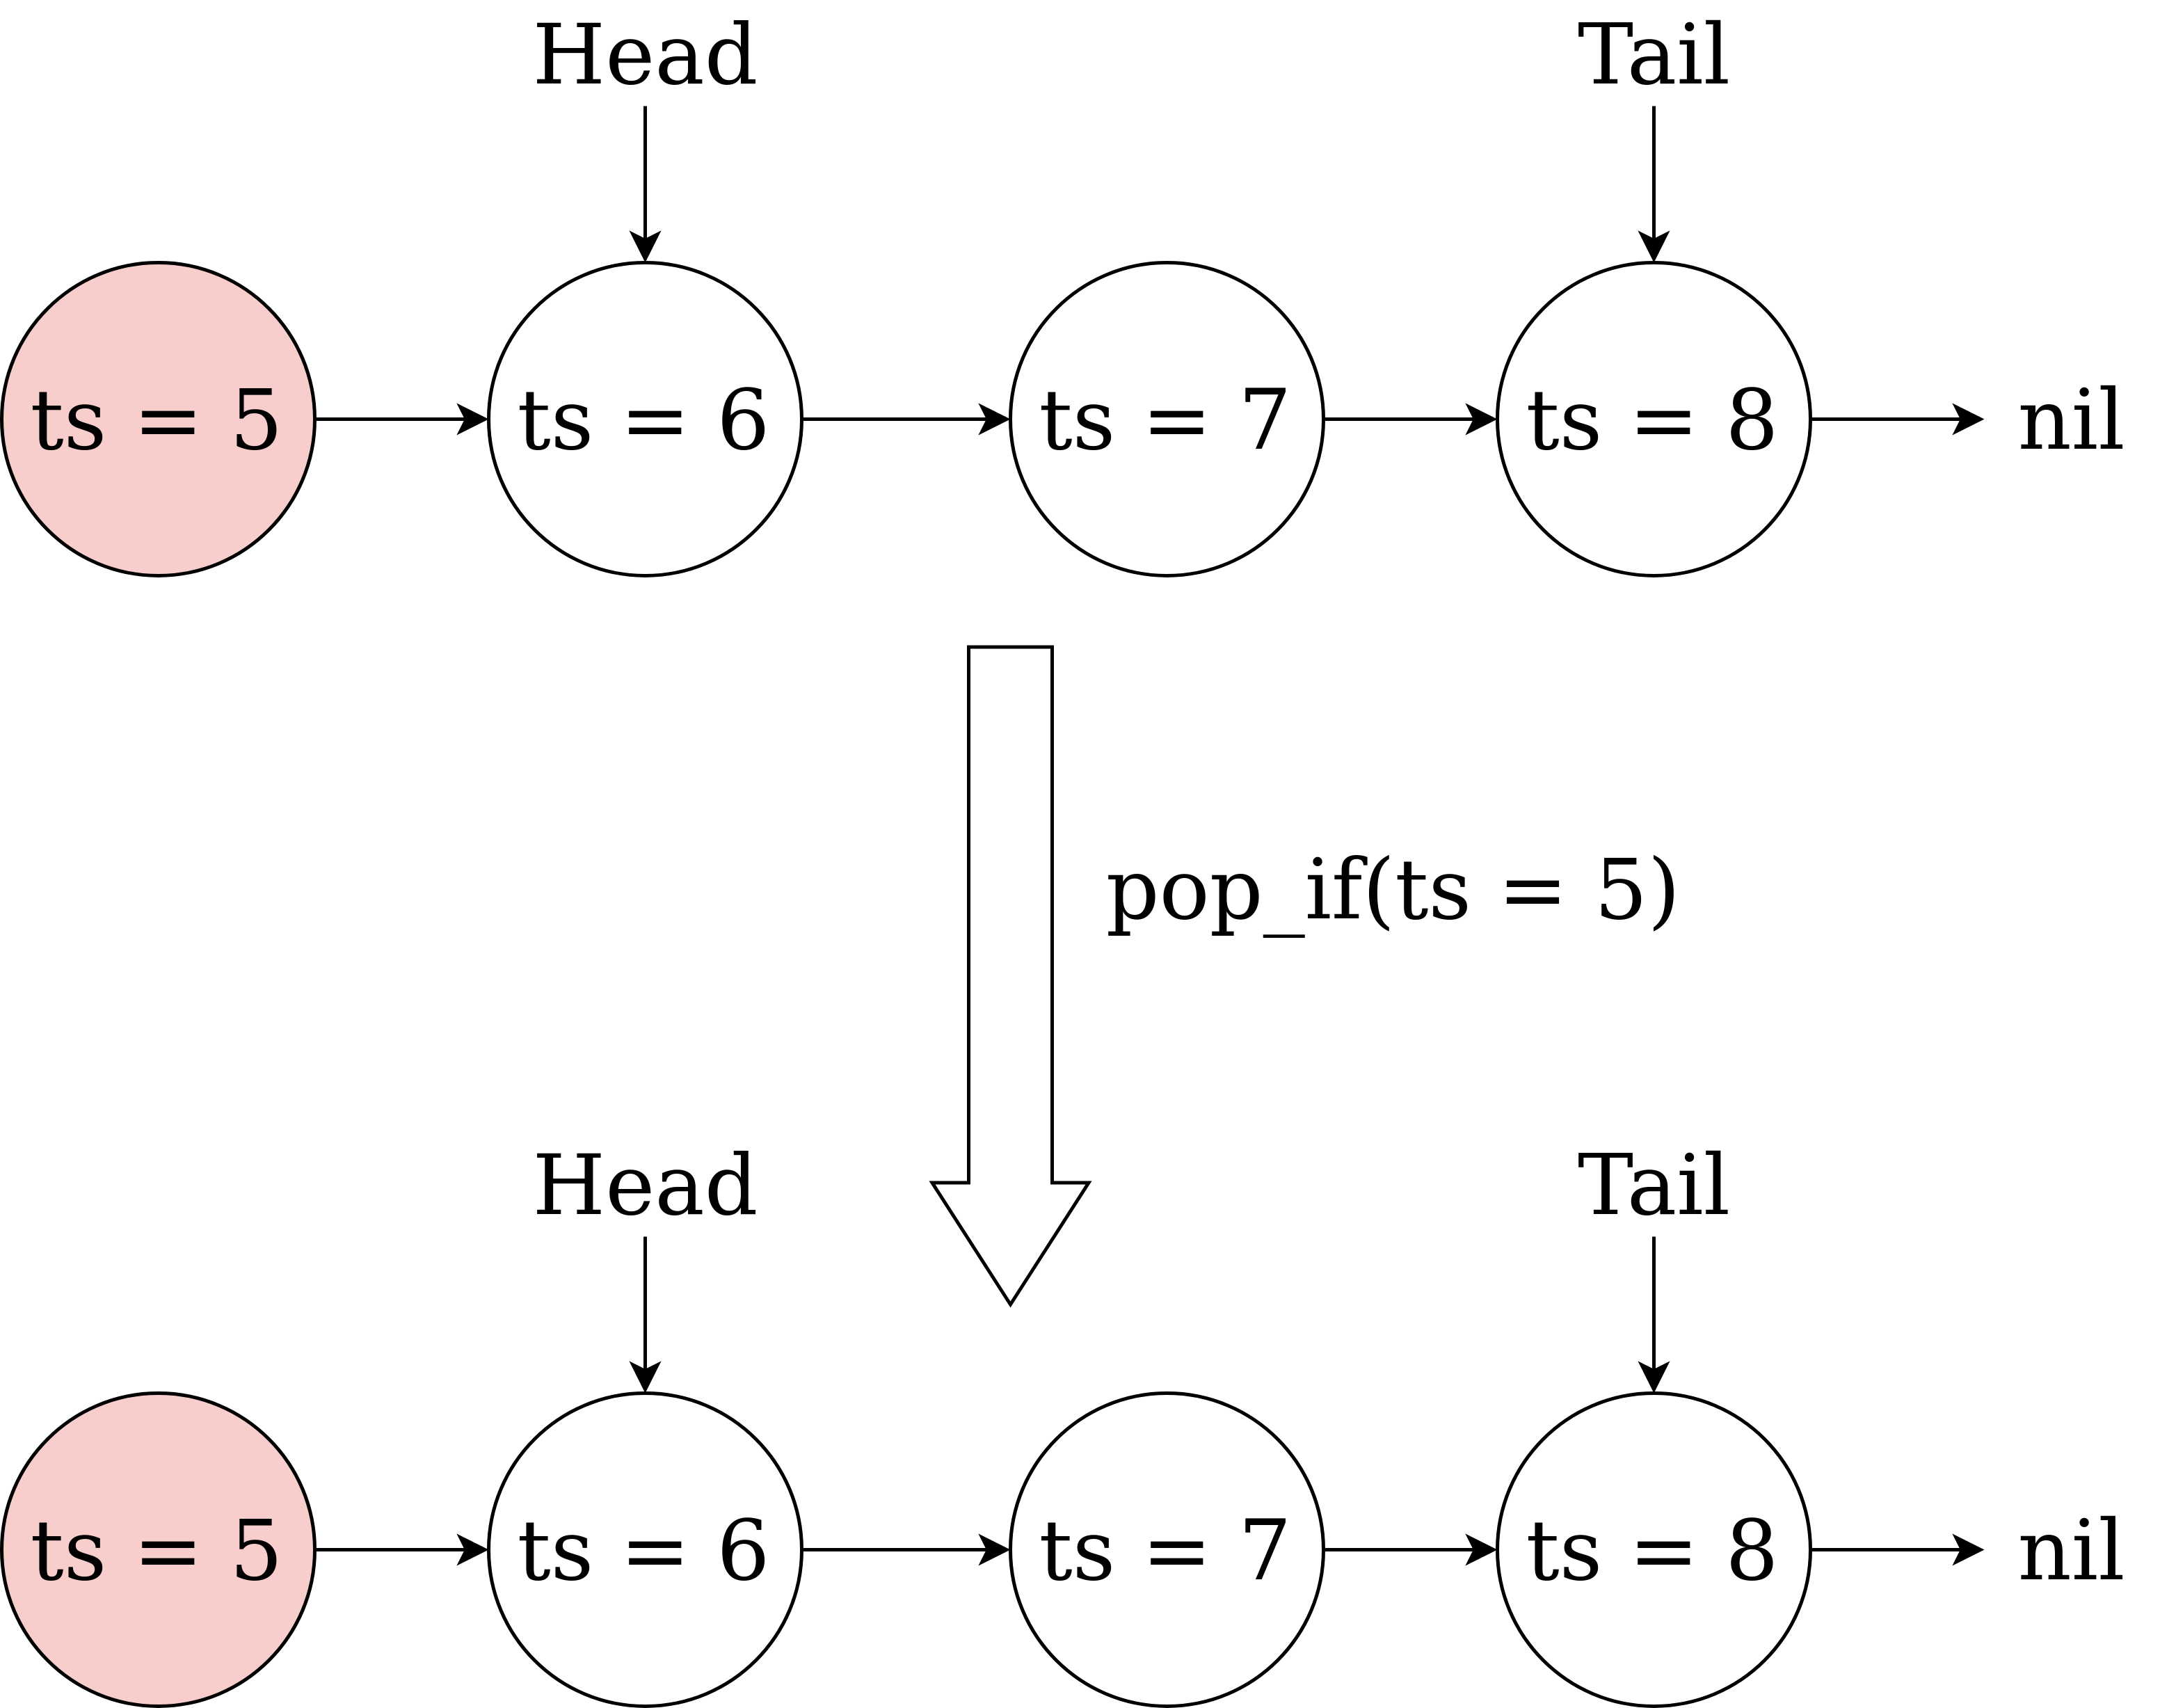
\includegraphics[width=\linewidth]{pics/pop-if-not-remove.png}
          \captionof{figure}{\texttt{pop\_if}: the descriptor has already been removed from the head of the queue, the queue is not modified}
          \label{pop-if-not-remove-pic}
     \end{subfigure}
     \hfill
     \begin{subfigure}[b]{0.45\linewidth}
          \centering
          \includegraphics[width=\linewidth]{pics/pop-if-invalid.png}
          \captionof{figure}{\texttt{pop\_if}: cannot try to remove a descriptor that was never located at the head of the queue}
          \label{pop-if-invalid-pic}
     \end{subfigure}
    \caption{Execution of \texttt{pop\_if} procedure for different queues}
    \label{pop-if-pics}
\end{figure}

Yet again, we can use slightly modified version of Michael-Scott queue~\cite{michael1996simple} to implement such a procedure in the following way:

\begin{nenum}
    \item Acquire head and tail nodes by reading \texttt{cur\_head := Queue.Head} and \texttt{cur\_tail := Queue.Tail}, respectively. According to the Michael-Scott queue structure~\cite{michael1996simple} the head node is a dummy node, that does not contain any data. Instead, the first descriptor is located at the node, pointed at by \texttt{cur\_head.Next} (Fig.~\ref{ms-queue-dummy-pic}). 
    
    \begin{figure}[H]
      \centering
      \caption{The head node is a dummy node that does not store any data}
      \label{ms-queue-dummy-pic}
      \includegraphics[width=\linewidth]{pics/ms-queue-dummy.png}
    \end{figure}
    
    \item If \texttt{cur\_head} and \texttt{cur\_tail} point to a single node, queue may be empty. In that case, to distinguish empty queue from non-empty, we read \texttt{cur\_tail.Next}. Two possible situations can happen:
    
    \begin{itemize}
        \item \texttt{cur\_tail.Next = nil} (Fig.~\ref{queue-pop-empty-pic}). In that case, the queue is empty and we finish the procedure, leaving the queue unmodified~--- we cannot remove the node from an empty queue. We can conclude that the descriptor was already removed by another process. 
        
        \begin{figure}[H]
          \centering
          \caption{The queue is empty}
          \label{queue-pop-empty-pic}
          \includegraphics[width=0.5\linewidth]{pics/queue-pop-empty.png}
        \end{figure}
        
        \item \texttt{cur\_tail.Next $\neq$ nil} (Fig.~\ref{queue-pop-restart-pic}). In that case,the  queue is not empty since new descriptor is being concurrently inserted to the queue. We should help finish the insertion by trying to move \texttt{Queue.Tail} forward the same way that was described in Section~\ref{push-acquire-timestamp-section}. 
        
        \begin{figure}[H]
          \centering
          \caption{The queue is not empty, we move the queue tail forward}
          \label{queue-pop-restart-pic}
          \includegraphics[width=0.7\linewidth]{pics/queue-pop-restart.png}
        \end{figure}
        
        After that, we simply retry the the \texttt{pop\_if} procedure from the very beginning, i.e., from step (1).
    \end{itemize}
    
    \item If \texttt{cur\_head} and \texttt{cur\_tail} point to different nodes, we continue executing the operation. We begin with reading \texttt{first\_timestamp}~--- timestamp of the first descriptor of the queue. The said timestamp can be acquired in \texttt{next\_head := cur\_head.Next} node (Fig.~\ref{pop-structure-pic}).
    
     \begin{figure}[H]
      \centering
      \caption{Acquiring \texttt{first\_timestamp}}
      \label{pop-structure-pic}
      \includegraphics[width=\linewidth]{pics/pop-structure.png}
    \end{figure}
    
    \begin{itemize}
        \item If \texttt{first\_timestamp $>$ TS} (e.g., is \texttt{TS = 4}), we can conclude that the descriptor with timestamp \texttt{TS} has already been removed by another process. Thus, we simply finish the \texttt{pop\_if} procedure leaving the queue unmodified.
    
        \item Otherwise, \texttt{first\_timestamp $=$ TS}. Note that \texttt{first\_timestamp} cannot be less than \texttt{TS} since, as was stated above, we never try to remove a node, that has never been located at the head of the queue. 
        
        In that case, we try to move the queue head forward by executing \texttt{CAS(\&Queue.Head, cur\_head, next\_head)}. If the \texttt{CAS} succeeds, we conclude that we have removed the requested descriptor from the queue and finish the operation. Otherwise, we conclude that some other process removed the requested descriptor and modified \texttt{Queue.Head}. In that case, we yet again simply finish the execution of the procedure.
    \end{itemize}
\end{nenum}

Therefore, \texttt{pop\_if} can be implemented in the following way (Listing~\ref{pop-if-listing}):

\renewcommand{\lstlistingname}{Listing}
\begin{lstlisting}[caption={Implementation of the \texttt{pop\_if} procedure },label={pop-if-listing},escapeinside={(*}{*)}, captionpos=b]
fun pop_if(Queue, timestamp):
    while true:
        cur_head := Queue.Head
        cur_tail := Queue.Tail
        if cur_head = cur_tail:
            next_tail := cur_tail.Next
            if next_tail = nil:
                return
            else:
                CAS(&Queue.Tail, cur_tail, next_tail)
                /* Retry the operation from the very beginning */
        else:
            next_head := cur_head.Next
            first_timestamp := next_head.Data.Timestamp
            if first_timestamp = timestamp:
                CAS(&Queue.Head, cur_head, next_head)
            return
\end{lstlisting}

\subsection{Queues progress guarantees and implementation details}

Note that all the queue operations described above are lock-free, just like in the original queue by Michael and Scott~\cite{michael1996simple}. Indeed, the repetition of each procedure from the very beginning indicates that other process successfully executed its procedure, thus modifying the queue.

Of course, we can take other queue algorithms as a basis for our solution, not only the one proposed by Michael and Scott. For example, we can use \texttt{fetch-and-add} queue, proposed by Yang et al.~\cite{yang2016wait} or practical wait-free queue, proposed by Kogan and Petrank~\cite{kogan2011wait}: \texttt{pop\_if}, \texttt{push\_if}, and \texttt{push\_acquire\_timestamp} implementation principles remain the same. We use Michael-Scott queue only due to the simplicity of its implementation. 

\section{One possible tree balancing strategy}
\label{balancing-section}

Until now, we considered only unbalanced trees. However, using unbalanced trees may result in $height \in \omega(\log N)$. Since most of the queries (e.g., \texttt{insert}, \texttt{remove} or \texttt{contains}) are executed on a tree in $\Theta(height)$ time, using unbalanced trees may result in these queries being executed in non-optimal $\omega(\log N)$ time. Therefore, we must design an algorithm to keep the tree balanced. One possible balancing strategy is based on subtree rebuilding and is similar to the balancing strategy proposed in \cite{brown2020non}. The idea of this approach can be formulated the following way: when the number of modifications, applied to a particular subtree, exceeds a threshold, we completely rebuild that subtree, making it perfectly balanced (Fig~\ref{rebuild-idea-pic}).

\begin{figure}[H]
  \centering
  \caption{Tree balancing via subtree rebuilding: when the number of modifications, applied to a subtree, exceeds a threshold, we rebuild the whole subtree}
  \label{rebuild-idea-pic}
  \includegraphics[width=\linewidth]{pics/rebuild-idea.png}
\end{figure}

For each tree node we maintain \texttt{Mod\_Cnt}~--- the number of modifications, applied to the subtree of this node. We store \texttt{Mod\_Cnt} in the node state. Moreover, for each node we store an immutable number \texttt{Init\_Sz}~--- initial size of its subtree, i.e., the number of data items in that node subtree at the moment of node creation (node can be created when a new data item is inserted to the tree or when the subtree, where the node is located, is rebuilt). We rebuild the node subtree when \texttt{Mod\_Cnt > K $\cdot$ Init\_Sz}, where \texttt{K} is a predefined constant.

We check whether the subtree of node \texttt{v} needs rebuilding (and perform the rebuilding itself) only before inserting an operation descriptor to \texttt{v} queue and changing \texttt{v} state. Therefore, we can perform \texttt{v} subtree rebuilding only during execution of some operation in \texttt{v} parent. 

Consider node \texttt{v}, its parent \texttt{pv} and operation \texttt{Op}, that is being executed in \texttt{pv} and that should continue its execution in \texttt{v} subtree (and, therefore, its descriptor should be inserted to \texttt{v} queue). Before inserting \texttt{Op} to \texttt{v} queue and changing \texttt{v} state, we check whether \texttt{Mod\_Cnt} in \texttt{v} will exceed the threshold after applying \texttt{Op} to \texttt{v} subtree (Fig.~\ref{rebuild-when-pic}). 

\begin{figure}[H]
  \centering
  \caption{We check whether the subtree of \texttt{v} should be rebuilt or not}
  \label{rebuild-when-pic}
  \includegraphics[width=\linewidth]{pics/rebuild-when.png}
\end{figure}

The algorithm for the check whether the subtree of \texttt{v} should be rebuilt or not, is the following:

\begin{nenum}
    \item If \texttt{Op} is not a modifying operation (i.e. \texttt{Op} is a read-only operation), e.g., \texttt{contains} or \texttt{count}, we should not rebuild \texttt{v} subtree, since \texttt{Op} does not increase the number of modifications after being applied to \texttt{v} subtree.
    
    \item Otherwise, atomically read \texttt{v} state.
    
    \item If \texttt{Ts\_Mod $\geq$ Op.Timestamp}, then \texttt{v} state has already been modified by \texttt{Op}. Thus, \texttt{Op} has already been counted in the number of modifications, applied to \texttt{v} subtree and we do not need to rebuild \texttt{v} subtree.
    
    \item Otherwise, check \texttt{Mod\_Cnt}. If \texttt{Mod\_Cnt + 1 $<$ K $\cdot$ init\_sz}, then the application of \texttt{Op} does not lead to \texttt{Mod\_Cnt} exceeding the threshold (and, thus, to \texttt{v} subtree being rebuilt). Therefore, we should only increment \texttt{Mod\_Cnt}. The increment of \texttt{Mod\_Cnt} should be performed atomically with all other state changes and should be performed as discussed in Section~\ref{no-casn-chapter}.
     
    \item Otherwise, \texttt{v} subtree should be rebuilt.
\end{nenum}

\bigbreak

Note, that \texttt{v} subtree can contain unfinished operations: their descriptors still reside in queues in \texttt{v} subtree (Fig.~\ref{rebuild-unfinished-pic}).

\begin{figure}[H]
  \centering
  \caption{Unfinished operations in the subtree, that should be rebuilt}
  \label{rebuild-unfinished-pic}
  \includegraphics[width=\linewidth]{pics/rebuild-unfinished.png}
\end{figure}

We should finish all such unfinished operations before rebuilding the subtree. To do so, we traverse \texttt{v} subtree and in each node \texttt{c $\in$ subtree(v)} execute all operations, residing in \texttt{c} queue.

After that, we traverse \texttt{v} subtree, that contains no more unfinished operations, and collect all the data items (e.g. keys or key-value pairs) stored in it. After collecting them, we build a balanced subtree, containing all these data items (Fig.~\ref{collect-build-ideal-pic}).

\begin{figure}[H]
  \centering
  \caption{Subtree rebuilding consists of collecting all data items (keys, in this example) in the old unbalanced subtree and building a new, balanced one}
  \label{collect-build-ideal-pic}
  \includegraphics[width=\linewidth]{pics/collect-build-ideal.png}
\end{figure}

Each node of the new subtree should be initialized with \texttt{Mod\_Cnt = 0} and contain correct \texttt{Init\_Sz}. We should set \texttt{Ts\_Mod} of each node in the rebuilt subtree so that \texttt{Op} and all later operations (with \texttt{timestamp $\geq$ Op.Timestamp}) can still modify the new subtree, but all the preceding operations (with \texttt{timestamp < Op.Timestamp}) cannot. Thus, we set \texttt{Ts\_Mod = Op.Timestamp - 1}.

After that, we take \texttt{v'}~--- the root of the new subtree and try to modify the pointer that pointed at \texttt{v}, so that it starts to point at \texttt{v'}. For example, if \texttt{v} was the left child of \texttt{pv}, we execute \texttt{CAS(\&pv.Left, v, v')}; if \texttt{v} was the right child of \texttt{pv}, we execute \texttt{CAS(\&pv.Right, v, v')}. 

Regardless of the return value of that \texttt{CAS}, we resume the execution of \texttt{Op} in \texttt{pv}: we modify \texttt{v'} state, insert \texttt{Op} descriptor to \texttt{v'} queue (here \texttt{v'} is the root of the rebuilt subtree) and remove \texttt{Op} descriptor from \texttt{pv} queue. Indeed, if \texttt{CAS} returned \texttt{true}, we conclude that we have successfully completed the rebuilding and can proceed with the execution of \texttt{Op} in \texttt{pv}. Otherwise, if \texttt{CAS} returned \texttt{false}, we conclude that the rebuilding was completed by some other process and it already modified the necessary child pointer. Yet again, in that case we proceed with the execution of \texttt{Op} in \texttt{pv}.

Note that new descriptors cannot appear in \texttt{v} subtree  until the rebuild is completed, since new descriptors cannot be inserted to \texttt{v} queue until the execution of \texttt{Op} in \texttt{pv} is finished, according to the main invariant (Fig.~\ref{rebuild-wait-pic}). Since the execution of \texttt{Op} in \texttt{pv} includes rebuilding \texttt{v} subtree, all the later descriptors are inserted to the rebuilt subtree.

\begin{figure}[H]
  \centering
  \caption{New descriptors cannot appear in \texttt{v} subtree during the rebuilding procedure}
  \label{rebuild-wait-pic}
  \includegraphics[width=\linewidth]{pics/rebuild-wait.png}
\end{figure}

\chapterconclusion

In this chapter we described the algorithm in general terms, without applying it to any particular data structure. We outlined the problems that we may face trying to apply the sequential algorithm for asymptotically efficient range queries execution in a concurrent setting. We introduced our solution to the aforementioned problems in queue ordering mechanism, providing operations linearization. We described the overall process of executing an operation on a tree, while also explaining the details of executing an operation in a single node. We studied both the \texttt{CAS-N}-based solution and the solution without using \texttt{CAS-N}, that relies on an explained concurrent queue implementation. Finally, we studied one possible tree balancing strategy (the one, based on subtree rebuilding), while leaving other balancing strategies for the future work.

\chapter{Binary search tree, supporting the \texttt{count} range query}
\label{tree-chapter}

\section{Tree structure}

As stated in Section~\ref{sequential-algorithm}, we implement the \texttt{count} query on an external binary search tree. We have three types of nodes in the tree (Listing.~\ref{tree-nodes-definition}):

\begin{itemize}
    \item \texttt{KeyNode} is a leaf node containing exactly one key.
    
    \item \texttt{EmptyNode} a leaf node with no key. 
    
    \item \texttt{InternalNode}. Each internal node has exactly two children (left and right). Internal nodes do not store keys directly, they store only the information required for the query routing. In our case, each internal node stores \texttt{Right\_Subtree\_Min} value, as discussed in Section~\ref{sequential-algorithm}. All keys less than \texttt{Right\_Subtree\_Min} are stored in the left subtree, while all keys greater than or equal to \texttt{Right\_Subtree\_Min} are stored in the right subtree. Each internal node maintains the state: 1)~\texttt{Ts\_Mod}, and 2)~current subtree size (see Section~\ref{no-casn-chapter} for discussion on state maintenance algorithm). Moreover, each internal node stores \texttt{Mod\_Cnt} and immutable value \texttt{Init\_Sz} (see Section~\ref{balancing-section} for details on the rebuilding algorithm).
\end{itemize}

\renewcommand{\lstlistingname}{Listing}
\begin{lstlisting}[caption={Tree nodes definition},label={tree-nodes-definition},escapeinside={(*}{*)}, captionpos=b]
type KeyNode = struct {
    Key: KeyType
}

type EmptyNode = struct {}

type InternalNodeState = struct {
    Ts_Mod: Timestamp,
    Mod_Cnt: uint,
    Size: uint
}

type InternalNode = struct {
    S_Ptr: InternalNodeState*,
    Left: Node*,
    Right: Node*,
    Right_Subtree_Min: KeyType
}
\end{lstlisting}

\section{\texttt{insert} and \texttt{remove} operations}
\label{executing-insert-remove}

Execution of a scalar (\texttt{insert}, \texttt{remove}, \texttt{contains}) operation on a key \texttt{k} begins with traversing the tree downwards, from the root to the appropriate leaf, where key \texttt{k} should exist. In each visited internal node if \texttt{k < node.Right\_Subtree\_Min}, we continue the traversal in \texttt{node.Left}, otherwise~--- in \texttt{node.Right}.

As stated in Section~\ref{sequential-algorithm}, while executing \texttt{insert} operation we increase by one the subtree size of each visited node on the path from the root to the appropriate leaf. Similarly, while executing \texttt{remove} operation we decrease by one the subtree size of each visited node on the path from the root to the appropriate leaf. See Section~\ref{no-casn-chapter} for an explanation of how the state of the node can be changed.

Consider an external binary search tree that contains key \texttt{7} (Fig.~\ref{second-insert-1-pic}).

\begin{figure}[H]
  \centering
  \caption{External binary search tree that contains key \texttt{7}}
  \label{second-insert-1-pic}
  \includegraphics[width=\linewidth]{pics/second-insert-1.png}
\end{figure}

Suppose we are going to insert key \texttt{7} at this tree. If we increase by one the subtree size of each traversed inner node, we end up with incorrect subtree sizes: subtree sizes of visited inner nodes become greater than they should be, since \texttt{7} already existed in the tree (Fig.~\ref{second-insert-2-pic}).

\begin{figure}[H]
  \centering
  \caption{\texttt{insert(7)} to the external binary search tree containing key \texttt{7}}
  \label{second-insert-2-pic}
  \includegraphics[width=\linewidth]{pics/second-insert-2.png}
\end{figure}

We face similar problem when someone removing a key \texttt{k}, that does not exist in the tree: subtree sizes of visited inner nodes become less than they should be.

Thus, we should not execute \texttt{insert(k)} operation if key \texttt{k} already exists in the tree. Also, we should not execute \texttt{remove(k)} operation if key \texttt{k} does not exist in the tree.

The initiator process, after inserting the descriptor of \texttt{insert(k)} or \texttt{remove(k)}, should check whether key \texttt{k} exist in the tree (Fig.~\ref{exist-check-when-pic}). We describe how to implement this check in Section~\ref{key-exists-section}.

\begin{figure}[H]
  \centering
  \caption{Check whether key \texttt{k} exist in the tree}
  \label{exist-check-when-pic}
  \includegraphics[width=\linewidth]{pics/exist-check-when.png}
\end{figure}

After determining the key existence, the initiator process makes a decision whether its initiated operation should be executed or not:

\begin{itemize}
    \item \texttt{insert(k)} operation should be executed if key \texttt{k} does not exist in the set.
    \item \texttt{remove(k)} operation should be executed if key \texttt{k} exists in the set.
\end{itemize}

After making a decision, the initiator process stores it in \texttt{descriptor.Status} field. \texttt{descriptor.Status} should be set to \texttt{true} if the operation should be executed and \texttt{false}, otherwise.

Note that for each \texttt{insert} or \texttt{remove} descriptor from the fictive root queue the check is done in parallel by the process that initiated that operation. 

Suppose \texttt{Op} is the operation, corresponding to the descriptor from the head of the fictive root queue. The process of executing \texttt{Op} in the fictive root node differs a bit from an ordinary execution process in a node:

\begin{nenum}
    \item If \texttt{Op} is \texttt{contains} or \texttt{count} operation, it should be propagated directly to the real root queue without extra checks;
    
    \item Otherwise (if \texttt{Op} is \texttt{insert} or \texttt{remove}), we check \texttt{Op.Status} field;
    
    \item If \texttt{Op.Status} has not been set yet (i.e. it equals to \texttt{nil}), we conclude that the initiator process has not yet checked whether the key exists in the tree. Thus, it is not known yet whether \texttt{Op} should be executed or not. In that case, we help the initiator process make the decision: we determine whether \texttt{Op.Key} exist in the tree and try to set \texttt{Op.Status} ourselves, if \texttt{Op.Status} is not set yet (other helper processes or the initiator process may set it before us).
    
    \item After the \texttt{Op.Status} is set (either by us, or by other helper process or by the initiator process) we can finish the execution of \texttt{Op} in the fictive root node:
    
    \begin{itemize}
        \item If \texttt{Op.Status = true}, we should execute \texttt{Op} in the fictive root node in an ordinary way: rebuild the tree if necessary (see Section~\ref{balancing-section} for details), modify the state of the real root, insert \texttt{Op} descriptor to the real root queue and remove \texttt{Op} from the fictive root queue.
        
        \item Otherwise, \texttt{Op} should not be executed at all, since it does not affect the tree (because an insertion of an existing key and a removal of a non-existing one do not modify the tree). Thus, \texttt{Op} descriptor should simply be removed from the fictive root queue.
    \end{itemize}
\end{nenum}

When executing \texttt{insert(k)} operation, we may end up in one of the two possible situations (Fig.~\ref{insert-pic}):

\begin{itemize}
    \item After traversing the tree, we encounter an \texttt{EmptyNode} leaf. In that case, we simply replace that leaf with new \texttt{KeyNode}, storing key \texttt{k} (Fig.~\ref{insert-empty-pic}).
    
    \item After traversing the tree, we encounter a \texttt{KeyNode} leaf, storing key \texttt{k' $\neq$ k}. In that case, we simply replace that leaf with a new subtree, consisting of three nodes (Fig.~\ref{insert-key-pic}). The root of this subtree is an \texttt{InternalNode}. Its left child is a \texttt{KeyNode} that stores the least of two keys, \texttt{k} and \texttt{k'}. Thus, the left child stores a key \texttt{min(k, k')}. Similarly, the right child is a \texttt{KeyNode} that stores the largest of two keys, \texttt{k} and \texttt{k'}. Thus, the right child stores a key \texttt{max(k, k')}. Since the right subtree of the \texttt{InnerNode} contains only \texttt{max(k, k')} key, we set \texttt{Right\_Subtree\_Min = max(k, k')} in the root of the new subtree.
\end{itemize}

\begin{figure}[H]
     \centering
     \begin{subfigure}[b]{0.35\linewidth}
          \centering
          \includegraphics[width=\linewidth]{pics/insert-empty.png}
          \captionof{figure}{Execution of \texttt{insert(k)} operation on an \texttt{EmptyNode} leaf.}
          \label{insert-empty-pic}
     \end{subfigure}
     \hfill
     \begin{subfigure}[b]{0.55\linewidth}
          \centering
          \includegraphics[width=\linewidth]{pics/insert-key.png}
          \captionof{figure}{Execution of \texttt{insert(k)} operation on a \texttt{KeyNode} leaf.}
          \label{insert-key-pic}
    \end{subfigure}
    \caption{Execution of \texttt{insert(k)} operation on different leaves}
    \label{insert-pic}
\end{figure}

When executing \texttt{remove(k)} operation, we find the \texttt{KeyNode} leaf, storing key \texttt{k}. After that, we replace that \texttt{KeyNode} with an \texttt{EmptyNode} (Fig.~\ref{remove-key-pic}).

\begin{figure}[H]
  \centering
  \caption{Execution of \texttt{remove(k)} operation}
  \label{remove-key-pic}
  \includegraphics[width=0.7\linewidth]{pics/remove-key.png}
\end{figure}

Our \texttt{remove} implementation can create some amount of empty nodes in the tree: these nodes do not store any data and just waste space. However, the rebuilding procedure will get rid of them and the rebuilt subtree will consist only of \texttt{KeyNode} leaves and internal nodes.

If these tree transformations are implemented improperly, stalled processes may break the tree structure. Consider the tree, consisting of an inner node \texttt{v} and two its leaf children, storing keys \texttt{3} and \texttt{5}. Suppose descriptor of operation \texttt{remove(5)} is located at the head of \texttt{v} queue. The second descriptor in \texttt{v} queue corresponds to the operation \texttt{insert(5)} (Fig~\ref{create-ts-1-pic}). Trivially, after executing \texttt{remove(5)} and \texttt{insert(5)} after that the tree should remain unmodified.

Consider the following sequence of actions: 

\begin{nenum}
    \item Process \texttt{P} reads \texttt{remove(5)} descriptor from the head of \texttt{v} queue (Fig~\ref{create-ts-2-pic}).
    
    \item Process \texttt{P} is suspended by the OS.
    
    \item Process \texttt{R} reads \texttt{remove(5)} descriptor from the head of \texttt{v} queue and executes the operation, replacing \texttt{v} right child with \texttt{EmptyNode} (Fig~\ref{create-ts-3-pic}).
    
    \item Process \texttt{R} reads \texttt{insert(5)} descriptor from the head of \texttt{v} queue and executes the operation, replacing \texttt{v} right child with \texttt{KeyNode\{ Key = 5 \}} (Fig~\ref{create-ts-4-pic}).
    
    \item Process \texttt{P} is resumed by the OS.
    
    \item Process \texttt{P} executes \texttt{remove(5)} in \texttt{v}, replacing \texttt{v} right child with \texttt{EmptyNode} (Fig~\ref{create-ts-5-pic}).
\end{nenum}

\begin{figure}[H]
     \centering
     \begin{subfigure}[b]{0.45\linewidth}
          \centering
          \includegraphics[width=\linewidth]{pics/create-ts-1.png}
          \captionof{figure}{Initial tree structure}
          \label{create-ts-1-pic}
     \end{subfigure}
     \hfill
     \begin{subfigure}[b]{0.45\linewidth}
          \centering
          \includegraphics[width=\linewidth]{pics/create-ts-2.png}
          \captionof{figure}{\texttt{P} reads \texttt{remove(5)} descriptor from the head of \texttt{v} queue}
          \label{create-ts-2-pic}
     \end{subfigure}
     \hfill
     \begin{subfigure}[b]{0.45\linewidth}
          \centering
          \includegraphics[width=\linewidth]{pics/create-ts-3.png}
          \captionof{figure}{\texttt{R} executes \texttt{remove(5)}}
          \label{create-ts-3-pic}
     \end{subfigure}
     \hfill
     \begin{subfigure}[b]{0.45\linewidth}
          \centering
          \includegraphics[width=\linewidth]{pics/create-ts-4.png}
          \captionof{figure}{\texttt{R} executes \texttt{insert(5)}}
          \label{create-ts-4-pic}
     \end{subfigure}
     \hfill
     \begin{subfigure}[b]{0.45\linewidth}
          \centering
          \includegraphics[width=\linewidth]{pics/create-ts-5.png}
          \captionof{figure}{Stalled process \texttt{P} replaces \texttt{v} right child with \texttt{EmptyNode}}
          \label{create-ts-5-pic}
     \end{subfigure}
    \caption{Stalled processes can break the tree structure}
    \label{create-ts-pic}
\end{figure}

Therefore, after the execution of \texttt{remove(5)} and \texttt{insert(5)} the tree is modified, instead of remaining unmodified.

We can solve this problem by augmenting each tree node with \texttt{Creation\_Ts}~--- timestamp of the operation, that created that node. If operation \texttt{Op} wants to replace node \texttt{v} with some other node (e.g., replace \texttt{EmptyNode} with \texttt{KeyNode}), \texttt{Op} first checks whether \texttt{v.Creation\_Ts $\geq$ Op.Timestamp} holds. If so, \texttt{v} was created by \texttt{Op} or some later operation and \texttt{Op} should not replace \texttt{v}. Otherwise, we try to replace \texttt{v} using \texttt{CAS(\&child\_ptr, v, new\_node)}. No matter what was the result of the \texttt{CAS}, we may finish the execution of \texttt{Op}. Indeed, if the \texttt{CAS} returns \texttt{true}, we conclude that we have replaced the node successfully. Otherwise, we conclude that some other process has replaced the node while helping \texttt{Op}.

\section{Determining the existence of a key}
\label{key-exists-section}

Suppose descriptor of operation \texttt{Op}, that is either \texttt{insert(k)} or \texttt{remove(k)}, is located in the fictive root queue and we need to check, whether key \texttt{k} exist in the tree, to determine, whether \texttt{Op} should be executed or not. 

Simply checking whether the tree contains \texttt{KeyNode \{ Key = k \}} is not sufficient (Fig.~\ref{unfinished-insert-remove-pics}). Indeed, consider a tree, where key \texttt{k} does not exist physically: there is no node, storing key \texttt{k} in the tree. However, descriptor of \texttt{insert(k)} exists in the queue of some tree node. Moreover, timestamp of \texttt{insert(k)} is less than \texttt{Op.Timestamp} (Fig.~\ref{uncompleted-insert-pic}). Thus, \texttt{Op} should consider key \texttt{k} as existing in the tree, since that \texttt{insert(k)} operation should linearize before \texttt{Op}, according to its timestamp. 

Similarly, even if key \texttt{k} is physically stored in some tree leaf, it may not exist in the tree logically, if descriptor of \texttt{remove(k)} with timestamp less than \texttt{Op.Timestamp} exist somewhere in the tree (Fig.~\ref{uncompleted-remove-pic}).

\begin{figure}[H]
     \centering
     \begin{subfigure}[b]{0.45\linewidth}
          \centering
          \includegraphics[width=\linewidth]{pics/uncompleted-insert.png}
          \captionof{figure}{Key \texttt{5} does not exist in the tree physically. However, from \texttt{Op} point of view, it exists in the tree logically.}
          \label{uncompleted-insert-pic}
     \end{subfigure}
     \hfill
     \begin{subfigure}[b]{0.45\linewidth}
          \centering
          \includegraphics[width=\linewidth]{pics/uncompleted-remove.png}
          \captionof{figure}{Key \texttt{5} exists in the tree physically. However, from \texttt{Op} point of view, it does not exist in the tree logically.}
          \label{uncompleted-remove-pic}
     \end{subfigure}
    \caption{A simple check whether the tree contains \texttt{KeyNode \{ Key = k \}} is insufficient}
    \label{unfinished-insert-remove-pics}
\end{figure}

We may formulate the algorithm to check whether key \texttt{k} logically exists in the tree at timestamp \texttt{Op.Timestamp} the following way:

\begin{nenum}
    \item Collect all descriptors, corresponding to operations \texttt{insert(k)} and \texttt{remove(k)} with timestamps less than \texttt{Op.Timestamp}.
    
    \item If we have not collected anything, traverse the tree, looking for key \texttt{k}.
    
    \begin{itemize}
        \item If we have reached \texttt{EmptyNode}, then key \texttt{k} does not exist in the tree.
        
        \item If we have reached \texttt{KeyNode}, storing key \texttt{k' $\neq$ k}, then key \texttt{k} does not exist in the tree.
        
        \item Otherwise (we have reached \texttt{KeyNode}, storing key \texttt{k}), then key \texttt{k} exist in the tree.
    \end{itemize}
    
    \item Otherwise we consider descriptor \texttt{D}~--- the collected descriptor with the maximal timestamp. 
    
       \begin{itemize}
            \item If \texttt{D} corresponds to \texttt{insert(k)} operation, we conclude that the key \texttt{k} exists in the tree. Indeed, operation \texttt{D} may either be: 1) executed successfully~--- thus, key \texttt{k} is inserted to the tree by that operation; 2) discarded, because key \texttt{k} already exists in the tree. In either case, key \texttt{k} exists in the tree after applying the operation with timestamp \texttt{D.Timestamp} and there is no \texttt{remove(k)} operation with timestamp from the semi-interval \texttt{[D.Timestamp; Op.Timestamp)}. Thus, from \texttt{Op} point of view the key \texttt{k} still exist in the tree.
            
            \item If \texttt{D} corresponds to \texttt{remove(k)} operation, we conclude that the key \texttt{k} does not exist in the tree (can be proven similarly to the previous case).
        \end{itemize}
\end{nenum}

\bigbreak

The main question is: where we can find descriptors of operations \texttt{insert(k)} and \texttt{remove(k)}? The answer is quite simple: remember, that the process, executing such an operation on key \texttt{k}, visit only nodes on the path from the fictive root to the leaf, that would contain key \texttt{k}, if it existed in the tree. Thus, we should look for descriptors of \texttt{insert(k)} and \texttt{remove(k)} only in queues of such nodes.

Suppose in the queue of a node \texttt{v} we have found a descriptor \texttt{D}, denoting either \texttt{insert(k)} or \texttt{remove(k)} operation. In that case, there is no need to look for \texttt{insert(k)} and \texttt{remove(k)} descriptors in \texttt{v} subtree. Indeed, descriptors are propagated downwards in the order, determined by their timestamps. Thus, timestamps of descriptors, found in \texttt{v} subtree, will be less than \texttt{D.Timestamp}. Since we need to consider only the highest-timestamped descriptor in order to determine the existence of key \texttt{k}, we need not to consider descriptors, timestamps of which are guaranteed to be less than \texttt{D.Timestamp}.

Note, that each considered queue should be traversed till the very tail. Indeed, suppose we find descriptor \texttt{D}, denoting either \texttt{insert(k)} or \texttt{remove(k)} operation in \texttt{v} queue. The very same \texttt{v} queue could contain higher-timestamped descriptor of \texttt{remove(k)} or \texttt{insert(k)}, that would change our opinion on whether key \texttt{k} exists in the set. Such higher-timestamped descriptor may be located closer to the tail of \texttt{v} queue, thus we should keep traversing \texttt{v} queue even after we have found first \texttt{insert(k)} or \texttt{remove(k)} descriptor. 

However, suppose in \texttt{v} queue we find descriptor \texttt{D} with \texttt{D.Timestamp $\geq$ Op.Timestamp}. All further (located closer to the tail) descriptors from \texttt{v} queue will have even greater timestamp. Since we should consider only descriptors, timestamps of which are less than \texttt{Op.Timestamp} we do not need to consider any further descriptor from \texttt{v} queue. Thus, we may finish traversing \texttt{v} queue as soon as we encounter descriptor \texttt{D} with \texttt{D.Timestamp $\geq$ Op.Timestamp}.

Note, that if in the traversal process we encounter either:

\begin{itemize}
    \item Node with \texttt{Creation\_Ts $\geq$ Op.Timestamp};
    
    \item Inner node with \texttt{Mod\_Ts $\geq$ Op.Timestamp};
    
    \item Descriptor \texttt{D}, such that \texttt{D.Timestamp $\geq$ Op.Timestamp}, if \texttt{D} is located not in the fictive root queue;
\end{itemize}

\bigbreak

we conclude that the decision, whether \texttt{Op} should be executed or not, was already done, since at least one descriptor with \texttt{Timestamp $\geq$ Op.Timestamp} was propagated downwards from the fictive root node. We can learn the decision, whether \texttt{Op} should be executed or not, by reading \texttt{Op.Status} field.

The algorithm to check the existence is shown on the following pseudocode (Listing~\ref{key-exist-listing}):

\renewcommand{\lstlistingname}{Listing}
\begin{lstlisting}[caption={Learning, whether key \texttt{k} exists in the tree},label={key-exist-listing},escapeinside={(*}{*)}, captionpos=b]
/* 
Searches for descriptors of insert(k) and remove(k) 
in the fictive root queue
*/
fun process_topmost_queue(Root_Queue, ts, key):
    result := nil
    for descriptor (*$\leftarrow$*) Root_Queue:
        if descriptor.Timestamp (*$\geq$*) ts:
            break
        case descriptor of
        | InsertDescriptor { Key = key } (*$\rightarrow$*) 
            result (*$\leftarrow$*) true
        | RemoveDescriptor { Key = key } (*$\rightarrow$*) 
            result (*$\leftarrow$*) false
        | _ (*$\rightarrow$*) 
            continue
    return result


/* 
Searches for descriptors of insert(k) and remove(k) 
in a queue, not located in the fictive root node
*/
fun process_queue(Non_Root_Queue, ts, key):
    result := nil
    for descriptor (*$\leftarrow$*) Non_Root_Queue:
        if descriptor.Timestamp (*$\geq$*) ts:
            /*
            Decision whether the operation Op should
            be executed or not has already been made 
            by another process. We use special value
            ANSWER_NOT_NEEDED to tell the caller
            about this situation.
            */
            return ANSWER_NOT_NEEDED
        case descriptor of
        | InsertDescriptor { Key = key } (*$\rightarrow$*) 
            result (*$\leftarrow$*) true
        | RemoveDescriptor { Key = key } (*$\rightarrow$*) 
            result (*$\leftarrow$*) false
        | _ (*$\rightarrow$*) 
            continue
    return result
    
fun key_exists(Set, ts, key):
    res := process_topmost_queue(Set.Root.Queue, ts, key)
    if res (*$\neq$*) nil:
        return res
    cur_node := Set.Root.Child /* the real tree root */
    while true:
        case cur_node of
        | EmptyNode (*$\rightarrow$*)
            if cur_node.Creation_Ts (*$\geq$*) ts:
                return ANSWER_NOT_NEEDED
            else:
                return false
        | KeyNode (*$\rightarrow$*)
            if cur_node.Creation_Ts (*$\geq$*) ts:
                return ANSWER_NOT_NEEDED
            else:
                return cur_node.Key = key
        | InnerNode (*$\rightarrow$*)
            cur_state := cur_node.S_Ptr
            if cur_state.Mod_Ts (*$\geq$*) ts:
                return ANSWER_NOT_NEEDED
            res := process_queue(cur_node.Queue, ts, key)
            if res (*$\neq$*) nil:
                /* res (*$\in$*) {ANSWER_NOT_NEEDED, true, false} */
                return res
            elif key < cur_node.Right_Subtree_Min:
                cur_node (*$\leftarrow$*) cur_node.Left
            else:
                cur_node (*$\leftarrow$*) cur_node.Right
\end{lstlisting}

\section{Executing the \texttt{count} query}
\label{count-execute-section}

\subsection{Query execution algorithm}

Now we explain how to implement the \texttt{count} query according to the algorithm, described in Section~\ref{sequential-algorithm}.

The result of the \texttt{count} query is an integer. In a node \texttt{v} we do the following:

\begin{itemize}
    \item Add some value to the result;
    
    \item Continue the execution in some of \texttt{v} children;
\end{itemize}

\bigbreak

\texttt{count\_both\_borders(node, min, max)} is executed in the following way:

\begin{itemize}
    \item If \texttt{node} is a \texttt{KeyNode}, we check whether \texttt{min $\leq$ node.Key $\leq$ max} holds. If so, we add \texttt{1} to the result, otherwise, we add \texttt{0} to the result.
    
    \item If \texttt{node} is an \texttt{EmptyNode}, we add \texttt{0} to the result.

    \item If \texttt{min $\geq$ node.Right\_Subtree\_Min}, we add \texttt{0} to the result and continue the execution in \texttt{node.Right}.
    
    \item If \texttt{max $<$ node.Right\_Subtree\_Min}, we add \texttt{0} to the result and continue the execution in \texttt{node.Left}.
    
    \item Otherwise, \texttt{min $<$ node.Right\_Subtree\_Min $\leq$ max}. In that case, we add \texttt{0} to the result, execute \texttt{count\_left\_border} in \texttt{node.Left} and execute \texttt{count\_right\_border} in \texttt{node.Right}. 
\end{itemize}

\bigbreak

\texttt{count\_left\_border(node, min)} is executed in the following way:

\begin{itemize}
    \item If \texttt{node} is a \texttt{KeyNode}, we check whether \texttt{node.Key $\geq$ min} holds. If so, we add \texttt{1} to the result, otherwise, we add \texttt{0} to the result.
    
    \item If \texttt{node} is an \texttt{EmptyNode}, we add \texttt{0} to the result.
    
    \item If \texttt{min $\geq$ node.Right\_Subtree\_Min}, we add \texttt{0} to the result and continue the execution in \texttt{node.Right}.
    
    \item Otherwise, \texttt{min $<$ node.Right\_Subtree\_Min}. In that case, we get the size of the right subtree:
    
    \begin{itemize}
        \item If \texttt{node.Right} is an \texttt{EmptyNode}, its size is \texttt{0};
        
        \item If \texttt{node.Right} is a \texttt{KeyNode}, its size is \texttt{1};
        
        \item If \texttt{node.Right} is an inner node we can read its size from the current state (\texttt{node.Right.S\_Ptr.Size});
    \end{itemize}
    
    After that, we add right subtree size to the result and continue the execution in \texttt{node.Left}.
\end{itemize}

\bigbreak

\texttt{count\_right\_border(node, max)} is executed the following way:

\begin{itemize}
    \item If \texttt{node} is a \texttt{KeyNode}, we check whether \texttt{node.Key $\leq$ max} holds. If so, we add \texttt{1} to the result, otherwise, we add \texttt{0} to the result.
    
    \item If \texttt{node} is an \texttt{EmptyNode}, we add \texttt{0} to the result;
    
    \item If \texttt{max $<$ node.Right\_Subtree\_Min}, we add \texttt{0} to the result and continue the execution in \texttt{node.Left}.
    
    \item Otherwise, \texttt{max $\geq$ node.Right\_Subtree\_Min}. In that case, we add the size of the left subtree (this size can be calculated similarly to the previous case) to the result and continue the execution in \texttt{node.Right}.
\end{itemize}

\bigbreak

The main question is: how can we add some value to the result, given that multiple processes can try to do it concurrently? The main problem is yet again adding the value to the result exactly once. Suppose processes \texttt{P} and \texttt{R} are both executing the \texttt{count} query in node \texttt{v}:

\begin{itemize}
    \item \texttt{P} determines, that \texttt{x} should be added to the result.
    \item \texttt{R} determines, that \texttt{x} should be added to the result.
    \item \texttt{P} adds \texttt{x} to the result.
    \item \texttt{R} adds \texttt{x} to the result.
\end{itemize}

\bigbreak

Therefore, the value \texttt{x} is added to the result twice, therefore the result is incorrect.

We studied two solutions for that problem: the one based on \texttt{CAS-2} operation~\cite{cas-2-wiki} (see Section~\ref{count-cas2-section}) and the one without using \texttt{CAS-2} (see Section~\ref{count-no-cas2-section}).

\subsection{Using \texttt{CAS-2}}
\label{count-cas2-section}

We augment each \texttt{count} descriptor with \texttt{Used} boolean field. Suppose \texttt{count} descriptor \texttt{D} is located in node \texttt{v}. In that case, \texttt{D.Used} may store either:

\begin{itemize}
    \item \texttt{true}, if the value from node \texttt{v} was already added to the result.
    
    \item \texttt{false}, if the value from node \texttt{v} was not added to the result yet.
\end{itemize}

\bigbreak

We add the value \texttt{x}, corresponding to the node \texttt{v}, to the result the following way:

\begin{nenum}
    \item Read \texttt{cur\_res}~--- the current value of the result.
    
    \item Read \texttt{D.Used} field. If it contains \texttt{true}, we conclude that some other process has already added \texttt{x} to the result, thus, we may finish. Otherwise, we proceed to the next step.
    
    \item We try to atomically change \texttt{D.Used} to \texttt{true} and increment the result using \texttt{CAS-2([\&D.Used, \&Result], [false, cur\_res], [true, cur\_res + x])}.
    
    \item If the \texttt{CAS-2} returns \texttt{true}, we successfully incremented the result and may finish.
    
    \item Otherwise, we retry the addition from step (1). Note, that the \texttt{CAS-2} may return \texttt{false} in the two possible situations:
    
    \begin{itemize}
        \item Another process has added the value \texttt{x} to the result. In this case, \texttt{D.Used} has been set to \texttt{true} and we simply finish on step (2) after the retry. 
        
        \item Another process incremented the result, but the value \texttt{x} has not been added to the result yet. In this case, we try to perform the addition one more time.
    \end{itemize}
\end{nenum}

\bigbreak

When propagating descriptor \texttt{D} downwards, we do not insert \texttt{D} itself to child queues: instead, we insert copy of \texttt{D}, with the \texttt{Used} field set to \texttt{false}, to child queues. Indeed, the \texttt{Used} field should be set to \texttt{false} to allow adding values, corresponding to child nodes, to the result. 

Since we always create a copy of a \texttt{count} descriptor when propagating it downwards, multiple descriptors may correspond to a single \texttt{count} operation. In all such descriptors the result pointer must point to the same memory location (Fig.~\ref{count-copies-result-pic}) to allow calculation of the result value based on multiple descriptors, corresponding to the same \texttt{count} operation.

\begin{figure}[H]
  \centering
  \caption{Multiple descriptors, corresponding to a single \texttt{count} operation,  should point to the same memory location of the result.}
  \label{count-copies-result-pic}
  \includegraphics[width=\linewidth]{pics/count-copies-result.png}
\end{figure}

\subsection{Without using \texttt{CAS-2}}
\label{count-no-cas2-section}

As stated in Section~\ref{no-casn-chapter}, despite \texttt{CAS-2} is a powerful concurrent primitive, almost no CPUs supports it in the hardware, while software implementations of \texttt{CAS-2} usually suffer from poor performance due to heap allocations and additional indirection. Thus, we found another way to execute \texttt{count}.

We augment each tree node with an identifier, stored in the \texttt{Id} field. Node receives its identifier at the creation moment and the node identifier does not change throughout the node lifetime. 

Distinct nodes must have unequal identifiers, i.e., node identifiers must be unique. We can achieve that property in multiple different ways, including:

\begin{itemize}
    \item Use GUID or UUID~\cite{uuid-wiki} generation algorithm to generate node identifiers.
    
    \item Use global register \texttt{Max\_Id}, supporting fetch-and-add~\cite{fetch-and-add} operation. Node identifier can be acquired using \texttt{new\_node.Id := FAA(\&Max\_Id, 1)} operation.
\end{itemize}

\bigbreak

Both these approaches guarantee, that node identifiers are unique.

We may use node identifiers to execute \texttt{count} operations without using \texttt{CAS-2}. 

Instead of a single integer value, the \texttt{count} result will consist of two data structures:

\begin{itemize}
    \item Set \texttt{Visited}, filled with identifiers of nodes that we visited during the execution;
    
    \item Map \texttt{Counted}, filled with identifiers of nodes, for which the value to add to the result is known, along with the values itself.  
\end{itemize}

\bigbreak

Before inserting a \texttt{count} descriptor to a node \texttt{v} queue, we add \texttt{v.Id} to the \texttt{Visited} set. 

Before removing a \texttt{count} descriptor from a node \texttt{v} queue we try to add \texttt{v.Id} along with a value \texttt{x}, corresponding to the node \texttt{v}, to the \texttt{Counted} map. If key \texttt{v.Id} already exists in the \texttt{Counted} map, we left the \texttt{Counted} map unmodified, without changing the value, associated with \texttt{v}.

We never modify the value, associated with node \texttt{v}, since stalled processes can calculate the value incorrectly. Indeed, consider the following scenario:

\begin{nenum}
    \item Descriptor \texttt{D}, corresponding to a \texttt{count} operation with timestamp \texttt{42}, is located at the head of \texttt{v} queue;

    \item Process \texttt{P} reads \texttt{D} from the head of \texttt{v} queue;
    
    \item Process \texttt{P} is suspended by the OS;
    
    \item Process \texttt{R} reads \texttt{D} from the head of \texttt{v} queue;
    
    \item Process \texttt{R} determines that the size of \texttt{v} left subtree should be added to the result;
    
    \item Process \texttt{R} reads \texttt{v.Left.S\_Ptr.Size} value (say, it equals to 5) and adds key-value pair \texttt{$\langle$ v.Id, 5 $\rangle$} to the \texttt{Counted} map;
    
    \item A new key is inserted to \texttt{v.Left} subtree by \texttt{insert} operation with timestamp \texttt{43}, making \texttt{v.Left} subtree size equal to 6;
    
    \item Process \texttt{P} is resumed by the OS;
    
    \item Process \texttt{P} reads \texttt{v.Left.S\_Ptr.Size} value (now it equals to 6) and tries to add key-value pair \texttt{$\langle$ v.Id, 6 $\rangle$} to the \texttt{Counted} map.
\end{nenum}

\bigbreak

On step (9) we should not modify the value, corresponding to the node \texttt{v}, since the value \texttt{6} reflects the modification, performed by the \texttt{insert} operation with timestamp \texttt{43}. The \texttt{count} operation has timestamp \texttt{42}, thus the \texttt{count} result should not include the key, inserted by that \texttt{insert}.

The \texttt{Visited} set and the \texttt{Counted} map must be concurrent since multiple processes may modify them concurrently. However, they need to support only single-key operations: \texttt{insert} for the \texttt{Visited} set and \texttt{insert\_if\_not\_exists} for the \texttt{Counted} map. Therefore, we can use almost any concurrent key-value data structure, e.g., hash tables~\cite{gao2005lock,purcell2005non} or trees~\cite{natarajan2014fast,chatterjee2014efficient}.

We can learn the \texttt{count} result the following way:

\begin{nenum}
    \item Read the size of the \texttt{Counted} map.
    
    \item Read the size of the \texttt{Visited} set.
    
    \item If the latter size is greater than the former size, the answer for at least one node is not known~--- thus, the answer for the \texttt{count} is not known yet.
    
    \item Otherwise, the answer for all the required nodes is known. In that case, we traverse the \texttt{Counted} map, summing all the values and obtaining the answer. Note, that it is safe to traverse the \texttt{Counted} map now ~--- indeed, the \texttt{Counted} map cannot be modified concurrently, since the \texttt{count} query is finished.
\end{nenum}

\bigbreak

To allow reading sizes of \texttt{Counted} and \texttt{Visited} efficiently, the size of a data structure (set or map) should be stored directly in the data structure.

Note, that we should read size of the \texttt{Counted} map before reading the size of the \texttt{Visited} set. Otherwise, we may think that the \texttt{count} query is finished, when in fact it is still being executed. Consider the following scenario (\texttt{Visited} and \texttt{Counted} are initially empty):

\begin{nenum}
    \item Process \texttt{R} adds node \texttt{v} to the \texttt{Visited} set, \texttt{Visited = \{v.Id\}};
    
    \item Process \texttt{P} reads the \texttt{Visited} set size and it equals to \texttt{1};
    
    \item Process \texttt{R} adds node \texttt{u} to the \texttt{Visited} set, \texttt{Visited = \{v.Id, u.Id\}};
    
    \item Process \texttt{R} adds key-value pair \texttt{$\langle$ v.id, 5 $\rangle$} to the \texttt{Counted} map, \texttt{Counted = \{v.Id: 5\}};
    
    \item Process \texttt{P} reads the \texttt{Counted} map size and it equals to \texttt{1};
\end{nenum}

\bigbreak

Since the \texttt{Visited} set size equals to the \texttt{Counted} map size, process \texttt{P} concludes that the \texttt{count} query is finished. However, this conclusion is false, since the result for the node \texttt{u} is not known yet.

\chapterconclusion

In this Chapter, we have explained in details, how the general algorithm, described in Chapter~\ref{algorithm-general-chapter}, can be applied to a particular data structure: external binary search tree, supporting \texttt{insert(k)}, \texttt{remove(k)}, \texttt{contains(k)} and \texttt{count(min, max)} operations. We have provided detailed descriptions of how modifying operations are executed, including an explanation of how we determine, whether a particular key exists in the tree or not. Also we provided an explanation of how the \texttt{count} range query is executed: both with \texttt{CAS-2} and without it.  


\chapter{Different applications of the algorithm}
\label{applicability-chapter}

\section{Binary search tree with \texttt{collect} range query}

Range query \texttt{collect(Set, min, max) = \{x $\in$ Set : min $\leq$ x $\leq$ max\}} returns all keys from the range \texttt{[min; max]}. We can implement \texttt{collect} range query on an external binary search tree.

\texttt{collect(node, min, max)} is executed the following way:

\begin{itemize}
    \item If \texttt{node} is a \texttt{KeyNode} we check, whether \texttt{min $\leq$ node.Key $\leq$ max} holds. If so, we add \texttt{node.Key} to the result.
    
    \item If \texttt{node} is an \texttt{EmptyNode}, we do nothing.
    
    \item If \texttt{max < node.Right\_Subtree\_Min}, then all the required keys are located in the left subtree. In this case, we continue the execution in \texttt{node.Left}.
    
    \item If \texttt{min $\geq$ node.Right\_Subtree\_Min}, then all the required keys are located in the right subtree. In this case, we continue the execution in \texttt{node.Right}.
    
    \item Otherwise, we continue the execution both in \texttt{v.Left} and \texttt{v.Right}.
\end{itemize}

\bigbreak

We may calculate the result in a similar way to learning the \texttt{count} result (see Section~\ref{count-no-cas2-section} for detailed explanation). The result yet again consists of two data structures: the \texttt{Visited} set (it contains identifiers of all nodes to which queues we inserted the \texttt{collect} descriptor) and the \texttt{Processed} map. 

The \texttt{Processed} map contains node identifiers as keys. If node \texttt{v} is a \texttt{KeyNode} and \texttt{min $\leq$ v.Key $\leq$ max} (i.e., if key \texttt{v.Key} should be added to the result) \texttt{v.Key} corresponds to \texttt{v.Id} in the \texttt{Processed} map. Otherwise, \texttt{nil} corresponds to \texttt{v.Id} in the \texttt{Processed} map. 

The \texttt{Visited} set and the \texttt{Processed} map are filled the same way as in Section~\ref{count-no-cas2-section}: 1) we add \texttt{v.Id} to the \texttt{Visited} set before inserting the \texttt{collect} descriptor to \texttt{v} queue; 2) we try to add \texttt{$\langle$ v.Id, v.Key $\rangle$} (or \texttt{$\langle$ v.Id, nil $\rangle$}) pair to the \texttt{Processed} map before removing the \texttt{collect} descriptor from \texttt{v} queue.

After the \texttt{collect} operation has been executed, we obtain the result in the following way: 

\begin{nenum}
    \item Initialize an empty array \texttt{answer};

    \item Iterate through key-value pairs from the \texttt{Processed} map. Suppose \newline \texttt{$\langle$ node\_id, node\_key $\rangle$} is the current key-value pair;
    
    \begin{itemize}
        \item If \texttt{node\_key = nil}, we skip the current pair and proceed to the next key-value pair;
    
        \item Otherwise, we add \texttt{node\_key} to the \texttt{answer};
    \end{itemize}
    
    \item Return \texttt{answer} to the caller after the iteration is finished;
\end{nenum}

\section{Number of points in a rectangle}

Consider a set of points on a plane $\{\left(\texttt{x}_\texttt{i}, \texttt{y}_\texttt{i} \right)\}_{i = 1}^{n}$. We can formulate a 2D \texttt{count} range query the following way: $\texttt{count(Set}, \texttt{x}_{\texttt{min}}, \texttt{x}_{\texttt{max}}, \texttt{y}_{\texttt{min}}, \texttt{y}_{\texttt{max}}) =\\ \vert \{\left( \texttt{x, y} \right) \in \texttt{Set} : \texttt{x}_{\texttt{min}} \leq \texttt{x} \leq \texttt{x}_{\texttt{max}}, \; \texttt{y}_{\texttt{min}} \leq \texttt{y} \leq \texttt{y}_{\texttt{max}}\} \vert$~--- the number of points located in the rectangle bounded by lines $\texttt{x = x}_{\texttt{min}}, \; \texttt{y = y}_{\texttt{min}}, \; \texttt{x = x}_{\texttt{max}}, \; \texttt{y = y}_{\texttt{max}}$ (Fig.~\ref{count-2d-pic}).

\begin{figure}[H]
  \centering
  \caption{2D \texttt{count} query}
  \label{count-2d-pic}
  \includegraphics[width=\linewidth]{pics/count-2d.png}
\end{figure}

We can employ quad trees~\cite{de2000computational} to execute 2D \texttt{count} queries in an asymptotically optimal way. Our quad tree implementation is an external tree, consisting of three types of nodes:

\begin{itemize}
    \item \texttt{PointNode} is a leaf node that stores a single $\left( \texttt{x, y} \right)$ point.
    
    \item \texttt{EmptyNode} is a leaf node that does not store any point.
    
    \item \texttt{InnerNode} that does not store any points directly: instead, points are stored in the subtree of an internal node, while the internal node itself is used for query routing.
    
    Consider an internal node \texttt{v}, subtree of which stores point set $\texttt{PS}_{\texttt{v}} = \{\left( \texttt{x}_{\texttt{i}}, \texttt{y}_{\texttt{i}}\right)\}_{i = 1}^{n_v}$. Node \texttt{v} has two parameters: $\texttt{x}_{\texttt{m}}$ and $\texttt{y}_{\texttt{m}}$. \texttt{v} has four children: 
    
    \begin{itemize}
        \item Subtree of the first child stores a subset of points $\{\left( \texttt{x, y} \right) \in \texttt{PS}_{\texttt{v}} \; : \; \texttt{x} < \texttt{x}_{\texttt{m}}, \; \texttt{y} < \texttt{y}_{\texttt{m}}\}$;
        
        \item Subtree of the second child stores a subset of points $\{\left( \texttt{x, y} \right) \in \texttt{PS}_{\texttt{v}} \; : \; \texttt{x} < \texttt{x}_{\texttt{m}}, \; \texttt{y} \geq \texttt{y}_{\texttt{m}}\}$;
        
        \item Subtree of the third child stores a subset of points $\{\left( \texttt{x, y} \right) \in \texttt{PS}_{\texttt{v}} \; : \; \texttt{x} \geq \texttt{x}_{\texttt{m}}, \; \texttt{y} < \texttt{y}_{\texttt{m}}\}$;
        
        \item Subtree of the forth child stores a subset of points $\{\left( \texttt{x, y} \right) \in \texttt{PS}_{\texttt{v}} \; : \; \texttt{x} \geq \texttt{x}_{\texttt{m}}, \; \texttt{y} \geq \texttt{y}_{\texttt{m}}\}$;
    \end{itemize}
\end{itemize}

\begin{figure}[H]
  \centering
  \caption{Example of a quad tree}
  \label{quad-tree-applicability-pic}
  \includegraphics[width=\linewidth]{pics/quad-tree.png}
\end{figure}

$\texttt{count(node}, \texttt{x}_{\texttt{min}}, \texttt{x}_{\texttt{max}}, \texttt{y}_{\texttt{min}}, \texttt{y}_{\texttt{max}}\texttt{)}$ is executed the following way:

\begin{itemize}
    \item If \texttt{node} is a \texttt{PointNode}, we check whether $\texttt{x}_{\texttt{min}} \leq \texttt{node.X} \leq \texttt{x}_{\texttt{max}}, \; \texttt{y}_{\texttt{min}} \leq \texttt{node.Y} \leq \texttt{y}_{\texttt{max}}$ holds. If so, we add \texttt{1} to the result, otherwise we add \texttt{0} to the result.
    
    \item If \texttt{node} is an \texttt{EmptyNode}, we add \texttt{0} to the result.
    
    \item Otherwise, \texttt{node} is an \texttt{InternalNode}. In that case, we execute the query similarly to the algorithm described in Section~\ref{count-execute-section}. We determine:
    
    \begin{itemize}
        \item The set of children, in which the execution should continue (Fig.~\ref{count-2d-choose-pic}).
        
        \item The set of children, subtree sizes of which may be added to the result without executing the query in them (Fig.~\ref{count-2d-trim-pic}).
    \end{itemize}
    
    \bigbreak
    
    and execute the query in an asymptotically optimal way. Detailed explanation of the query execution algorithm goes beyond the scope of this work: it looks very similar to the algorithm, described in Section~\ref{count-execute-section}, except that more cases should be handled.
\end{itemize}

\begin{figure}[H]
     \centering
     \begin{subfigure}[b]{0.45\linewidth}
          \centering
          \includegraphics[width=\linewidth]{pics/count-2d-choose.png}
          \captionof{figure}{The query execution should continue in two children: \texttt{B} and \texttt{D}}
          \label{count-2d-choose-pic}
     \end{subfigure}
     \hfill
     \begin{subfigure}[b]{0.45\linewidth}
          \centering
          \includegraphics[width=\linewidth]{pics/count-2d-trim.png}
          \captionof{figure}{Size of \texttt{C} subtree may be added to the result without executing the query in \texttt{C}}
          \label{count-2d-trim-pic}
     \end{subfigure}
    \caption{Execution of 2D \texttt{count} range query in an internal node}
    \label{count-2d-pics}
\end{figure}

Therefore, to execute 2D \texttt{count} queries in an asymptotically optimal way, we should augment each inner node with its subtree size. The subtree size is maintained the same way as it was maintained in the binary search tree (see Section~\ref{executing-insert-remove} for details).

\section{Sorted key-value map with range add and range sum operations}

Consider a sorted key-value map, storing a set of key-value entries $\{ \langle \texttt{Key}_{\texttt{i}}, \texttt{Value}_{\texttt{i}} \rangle \}_{i = 1}^n$. In addition to ordinary scalar operations (get a value by a key, insert a new entry to the map, modify the value associated with a key, delete an entry by a key, etc.) consider two range queries:

\begin{itemize}
    \item \texttt{range\_sum(min, max) = $\sum\limits_{i = 1}^n \texttt{Value}_{\texttt{i}} \cdot \mathbb{I}_{\texttt{min} \leq \texttt{Key}_\texttt{i} \leq \texttt{max}}$}~--- calculates the sum of all values whose keys are located in the range \texttt{[min; max]}. An $O(N)$ algorithm for executing this operation can be specified the following way (Listing~\ref{range-sum-o-n}): 
    
    \renewcommand{\lstlistingname}{Listing}
    \begin{lstlisting}[caption={An $O(N)$ algorithm for executing \texttt{range\_sum} operation},label={range-sum-o-n},escapeinside={(*}{*)}, captionpos=b]
    
    fun range_sum(Map, min, max):
        result := 0
        for (*$\langle$*) key, value (*$\rangle$*) (*$\leftarrow$*) Map:
            if min (*$\leq$*) key (*$\leq$*) max:
                result (*$\leftarrow$*) result + value
        return result
    \end{lstlisting}
    
    \item \texttt{range\_add(min, max, delta)} increments by \texttt{delta} all values, whose keys are located in the range \texttt{[min; max]}. An $O(N)$ algorithm for executing this operation can be specified the following way (Listing~\ref{range-add-o-n}): 
    
    \renewcommand{\lstlistingname}{Listing}
    \begin{lstlisting}[caption={An $O(N)$ algorithm for executing \texttt{range\_add} operation},label={range-add-o-n},escapeinside={(*}{*)}, captionpos=b]
    
    fun range_add(Map, min, max, delta):
        for (*$\langle$*) key, value (*$\rangle$*) (*$\leftarrow$*) Map:
            if min (*$\leq$*) key (*$\leq$*) max:
                value (*$\leftarrow$*) value + delta
    \end{lstlisting}
\end{itemize}

Both the \texttt{range\_sum} and the \texttt{range\_add} operations can be executed in $O(\log N)$ time on an external binary search tree. Let us begin with the \texttt{range\_sum} operation. 

We augment each \texttt{InnerNode} with a sum of all values in its subtree. The rules of updating this augmentation are quite simple and remind the rules for updating the subtree size from Section~\ref{sequential-algorithm}:

\begin{itemize}
    \item When inserting new entry $\langle \texttt{k, v} \rangle$ to the tree, increase by \texttt{v} subtree sums of each node on the path from the root to the leaf, storing the new entry.
    
    \item When removing an entry $\langle \texttt{k, v} \rangle$ from the tree, decrease by \texttt{v} subtree sums of each node on the path from the root to the leaf, storing that entry.
\end{itemize}

\bigbreak

After that, we can execute \texttt{range\_sum} query the same way, we executed the \texttt{count} query (see Section~\ref{count-execute-section} for details), only instead of calculating the sum of subtree sizes we calculate the sum of subtree sums.

Now, we can explain how to execute the \texttt{range\_add} operation. For that, we augment each \texttt{InnerNode} with two more values:

\begin{itemize}
    \item \texttt{Sum\_Deltas}~--- the sum of all the \texttt{delta} values, that should be applied to each key-value entry in that node subtree;
    
    \item \texttt{Size}~--- the number of key-value pairs, located in the subtree (the rules for updating this augmentation are described in Section~\ref{sequential-algorithm});
\end{itemize}

We traverse the tree the same way we did it for \texttt{count} and \texttt{range\_sum} queries. Suppose we execute the \texttt{range\_add(min, max, delta)} operation in a node \texttt{v}.

\begin{itemize}
    \item If \texttt{v} is an \texttt{EmptyNode}, we do nothing.
    
    \item If \texttt{v} is a \texttt{KeyNode}, we check, whether \texttt{min $\leq$ v.Key $\leq$ max} holds. If so, we increase \texttt{v.Value} by \texttt{delta} (see Section~\ref{no-casn-chapter} for detailed description on how we change node state).
    
    \item Otherwise, \texttt{v} is an \texttt{InnerNode}. If we can conclude, that all the keys in \texttt{v} subtree are located in the range \texttt{[min; max]} (see Section~\ref{sequential-algorithm} for details), we increase \texttt{v.Sum\_Deltas} by \texttt{delta} (See Section~\ref{no-casn-chapter} for the explanation on how a node state can be changed). Otherwise, we continue the execution in either one or both children.
\end{itemize}

\bigbreak

\texttt{Sum\_Deltas} augmentation should be taken into account when executing \texttt{range\_sum} queries. If we traverse an inner node \texttt{v} while executing the \texttt{range\_sum} query we should take into account that each value in \texttt{v} subtree should be increased by \texttt{v.Sum\_Deltas} value. Since \texttt{v} subtree contains \texttt{v.Size} values, the sum of all values in \texttt{v} subtree equals to \texttt{v.Sum + v.Size $\cdot$ v.Sum\_Deltas}. If we are executing \texttt{range\_sum(min, max)} query in a node \texttt{v} and can conclude, that all keys in \texttt{v} subtree are located in the range \texttt{[min; max]} (see Section~\ref{sequential-algorithm} for details), we increase the result by \texttt{v.Sum + v.Size $\cdot$ v.Sum\_Deltas}.

\chapterconclusion

In this chapter we have shown, that the general algorithm, described in Chapter~\ref{algorithm-general-chapter}, can be applied to a wide variety of range queries and a broad class of concurrent trees. We have given a number of examples of how our algorithm can be applied to efficiently implement different range queries on different concurrent  trees. We have glanced at the \texttt{collect} query on an external binary search tree; the 2D \texttt{count} query on a quad tree; \texttt{range\_sum} and \texttt{range\_add} queries on an an external binary search tree. We have provided a brief description of how our algorithm can be used in the aforementioned cases, letting us execute such range queries asymptotically optimally.

\chapter{Practical results and future work}

\section{Linearizability checking in polynomial time}

The linearizability verification of a concurrent execution is known to be a very difficult task. It was even shown by Gibbons et al.~\cite{gibbons1997testing} that the checking, whether a concurrent execution is linearizable or not, is an NP-complete task. However, concurrent trees, implemented with our algorithm, allows for the polynomial-time linearizability check.

Consider \texttt{T}~--- an instance of a concurrent tree implemented according to the algorithm from this work. Consider a concurrent execution $H$ in which a set of processes $\{P_i\}_{i = 1}^n$ execute a set of operations on \texttt{T}, $\{O_j\}_{j = 1}^m$. For each operation $O$ its result, $R_H(O)$, in the execution $H$ is known. The task is to determine: whether the execution $H$ is linearizable or not. We use the following algorithm:

\begin{nenum}
    \item For each operation $O_k$ obtain its timestamp.
    
    \item Sort the operations by timestamps $\{O_{t_j}\}_{j = 1}^m$, such that $\forall a < b: \texttt{timestamp}(O_{t_a}) < \texttt{timestamp}(O_{t_b})$.
    
    \item According to the main invariant (see Section~\ref{main-invariant-chapter} for details) the operations should be applied to \texttt{T} in the order determined by their timestamps~--- thus, the operations should seem to be applied to \texttt{T} in the $\{O_{t_j}\}_{j = 1}^m$ order. Thus, the only possible sequential execution $L$, equivalent to $H$ (see Section~\ref{correctness-criteria-section} for details), must consists of operations in the $\{O_{t_j}\}_{j = 1}^m$ order.
    
    \item Sequentially apply operations in the timestamps order to \texttt{T}. For each operation $O$ record $R_L(O)$~--- the result of $O$ in the sequential execution $L$.
    
    \item For each operation, compare its result in the concurrent and in the sequential executions. If $\forall j \; \vert \; 1 \leq j \leq m \; : \; R_H(O_{t_j}) = R_L(O_{t_j})$, then the execution $H$ is linearizable. Otherwise~--- if $\exists j \; \vert \; 1 \leq j \leq m \; : \; R_H(O_{t_j}) \neq R_L(O_{t_j})$~--- the execution $H$ is not linearizable.
\end{nenum}

\bigbreak

Therefore, the linearizability checking of the execution of concurrent operations on tree \texttt{T}, implemented according to the algorithm from this work, can be done in the polynomial time.

The algorithm for linearizability checking in polynomial time may be implemented the following way: (Listing~\ref{lincheck-listing}): 
    
\renewcommand{\lstlistingname}{Listing}
\begin{lstlisting}[caption={The algorithm for linearizability checking of the execution of concurrent operations on tree \texttt{T}, implemented according to the algorithm from this work},label={lincheck-listing},escapeinside={(*}{*)}, captionpos=b]

fun lincheck(n_procs, ops_per_process, ops_generator):
    Tree := new ConcurrentTree()

    /*
    Worker processes will use Operations_Chan to report 
    executed operations along with their results
    */
    Operations_Chan := new Channel()
    
    for i (*$\leftarrow$*) 1..n_procs:
        process {
            cur_proc_operations := []
            for j (*$\leftarrow$*) 1..ops_per_process:
                /* 
                gen_random_operation generates a random
                operation to be executed on the tree instance
                */
                op := ops_generator.gen_random_operation()
                res := Tree.execute(op)
                cur_proc_operations.append((*$\langle \texttt{op}, \texttt{res} \rangle$*))
                
            /*
            Report all executed operations along with
            their results
            */
            Operations_Chan.send(cur_proc_operations)
        }.start()
        
    /* 
    Wait for all worker processes to finish their execution 
    and collect all executed operations along with their results
    */
    all_operations := []
    for i (*$\leftarrow$*) 1..N_PROCS:
        for (*$\langle \texttt{op}, \texttt{res} \rangle \leftarrow$*) Operations_Chan.receive():
            all_operations.append((*$\langle \texttt{op}, \texttt{res} \rangle$*))
        
    /* Sort all executed operations by their timestamp */
    all_operations.sort_by { (*$\langle \texttt{op}, \_ \rangle \rightarrow \texttt{op.Timestamp}$*) }
    
    /*
    Do the linearizability checking: check each operation return the same
    result in both sequential and concurrent executions
    */
    seq_tree := new ConcurrentTree()
    for (*$\langle \texttt{op}, \texttt{res} \rangle \leftarrow$*) all_operations:
        seq_res := seq_tree.execute(op)
        if seq_res (*$\neq$*) res:
            /* The execution is not linearizable */
            return false

    /* The execution is linearizable */
    return true 
\end{lstlisting}

After we implemented a binary search tree, supporting the \texttt{count} query (see Chapter~\ref{tree-chapter} for details), we tested it for linearizability. For that, we ran more than ten millions of concurrent executions, each consisting of a number of operations on an instance of the tree. Each execution was reported to be linearizable.

\section{Benchmark results}

We ran benchmarks of the concurrent tree, supporting \texttt{count} range query, to verify, that our solution scales better than the lock-based one and the one, based on the Universal Construction. Benchmark results are presented on Fig.~\ref{bench-main-pic}. As can be seen from the results, our solution scales better and outperforms both lock-based and Universal Construction-based solutions on \texttt{8} threads.

\begin{figure}[H]
  \centering
  \caption{The results of the benchmark of our solution against the lock-based and Universal Construction-based ones}
  \label{bench-main-pic}
  \includegraphics[width=\linewidth]{pics/fig.png}
\end{figure}

\section{Future work}

\subsection{Collaborative rebuilding}

Suppose 

\begin{itemize}
    \item Descriptor of a modifying operation \texttt{Op} is located at the head of \texttt{pv} queue;
    
    \item \texttt{v} is \texttt{pv} child;
    
    \item \texttt{Op} should continue its execution in \texttt{v};
    
    \item \texttt{v} subtree should be rebuilt by \texttt{Op}, since the number of modification, applied to \texttt{v} subtree, will exceed the threshold after applying \texttt{Op}.
\end{itemize}

\bigbreak

Suppose processes \texttt{P} and \texttt{R} at the same time:

\begin{nenum}
    \item Read \texttt{Op} descriptor from the head of \texttt{pv} queue;
    
    \item Determine, that \texttt{v} subtree should be rebuilt after applying \texttt{Op};
    
    \item Traverse \texttt{v} subtree collecting \texttt{IS}~--- data items from it;
    
    \item Build \texttt{v'}~--- an ideal subtree, consisting of data items \texttt{IS};
    
    \item Try to replace \texttt{v} with \texttt{v'} using \texttt{CAS(\&child\_ptr, v, v')};
\end{nenum}

\bigbreak

Only a single process (either \texttt{P} or \texttt{R}, say \texttt{P} for convenience) performs a successful modification at step (5)~--- another process (\texttt{R}) faces unsuccessful \texttt{CAS}, therefore the CPU time spent by process \texttt{R} is wasted, since only the process \texttt{P} performed the rebuilding.

To get rid of such CPU wasting, we can employ \emph{collaborative rebuilding}. If multiple processes see that \texttt{v} subtree should be rebuilt, these processes may rebuild \texttt{v} subtree in parallel, so that each participating process does a fraction of the overall work. We may adapt parallel tree traversal algorithm and parallel tree building algorithm, described in~\cite{jeje1992introduction}, for this purpose. We may use one of the multitude existing \emph{fork-join} frameworks, such as Cilk~\cite{blumofe1996cilk} to implement these parallel algorithms in the \emph{fork-join} paradigm.

\subsection{$O(\log N)$ tree balancing strategies}

If the number of modifications, applied to the whole tree, exceeds a threshold, we rebuilt the whole tree in $O(N)$ time. Thus, some operations take an abnormally long time to execute, since they should spend $O(N)$ time to rebuild the whole tree (in contrast to $O(\log N)$ time required to execute the operation without doing the rebuild). 

We should study other tree balancing strategies in an effort to find a strategy that guarantees, that each operation is executed in $O(\log N)$ time. We may study concurrent balancing strategies starting with \emph{chromatic balancing}, described in~\cite{nurmi1996chromatic}.

\subsection{Executing \texttt{insert(k)} and \texttt{remove(k)} operation without checking, whether  key \texttt{k} exists in the tree}

Suppose we execute \texttt{insert(k)} (or \texttt{remove(k)}) operation without knowing, whether key \texttt{k} exists in the tree. Thus, we cannot increase (or decrease) subtree size of each node on the execution path~--- indeed, we do not know, whether the operation actually inserts new key to the tree (or removes an existing one from the tree).

We can split \texttt{v} subtree size on two components: the integer number \texttt{Base\_Size} and a set of result pointers (see Section~\ref{operation-execution-chapter} for details on result pointers) of \texttt{insert} and \texttt{remove} operation, that are being executing in \texttt{v} subtree (Fig.~\ref{size-unfinished-operations-pic}). 

\begin{figure}[H]
  \centering
  \caption{Splitting node subtree size on \texttt{Base\_Size} and a set of result pointers}
  \label{size-unfinished-operations-pic}
  \includegraphics[width=\linewidth]{pics/size-unfinished-operations.png}
\end{figure}

Each \texttt{insert} operation, being executed in \texttt{v} subtree, may be completed either

\begin{itemize}
    \item Successfully (when a new key is inserted to the tree). In this case, the result pointer for this \texttt{insert} operation points to \texttt{true}. In that case, \texttt{v} subtree size should be increased by one.
    
    \item Unsuccessfully (when the key already exists in the tree, and, thus, no new key is inserted to the tree). In this case, the result pointer for this \texttt{insert} operation points to \texttt{false}. In that case, \texttt{v} subtree size should not be modified.
\end{itemize}

\bigbreak

Similarly, each \texttt{remove} operation, being executed in \texttt{v} subtree, may be completed either

\begin{itemize}
    \item Successfully (when an existing key is removed from the tree). In this  case, the result pointer for this \texttt{remove} operation points to \texttt{true}. In that case, \texttt{v} subtree size should be decreased by one.
    
    \item Unsuccessfully (when the key does not exist in the tree, and thus no key is removed from the tree). In this  case, the result pointer for this \texttt{remove} operation will point to \texttt{false}. In that case, \texttt{v} subtree size should not be modified.
\end{itemize}

\bigbreak

To get the current subtree size of a node \texttt{v} we perform the following:

\begin{nenum}
    \item Read \texttt{v} state, obtaining \texttt{Base\_Size} and \texttt{DS}~--- the set of descriptors of \texttt{insert} and \texttt{remove} operation, being executing in \texttt{v} subtree.
    
    \item If there is at least one uncompleted operation in \texttt{DS}~--- help complete it.
    
    \item After there are no more uncompleted operations in \texttt{DS}, calculate \texttt{inc\_val}~--- the number of successful \texttt{insert} operations from \texttt{DS}.
    
    \item And \texttt{dec\_val}~--- the number of successful \texttt{remove} operations from \texttt{DS}.
    
    \item The resulting size of \texttt{v} subtree equals to $\texttt{Base\_Size} + \texttt{inc\_val} - \texttt{dec\_val}$.
\end{nenum}

\bigbreak

We may reduce the size of the set \texttt{DS} by

\begin{itemize}
    \item Removing result pointers of unsuccessful \texttt{insert} and \texttt{remove} operations from \texttt{DS} (indeed, unsuccessful \texttt{insert} and \texttt{remove} operations do not change \texttt{v} subtree size);
    
    \item Removing result pointers of successful \texttt{insert} operations from \texttt{DS}, meanwhile increasing \texttt{Base\_Size} by one for each such removed result pointer;
    
    \item Removing result pointers of successful \texttt{remove} operations from \texttt{DS}, meanwhile decreasing \texttt{Base\_Size} by one for each such removed result pointer.
\end{itemize}

\bigbreak

This reduction procedure reminds the \emph{garbage collection}~\cite{jones2016garbage} and can be done either by helper processes, executing operations on a tree, or by dedicated background processes (garbage collectors).

In our current implementations \texttt{insert(k)} and \texttt{remove(K)} operations require two tree traversals: the first one to former whether key \texttt{k} exists in the tree and the latter one to execute the operation, if it is to be be executed successfully (see Section~\ref{executing-insert-remove} for details). After implementing this optimization, \texttt{insert} and \texttt{remove} operations will require only one tree traversal to be executed, thus reducing the operation execution time.

\subsection{Getting rid of \texttt{EmptyNode} structure}

Empty node do not store keys, wasting memory for nothing. We may try to modify the \texttt{remove} operation so that it does not replace key nodes with empty nodes. 

One possible \texttt{remove(k)} execution strategy is the following: suppose node \texttt{v} is a parent of \texttt{KeyNode \{ Key = k \}}, \texttt{pv} is a parent of \texttt{v} and \texttt{u} is a sibling of \texttt{KeyNode \{ Key = k \}} (Fig.~\ref{remove-no-empty-1-pic}). Instead of replacing \texttt{KeyNode \{ Key = k \}} with and \texttt{EmptyNode}, we may replace \texttt{v} with \texttt{u}: after that, \texttt{u} will become a child of \texttt{pv} (Fig.~\ref{remove-no-empty-2-pic}). Key \texttt{k} will thus be removed from the tree, and no \texttt{EmptyNode} will be created.

\begin{figure}[H]
     \centering
     \begin{subfigure}[b]{0.45\linewidth}
          \centering
          \includegraphics[width=\linewidth]{pics/remove-no-empty-1.png}
          \captionof{figure}{Initial tree structure}
          \label{remove-no-empty-1-pic}
     \end{subfigure}
     \hfill
     \begin{subfigure}[b]{0.45\linewidth}
          \centering
          \includegraphics[width=\linewidth]{pics/remove-no-empty-2.png}
          \captionof{figure}{Tree structure after the key is removed from the tree}
          \label{remove-no-empty-2-pic}
     \end{subfigure}
    \caption{Execution of \texttt{remove(k)} operation without creating an \texttt{EmptyNode}}
    \label{remove-no-empty-pics}
\end{figure}

\startconclusionpage

We have managed to design an algorithm for executing range queries on concurrent trees. Our solution satisfies all the desired properties:

\begin{itemize}
    \item Lock-free progress guarantees;
    
    \item Asymptotic optimality of range queries;
    
    \item The ability to execute multiple concurrent modifying operation successfully;
\end{itemize}

\bigbreak

while neither of the existing solutions satisfy all these properties. 

Our solution is generic and can be applied to a wide variety of range queries and to a broad class of trees. We shown the validity of the developed algorithm by designing and implementing a concurrent external binary search tree supporting the \texttt{count} range query. Also, we provided a brief glance on how our solution can be used to implement other range queries on other types of trees. On top of that, we described the algorithm to check the linearizability of the developed concurrent data structures in polynomial time.

\printmainbibliography

\end{document}
